\documentclass{article}

\usepackage[natbib=true,sorting=none,backrefstyle=none, style = phys, biblabel=brackets]{biblatex}

\addbibresource{bibliography.bib} 

\usepackage{booktabs}
\usepackage{amsmath,amsfonts,amsthm} % Math packages for equations
\usepackage{caption}
\usepackage{bm}
\usepackage{soul}

\usepackage{siunitx}
\usepackage{xspace}
\usepackage{amssymb}
\usepackage{authblk}

\usepackage[top=2cm,bottom=2cm,left=3cm,right=3cm,marginparwidth=1.75cm]{geometry}

\usepackage[hidelinks]{hyperref}
	\hypersetup{
		colorlinks   = true, 
        linkcolor    = blue, 
        citecolor= blue,
		urlcolor= blue,
		}

\usepackage{graphicx} % Required for inserting images

\usepackage[toc,page]{appendix}

\usepackage{subcaption}
\usepackage{float}

\usepackage{comment}
\usepackage{rotating}

\usepackage{titlesec}

\titleformat{\paragraph}
  {\normalfont\normalsize\bfseries} % formatting: normal font, normal size, bold
  {\theparagraph}                   % numbering (you can omit this or customize)
  {1em}                             % space between number and title
  {}                                % code before the title
\titlespacing*{\paragraph}
  {0pt}    % left margin
  {1.5ex plus 1ex minus .2ex}  % space before
  {1ex plus .2ex}  % space after
  
\newcommand{\MeV}{\SI{}{\mega\electronvolt}}
\newcommand*\nuebar{\ensuremath{\overline{\nu}_{e}}\xspace}
\newcommand*\numubar{\ensuremath{\overline{\nu}_{\mu}}\xspace}
\newcommand*\numu{\ensuremath{{\nu}_{\mu}}\xspace}


% Create highlighting commands
\newcommand{\hlblue}[1]{\colorbox{blue!50}{#1}}
\newcommand{\hlred}[1]{\colorbox{red!50}{#1}}


\title{Reactor Publication Task Force Report Part 1: Challenges Involved in a Low-Statistics Measurement of the Oscillation Parameters}
%\author{Publication Task Force}
% authors.tex
% Requires: \usepackage{authblk} in the main .tex file

% === Institutional Definitions ===
\newcommand{\IPHC}{IPHC, Universit\'{e} de Strasbourg, CNRS/IN2P3, F-67037 Strasbourg, France}
\newcommand{\Subatech}{SUBATECH, Universit\'{e} de Nantes, IMT Atlantique, CNRS-IN2P3, Nantes, France}
\newcommand{\Padova}{Dipartimento di Fisica e Astronomia dell'Universit\`{a} di Padova and INFN Sezione di Padova, Padova, Italy}
\newcommand{\Dubna}{Joint Institute for Nuclear Research, Dubna, Russia}
\newcommand{\UCI}{Department of Physics and Astronomy, University of California, Irvine, California, USA}
\newcommand{\SJTU}{School of Physics and Astronomy, Shanghai Jiao Tong University, Shanghai, China}
\newcommand{\SYSU}{Sun Yat-Sen University, Guangzhou, China}
\newcommand{\IHEP}{Institute of High Energy Physics, Beijing, China}
\newcommand{\ULB}{Universit\'{e} Libre de Bruxelles, Brussels, Belgium}
\newcommand{\Mainz}{Institute of Physics and EC PRISMA$^+$, Johannes Gutenberg Universit\"{a}t Mainz, Mainz, Germany}
\newcommand{\GSI}{GSI Helmholtzzentrum f\"{u}r Schwerionenforschung, Planckstrasse 1, D-64291 Darmstadt, Germany}

% === Author List ===
\author[1]{Jo\~{a}o Pedro Athayde Marcondes de Andr\'{e}}
\author[2]{Steven Calvez}
\author[3]{Vanessa Cerrone}
\author[4]{Marta Colomer}
\author[5]{Xuefeng Ding}
\author[6]{Dmitry Dolzhikov}
\author[6]{Maxim Gonchar}
\author[3]{Marco Grassi}
\author[8]{Junjie Jiang}
\author[7]{Sindhujha Kumaran}
\author[5]{Gaosong Li}
\author[5]{Yichen Li}
\author[9]{Jiajie Ling}
\author[10,11]{Livia Ludhova}
\author[10,11]{Cristobal Morales}
\author[7]{J. Pedro Ochoa-Ricoux}
\author[3]{Andrea Serafini}
\author[2]{Benoit Viaud}
\author[5]{Liangjian Wen}
\author[9]{Bi Wu}
\author[10]{Michael Wurm}
\author[5]{Jingqin Xue}
\author[5]{Hongzhao Yu}
\author[5]{Zeyuan Yu}
\author[5]{Liang Zhan}
\author[5]{Han Zhang}
\author[5]{Rongping Zhang}

% === Affiliations (order of first appearance) ===
\affil[1]{\IPHC}
\affil[2]{\Subatech}
\affil[3]{\Padova}
\affil[4]{\ULB}
\affil[5]{\IHEP}
\affil[6]{\Dubna}
\affil[7]{\UCI}
\affil[8]{\SJTU}
\affil[9]{\SYSU}
\affil[10]{\Mainz}
\affil[11]{\GSI}


\date{October 2025}
\setlength\parindent{0pt}

\begin{document}

\def\chapterautorefname{Chapter}
\def\sectionautorefname{Section}
\def\subsectionautorefname{Section}
\def\subsubsectionautorefname{Section}
% \def\equationautorefname{Eq.}
\def\equationautorefname#1#2\null{%
  Eq.#1(#2\null)%
}

\setcounter{tocdepth}{4} 

\maketitle

\begin{abstract}
This report explores in detail the challenges involved in measuring $\Delta m^2_{31}$ at JUNO with limited statistics, corresponding to less than one year of data. These challenges, which arise from the strong influence of statistical fluctuations on $\Delta\chi^2$ profiles, include the appearance of spurious minima, multiple disjoint confidence intervals, and inadequate coverage when relying on Wilks’ theorem. It is shown that these effects do not significantly impact the solar oscillation parameters $\Delta m^2_{21}$ and $\sin^2\theta_{12}$. Possible mitigations are also investigated, including the implementation of a Feldman–Cousins approach and the use of external constraints on $\Delta m^2_{31}$. The use of Daya Bay data to constrain the unoscillated reactor antineutrino spectrum is likewise studied, demonstrating that a precision comparable to that achievable with TAO can be maintained at low statistics. Finally, the potential implications of a low-statistics JUNO measurement of $\Delta m^2_{31}$ for ongoing long-baseline accelerator experiments are assessed, showing that it could substantially strengthen their mass ordering sensitivity depending on JUNO’s central value and precision.
\end{abstract}

\clearpage
\tableofcontents

\section{Introduction}
%%% This is a tentative paragraph written by Pedro on August 11th to serve as an introduction only for Chapter 2. To be discussed with the rest of the group. 

The Publication Strategy Task Force was convened by the JUNO Executive Board in the summer 2024 with the primary goal of studying our experiment's sensitivity to the Neutrino Mass Ordering (NMO) when using external constraints on $\Delta m^2_{31}$, most notably from accelerator experiments. The task force's preliminary findings on this topic have been reported in several presentations, including a summary in Ref.~\cite{docdb:jantfreport}. Our results suggest that JUNO has a good chance of making a $\geq 3\sigma$ significant claim on the NMO with about 1 year of data when using existing external constraints from accelerator experiments, depending on the value of $\Delta m^2_{31}$ that JUNO measures. A dedicated technote presenting these results is in preparation. 

Informed by these findings, the collaboration plans to release a first result on the $\sin^2 \theta_{21}$, $\Delta m^2_{21}$ and possibly $\Delta m^2_{31}$ oscillation parameters with a low-statistics sample collected over roughly 50 days of data taking. This sample is expected to be large enough to achieve world-leading precision on the first two parameters and potentially on the last one as well. This result will be followed by another one on about roughly 1 year of data and incorporating external constraints, with the aim of making a significant claim on the NMO. Given the immediacy of the first result, the task force focused its attention during the last few months to studying the challenges and pitfalls involved in a low-statistics measurement of the oscillation parameters. The findings from this process are the focus of this technote and are being released so that the various analysis groups can take them into account.

The rest of this technote is organized as follows. \autoref{sec:2_bad_minima} discusses the complications arising from the large fluctuations expected in low-statistics data sets, namely the occurrence of bad minima and disjointed confidence intervals for $\Delta m^2_{31}$. \autoref{sec:coverage} addresses statistical coverage and shows that a Feldman–Cousins (or similar) approach is required to obtain proper confidence intervals, adding complexity to the analysis. \autoref{sec:solar_params} shows that these challenges are much milder for the solar parameters $\sin^2\theta_{12}$ and $\Delta m^2_{21}$.  \autoref{sec:dm231constraints} describes a possible mitigation, namely the incorporation of an external constraint on $\Delta m^2_{31}$. \autoref{sec:dybconstraints} presents the sensitivity to the oscillation parameters when using constraints from Daya Bay on the spectral shape and net flux of reactor antineutrinos, rather than from the TAO satellite detector. Finally, \autoref{sec:nmoimpact} studies the impact a low-statistics measurement of $\Delta m^2_{31}$ from JUNO can have on ongoing long-baseline neutrino experiments. 


% Note: include a brief paragraph explaining inputs used.

%\section{Inputs and Assumptions [Vanessa, Han, Dmitry]}

%\section{Low-Stats Measurement of Oscillation Parameters}
%\label{sec:LowStatMeas}
\section{Bad Minima and Disjointed Confidence Intervals}\label{sec:2_bad_minima}
\subsection{Limits of Asimov sensitivities}
\label{AsimLimit}

The latest sensitivities to the oscillation parameters published by the JUNO experiment~\cite{JUNO:2024jaw, JUNO:2022osc} were determined by performing oscillation
fits on Asimov datasets, which consist of idealized energy distributions, equal to nominal expectations without any fluctuations.
Regarding $\Delta m^2_{31}$, these studies (see Table~\ref{tab:AsimovSenstivity}) indicate significant potential for JUNO's early datasets,
achieving a subpercent 1$\sigma$ uncertainty with only 100 days of data. Fig.~\ref{fig:ProfileAsimov100d} shows the $\chi^2$ profile used to determine the confidence 
interval for $\Delta m^2_{31}$, as determined using an Asimov data set. In addition to the global minimum located at the value assumed to generate the sample, the profile shows two local 
minima arising from the partially degenerate nature of the $\Delta m^2_{31}$ measurement. These local minima appear at roughly constant intervals corresponding to about $\pm10\%$ of the true value that was used to generate the data set. Additional local minima appear beyond the $\Delta m^2_{31}$ range used in Fig.~\ref{fig:ProfileAsimov100d}. 

Unfortunately, Asimov datasets have limitations when predicting sensitivities or 
studying fit convergence properties at low exposure levels, where statistical fluctuations play a very significant role.  As will be illustrated in Sec.~\ref{sec:senswithtoy}, realistic fluctuations alter 
significantly the $\chi^2$ profile of Fig.~\ref{fig:ProfileAsimov100d}, with values of $\Delta \chi^2$ for local minima becoming similar or inferior to that for the generation value, leading to {\it bad minima}, and/or to disjoint confidence intervals (CI). The former occurs when the absolute minimum and thus the best fit value does not correspond to the true one used to generate the sample. The latter refers to the appearance of multiple disjointed $1\sigma$ (or higher significance) intervals rather than the single one that is seen with Asimov data sets. 

Fig.~\ref{fig:toy_E_spectrum_100days} compares the effect of shifting $\Delta m^2_{31}$ with the size of fluctuations in a 100-day dataset, illustrating the difficulty in properly constraining this parameter with low statistics. 
For a reliable evaluation of JUNO's performance in measuring $\Delta m^2_{31}$ with early datasets and to identify potential
difficulties in this measurement, toy studies need to be conducted, using pseudo (toy) samples that incorporate realistic fluctuations.

\begin{table}[htb]
  \centering
  \caption{Precision levels on $\Delta m^2_{31}$ determined by Asimov studies.}
  \label{tab:AsimovSenstivity}
  \vspace{10pt}
  \resizebox{\textwidth}{!}{%
    \begin{tabular}{|c|c|c|c|c|l|}
      \hline
       & Central value & PDG 2020 & 100 days & 6 years & 20 years \\ \hline
      $\Delta m^2_{31}$ ($\times 10^{-3}$ eV$^2$)
      & 2.5283
      & $\pm$ 0.034 (1.3\%)
      & $\pm$ 0.021 (0.8\%)
      & $\pm$ 0.0047 (0.2\%)
      & $\pm$ 0.029 (0.1\%) \\ \hline
    \end{tabular}%
  }
\end{table}


\begin{figure}[!h]
  \centering
  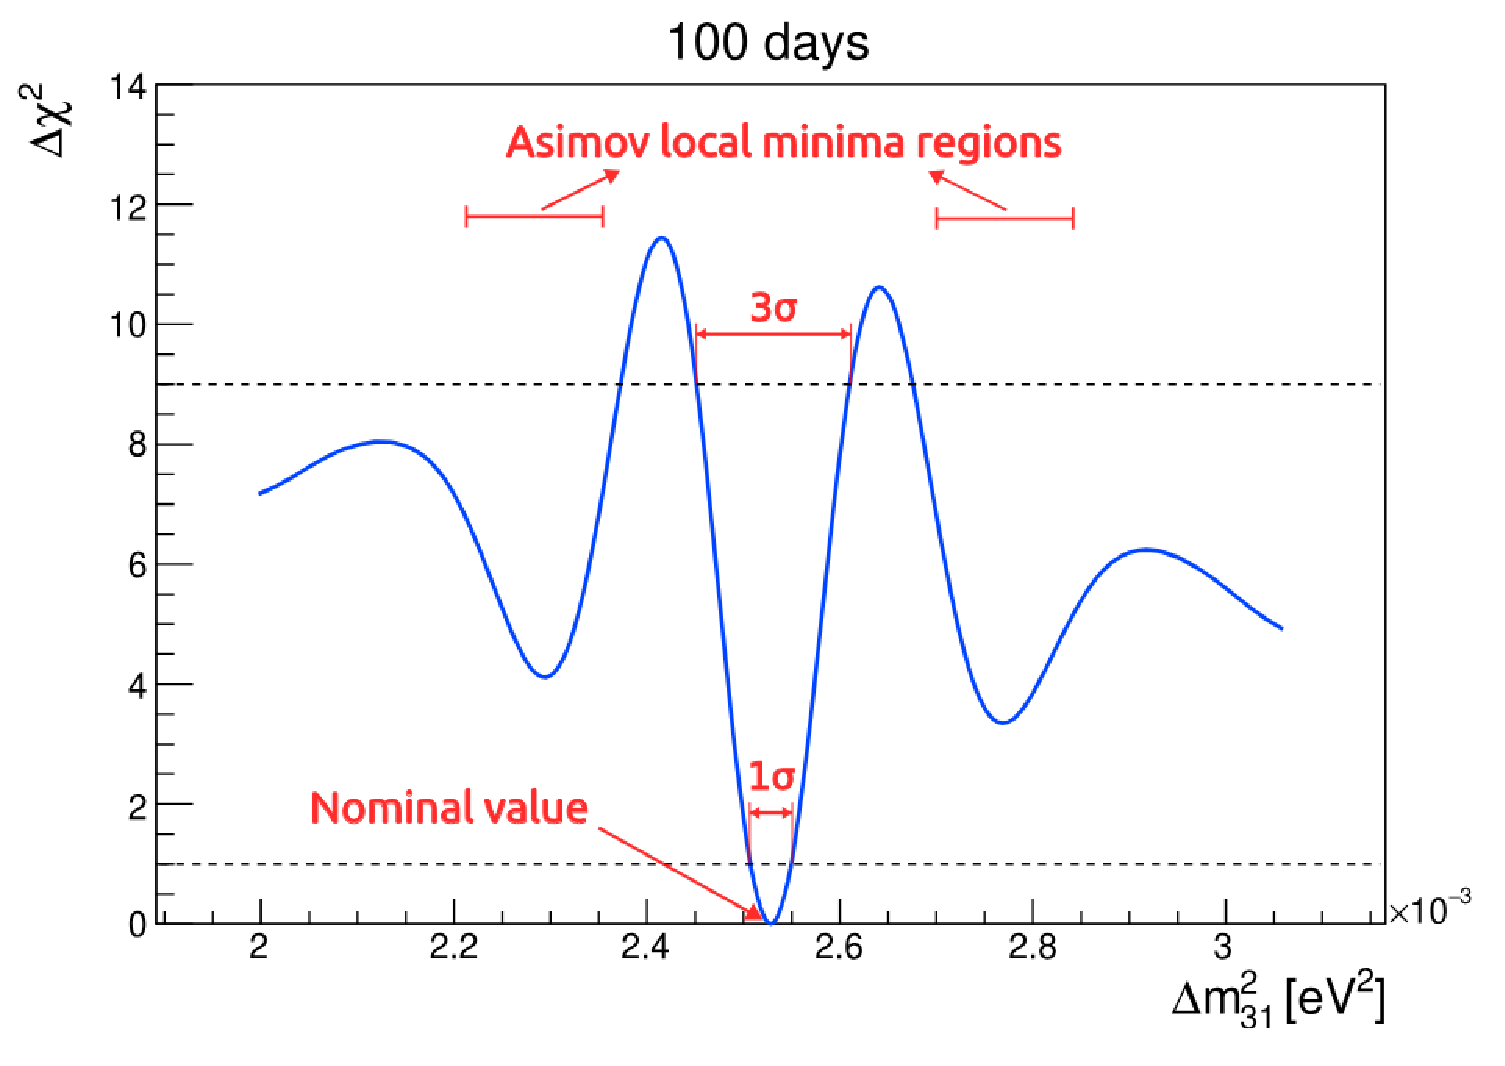
\includegraphics[width=1.\textwidth]{figs/Section2/benoitsteven_ProfileAsimov100d.pdf}
  \caption{\small $\chi^2$ profile: $\Delta \chi^2 = \chi^2 - \chi^2_{global}$ as a function of $\Delta m^2_{31}$, obtained by fitting to a 100-day Asimov dataset.}
  \label{fig:ProfileAsimov100d}
\end{figure}


\begin{figure}[!h]
  \centering
  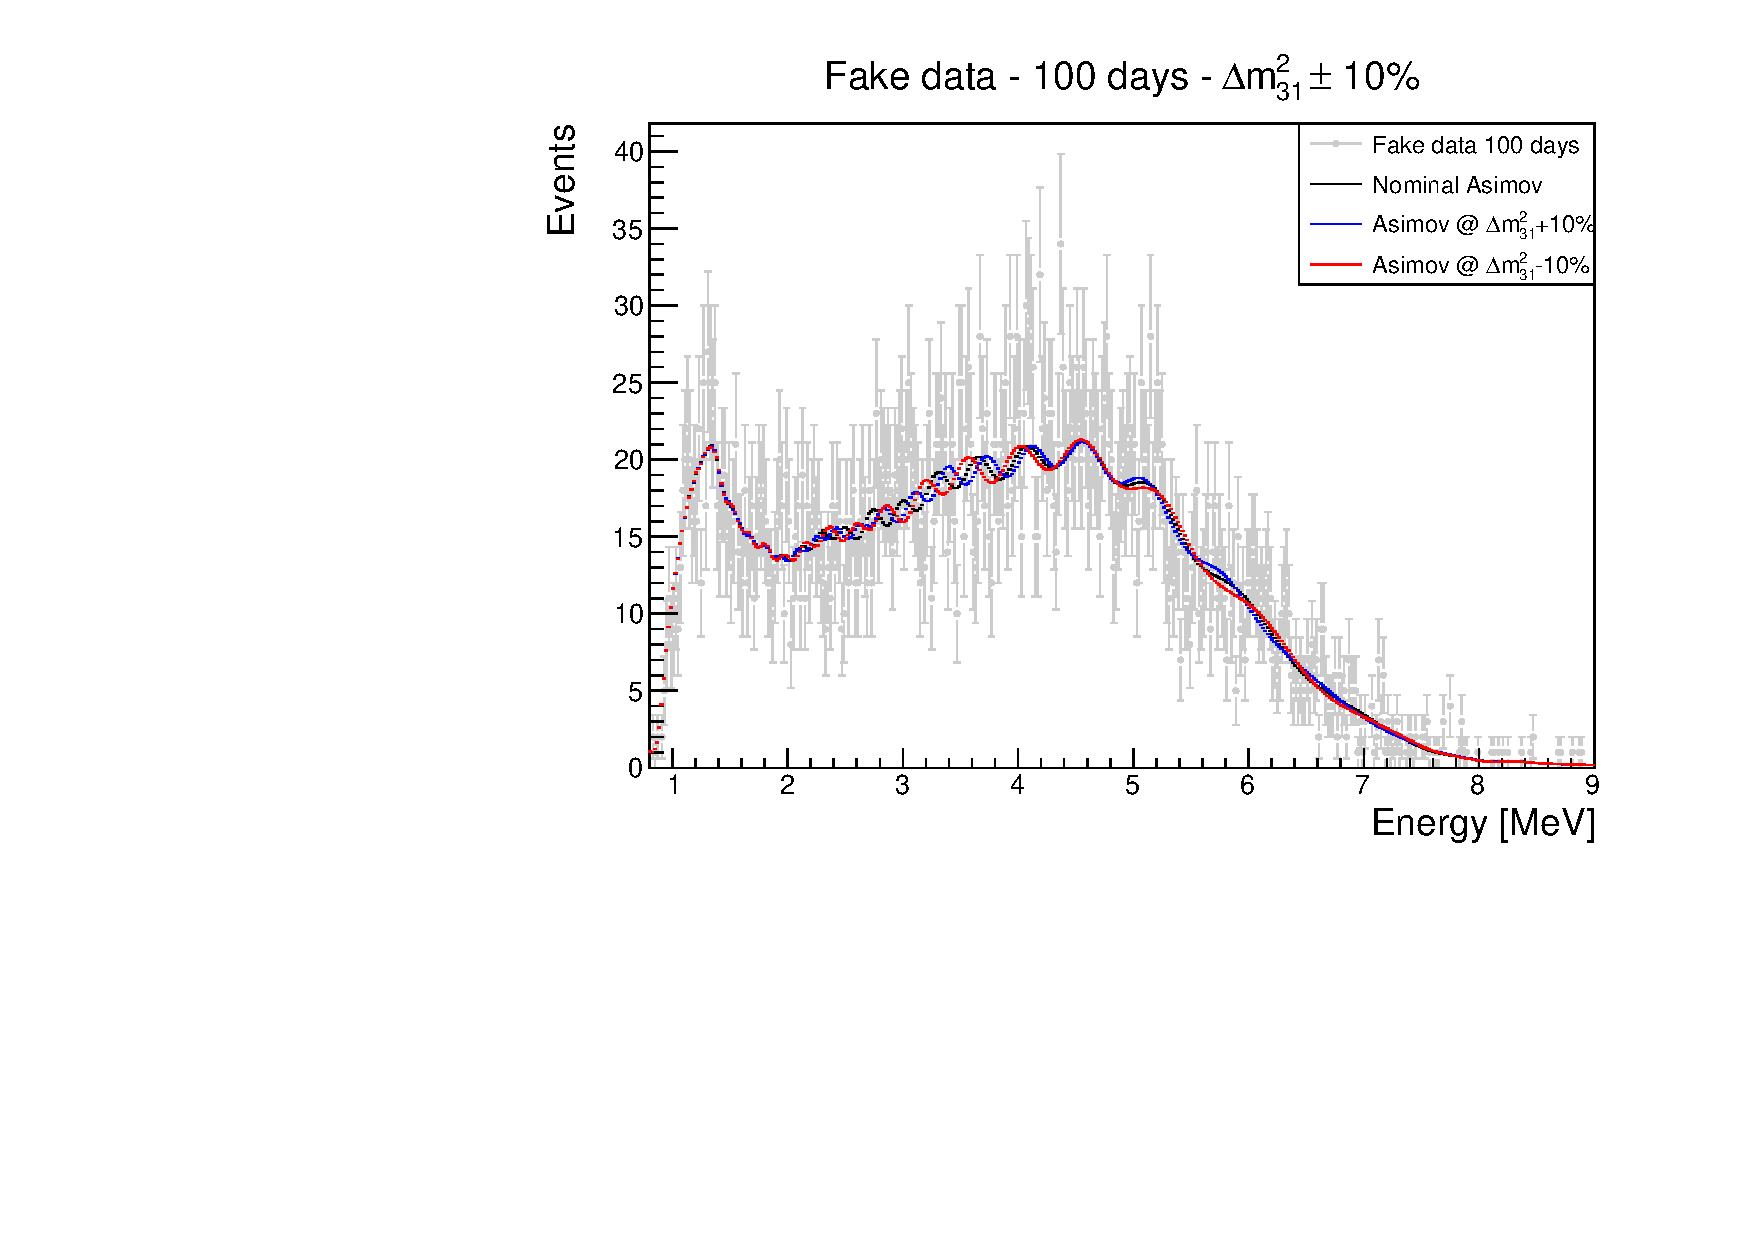
\includegraphics[width=1.\textwidth]{figs/Section2/benoitsteven_toy_100days_pm10percent.pdf}
  \caption{\small Theoretical visible Energy distribution for 3 assumed values of $\Delta m^2_{31}$,  superimposed with a pseudo-sample corresponding to 100 days of data taking. The assumed values differ by 10$\%$. This is similar to the difference observed in Fig.~\ref{fig:mosaic} between the true value of $\Delta m^2_{31}$ and the closest other minima. This illustrates that with low exposure, the data do not provide a strong enough constraint against these types of shifts in  $\Delta m^2_{31}$. }
  \label{fig:toy_E_spectrum_100days}
\end{figure}


%%%%%


%\begin{itemize}
%    \item Remind recently published sensitivities are based on this.
%    \item Remind the conditions under which Asimov sensitivities are valid.
%    \item Remind results
%    \begin{itemize}
%        \item $\longrightarrow$ Table: uncertainty on $\Delta m^2_{31}$ at various exposures.
%        \item $\longrightarrow$ Fig.: Parabolic profiles.
%    \end{itemize}
%    \item We had reasons to expect a more difficult measurement in the case of real data (with fluctuations), this called for a more realistic approach. 
%    \begin{itemize}
%        \item $\longrightarrow$ Fig: IO and NO theoretical spectra superimposed with a distribution with realistic fluctuations (expect several oscillation patterns to be consistent with data). 
%    \end{itemize}
%\end{itemize}

\subsection{JUNO's sensitivity to $\Delta m^2_{31}$ based on toy studies}\label{sec:senswithtoy}

The Task Force used four fit frameworks: ORSA, GNA, AveNuE and IHEP. A brief description of the methods they adopt can be found in Appendix~\ref{app:fit}.
These frameworks have been employed to generate pseudosamples and to perform oscillation fits on them, resulting in a collection of
$\chi^2$ profiles as a function of $\Delta m^2_{31}$. Fig.~\ref{fig:mosaic} presents, for each framework and three different exposures (100 days, 1 year, and 6 years), a set of 12 representative profiles. The study of the full collection confirms that, at low exposure levels, Asimov studies underestimate the impact of the issues introduced in Section~\ref{AsimLimit}.

Two key observations are quantified in Table~\ref{tab:BadMinKeyStatistics}. All frameworks consistently find that, with a 100-day dataset,  there is a more than a 30 $\%$ chance that the $\chi^2$ profile produces a disjoint CI. The sub-intervals are typically separated by a distance far greater than the Asimov resolution provided in Table~\ref{tab:AsimovSenstivity}. Also, there's a similar probability to obtain a single, contiguous CI, but located around a bad minimum. Such scenarios would induce a tension with world averages. 
These issues are much worse at lower exposures and mitigated with higher statistics. However, they are still significant for
measurements based on 1 year of data taking. We also notice that even at low exposures, profiles resulting in a single, contiguous CI, located around the true value of $\Delta m^2_{31}$,  are still common and that the corresponding 1$\sigma$ uncertainty is often lower than the Asimov prediction. Therefore, even at low exposure, it is not unlikely to produce a result that could be used within  the neutrino community to produce a highly significant constraint on the NMO. 

These findings raise a series of questions. Should JUNO publish a measurement of $\Delta m^2_{31}$ based on JUNO's early data alone? Can a single confidence interval be obtained by incorporating an external constraint based on prior measurements of $\Delta m^2_{31}$ by reactor or accelerator experiments? The	observations made here also motivate verifying that the conditions necessary for Wilks' theorem to apply 
are satisfied. If not, what statistical procedure should be applied to ensure a correct coverage for the confidence interval? These questions are addressed in the remainder of this report. 
    
\begin{figure}[h!]
\centering
\begin{tabular}{cccc}
% Row 1
\begin{subfigure}[b]{0.24\textwidth}
    \centering
    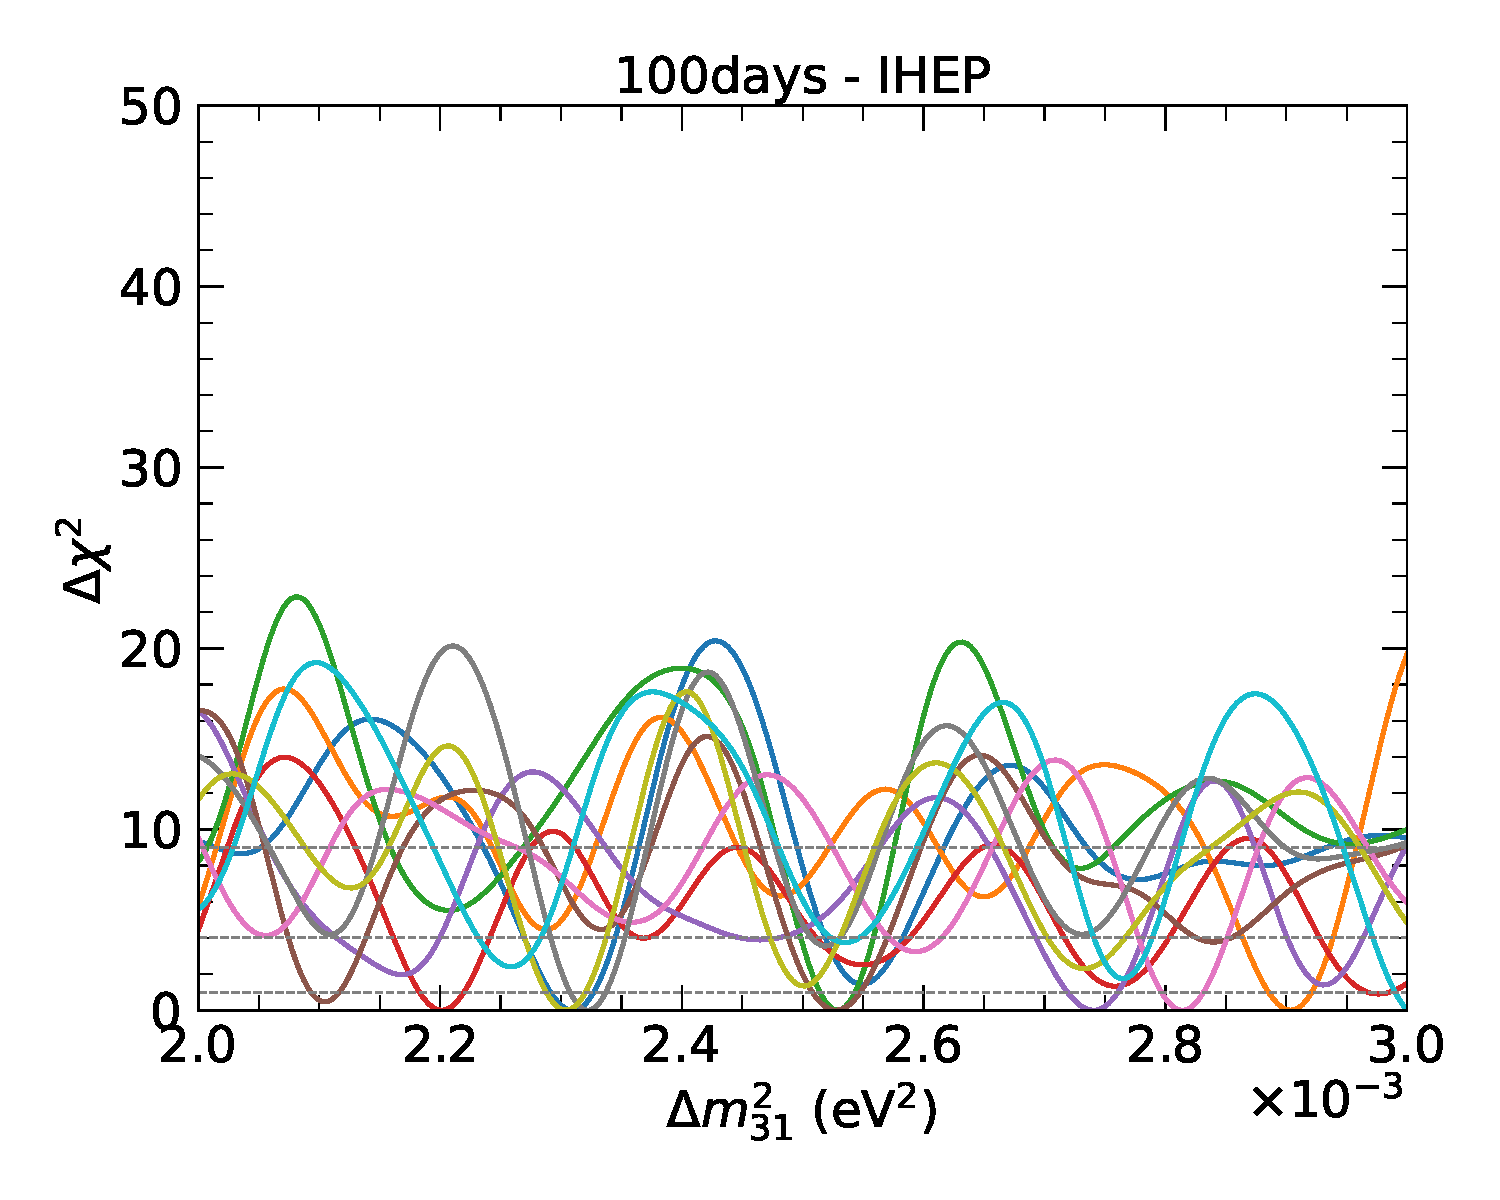
\includegraphics[width=\textwidth]{figs/Section2/Jingqin_100days_dmsq31_profile.pdf}
    \caption{ }
\end{subfigure} &
\begin{subfigure}[b]{0.24\textwidth}
    \centering
    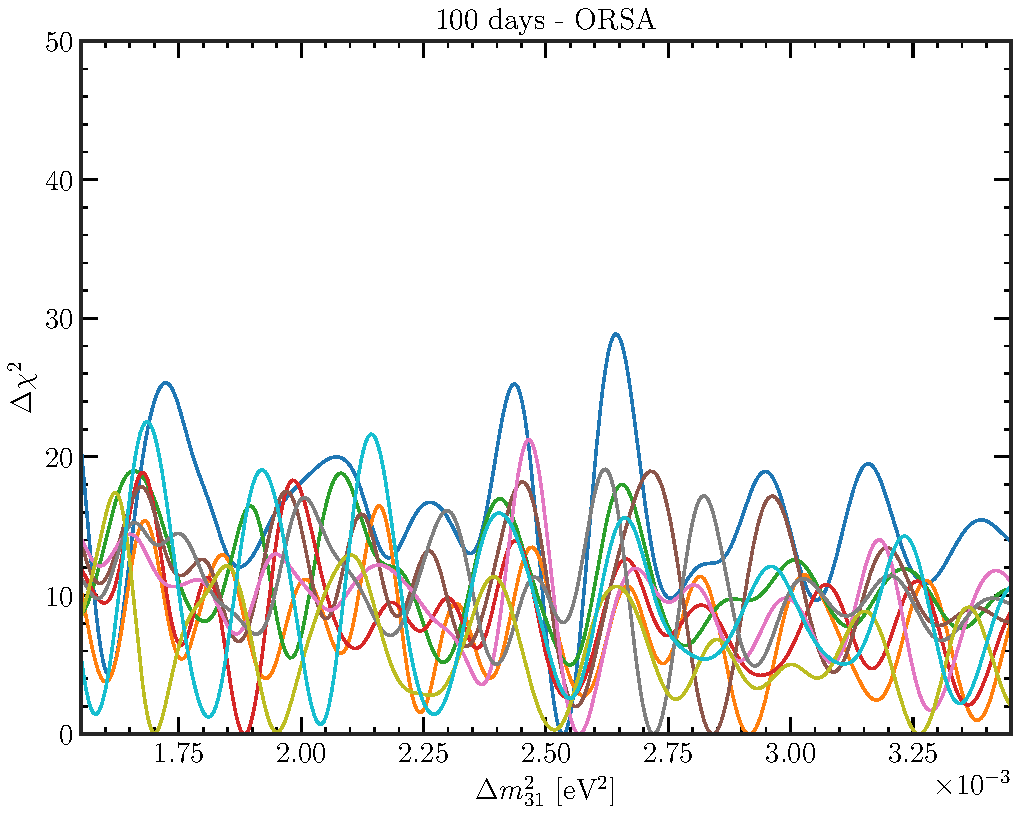
\includegraphics[width=0.94\textwidth]{figs/Section2/vanessa_profiles_100d.pdf}
    \caption{ }
\end{subfigure} &
\begin{subfigure}[b]{0.24\textwidth}
    \centering
    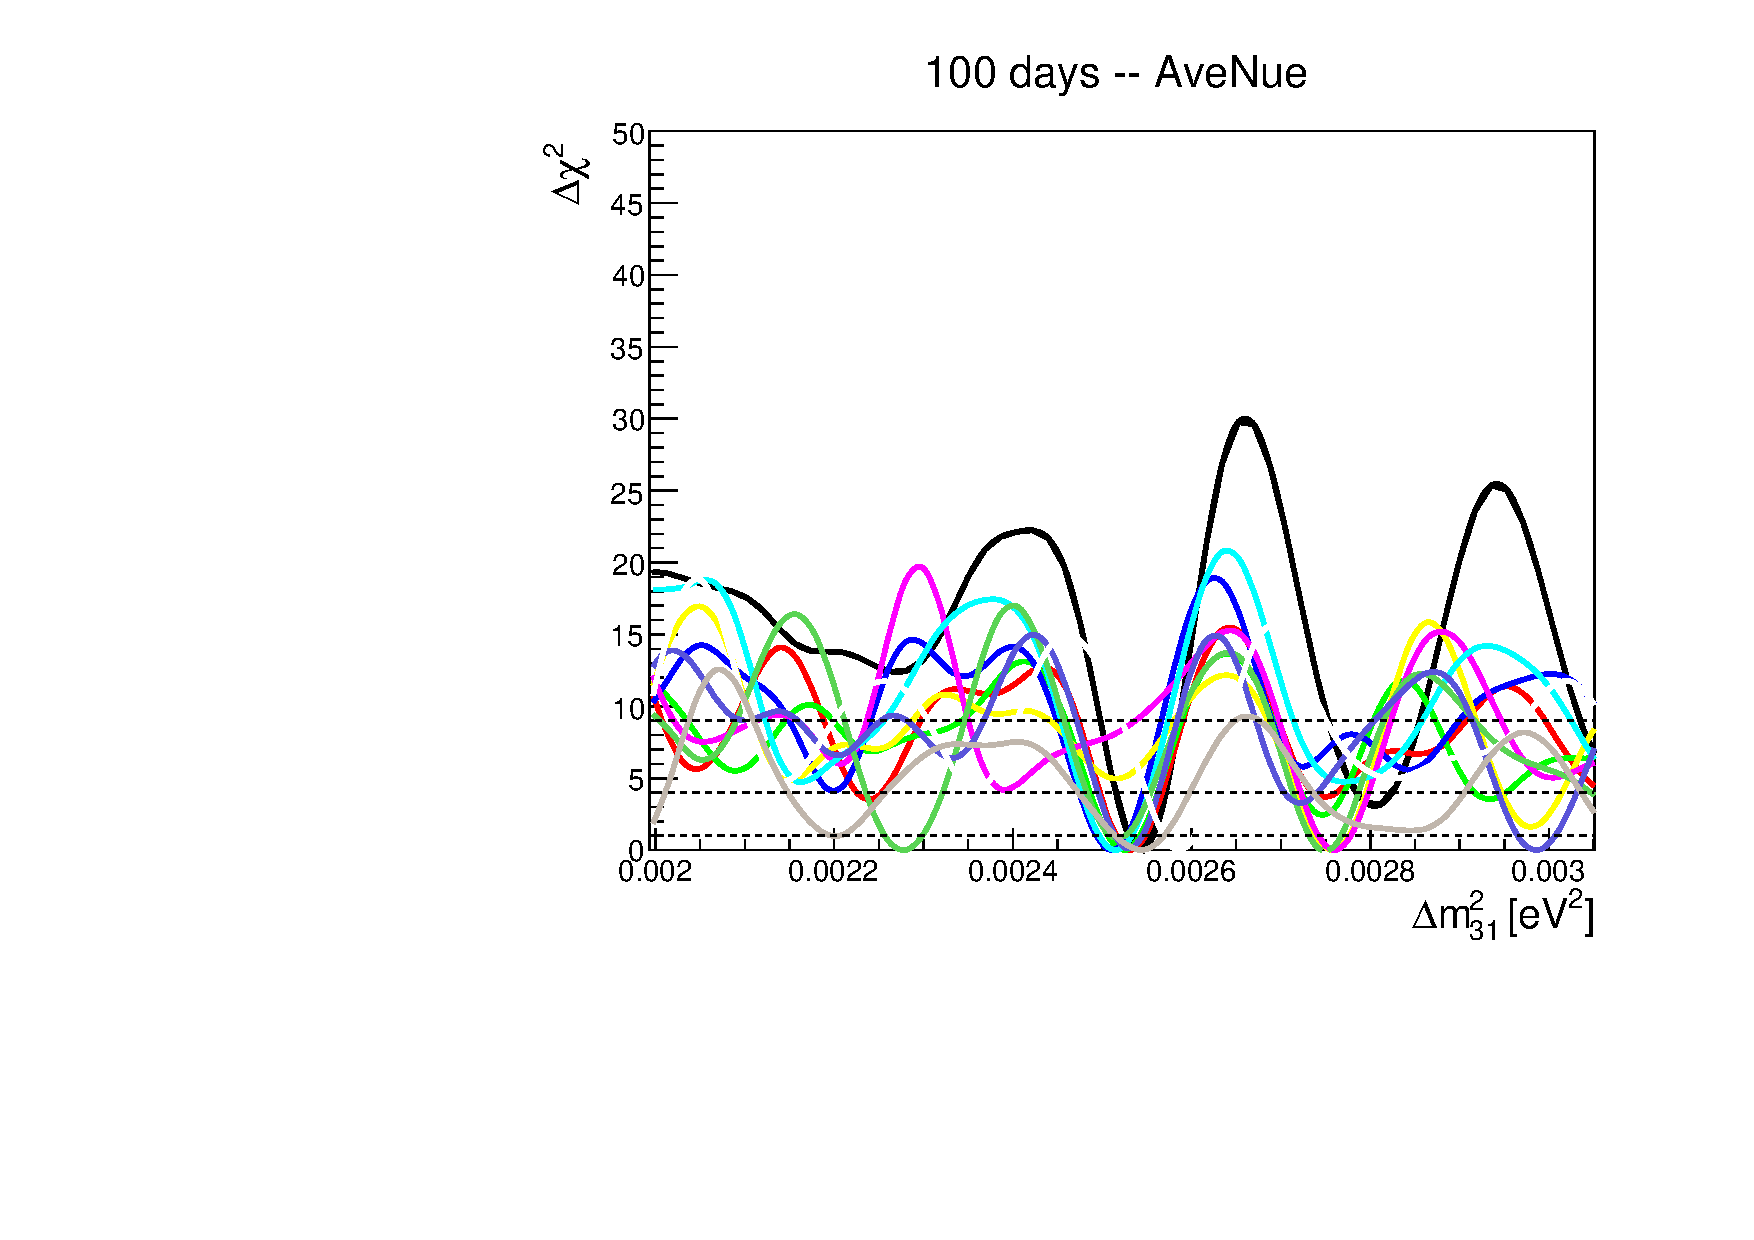
\includegraphics[width=\textwidth]{figs/Section2/benoitsteven_Prof_100d.pdf}
    \caption{ }
\end{subfigure}
\begin{subfigure}[b]{0.24\textwidth}
    \centering
    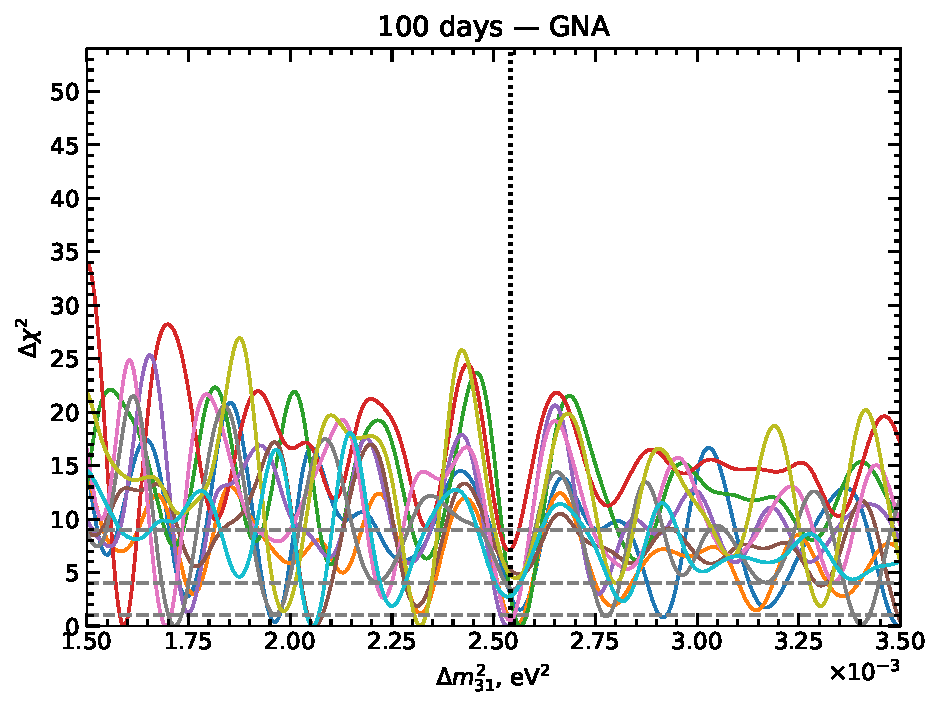
\includegraphics[width=\textwidth]{figs/Section2/dmitry_profiles_100d.pdf}
    \caption{ }
\end{subfigure} \\
% Row 2
\begin{subfigure}[b]{0.24\textwidth}
    \centering
    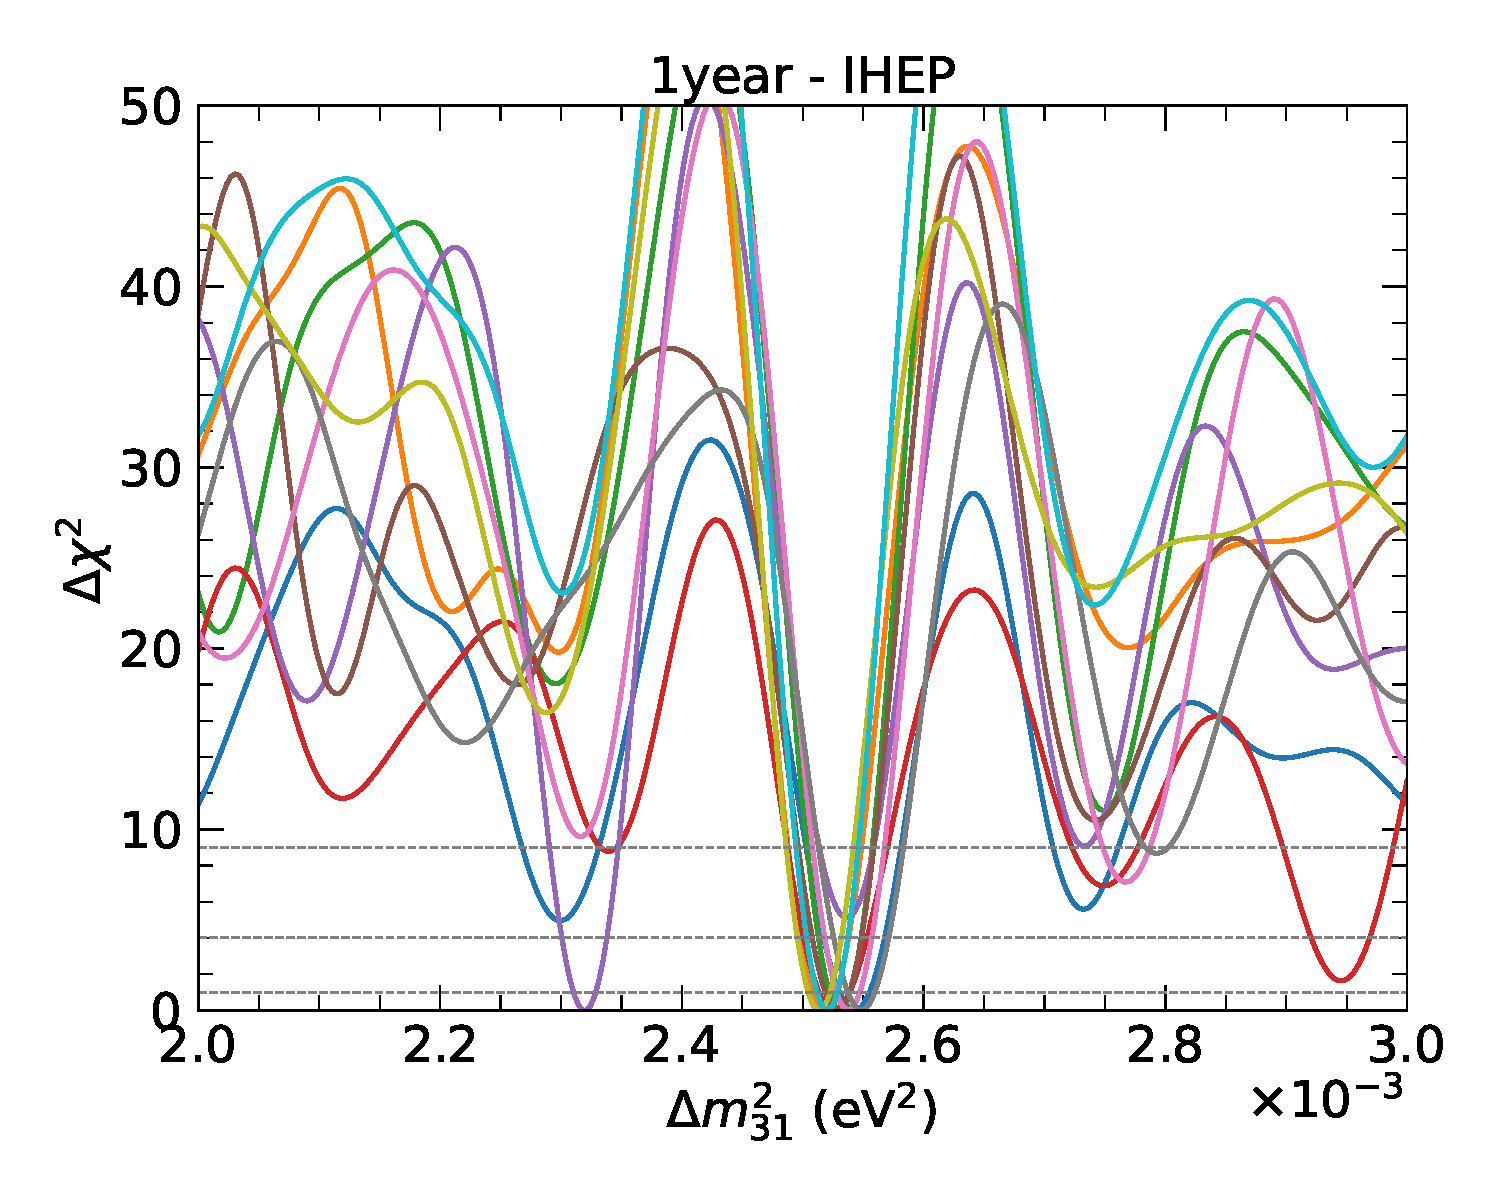
\includegraphics[width=\textwidth]{figs/Section2/Jingqin_1years_dmsq31_profile.pdf}
    \caption{ }
\end{subfigure} &
\begin{subfigure}[b]{0.24\textwidth}
    \centering
    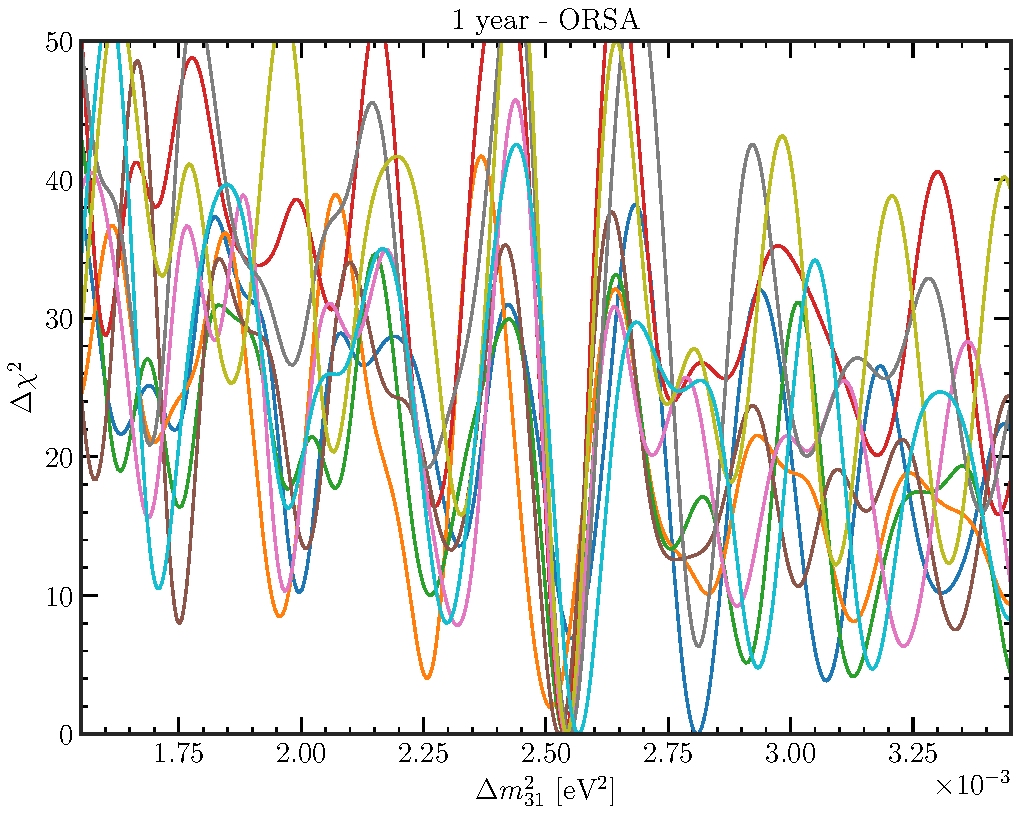
\includegraphics[width=0.94\textwidth]{figs/Section2/vanessa_profiles_1y.pdf}
    \caption{ }
\end{subfigure} &
\begin{subfigure}[b]{0.24\textwidth}
    \centering
    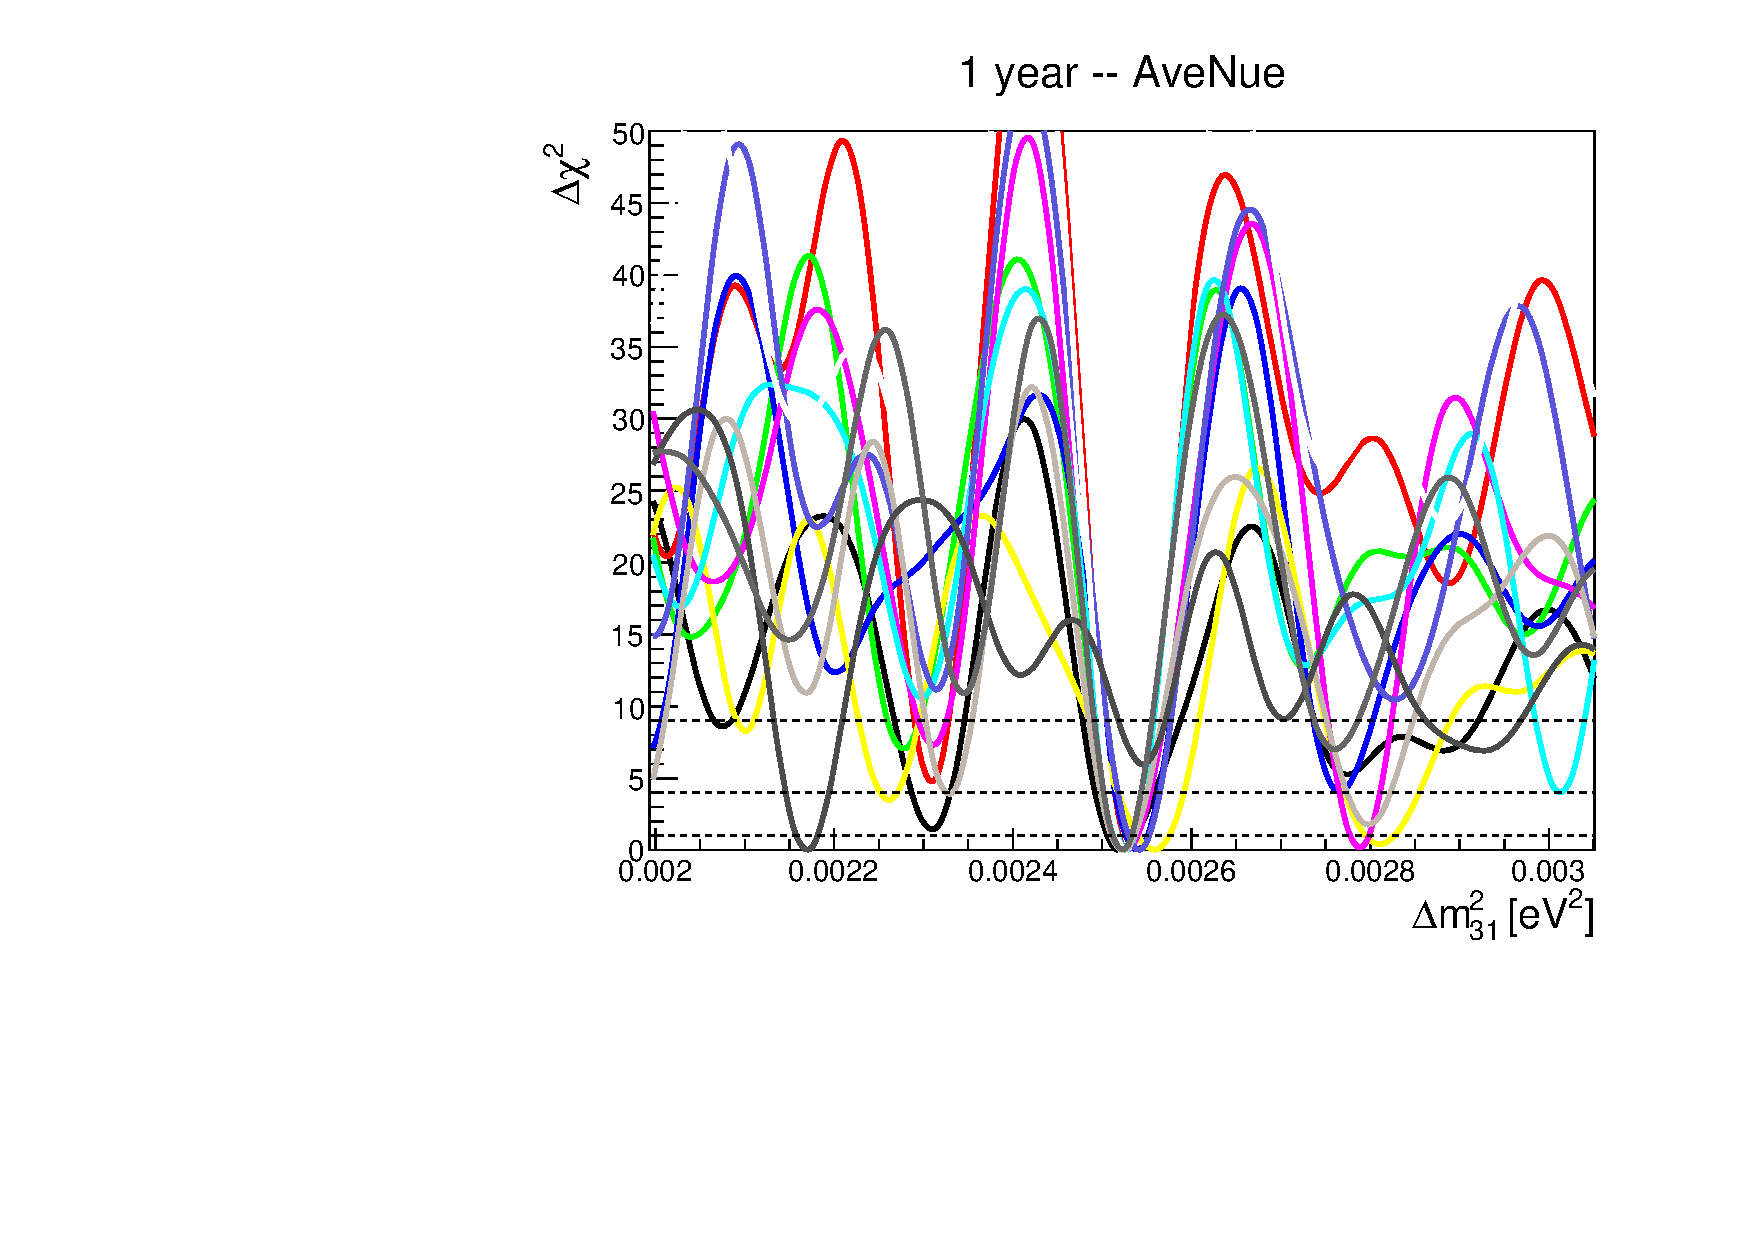
\includegraphics[width=\textwidth]{figs/Section2/benoitsteven_Prof_1yr.pdf}
    \caption{ }
\end{subfigure}
\begin{subfigure}[b]{0.24\textwidth}
    \centering
    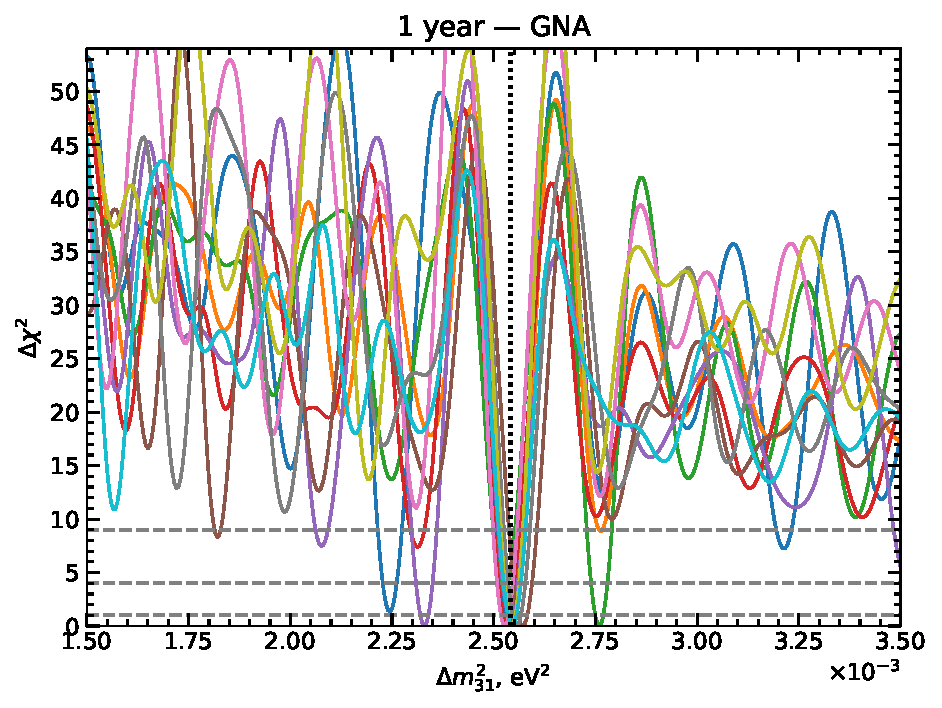
\includegraphics[width=\textwidth]{figs/Section2/dmitry_profiles_1y.pdf}
    \caption{ }
\end{subfigure} \\
% Row 3
\begin{subfigure}[b]{0.24\textwidth}
    \centering
    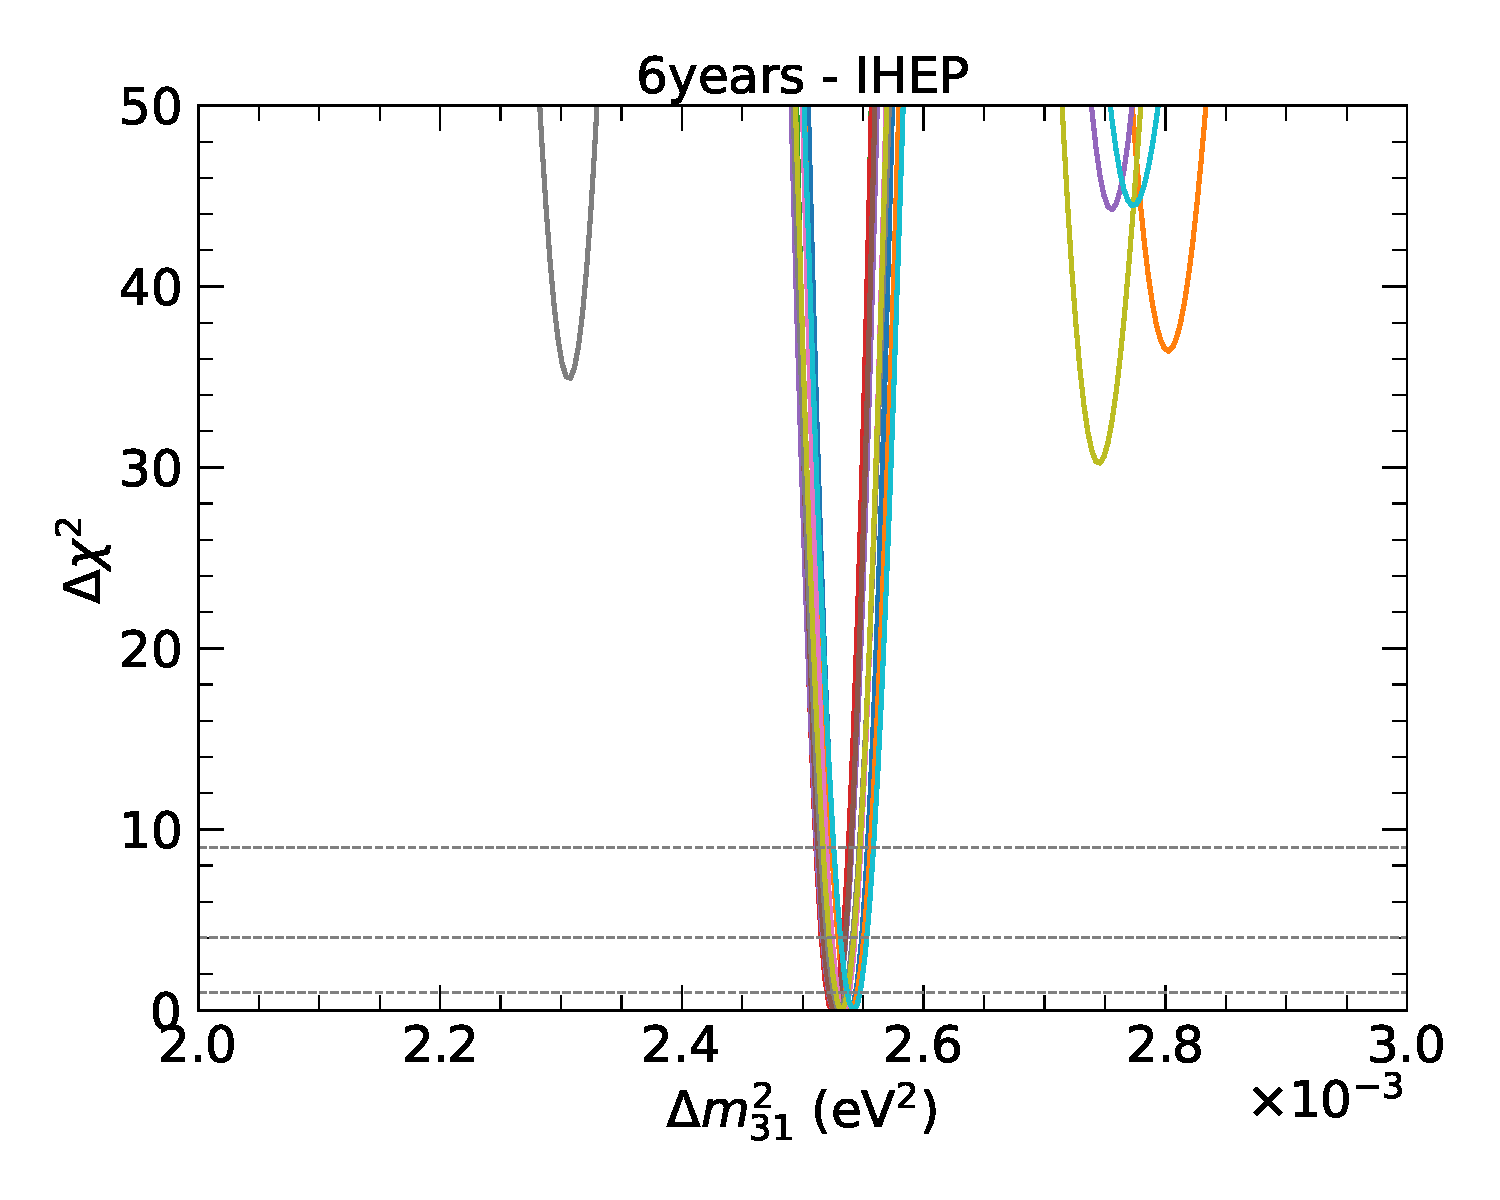
\includegraphics[width=\textwidth]{figs/Section2/Jingqin_6years_dmsq31_profile.pdf}
    \caption{ }
\end{subfigure} &
\begin{subfigure}[b]{0.24\textwidth}
    \centering
    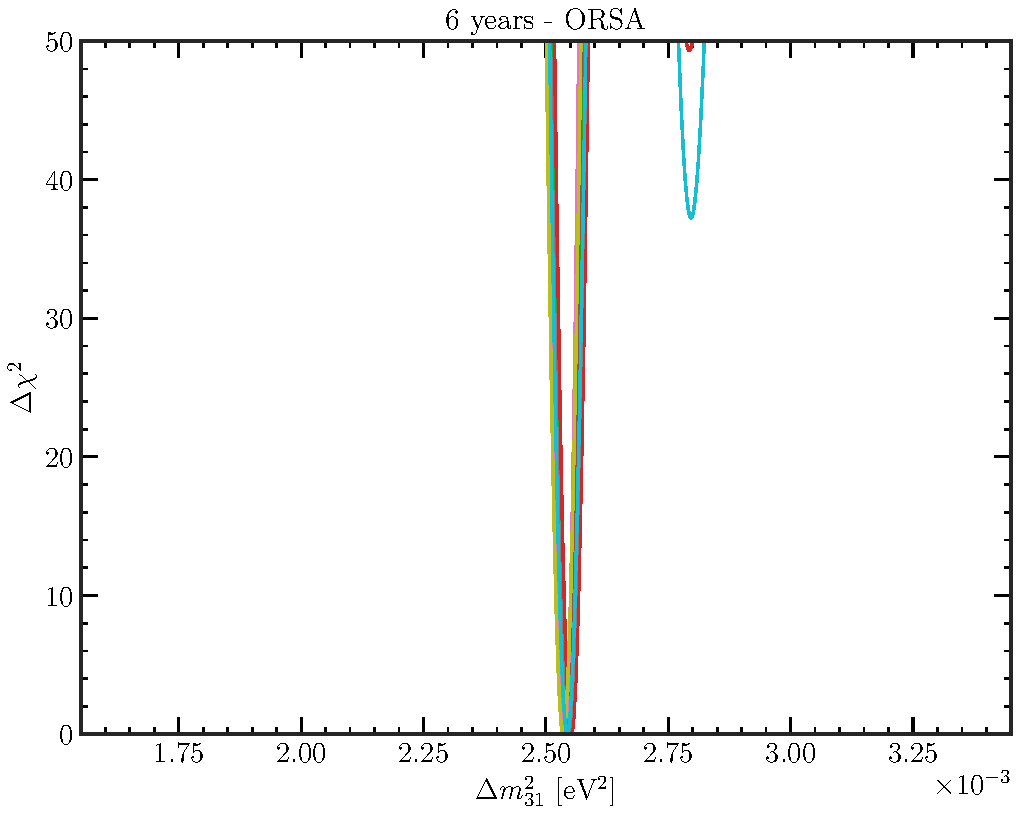
\includegraphics[width=0.94\textwidth]{figs/Section2/vanessa_profiles_6y.pdf}
    \caption{ }
\end{subfigure} &
\begin{subfigure}[b]{0.24\textwidth}
    \centering
    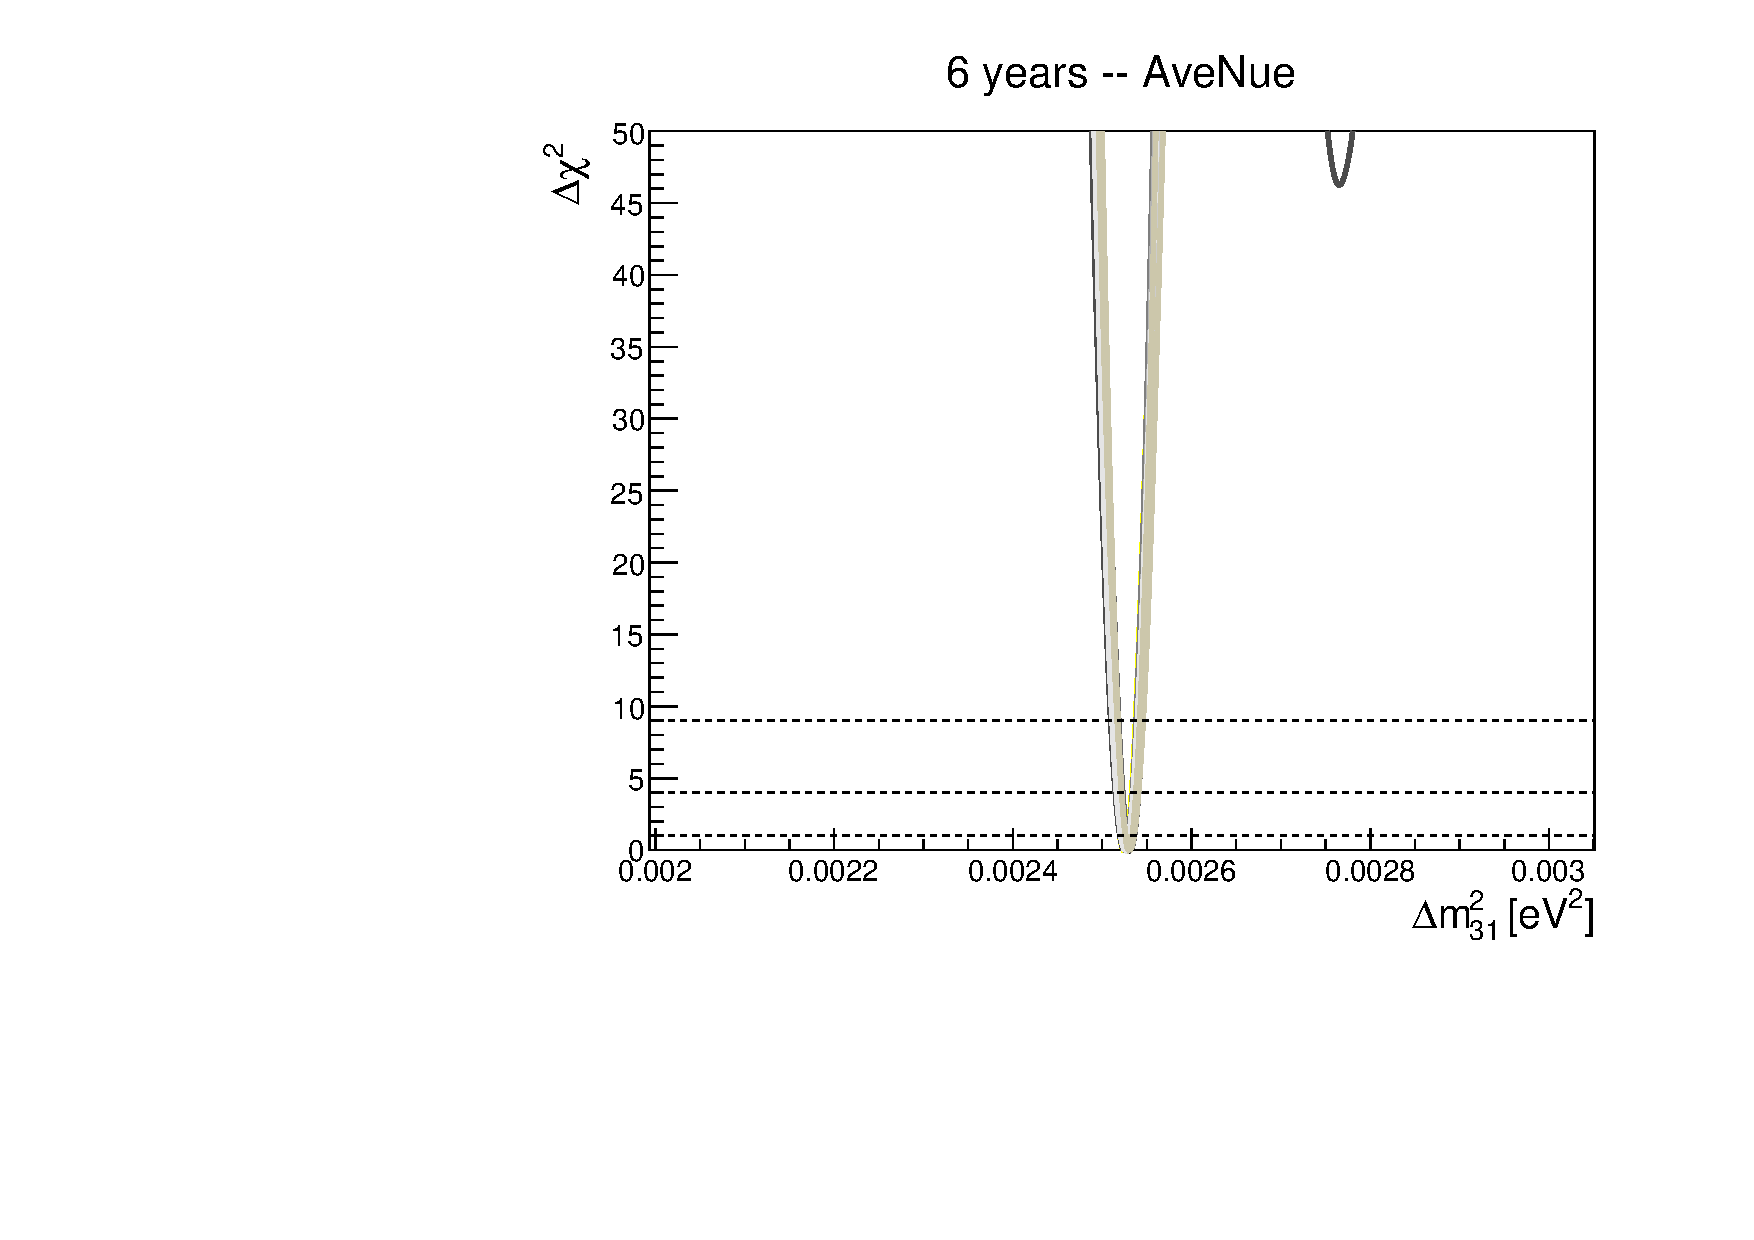
\includegraphics[width=\textwidth]{figs/Section2/benoitsteven_Prof_6yrs.pdf}
    \caption{ }
\end{subfigure}
\begin{subfigure}[b]{0.24\textwidth}
    \centering
    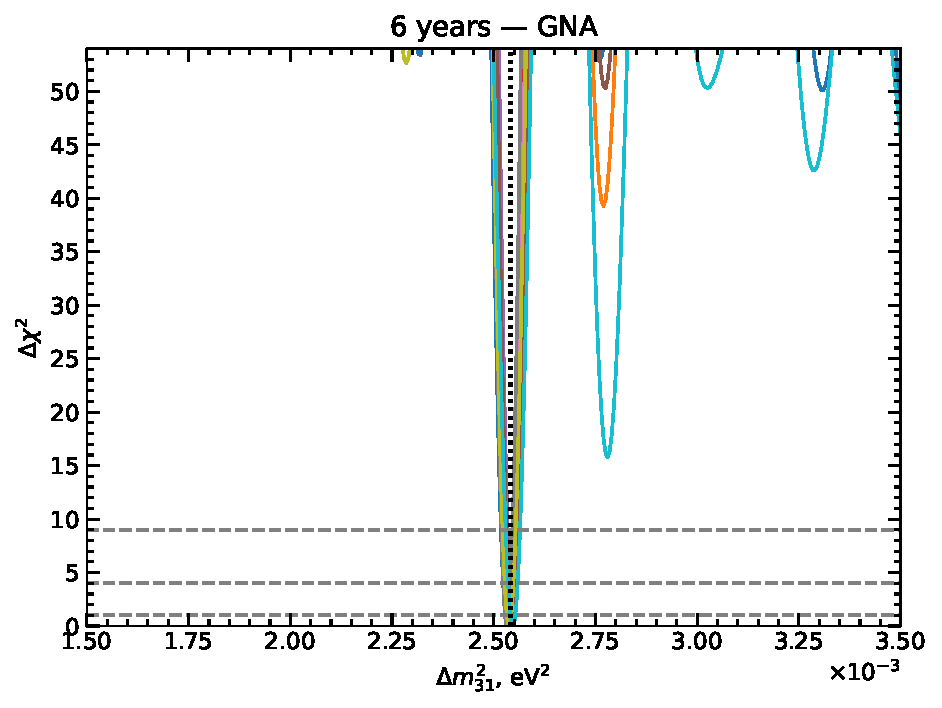
\includegraphics[width=\textwidth]{figs/Section2/dmitry_profiles_6y.pdf}
    \caption{ }
\end{subfigure} \\
\end{tabular}
\caption{$\chi^2$ profiles obtained by 4 frameworks, for 3 exposures}
\label{fig:mosaic}
\end{figure}


\begin{comment}
    
\begin{figure}[h!]
\centering
\begin{tabular}{cccc}
% Row 1
\begin{subfigure}[b]{0.24\textwidth}
    \centering
    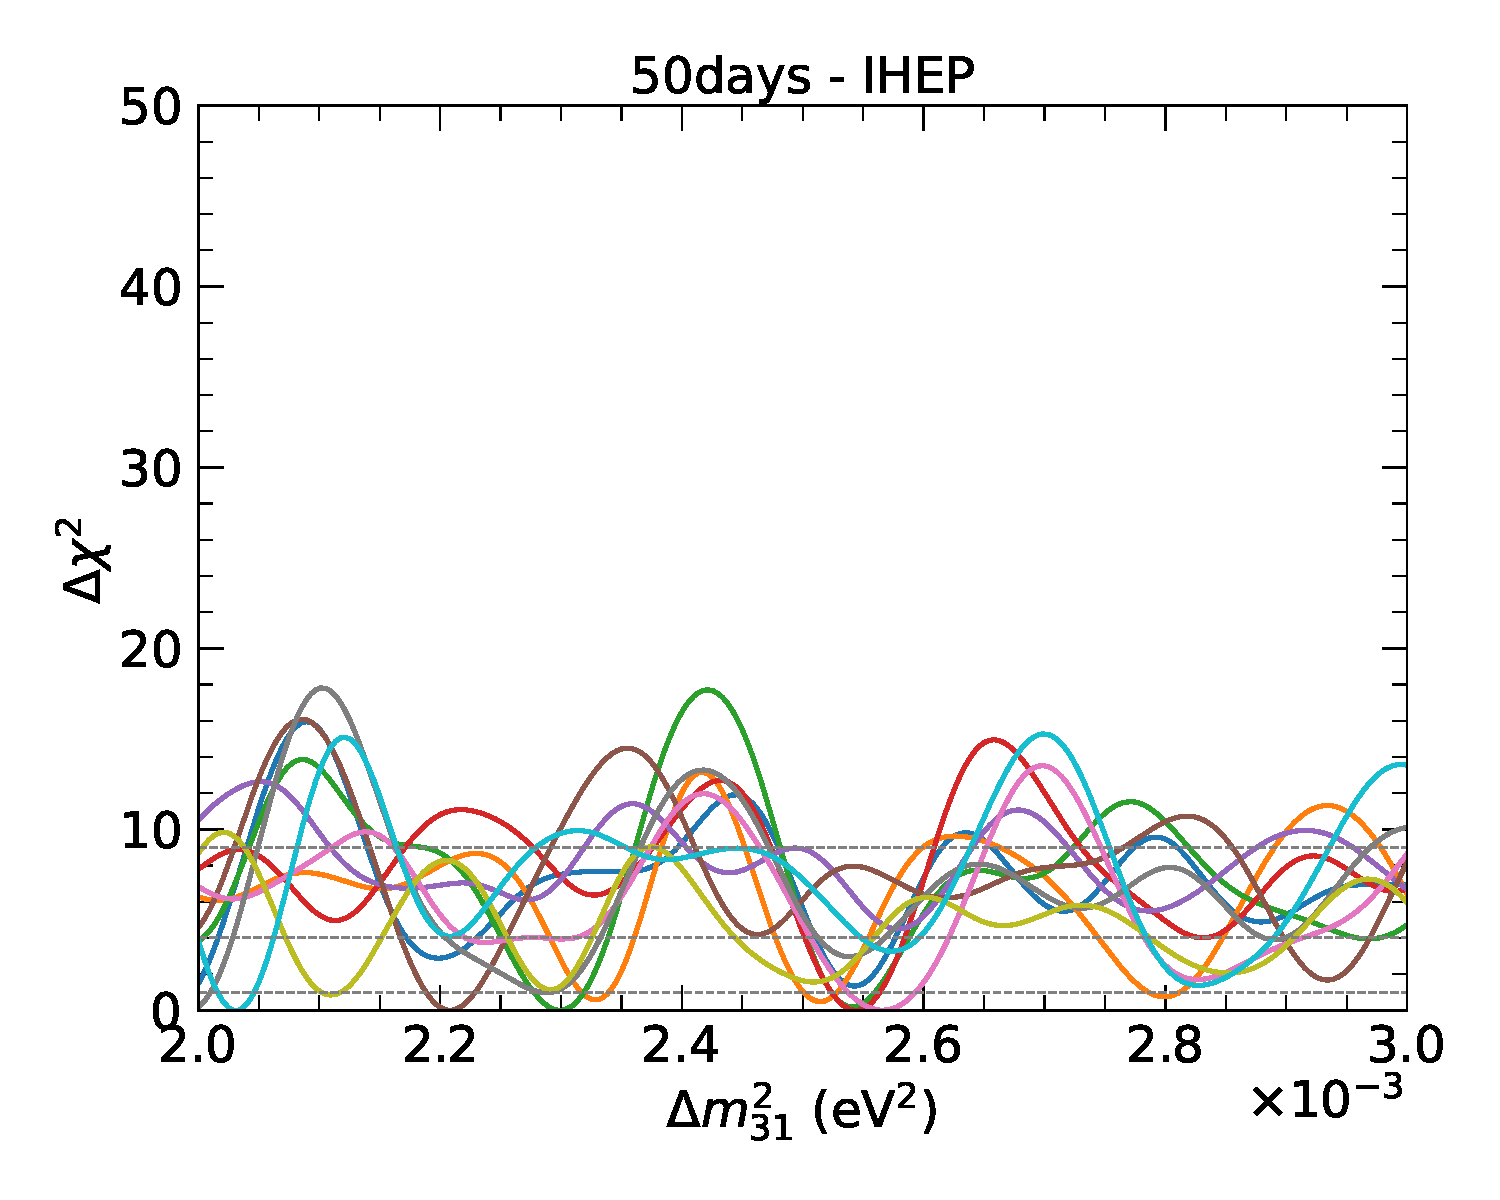
\includegraphics[width=\textwidth]{figs/Section2/Jingqin_50days_dmsq31_profile.pdf}
    \caption{ }
\end{subfigure} &
\begin{subfigure}[b]{0.24\textwidth}
    \centering
    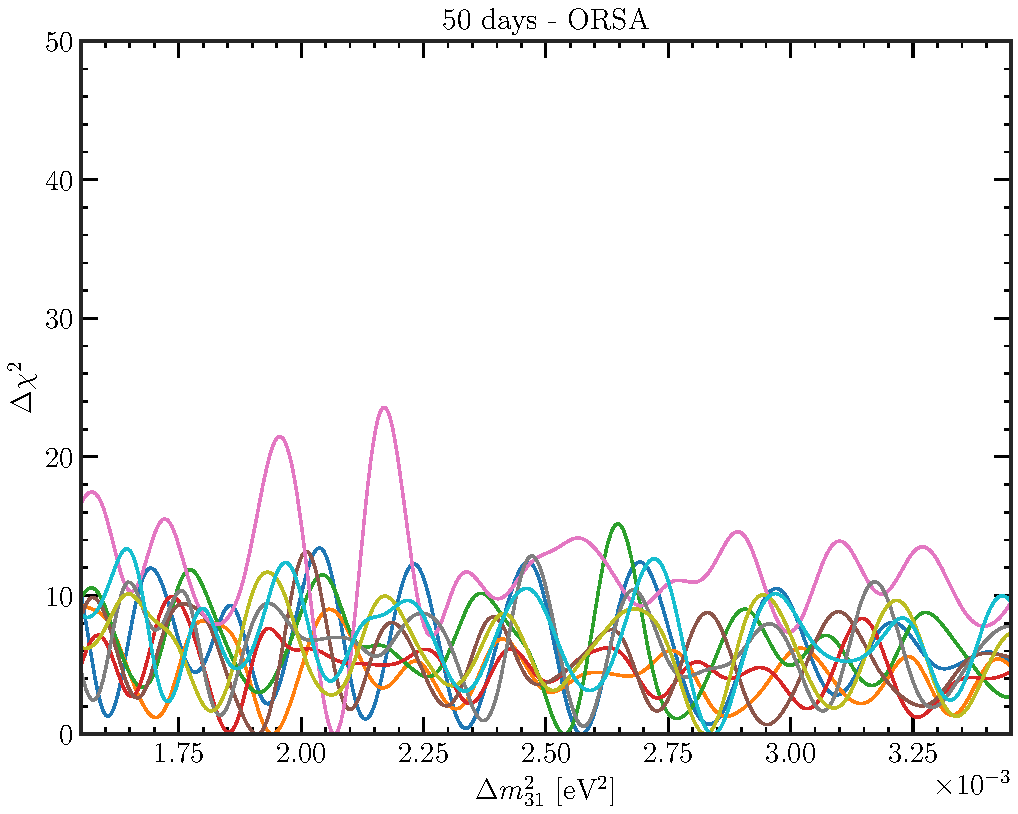
\includegraphics[width=0.94\textwidth]{figs/Section2/vanessa_profiles_50d.pdf}
    \caption{ } 
\end{subfigure} &
\begin{subfigure}[b]{0.24\textwidth}
    \centering
    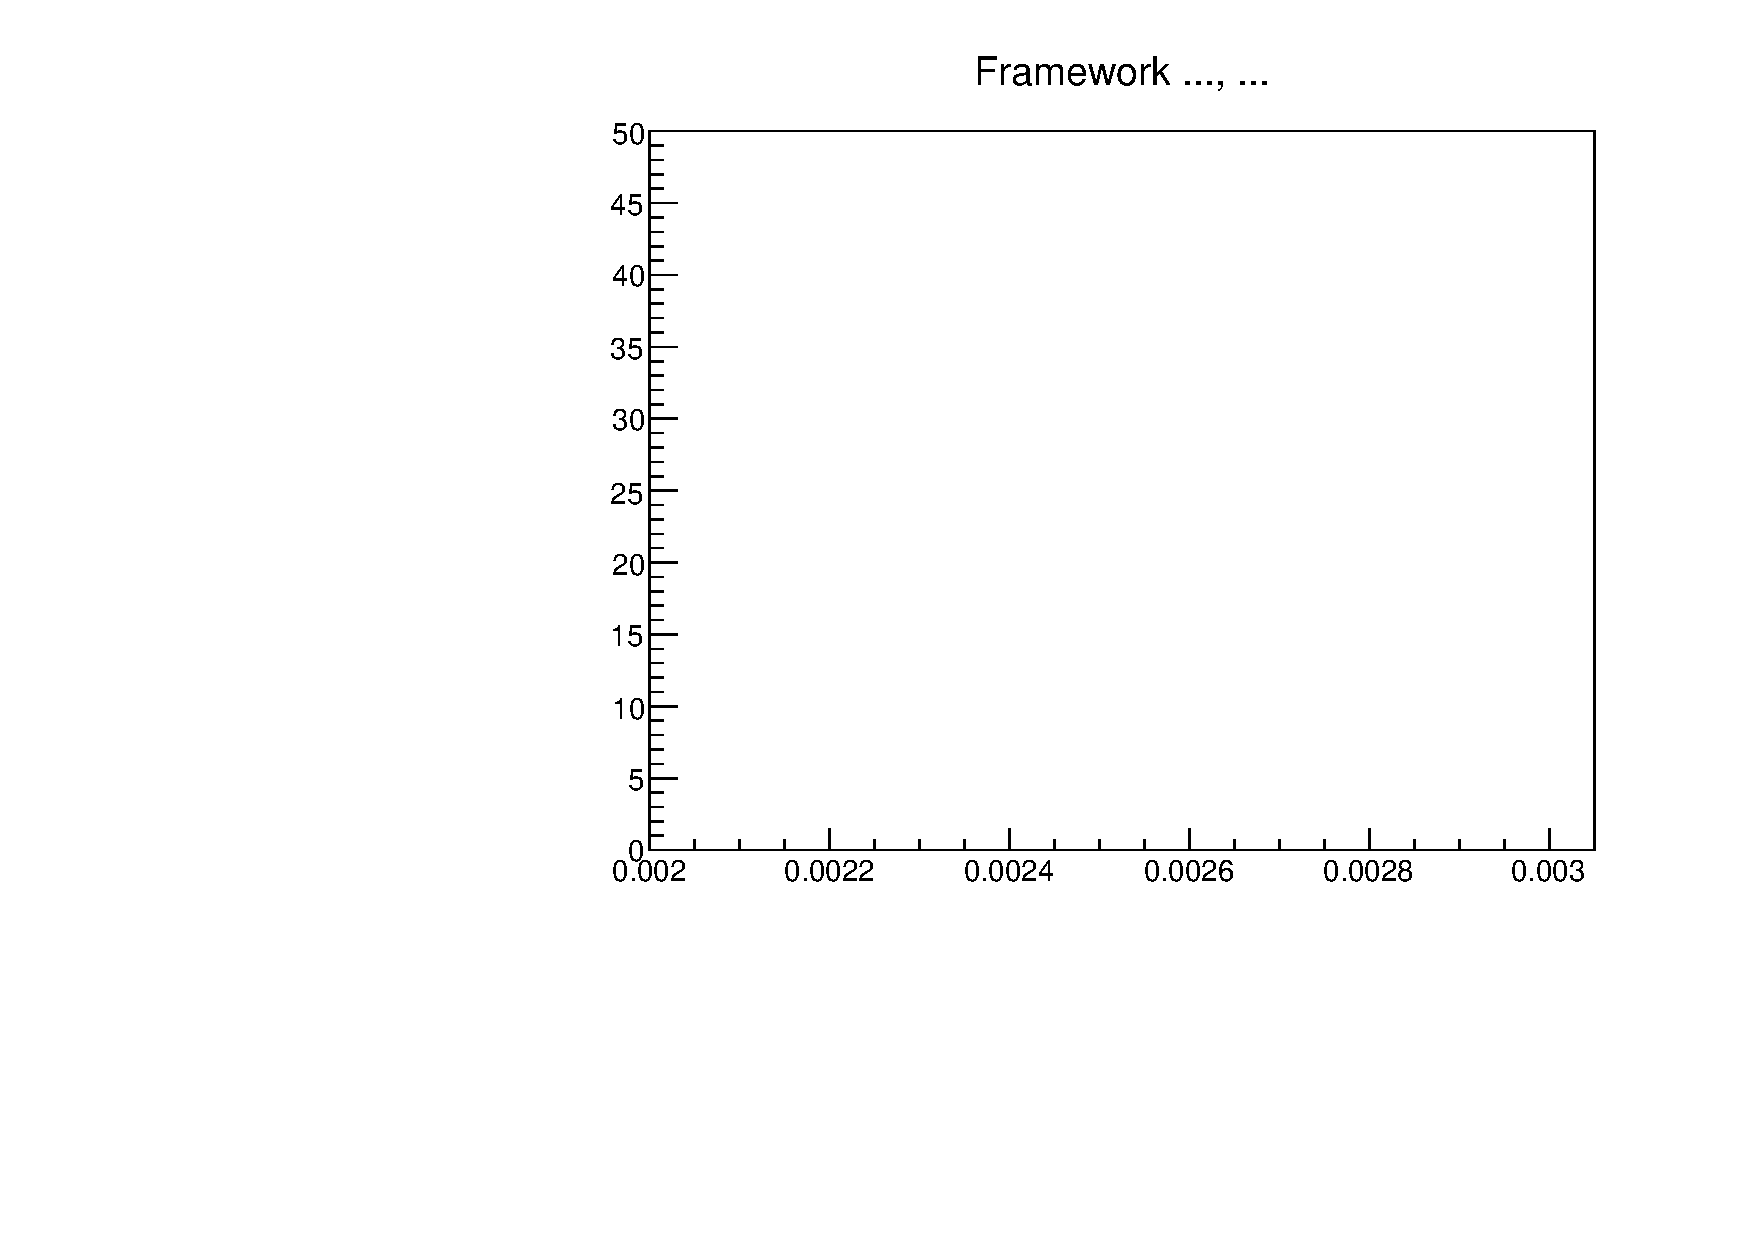
\includegraphics[width=\textwidth]{figs/Section2/benoitsteven_Prof_Generic.pdf}
    \caption{ }
\end{subfigure}
\begin{subfigure}[b]{0.24\textwidth}
    \centering
    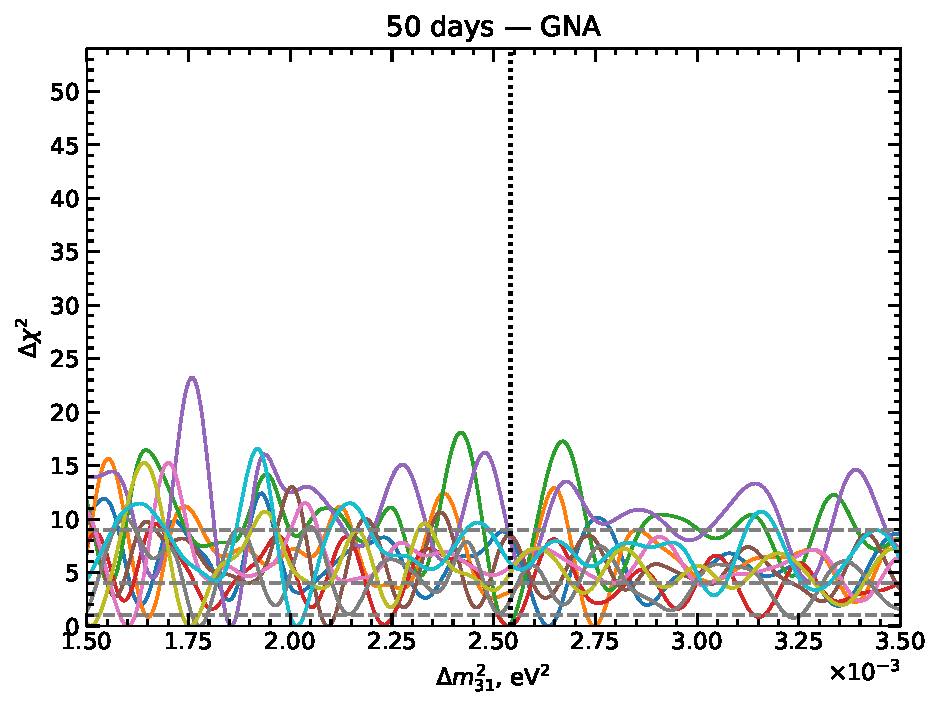
\includegraphics[width=\textwidth]{figs/Section2/dmitry_profiles_50d.pdf}
    \caption{ }
\end{subfigure} \\
% Row 2
\begin{subfigure}[b]{0.24\textwidth}
    \centering
    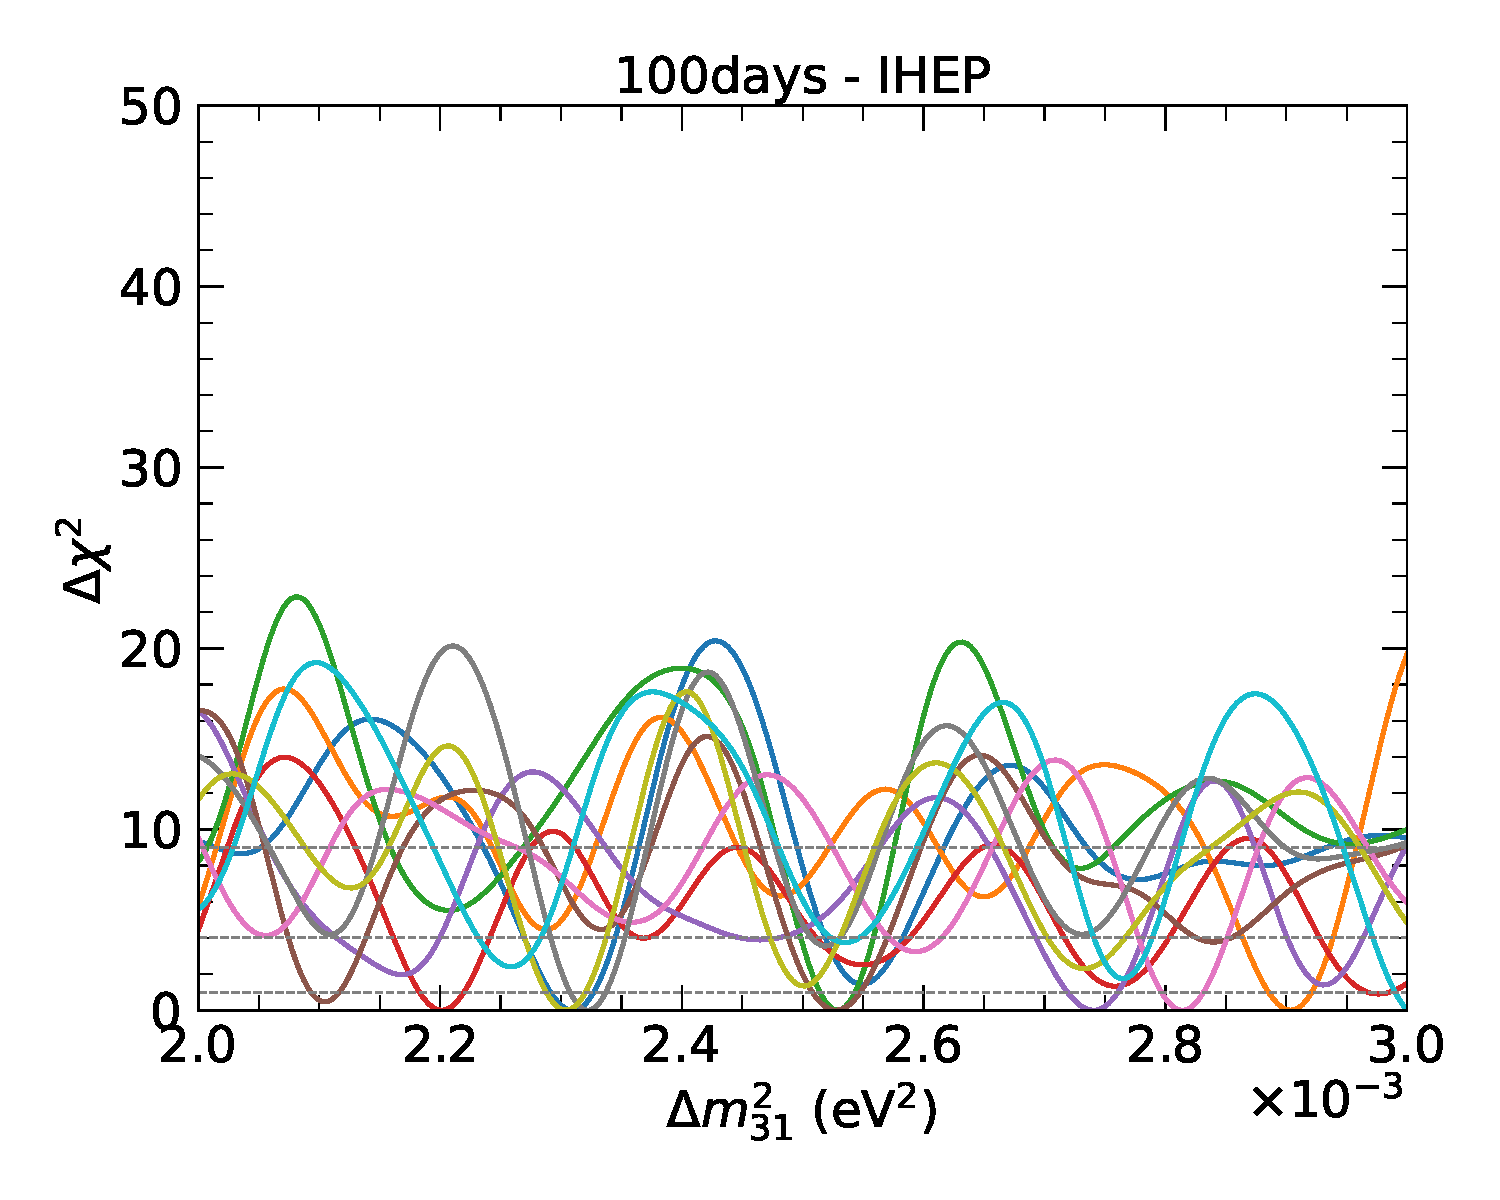
\includegraphics[width=\textwidth]{figs/Section2/Jingqin_100days_dmsq31_profile.pdf}
    \caption{ }
\end{subfigure} &
\begin{subfigure}[b]{0.24\textwidth}
    \centering
    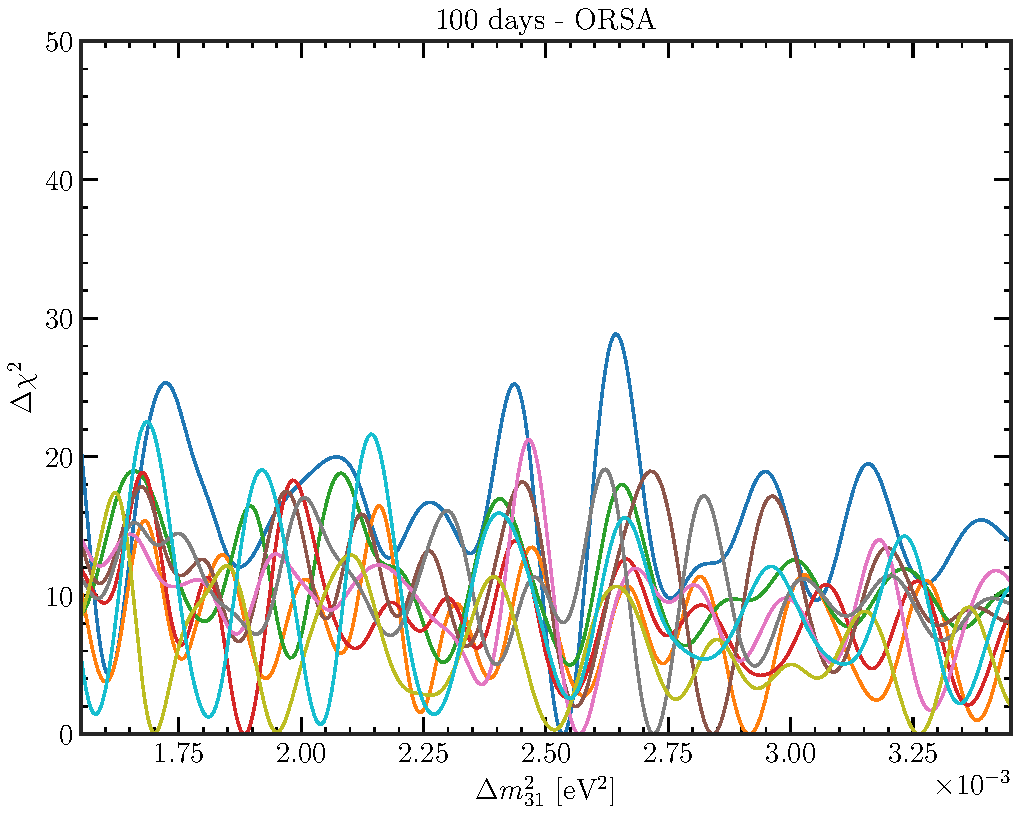
\includegraphics[width=0.94\textwidth]{figs/Section2/vanessa_profiles_100d.pdf}
    \caption{ }
\end{subfigure} &
\begin{subfigure}[b]{0.24\textwidth}
    \centering
    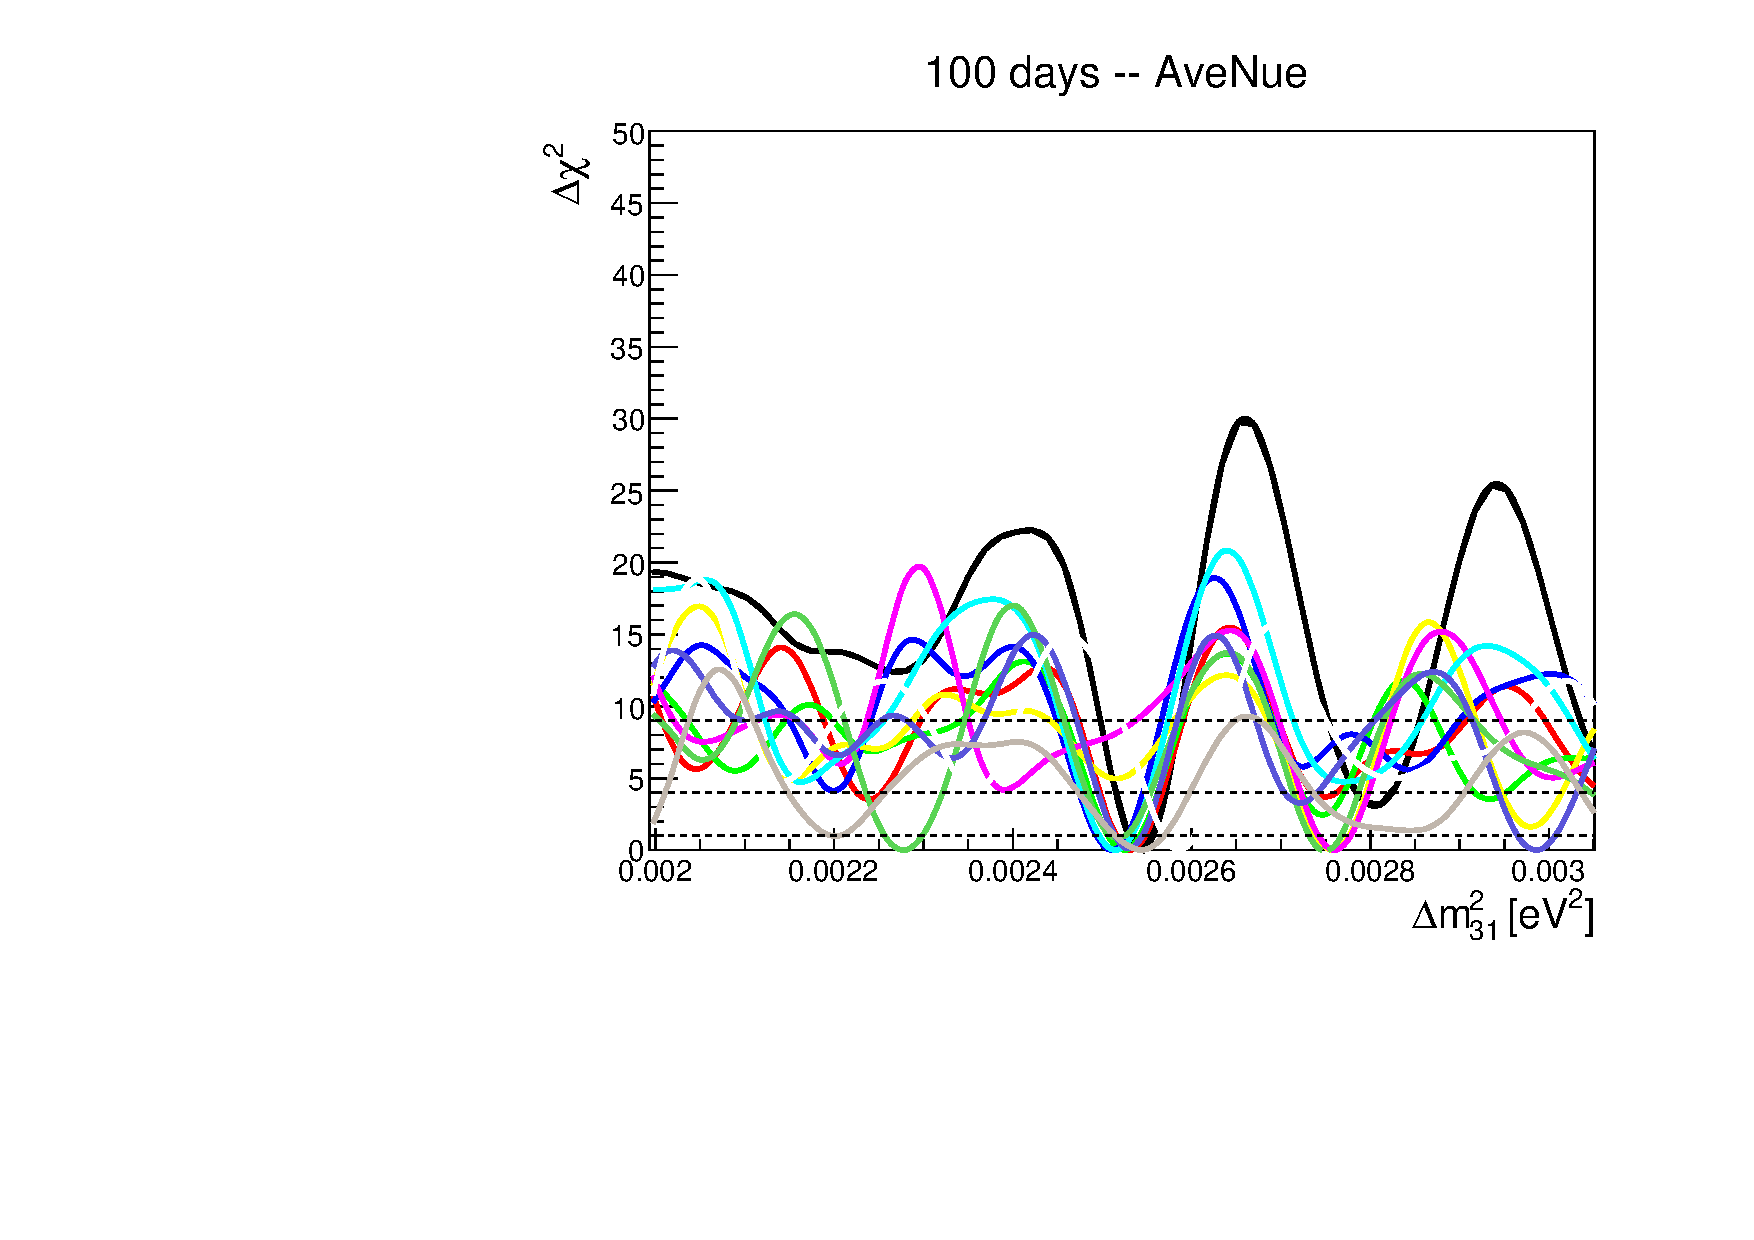
\includegraphics[width=\textwidth]{figs/Section2/benoitsteven_Prof_100d.pdf}
    \caption{ }
\end{subfigure}
\begin{subfigure}[b]{0.24\textwidth}
    \centering
    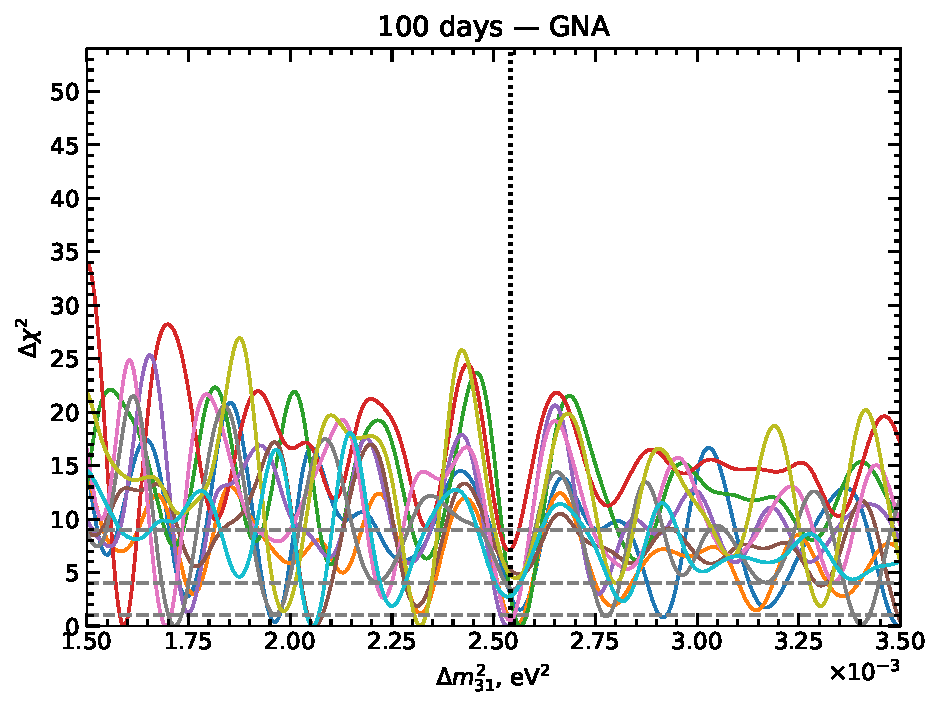
\includegraphics[width=\textwidth]{figs/Section2/dmitry_profiles_100d.pdf}
    \caption{ }
\end{subfigure} \\
% Row 3
\begin{subfigure}[b]{0.24\textwidth}
    \centering
    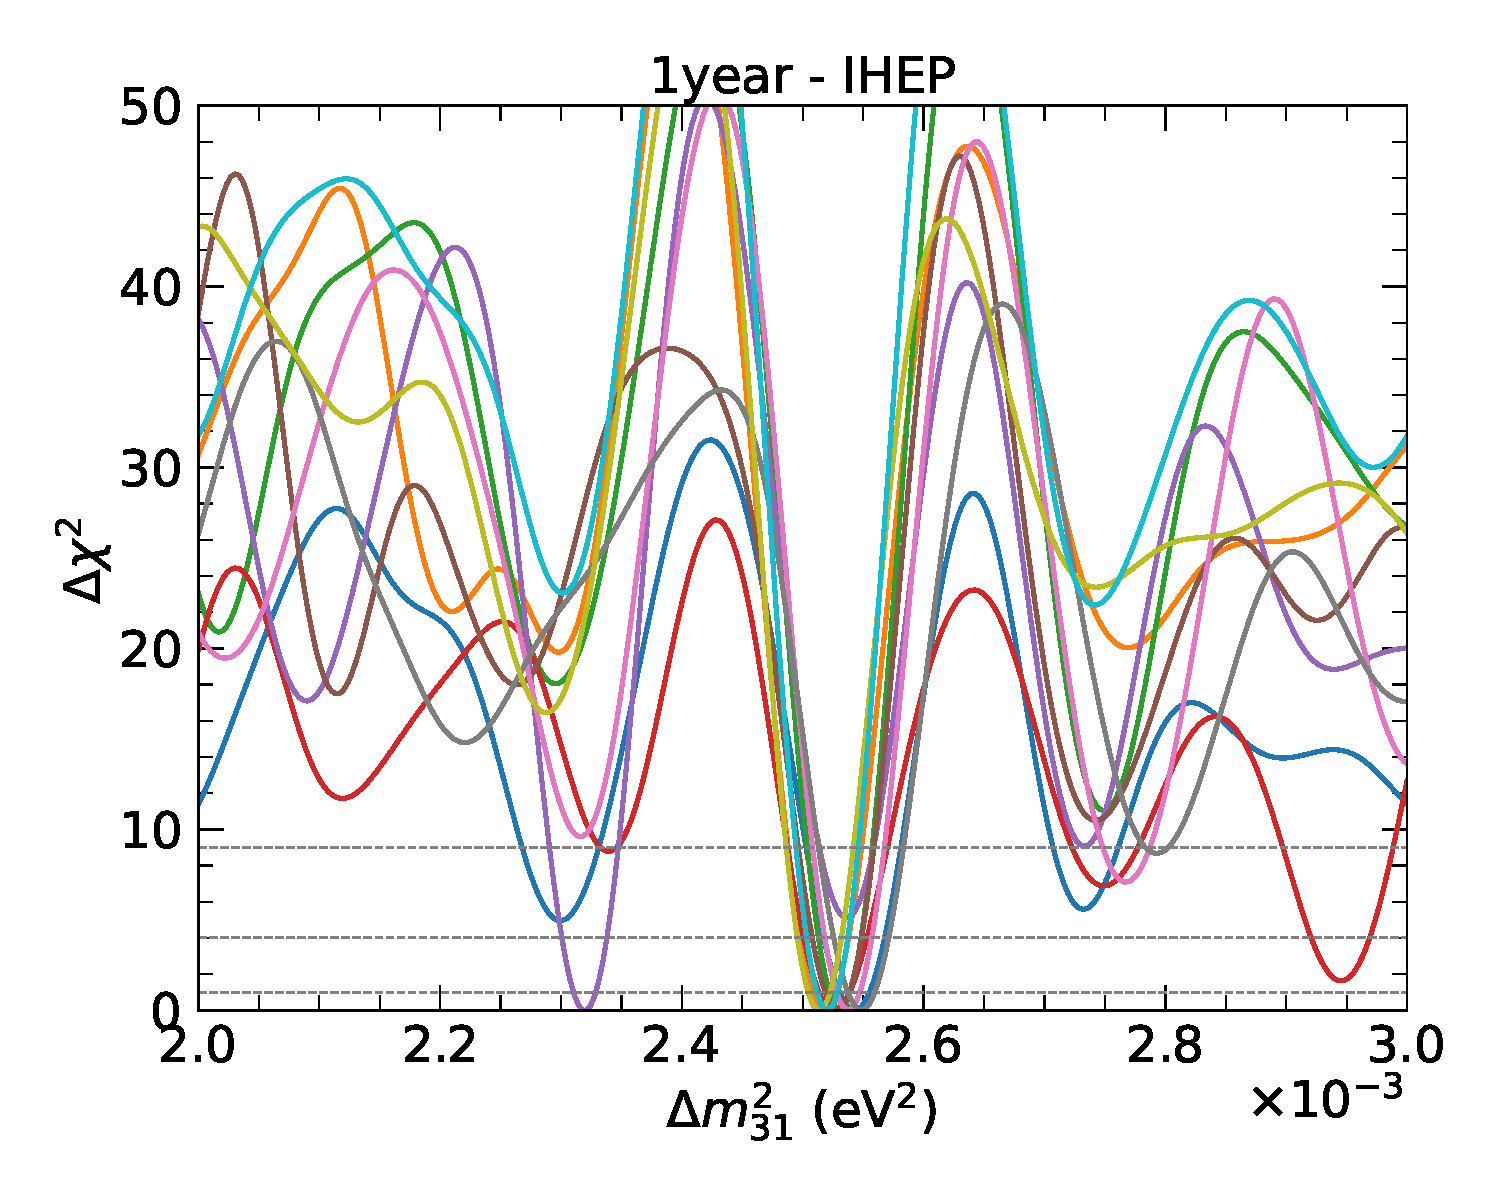
\includegraphics[width=\textwidth]{figs/Section2/Jingqin_1years_dmsq31_profile.pdf}
    \caption{ }
\end{subfigure} &
\begin{subfigure}[b]{0.24\textwidth}
    \centering
    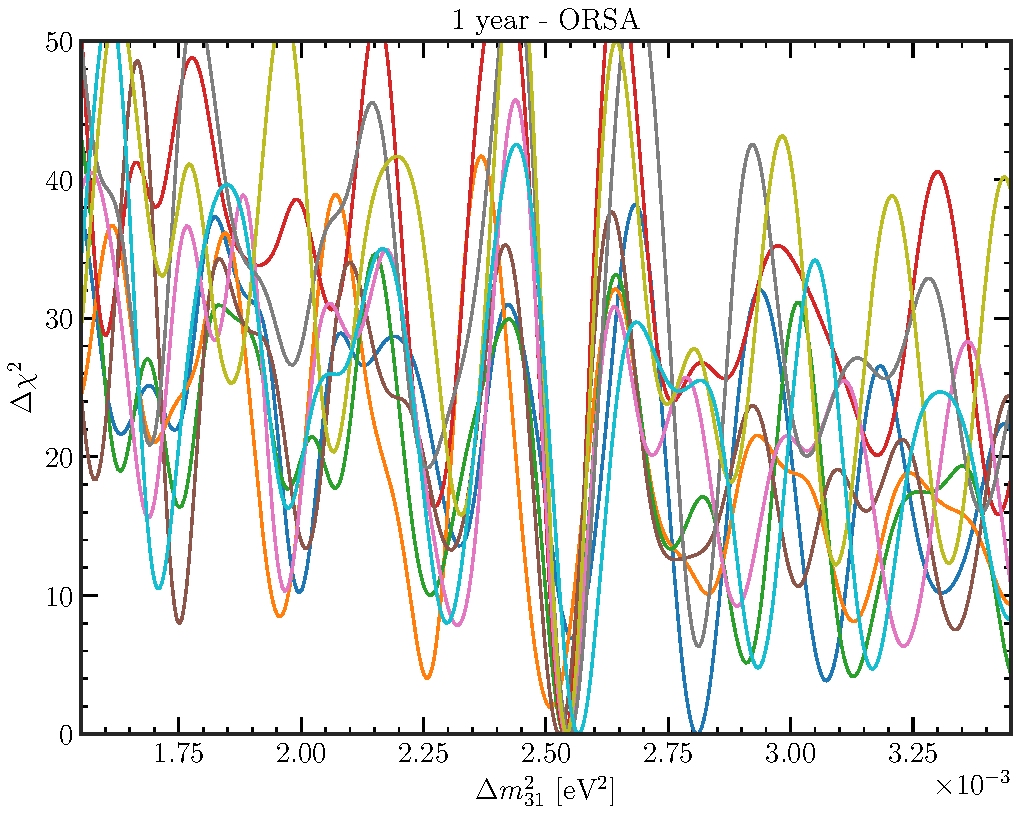
\includegraphics[width=0.94\textwidth]{figs/Section2/vanessa_profiles_1y.pdf}
    \caption{ }
\end{subfigure} &
\begin{subfigure}[b]{0.24\textwidth}
    \centering
    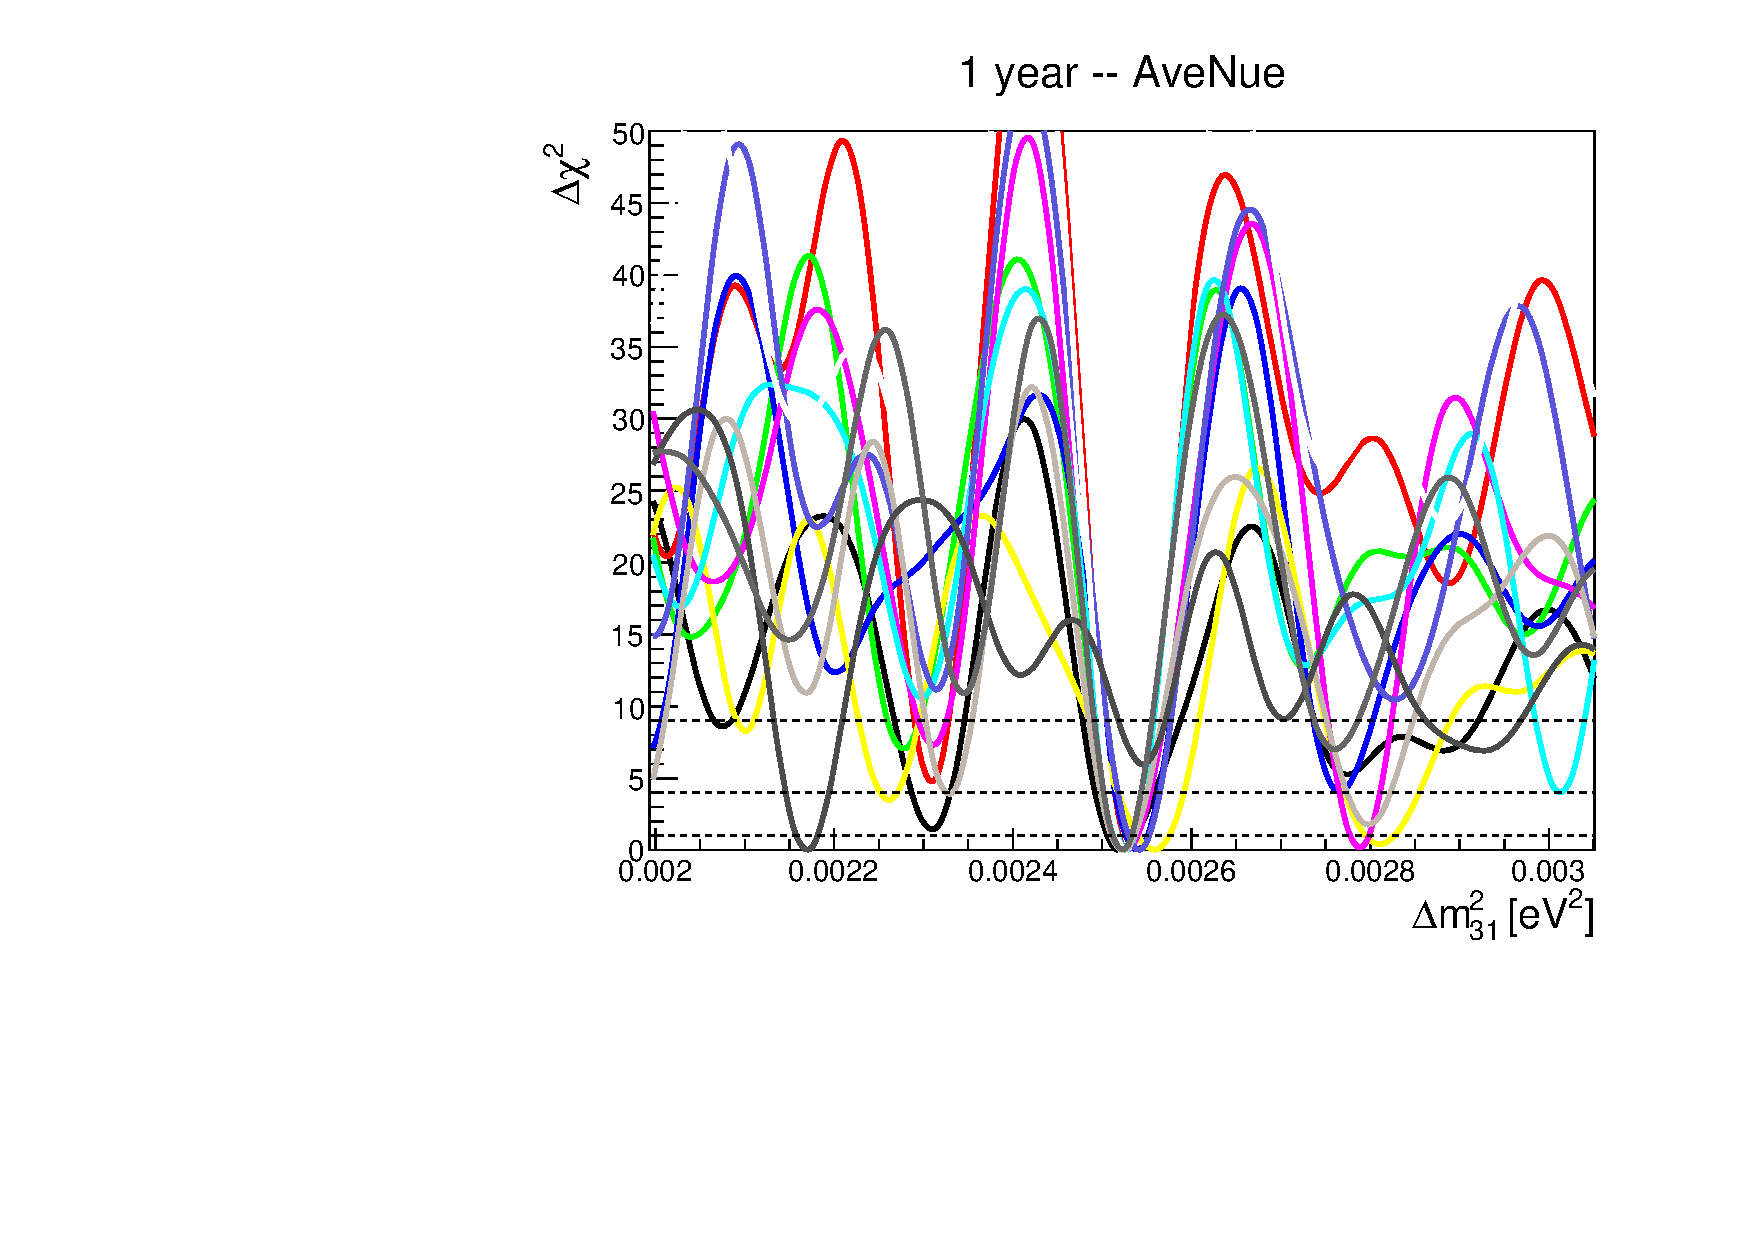
\includegraphics[width=\textwidth]{figs/Section2/benoitsteven_Prof_1yr.pdf}
    \caption{ }
\end{subfigure}
\begin{subfigure}[b]{0.24\textwidth}
    \centering
    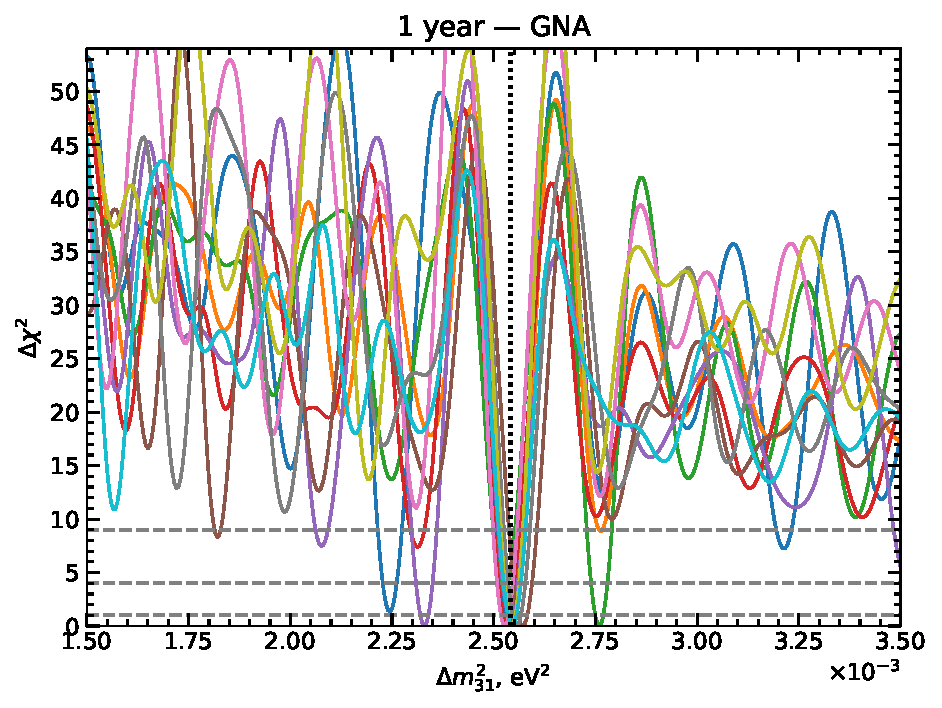
\includegraphics[width=\textwidth]{figs/Section2/dmitry_profiles_1y.pdf}
    \caption{ }
\end{subfigure} \\
% Row 4
\begin{subfigure}[b]{0.24\textwidth}
    \centering
    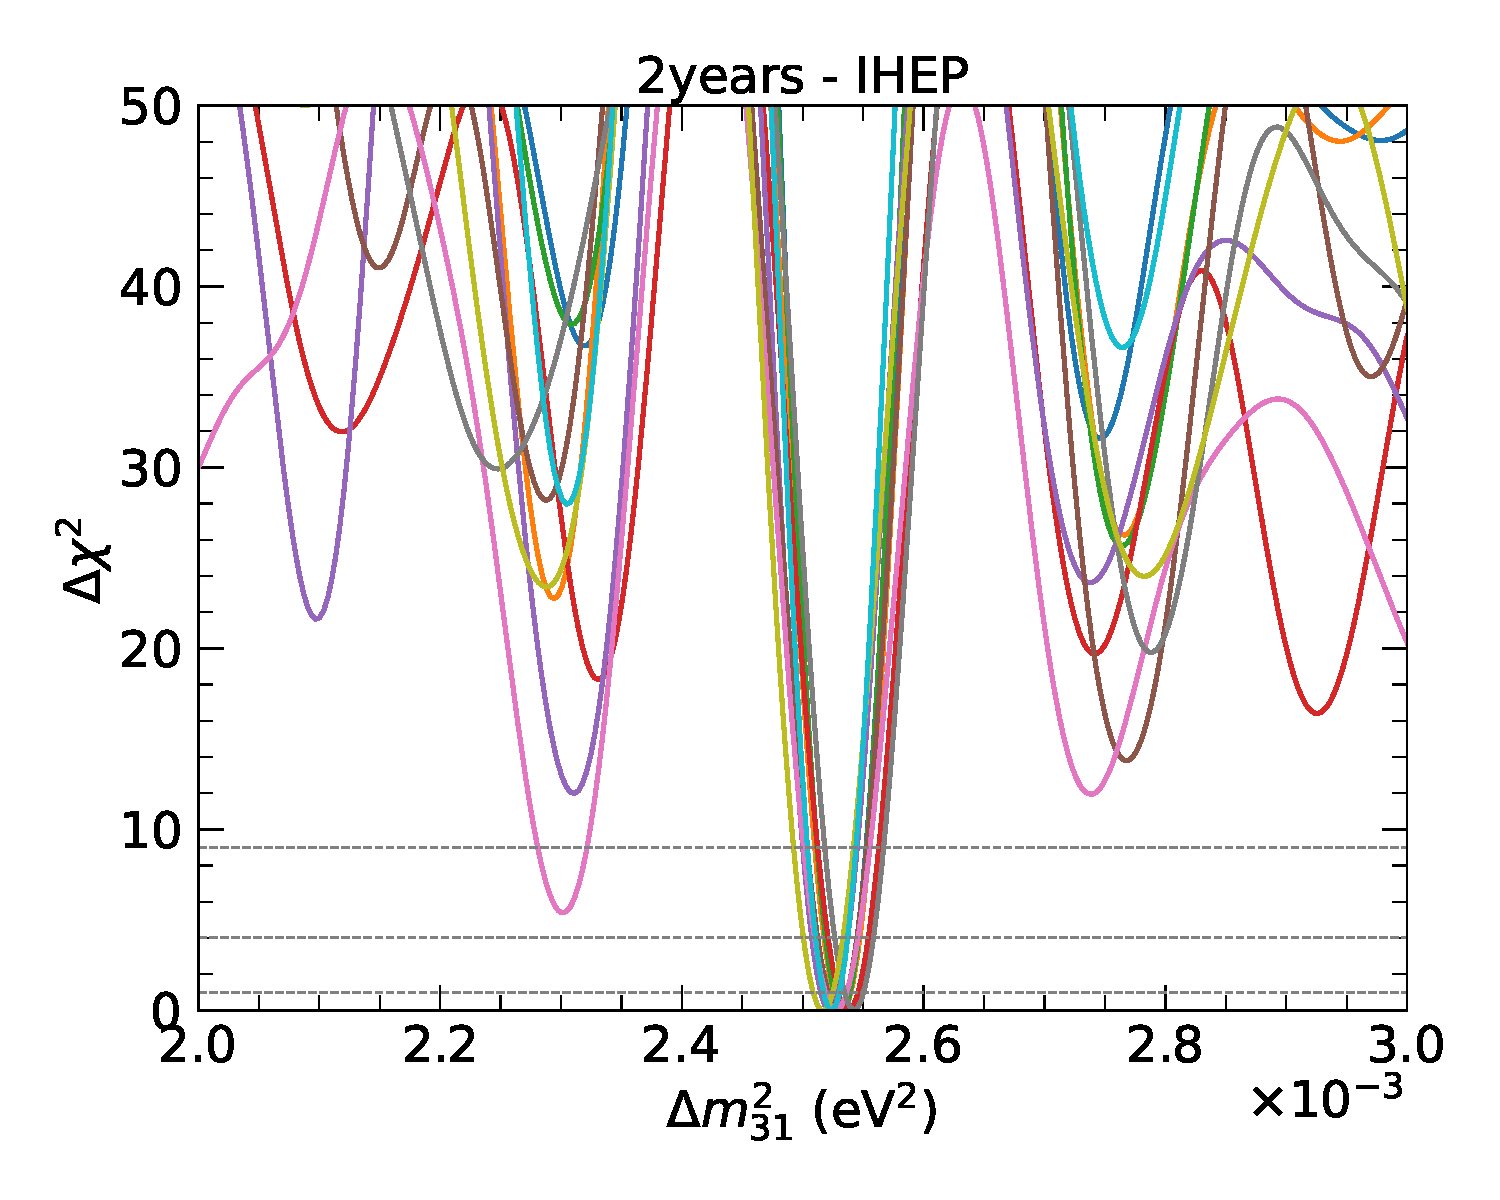
\includegraphics[width=\textwidth]{figs/Section2/Jingqin_2years_dmsq31_profile.pdf}
    \caption{ }
\end{subfigure} &
\begin{subfigure}[b]{0.24\textwidth}
    \centering
    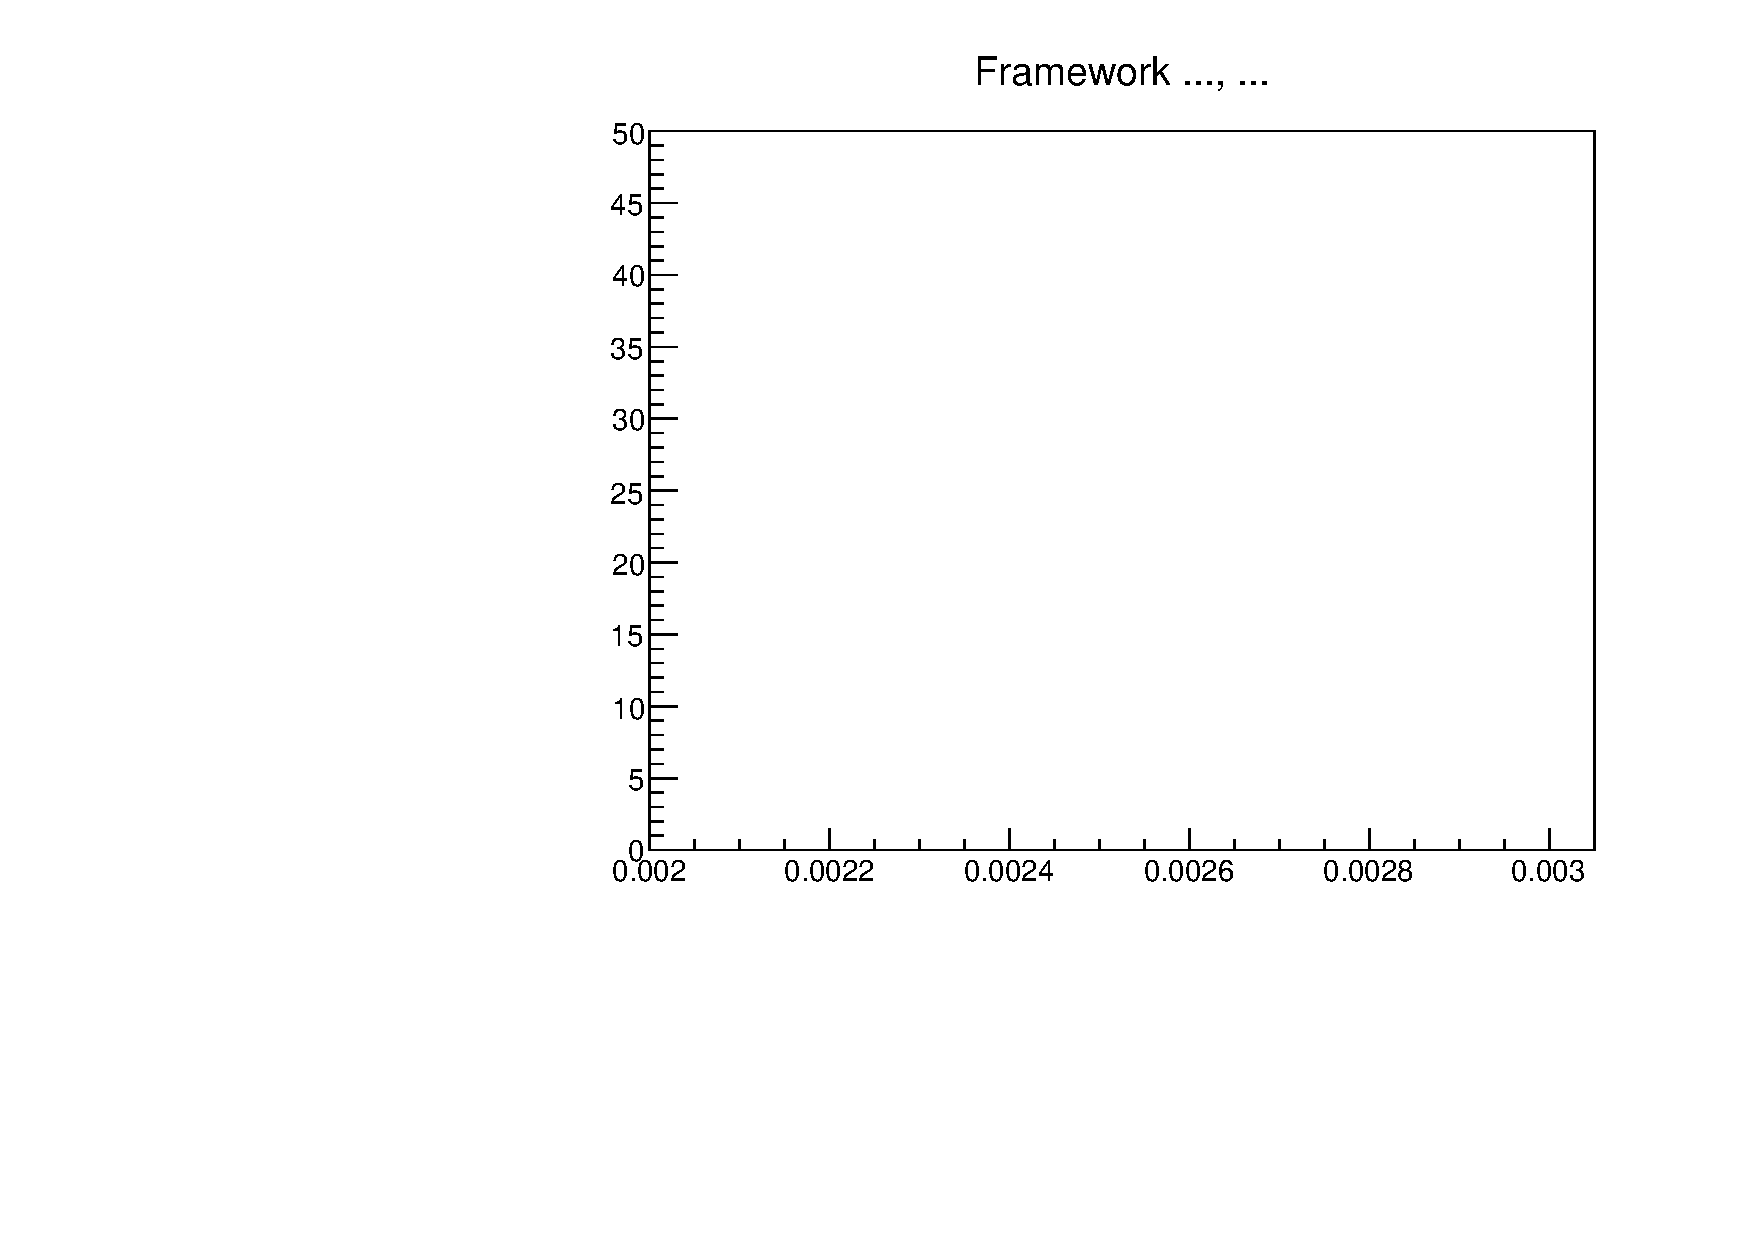
\includegraphics[width=\textwidth]{figs/Section2/benoitsteven_Prof_Generic.pdf}
    \caption{ }
\end{subfigure} &
\begin{subfigure}[b]{0.24\textwidth}
    \centering
    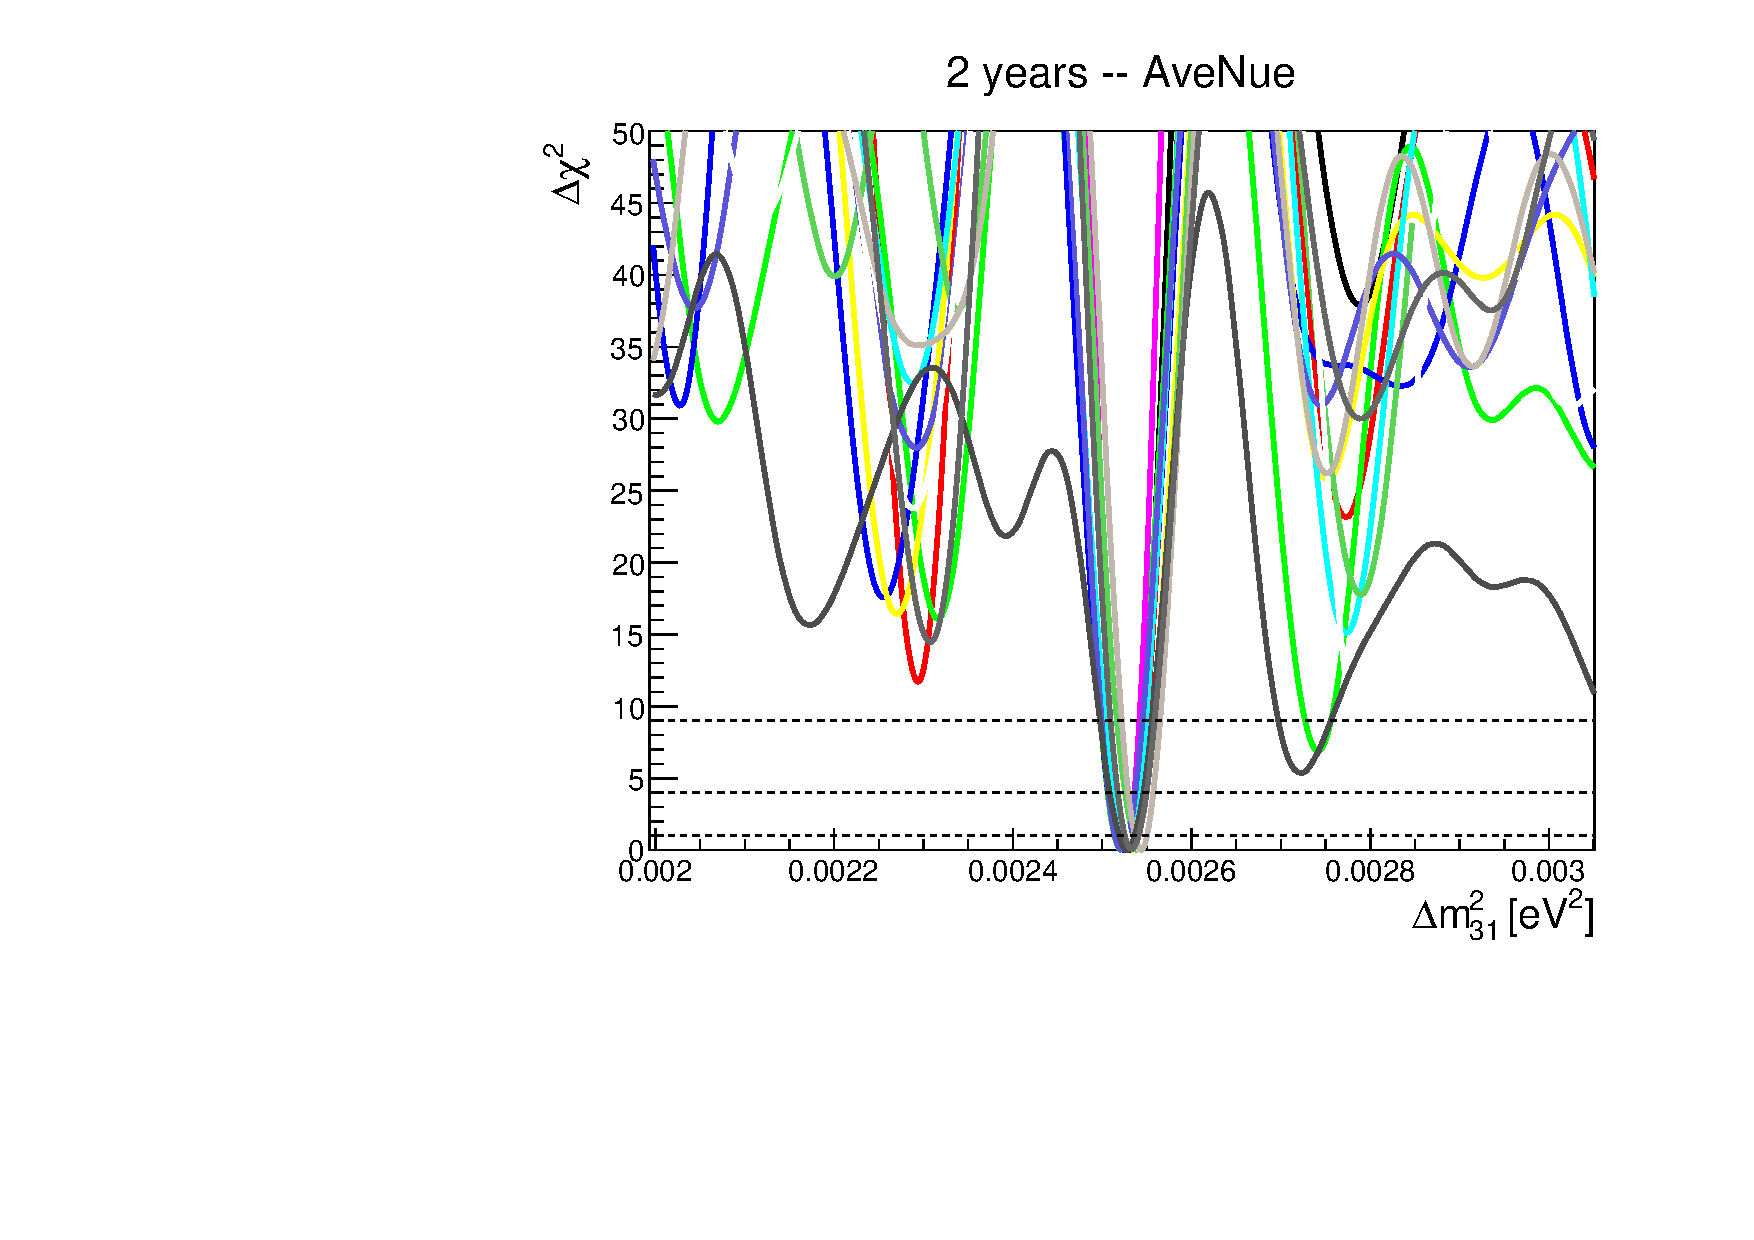
\includegraphics[width=\textwidth]{figs/Section2/benoitsteven_Prof_2yrs.pdf}
    \caption{ }
\end{subfigure}
\begin{subfigure}[b]{0.24\textwidth}
    \centering
    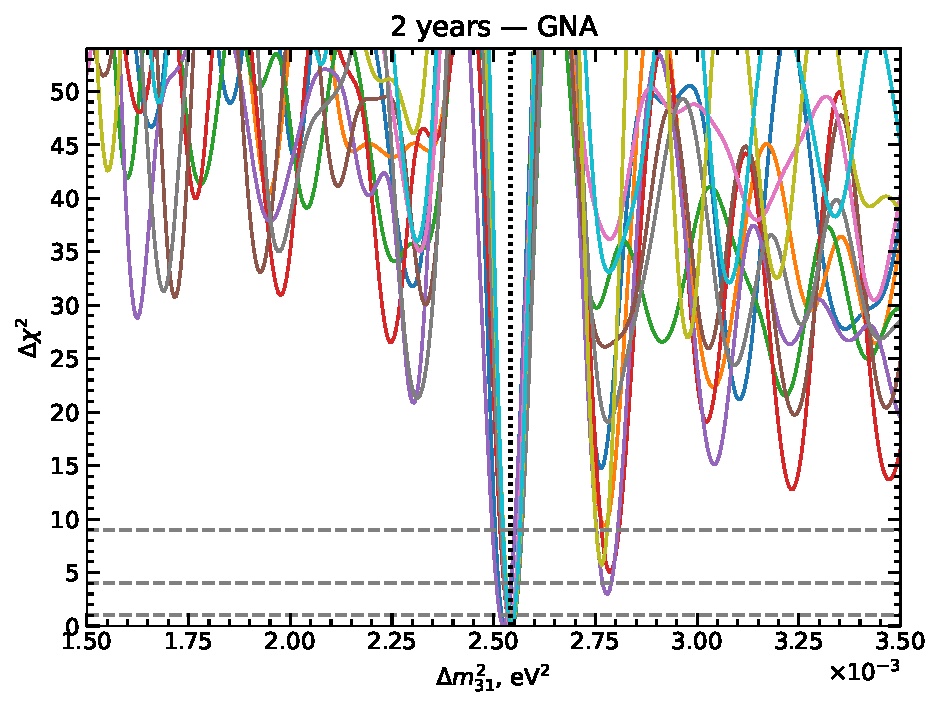
\includegraphics[width=\textwidth]{figs/Section2/dmitry_profiles_2y.pdf}
    \caption{ }
\end{subfigure} \\
% Row 5
\begin{subfigure}[b]{0.24\textwidth}
    \centering
    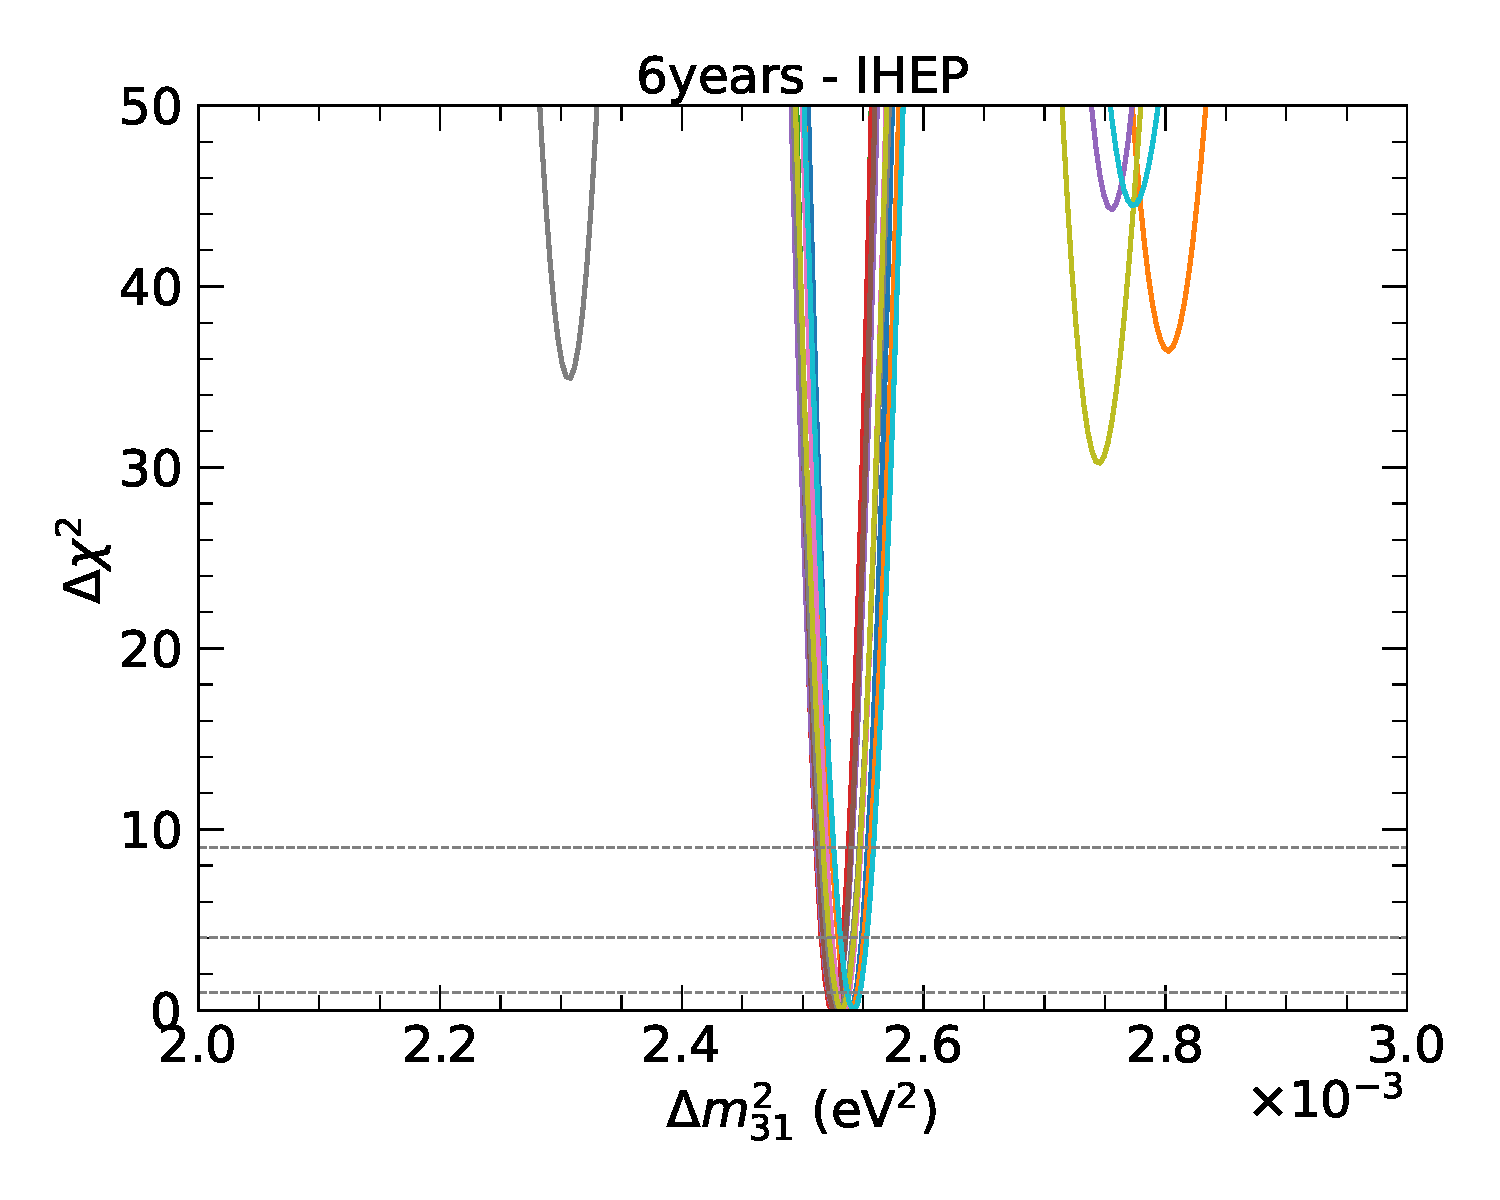
\includegraphics[width=\textwidth]{figs/Section2/Jingqin_6years_dmsq31_profile.pdf}
    \caption{ }
\end{subfigure} &
\begin{subfigure}[b]{0.24\textwidth}
    \centering
    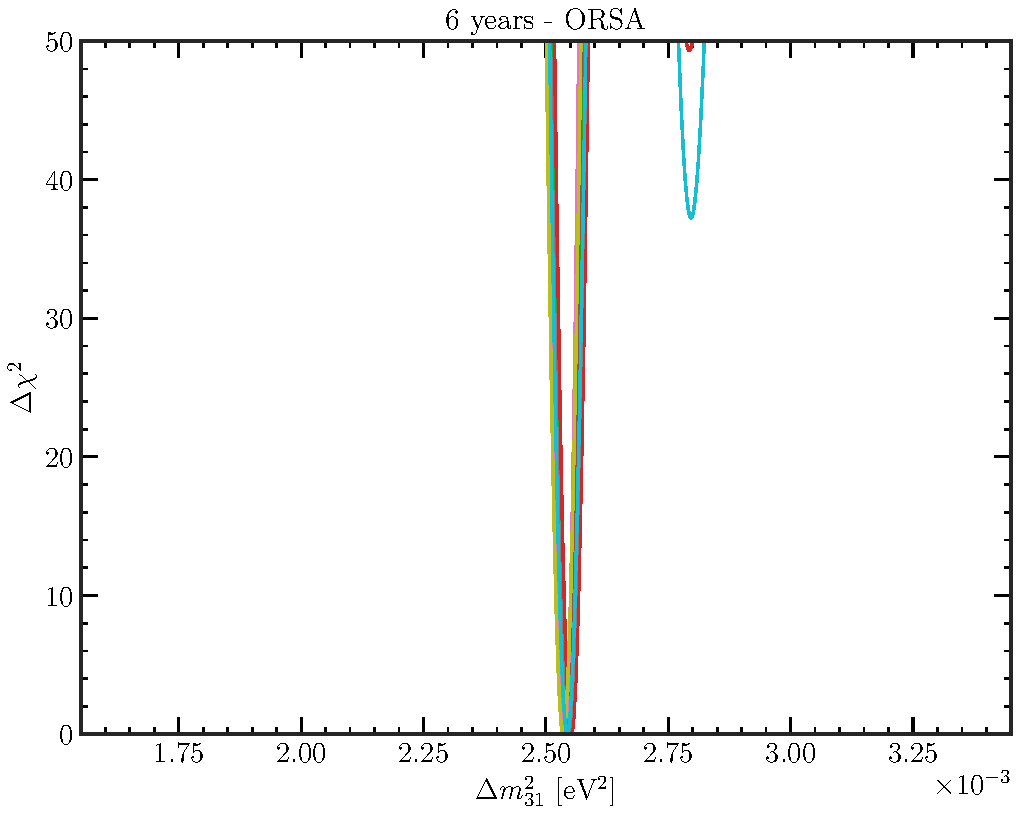
\includegraphics[width=0.94\textwidth]{figs/Section2/vanessa_profiles_6y.pdf}
    \caption{ }
\end{subfigure} &
\begin{subfigure}[b]{0.24\textwidth}
    \centering
    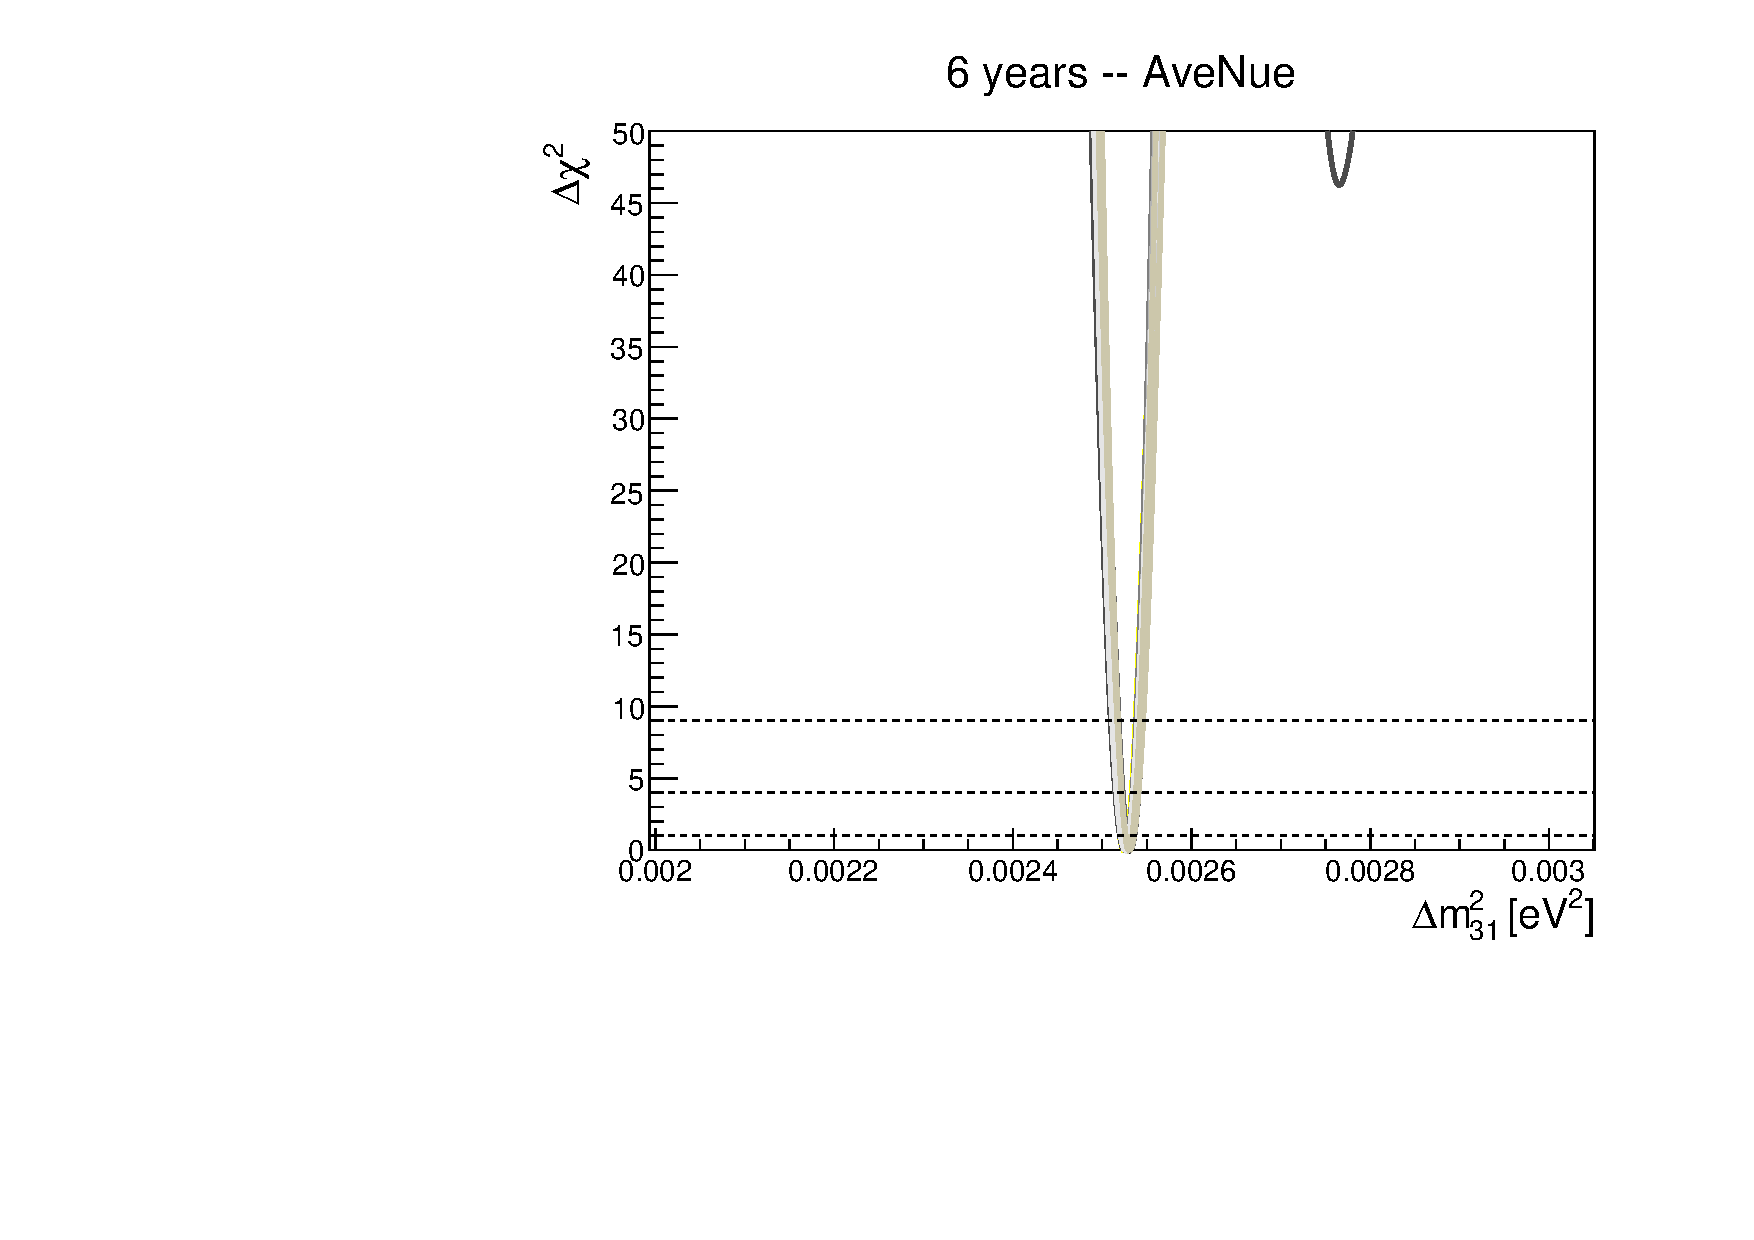
\includegraphics[width=\textwidth]{figs/Section2/benoitsteven_Prof_6yrs.pdf}
    \caption{ }
\end{subfigure}
\begin{subfigure}[b]{0.24\textwidth}
    \centering
    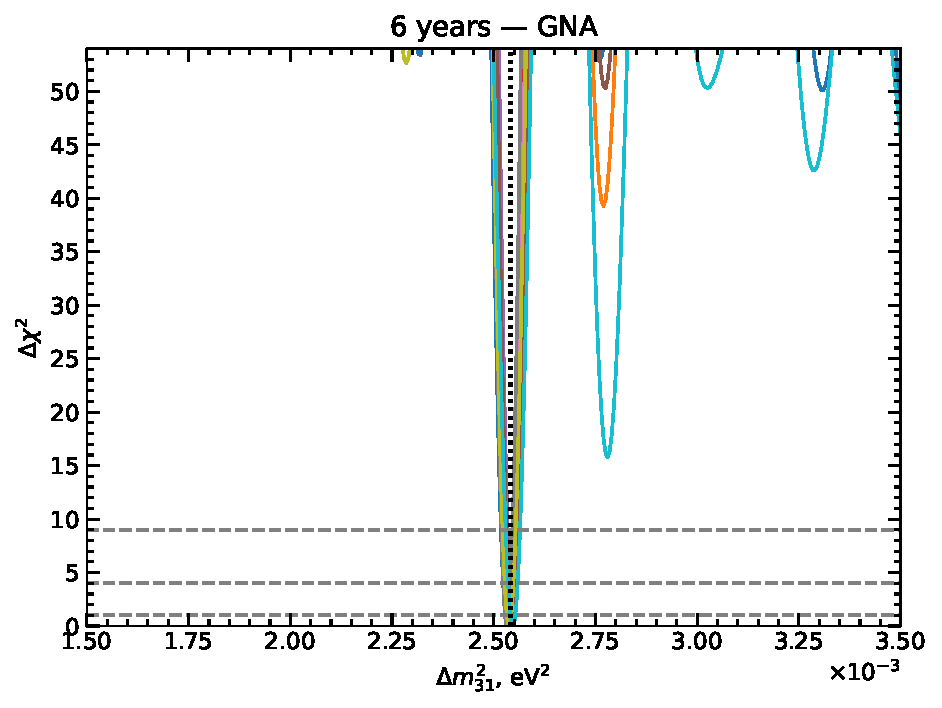
\includegraphics[width=\textwidth]{figs/Section2/dmitry_profiles_6y.pdf}
    \caption{ }
\end{subfigure} \\
\end{tabular}
\caption{$\chi^2$ profiles obtained by 4 frameworks, for 5 exposures}
\label{fig:mosaic}
\end{figure}

\end{comment}



\begin{table}[h!]
  \centering
  \caption{Key statistics quantifying the issues related to the measurement of $\Delta m^2_{32}$.}
  \label{tab:BadMinKeyStatistics}
  \vspace{10pt}
  %\begin{adjustbox}{angle=90} % Rotate the table by 30 degrees
    \begin{tabular}{|c|c|l|}
\hline
    Fractions of profiles                    &  Two or more disjointed       &  A single contiguous      \\ 
    resulting in                             &  CIs [$\%$]        &    CI [$\%$]              \\ 
\hline
 \multicolumn{3}{|c|}{50 days} \\
IHEP         &       47        &          37                    \\ \hline
ORSA        &         57       &        36                        \\ \hline
GNA          &       50         &  33                               \\ 
\hline

\multicolumn{3}{|c|}{100 days} \\
IHEP         &       35       &          26                    \\ \hline
ORSA        &          41      &        36                        \\ \hline
AveNue          &      31          &      33                          \\ \hline
GNA          &        35        &       31                          \\ 
\hline

\multicolumn{3}{|c|}{1 year} \\
IHEP         &       9        &              5                 \\ \hline
ORSA        &          10      &             12                   \\ \hline
AveNue          &      10         &          8                      \\ \hline
GNA          &        7        &           9                      \\ 
\hline


\multicolumn{3}{|c|}{6 years} \\
IHEP         &         0      &                 0             \\ \hline
ORSA        &          0       &               0               \\ \hline
AveNue          &      0          &             0                    \\ \hline
GNA          &         0        &              0                    \\ 
\hline

%      
    \end{tabular}
  %\end{adjustbox}$\Delta m^2_{31}$
\end{table}



\begin{comment}

\begin{table}[h!]
  \centering
  \caption{Key statistics quantifying the issues related to the measurement of $\Delta m^2_{32}$.}
  \label{tab:BadMinKeyStatistics}
  \vspace{10pt}
  %\begin{adjustbox}{angle=90} % Rotate the table by 30 degrees
    \begin{tabular}{|c|c|l|}
\hline
    Fractions of profiles                    &  A disjoint       &  A single contiguous      \\ 
    resulting in                             &  CI [$\%$]        &    CI [$\%$]              \\ 
\hline
 \multicolumn{3}{|c|}{50 days} \\
Framework 1         &                &                                \\ \hline
ORSA        &         57.4       &        36.1                        \\ \hline
AvenNue          &                &                                 \\ \hline
GNA          &       49.5         &  33.4                               \\ 
\hline

\multicolumn{3}{|c|}{100 days} \\
Framework 1         &                &                                \\ \hline
ORSA        &          41.4      &        36.5                        \\ \hline
AveNue          &      31          &      33                          \\ \hline
GNA          &        35.5        &       31.1                          \\ 
\hline

\multicolumn{3}{|c|}{1 year} \\
Framework 1         &                &                                \\ \hline
ORSA        &          9.6      &             11.5                   \\ \hline
AveNue          &      10         &          8                      \\ \hline
GNA          &        7.2        &           9.3                      \\ 
\hline

\multicolumn{3}{|c|}{2 years} \\
Framework 1         &                &                                \\ \hline
ORSA        &                &                                \\ \hline
AveNue          &                &                                 \\ \hline
GNA          &       1.0         &          1.8                       \\ 
\hline


\multicolumn{3}{|c|}{6 years} \\
Framework 1         &                &                                \\ \hline
ORSA        &         0.0       &               0.005               \\ \hline
AveNue          &      0          &             0                    \\ \hline
GNA          &        0.0        &             0.000                    \\ 
\hline

%      
    \end{tabular}
  %\end{adjustbox}$\Delta m^2_{31}$
\end{table}    
\end{comment}





%\begin{itemize}
%    \item Generic description : Several groups generated and fitted (see Section XX and App YY) thousands of toy
%   samples including fluctuations due both to statistical and syst effects ; produced thousands of realistics profiles.
%    \item Results
%    \begin{itemize}
%        \item One plot per analysis group,  showing a dozen typical  $\Delta m^2_{31}$ profiles superimposed.
%        \item Repeated for 5 exposures : 50 days, 100 days, 1 yr, 2 yrs, 6yrs.
%        \item Table: for each group and exposure: percentage of toys where there are several
%         minima ; percentage where the absolute minimum is far from the generation value (or any
%	    other metrics summarizing the problem).
%    \end{itemize}
%    \item Discussion $\&$ Conclusion
%    \begin{itemize}
%        \item Until a certain exposure : high risk to produce only a disjoint confidence interval (therefore a result far more uncertain than Asimov predictions),
%        not always containing the true value.
%        \item Until a certain exposure, Wilks theorem cannot be used.
%        \item This triggers the questions -- explored in the rest of the document -- on how to measure this exactly (statistical techniques ? external constraints ? ...)
%    \end{itemize}
%\end{itemize}

\section{Coverage}\label{sec:coverage}
% \begin{itemize}
%     \item Linked to previous section: the same toys (or procedure to generate toys) are used to study coverage properties.
% \end{itemize}

This section examines the coverage properties of confidence intervals using either the same simulated datasets from previous sections or datasets generated through a similar procedure. Specifically, we assess how effectively different methods for constructing confidence intervals achieve their intended nominal coverage levels.

\clearpage
\subsection{Wilks' theorem}
% \begin{itemize}
%     \item Outline assumptions of Wilks' theorem and why they are violated. Anticipate (or show with a plot) that we get undercoverage with Wilks' theorem. (comparison plots between Wilks and FC might be shown in the following subsection?)
% \end{itemize}
Wilks' theorem~\cite{Wilks:1938dza} provides an approximation to construct confidence intervals using the log-likelihood ratio test statistic. The theorem states that under certain regularity conditions, the test statistic 
\begin{equation}\label{eq:lambda_i}
\lambda_i = -2\log\frac{\mathcal{L}(\bm{x}|\theta_i, \hat{\hat{\bm \eta}})}{\mathcal{L}(\bm{x}|\hat{\theta}, \hat{\bm \eta})}
\end{equation}
asymptotically follows a $\chi^2$ distribution. Here, $\theta_i$ represents a specific test value for the parameter of interest $\theta$ (i.e., in this case, $\Delta m^2_{31}$, $\bm \eta$ represents a vector of nuisance parameters. 
The numerator is the likelihood evaluated at a specific test value $\theta_i$, with nuisance parameters optimized for that particular $\theta_i$ (indicate by the double-hat notation). The denominator is the maximum likelihood estimate, where both the parameter of interest and the nuisance parameters are simultaneously optimized (indicated by the single hat notation). For the construction of confidence intervals, this asymptotic behavior allows us to use tabulated critical values from the $\chi^2$ distribution to determine the boundaries of confidence regions. For 1 degree of freedom, the critical values are $\lambda = 1, 4, 9$ corresponding to 68.27\%, 95.45\%, and 99.73\% confidence levels, respectively.
Nevertheless, the validity of Wilks' theorem relies on several regularity conditions~\cite{Wilks:1938dza, Fan:2000gm, Cranmer:2005hi, Cowan:2010js, ParticleDataGroup:2024cfk}:

\begin{itemize}
    \item \textbf{Nested hypotheses}: the null hypothesis must be a special case of the alternative hypothesis, which is satisfied in parameter estimation problems where we test specific parameter values against the full parameter space.
    \item \textbf{Smoothness of the log-likelihood}: the log-likelihood function must be smooth (twice differentiable) with respect to the parameter $\theta$. This condition ensures that the estimators of the parameters follow ellipsoidal distributions~\cite{Fan:2000gm}, which is necessary for the asymptotic $\chi^2$ behavior.
    \item \textbf{Sample size}: The sample size must be large enough for the asymptotic approximation to be valid.
    %% there might be other conditions but I think these are enough to explain our specific case
\end{itemize}
Two of these assumptions are violated when estimating $\Delta m_{31}^2$ in JUNO at low exposure. Although the nested hypothesis condition holds when the parameter is constrained within a restricted interval, the most critical violation arises from the fact that the log-likelihood distribution does not have an ellipsoidal shape at low-stats (see \autoref{sec:2_bad_minima}, where the reported $\Delta \chi^2$ profiles are non-parabolic). As a consequence, since Wilks' theorem conditions are not satisfied, using tabulated critical values from the $\chi^2$ distribution leads to wrong confidence intervals and coverage properties. Specifically, we anticipate that for $\Delta m_{31}^2$, this produces undercoverage, where the actual coverage probability is found to be below the desired confidence level. 


\subsection{Feldman-Cousins approach}
To address these limitations, Feldman and Cousins~\cite{Feldman_1998} introduced a
confidence interval construction based on an ordering principle derived from the 
likelihood ratio. The main idea behind the Feldman-Cousins (FC) method is to 
empirically determine the correct critical values by generating pseudoexperiments. 
This approach does not rely on any approximation and should yield accurate 
confidence intervals even when the likelihood does not follow a $\chi^2$ 
distribution. Nevertheless, the original FC method was designed for simple cases 
without nuisance parameters and their presence would complicate the procedure. To 
address this, we implement the Profiled FC technique, following the approach 
developed and validated by the NO$\nu$A collaboration~\cite{NOvA:2022wnj}. The procedure consists of the following steps:

\begin{enumerate}
    \item A sufficiently fine grid of $\theta_i$ values is defined across the parameter space of interest for $\Delta m_{31}^2$, serving as input for generating pseudo-experiments. In most of the cases discussed below, we use a grid of 80 equally spaced points spanning the range $\theta_i \in [1.5, 3.5]$ eV$^2$.
    \item For each grid point $\theta_i$, the nuisance parameters $\bm{\eta}$ are 
    set to their profiled values\footnote{When real data is available, this 
    profiling procedure involves fitting the real data with the parameter of 
    interest $\theta$ fixed at each grid point $\theta_i$ and finding the nuisance 
    parameters $\hat{\hat{\bm{\eta}}}_i$ that minimize the cost function (or 
    equivalently, maximize the likelihood) at that grid point. However, since we 
    do not have real data available for this study, we use the Asimov dataset with 
    nominal parameter values as a proxy for real data. } 
    $\hat{\hat{\bm{\eta}}}_i$, which are the values that maximize the likelihood 
    for that $\theta_i$. This procedure gives a set of $(\theta_i, 
    \hat{\hat{\bm{\eta}}}_i)$ pairs which should be used as input values to 
    generate FC toy experiments.
    \item For each grid point $(\theta_i, \hat{\hat{\bm{\eta}}}_i)$, $N=5000$ toy experiments, denoted as $t_{ij}$ where $j = 1 \ldots N$, are generated. These toy experiments include both statistical and systematic fluctuations, as described in \autoref{appendix:pseudoexp}.
    \item For each $t_{ij}$, we perform a fit and obtain the $\chi^2$ profile for $\Delta m_{31}^2$. The test statistic introduce in \autoref{eq:lambda_i} is then calculated as:
    \begin{equation}\label{eq:lambda_ij_FC_chi2}
        \lambda_{ij} = \chi^2(t_{ij}|\theta_i, \hat{\hat{\bm{\eta}}}_{ij}) - \chi^2(t_{ij}|\hat{\theta}_j, \hat{\bm{\eta}}_j)
    \end{equation}
    where:
    \begin{itemize}
        \item[-] $\chi^2(t_{ij}|\theta_i, \hat{\hat{\bm{\eta}_{ij}}})$ is the $\chi^2$ profile evaluated at the fixed value $\theta_i$ with nuisance parameters profiled for that specific toy.
        \item[-] $\chi^2(t_{ij}|\hat{\theta}_j, \hat{\bm{\eta}}_j)$ is the $\chi^2$ profile evaluated at the global minimum, with $(\hat{\theta}_j, \hat{\bm{\eta}}_j)$ representing the best fit values for all parameters.
    \end{itemize}
\autoref{fig:teststat_FC_profile} shows the $\chi^2$ profile for a single pseudoexperiment $t_{ij}$, where the blue curve represents the full profile, the purple star indicates $\chi^2(t_{ij}|\theta_i, \hat{\hat{\bm{\eta}_{ij}}})$, and the green star shows $\chi^2(t_{ij}|\hat{\theta}_j, \hat{\bm{\eta}}_j)$ at the global minimum. The test statistic $\lambda{ij}$ is calculated as the difference between these two values.
\item The distribution of $\lambda_{ij}$ values from all toy experiments at point $\theta_i$ provides the empirical probability density function, denoted as $P(\lambda_i)$.  Following the FC ordering rule, the $\lambda_{ij}$ values are sorted in ascending order to determine the critical value $c_{\alpha,i}$\footnote{The notation $\Delta \chi^2_{\rm crit}$ is also used to indicate the critical value.} such that:
\begin{equation}\label{eq:FC_integral}
\int_0^{c_{\alpha,i}} P(\lambda_i) d\lambda_i = \alpha
\end{equation}
for the $\alpha$-level confidence interval\footnote{Following the NO$\nu$A collaboration's convention~\cite{NOvA:2022wnj}, $\alpha$ in~\autoref{eq:FC_integral} represents the confidence level directly (e.g., $\alpha = 0.6827$ for 68.27\% CL), rather than the traditional statistical notation~\cite{Feldman_1998} where $\alpha$ typically denotes the significance level and the integral would be defined as $(1-\alpha)$. This notation simplifies the implementation since $\alpha$ directly corresponds to the desired coverage probability without requiring additional transformations.}. This procedure is repeated for all 
grid points $\theta_i$ to obtain a complete set of critical values $c_{\alpha,i}$.
The confidence interval is then constructed by including all parameter values 
$\theta_i$ for which the observed test statistic falls below the corresponding 
critical value $c_{\alpha,i}$. \autoref{fig:empirical_test_stat} displays the 
empirical distribution of $\lambda_{ij}$ values obtained from $N$ toy experiments. 
The vertical black dashed line indicates the critical value corresponding to 68.27\% 
confidence level. For comparison, both the 1 dof $\chi^2$ theoretical distribution and the corresponding critical value for 68.27\%  (i.e., $\lambda = 1$) are reported. The critical value obtained with FC is higher than what we would get with Wilks' theorem, anticipating possible undercoverage.
\end{enumerate}

\begin{figure}[ht]
  \centering
  \begin{subfigure}[t]{0.49\textwidth}
    \centering
    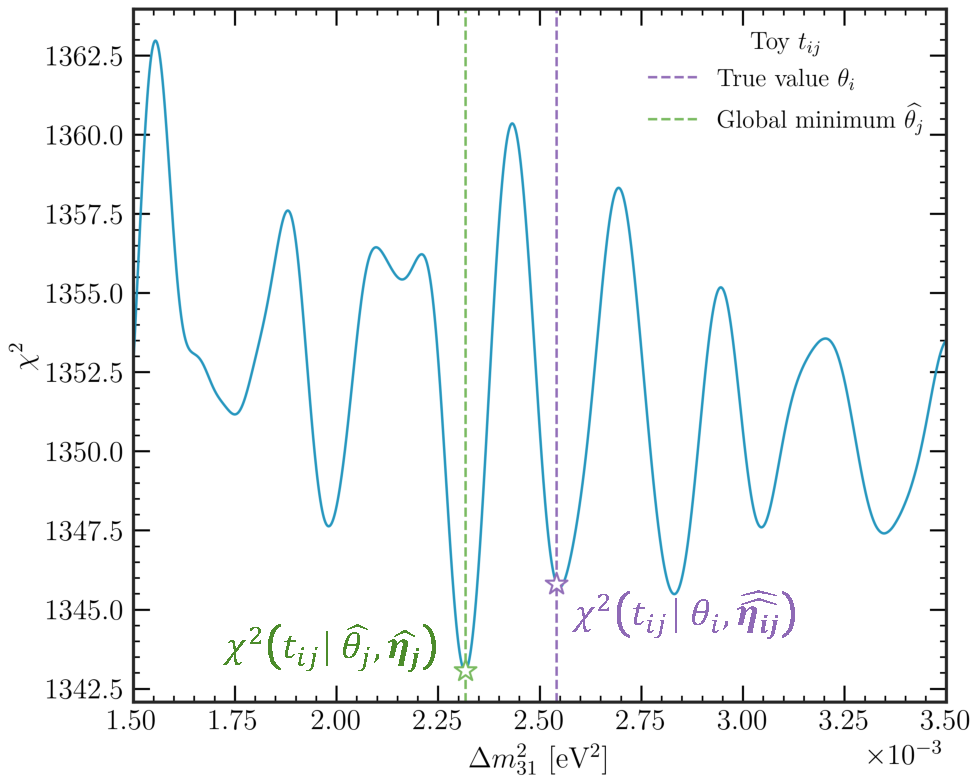
\includegraphics[width=\linewidth]{figs/Section2/vanessa_FC_teststatistics.pdf}
    \caption{$\chi^2$ profile for a single toy at $\theta_i = 0.00253$ eV$^2$.}
    \label{fig:teststat_FC_profile}
  \end{subfigure}
  \hfill
  \begin{subfigure}[t]{0.49\textwidth}
    \centering
    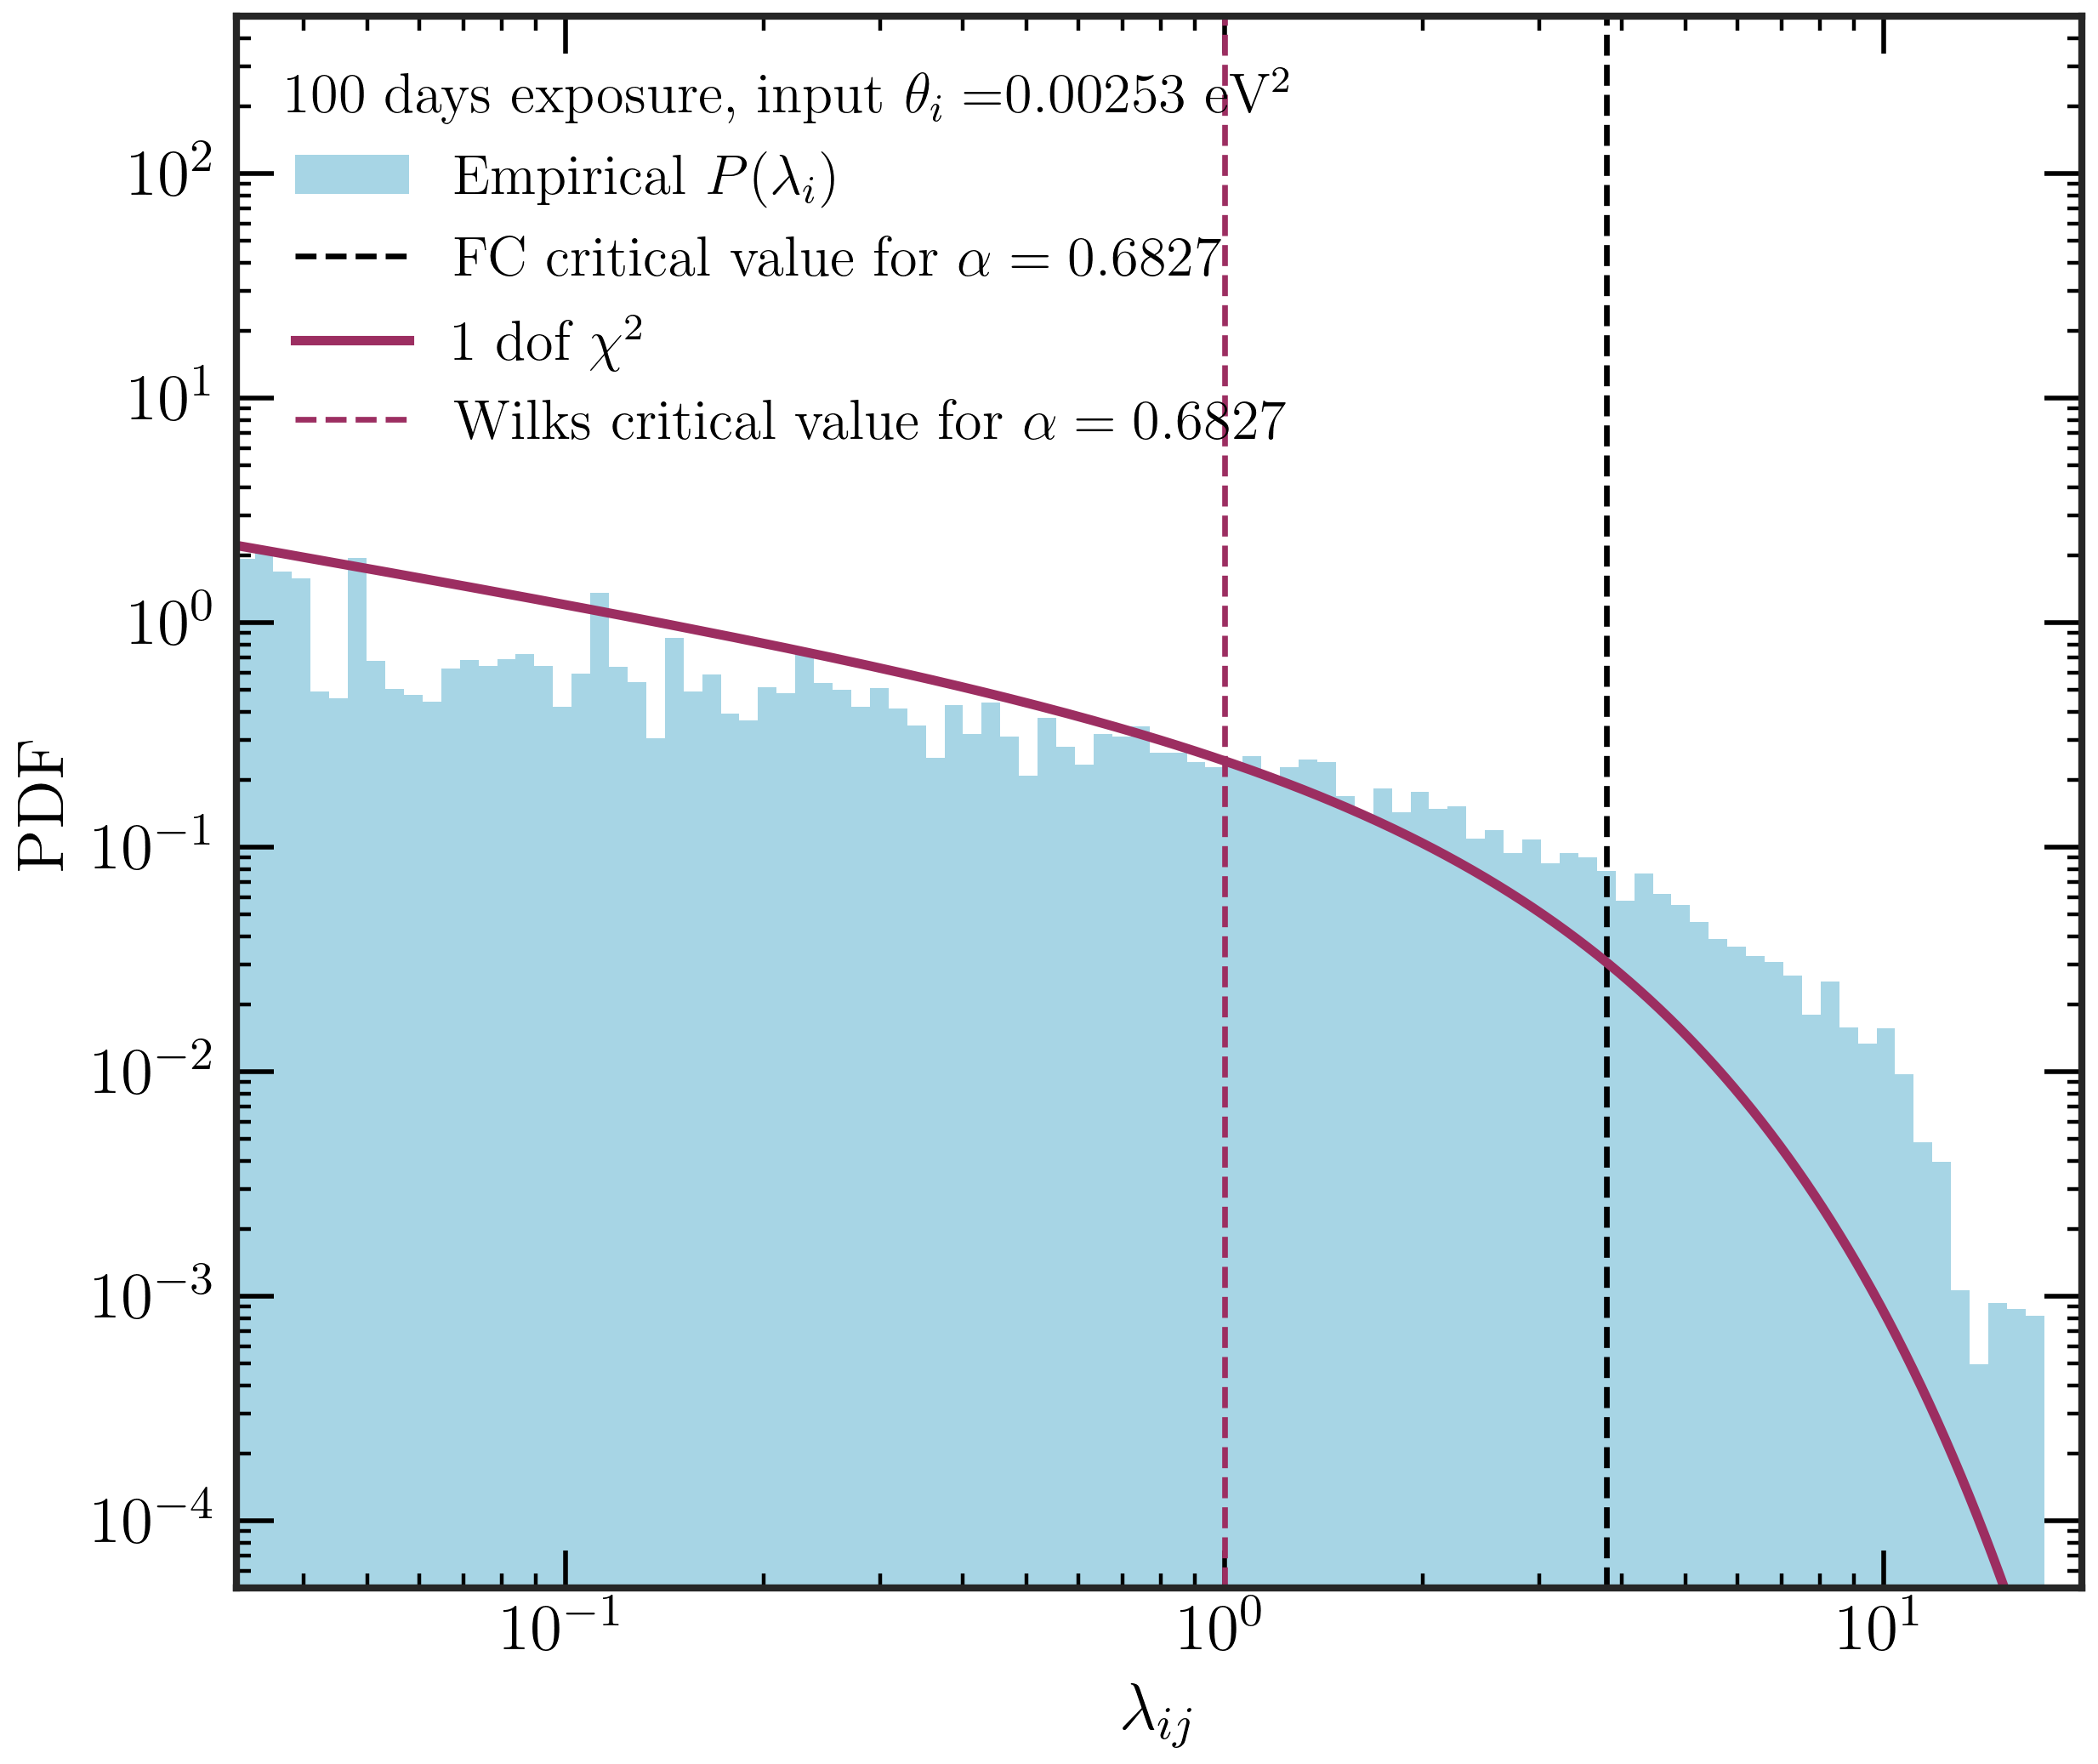
\includegraphics[width=0.96\linewidth]{figs/Section2/vanessa_100d_comparison_chi2_66_v2.png}
    \caption{Empirical distribution of test statistic $\lambda_{ij}$ from 5000 toys.}
    \label{fig:empirical_test_stat}
  \end{subfigure}
  \caption{Feldman-Cousins procedure for determining empirical critical values at 100 days exposure.}
  \label{fig:example_figs_FC}
\end{figure}

The FC technique was tested by two independent analyzers. The analyses mostly share the same inputs and assumptions, while the primary difference lies in the treatment of nuisance parameters:
\begin{itemize}
    \item Analyzer 1: This implementation follows the full profiled FC procedure, profiling the nuisance parameters at each grid point $\theta_i$. This ensures a thorough treatment of systematic uncertainties and properly captures correlations between parameters.
    \item Analyzer 2: This approach simplifies the process by fixing the nuisance parameters to their best-fit values $\hat{\bm{\eta}}_j$, rather than re-optimizing them for each $\theta_i$. In other words, it replaces $\hat{\hat{\bm{\eta}}}_{ij}$ with $\hat{\bm{\eta}}_j$, significantly reducing the computational load while still providing reasonably accurate results for $\Delta m_{31}^2$. This approximation is justified for these studies because $\Delta m_{31}^2$  is not heavily affected by systematic uncertainties. Still, the full profiling approach offers a more robust treatment of parameter correlations and is expected to be necessary for the final physics results, where systematics may play a more important role.
\end{itemize}

\subsubsection{Validation pseudoexperiments at 1 year exposure}
To evaluate coverage properties and compare confidence intervals derived from Wilks' theorem and the FC method, we generate 20,000 validation pseudoexperiments assuming a known true value $\theta = \theta_0$ and a 1-year exposure. Confidence intervals using Wilks' theorem are constructed based on critical values from the chi-square distribution with 1 degree of freedom, while FC intervals are built using the aforementioned construction procedure. Specifically, for each validation toy $t_k$, the log-likelihood ratio test statistic is calculated as \autoref{eq:lambda_ij_FC_chi2}, i.e, $\lambda_{ik} = \Delta\chi^2$. All points such that $\lambda_{ik} < c_{i,\alpha}$ belong to the confidence interval at significance level $\alpha$, where $c_{i,\alpha}$ are the critical values determined from the FC procedure. The true value $\theta_0$ is included in the confidence interval at significance level $\alpha$ if $\lambda_{0k} < c_{0,\alpha}$.
Following the approach of the NO$\nu$A collaboration~\cite{NOvA:2022wnj}, we assess the performance of both methods at various points in parameter space to verify that the empirically determined critical values provide correct frequentist coverage, independent of the true parameter value. 
\autoref{fig:FC_validation_1y} compares the coverage of the FC method (blue curves) and Wilks’ theorem (purple curves) across the tested values of $\theta_0$, i.e., $\theta_0 = \text{DYB} - 3\sigma$, $\theta_0 = \text{DYB}$ (recent Daya Bay value~\cite{DayaBay:2022orm}), and $\theta_0 = \text{DYB} + 3\sigma$, where DYB refers to the current best-fit value from Daya Bay. Additional tests are conducted at $\theta_0 = \text{DYB} \pm 5\sigma$ to probe the method's behavior near the edges of the physically meaningful parameter range. Similar results are obtained but not shown in this document. The intended coverage refers to the nominal confidence level used to define the critical values, while the effective coverage is the observed fraction of pseudoexperiments where the interval actually contains the true value. A method with perfect coverage yields effective coverage equal to the intended one, shown as the diagonal line in the plots. The results highlight several important findings:
\begin{itemize}
    \item By construction, the FC method achieves coverage that accurately follows the ideal diagonal (black dashed line) across all tested true values.
    \item Wilks' theorem consistently exhibits undercoverage, i.e., the purple curves systematically falls below the ideal coverage line. This undercoverage becomes increasingly pronounced at higher confidence levels, where the deviation from the asymptotic $\chi^2$ behavior is most significant.
\end{itemize}

\begin{figure}[ht]
  \centering
  \begin{subfigure}[t]{0.32\textwidth}
    \centering
    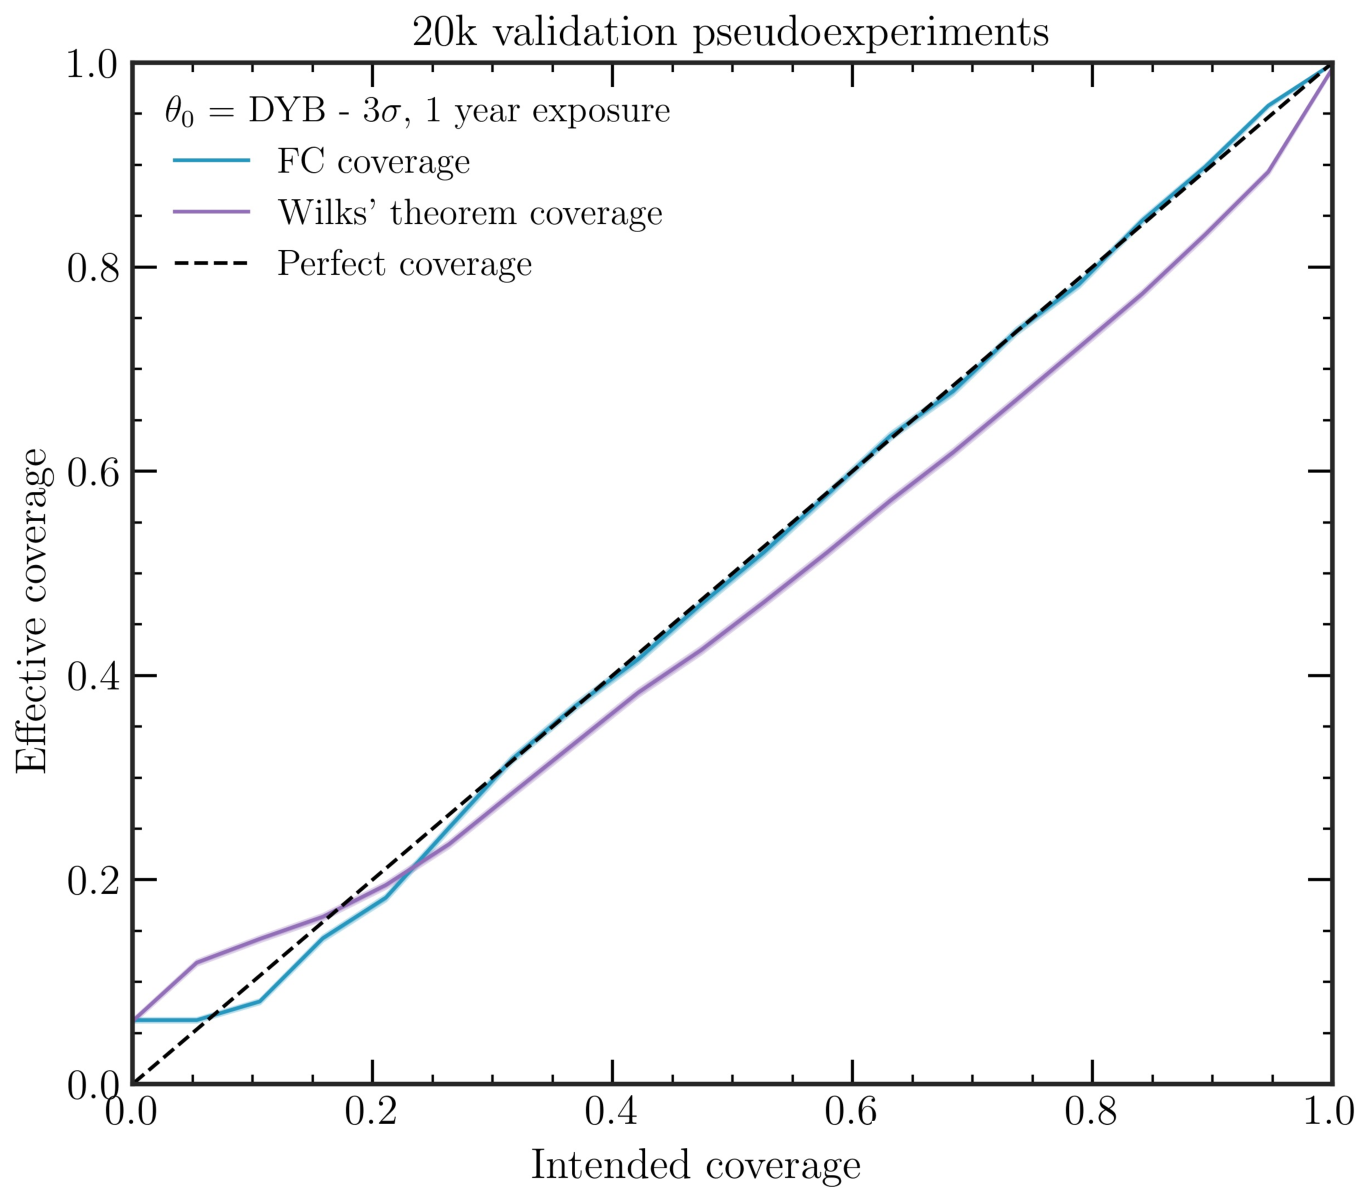
\includegraphics[width=\linewidth]{figs/Section2/vanessa_FC_1y_val_dybm3.png}
    \caption{$\theta_0 = \text{DYB} - 3\sigma$}
    \label{fig:FC_validation_DYBm3s_1y}
  \end{subfigure}
  \hfill
  \begin{subfigure}[t]{0.32\textwidth}
    \centering
    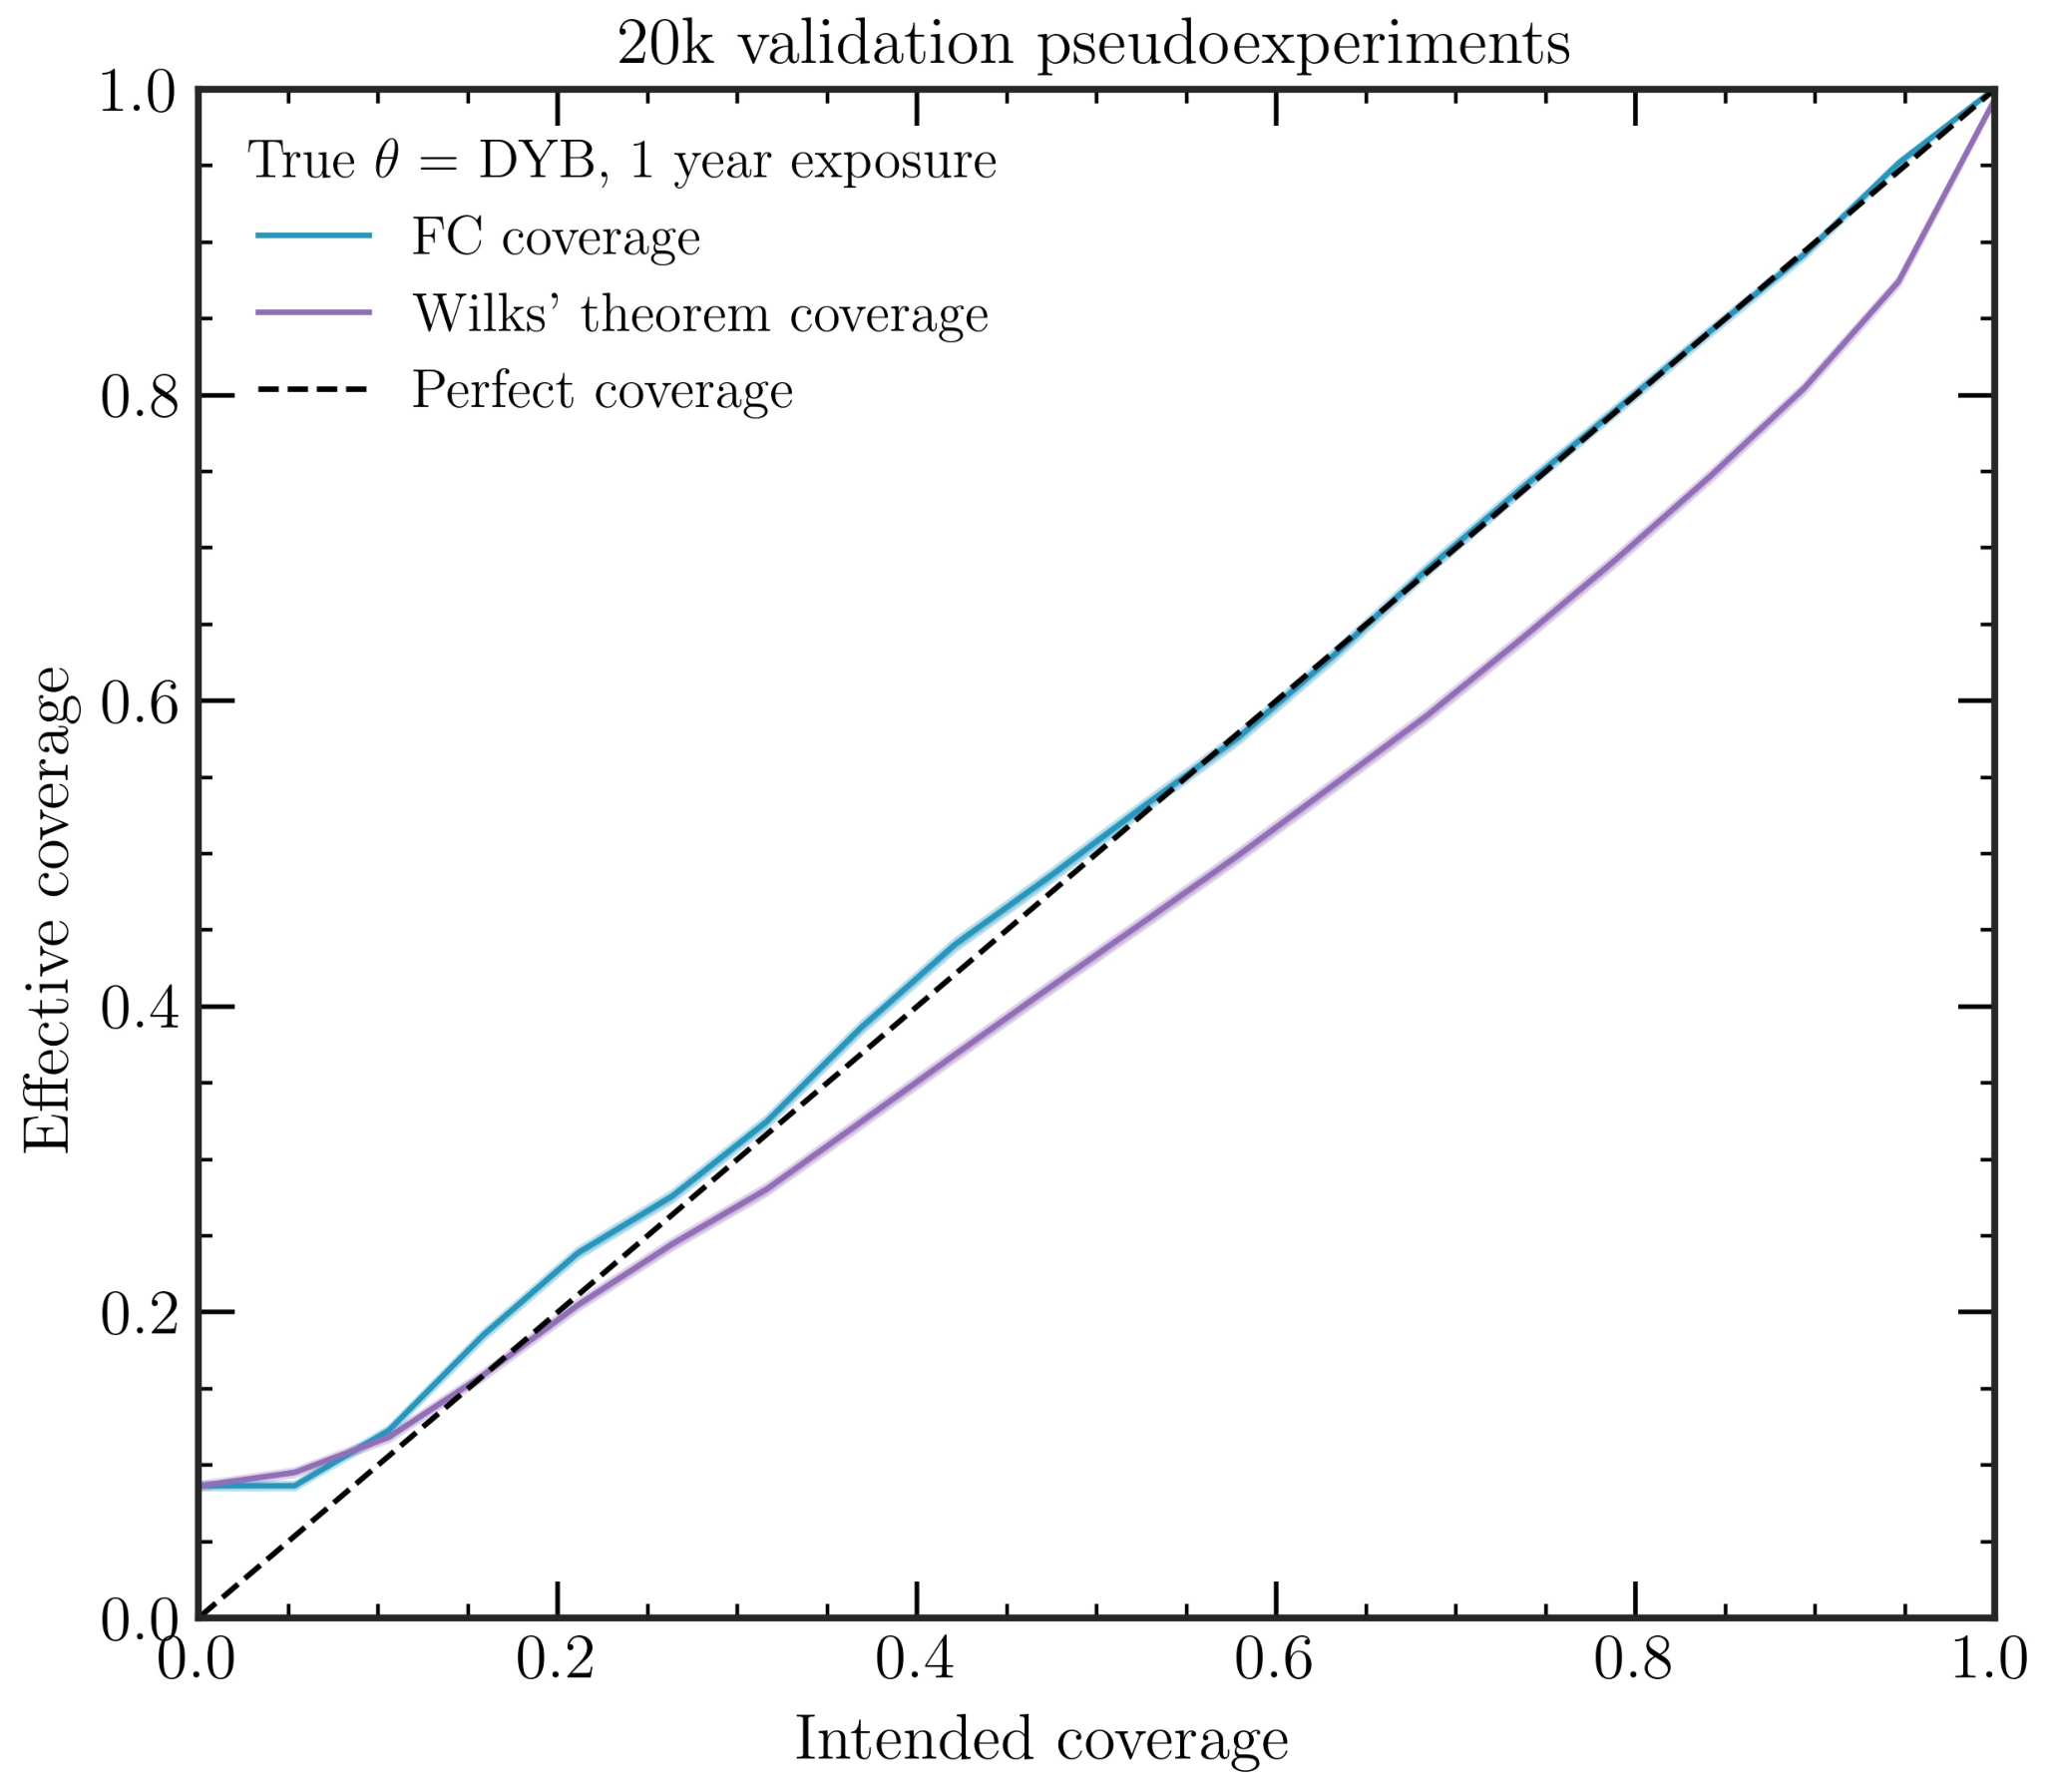
\includegraphics[width=\linewidth]{figs/Section2/vanessa_FC_1y_val_dyb.png}
    \caption{$\theta_0 = \text{DYB}$}
    \label{fig:FC_validation_DYB_1y}
  \end{subfigure}
\hfill
  \begin{subfigure}[t]{0.32\textwidth}
    \centering
    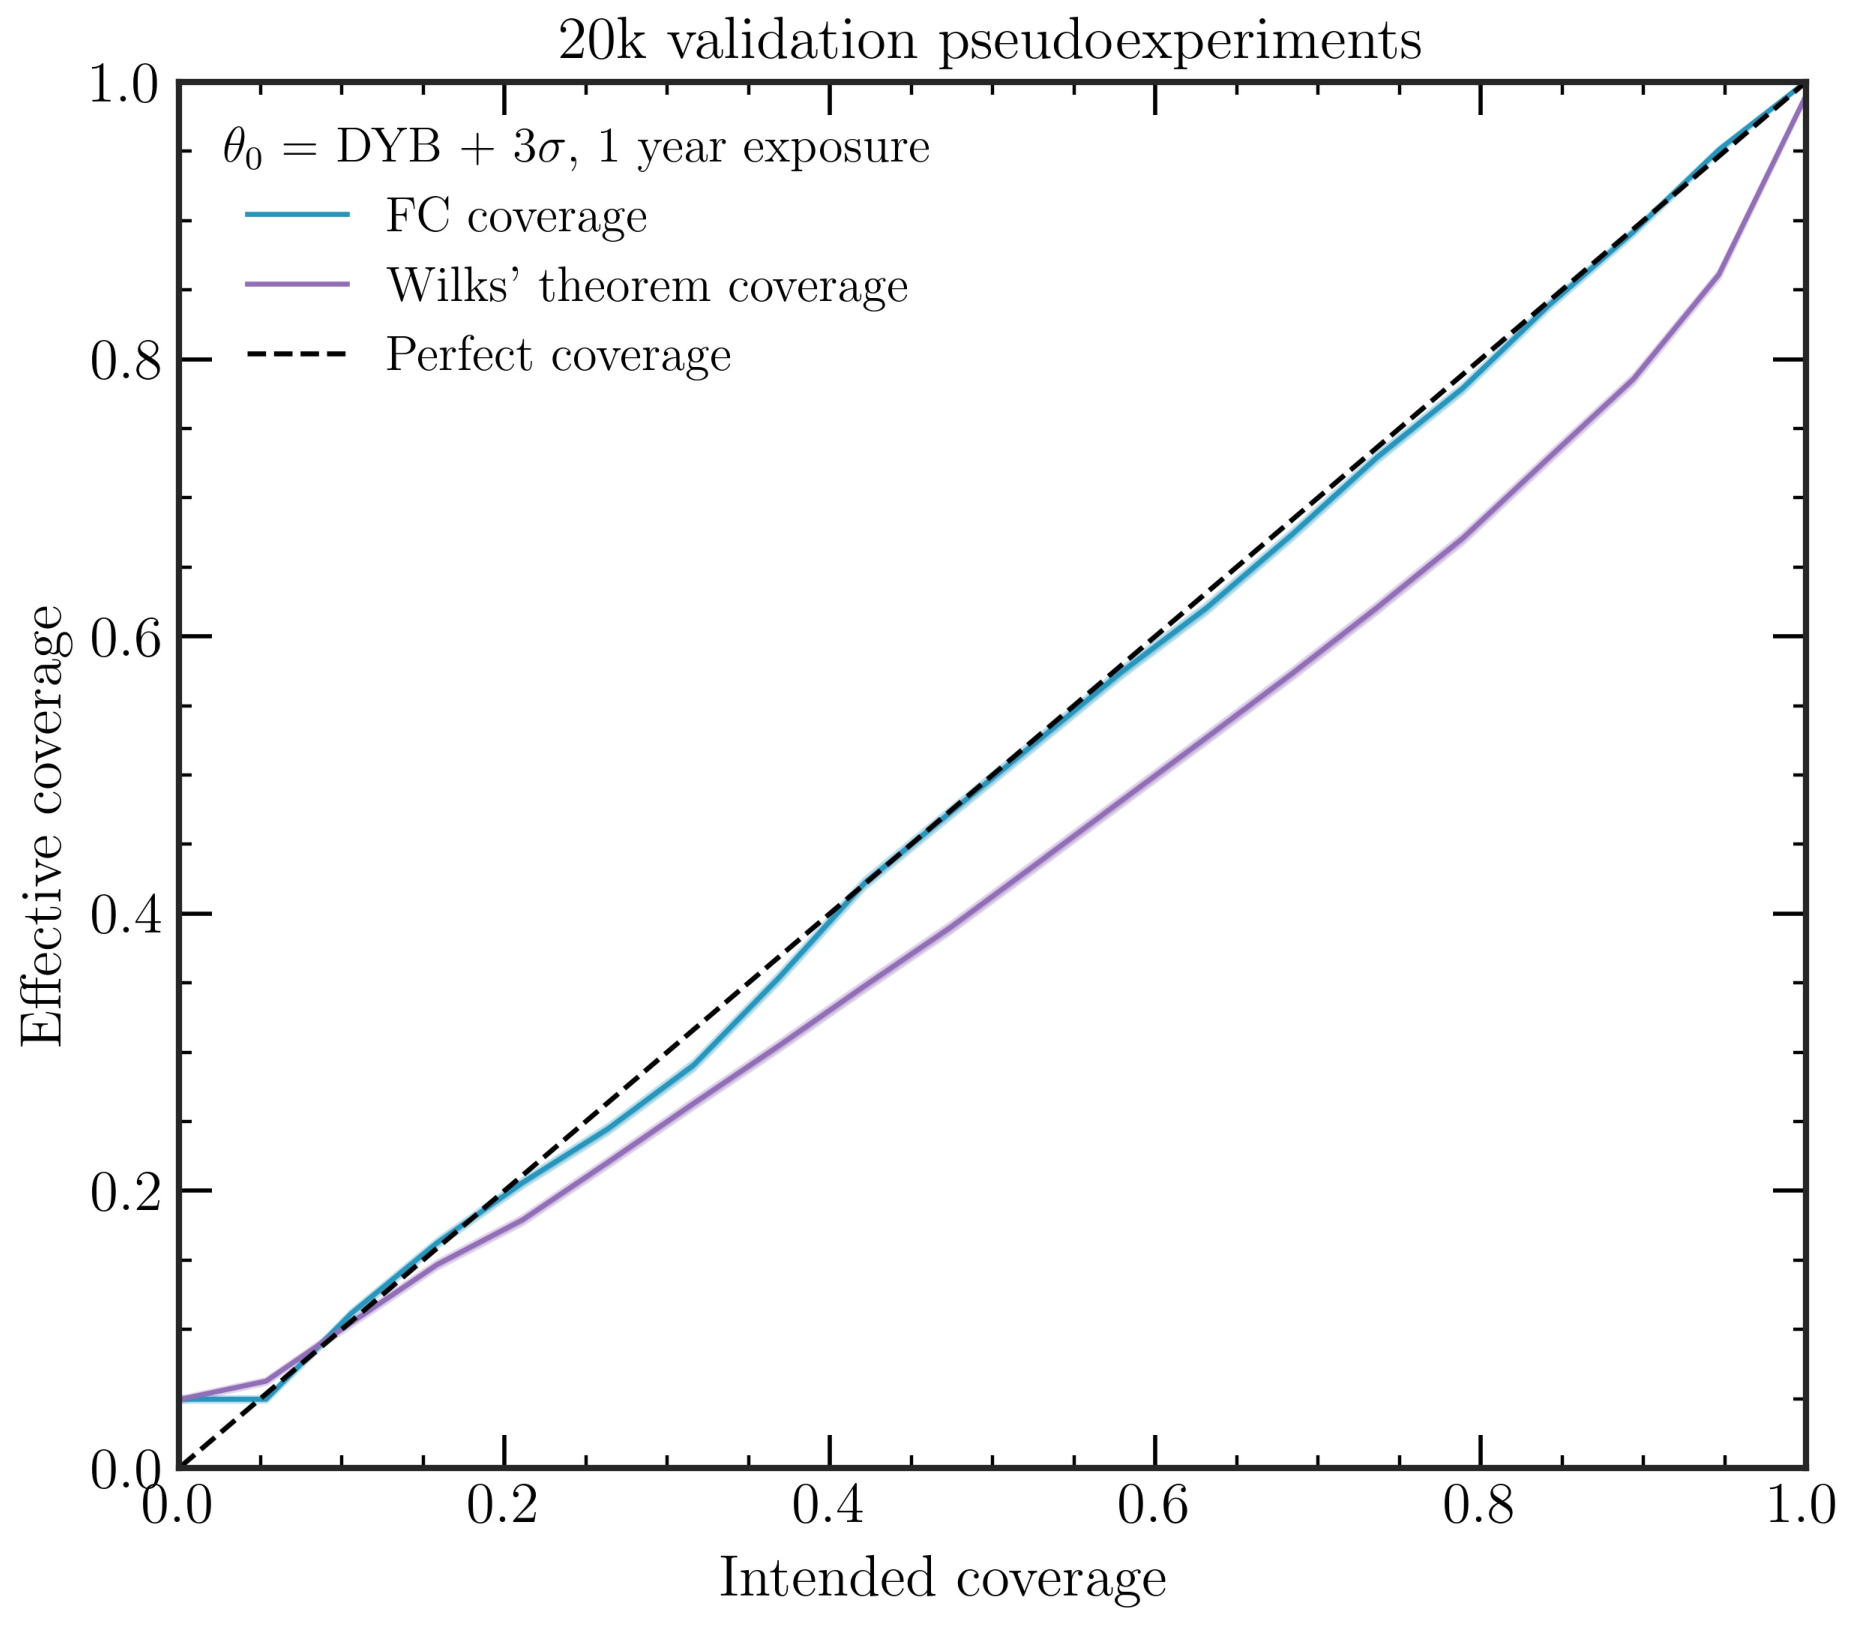
\includegraphics[width=\linewidth]{figs/Section2/vanessa_FC_1y_val_dybp3.png}
    \caption{$\theta_0 = \text{DYB} + 3\sigma$}
    \label{fig:FC_validation_DYBp3s_1y}
  \end{subfigure}
  \caption{Coverage validation across different true values of $\theta_0 = \Delta m_{31}^2$ at 1-year exposure using 20,000 validation pseudoexperiments. }
  \label{fig:FC_validation_1y}
\end{figure}

 \autoref{fig:FC_profile_1year} illustrates the $\Delta \chi^2$ profile of two example validation toys at 1-year exposure. \autoref{fig:FC_profile_1year_single} shows a conventional case where the $\Delta\chi^2$ profile exhibits a relatively smooth, parabolic-like shape near the true value, resulting in a single connected 68.27\% confidence interval (gray shaded region). In contrast, \autoref{fig:FC_profile_1year_double} shows a more complex scenario with multiple disjoint 68.27\% confidence intervals. 


\begin{figure}[ht]
  \centering
  \begin{subfigure}[t]{0.47\textwidth}
    \centering
    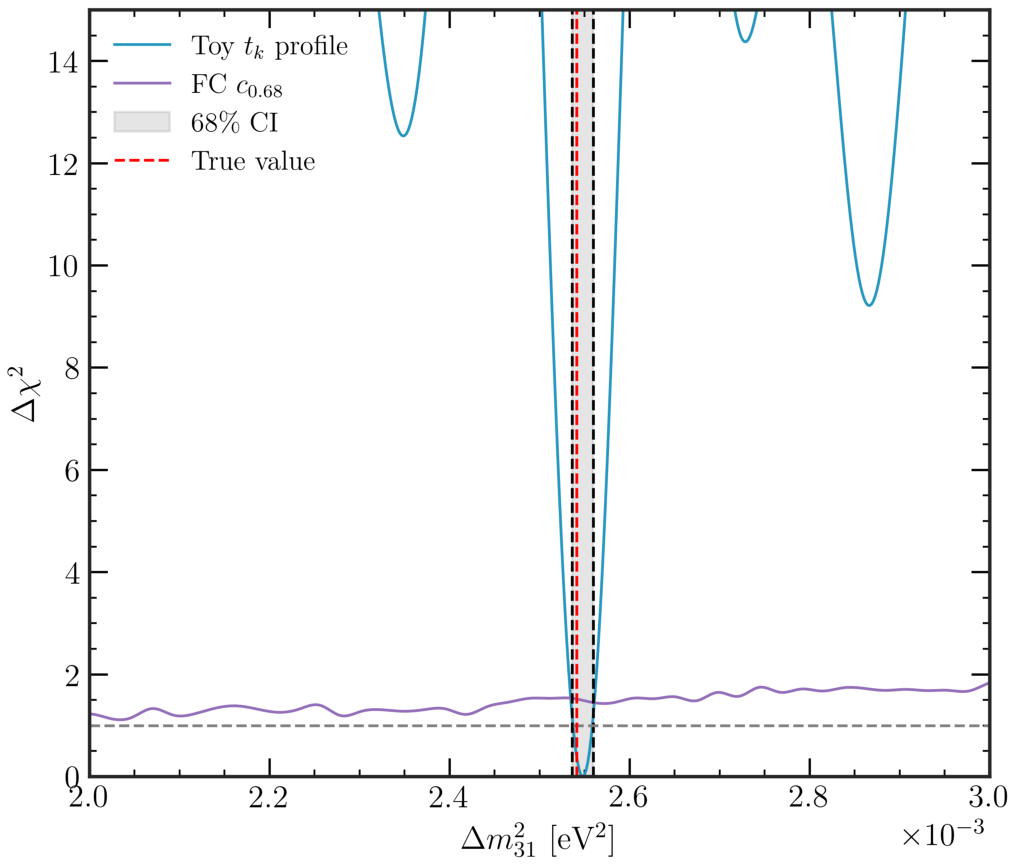
\includegraphics[width=\linewidth]{figs/Section2/vanessa_1year_FC_profile_single.pdf}
    \caption{Example with a single connected 68.27\% confidence interval.}
    \label{fig:FC_profile_1year_single}
  \end{subfigure}
  \hfill
  \begin{subfigure}[t]{0.47\textwidth}
    \centering
    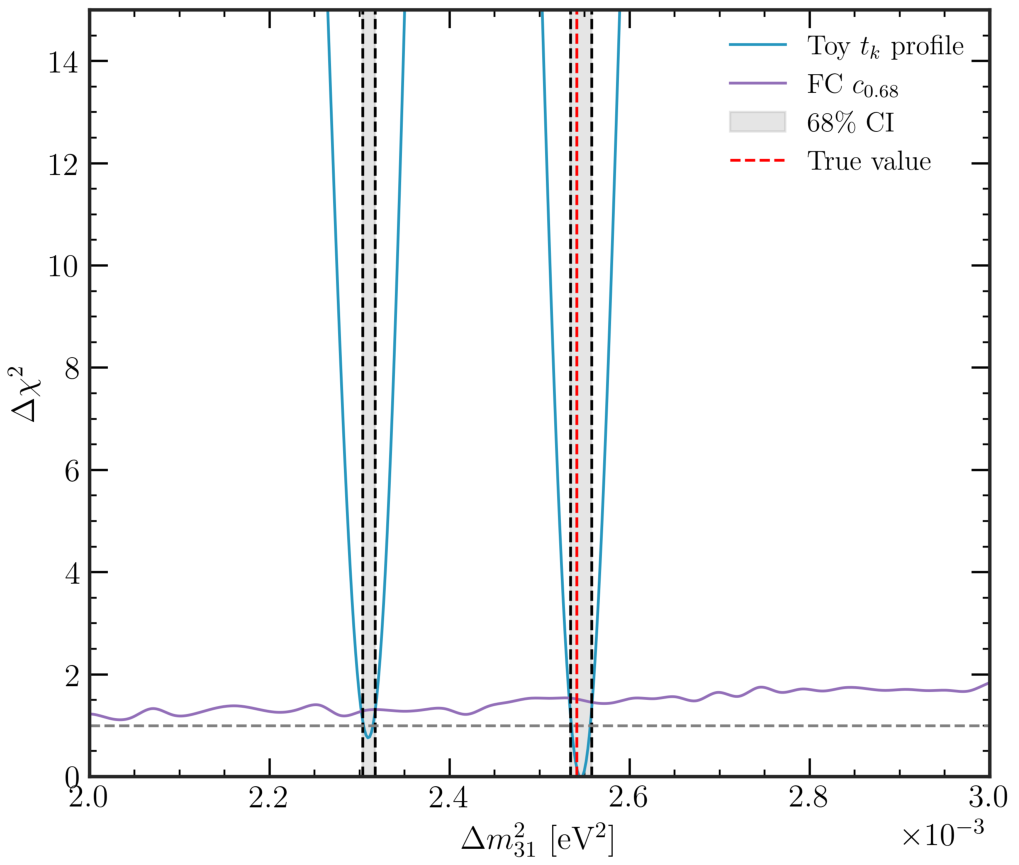
\includegraphics[width=\linewidth]{figs/Section2/vanessa_1year_FC_profile_double.pdf}
    \caption{Example with multiple disjoint 68.27\% confidence intervals.}
    \label{fig:FC_profile_1year_double}
  \end{subfigure}
  \caption{$\Delta \chi^2$ profile for validation pseudoexperiments at 1-year exposure showing different confidence interval topologies. The true value $\theta_0$ is indicated by the red dashed line. The purple line represents the empirical critical values obtained with FC, to be compared with the tabulated value predicted by Wilks' theorem (black dashed line)}
  \label{fig:FC_profile_1year}
\end{figure}

To better understand the degeneracy seen in the confidence intervals during validation, we take a closer look at how often multiple disjoint intervals occur and what their typical structure is. \autoref{fig:FC_degeneracy_1y} shows the distribution of the number of intervals found in 20,000 pseudoexperiments, assuming a 1-year exposure and a true value of $\theta_0 = \text{DYB}$. At the 68.27\% confidence level, i.e., $1\sigma$ level, about 87\% of the pseudoexperiments result in a single interval. In around 10\% of cases, the confidence interval splits into two disjoint regions, and in less than 3\% of cases, more than two intervals are found. The degeneracy becomes more pronounced at higher confidence levels. For 95.45\% intervals, nearly half of the pseudoexperiments produce multiple intervals and at 99.73\%, most pseudoexperiments show multiple disjoint regions. It is worth noting that these results are based on a 1-year exposure. While the occurrence of multiple intervals is rare at the $1\sigma$ level, it becomes much more frequent at $2\sigma$ and $3\sigma$, which should be kept in mind when considering whether to show higher-confidence regions.

\begin{figure}[ht]
  \centering
  \begin{subfigure}[t]{0.32\textwidth}
    \centering
    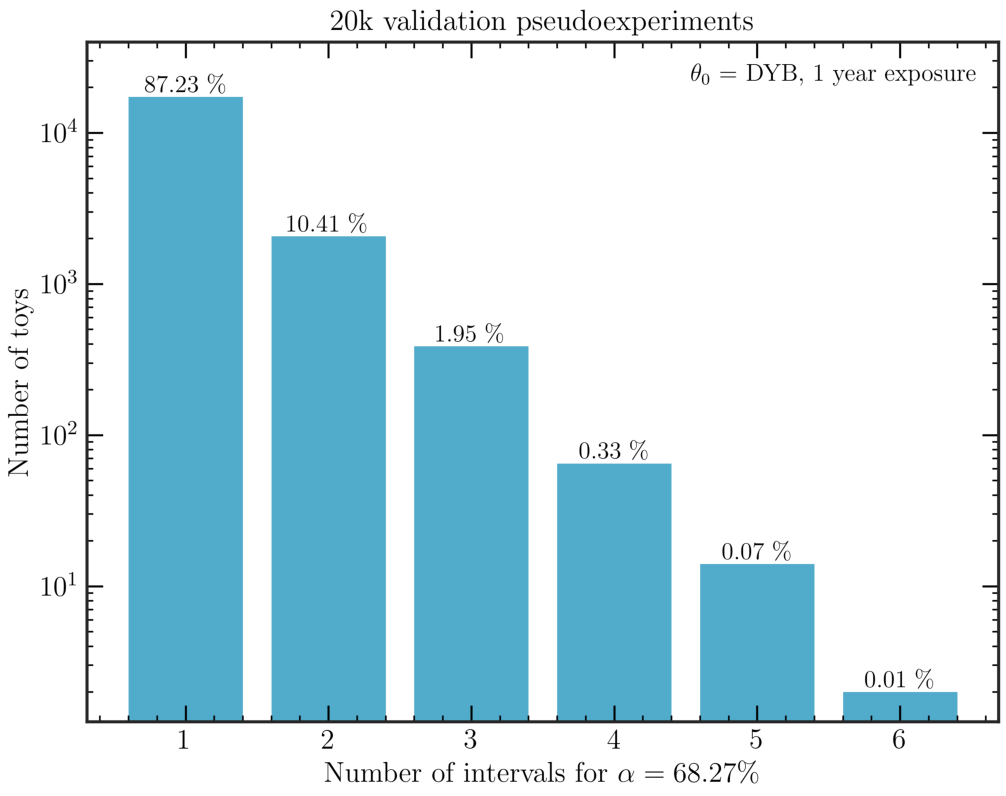
\includegraphics[width=\linewidth]{figs/Section2/vanessa_FC_degeneracy_1y_68.pdf}
    \caption{68.27\% confidence level, $1\sigma$.}
    \label{fig:FC_DYB_1y_deg_68}
  \end{subfigure}
  \hfill
  \begin{subfigure}[t]{0.32\textwidth}
    \centering
    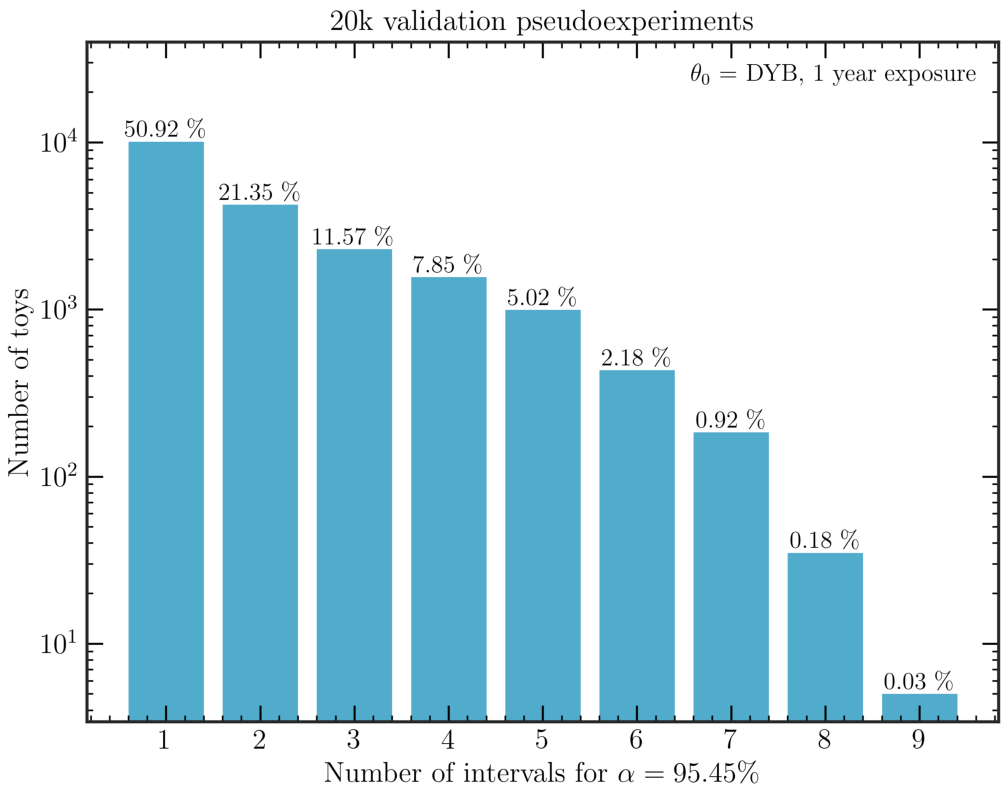
\includegraphics[width=\linewidth]{figs/Section2/vanessa_FC_degeneracy_1y_95.pdf}
    \caption{95.45\% confidence level, $2\sigma$.}
    \label{fig:FC_DYB_1y_deg_95}
  \end{subfigure}
\hfill
  \begin{subfigure}[t]{0.32\textwidth}
    \centering
    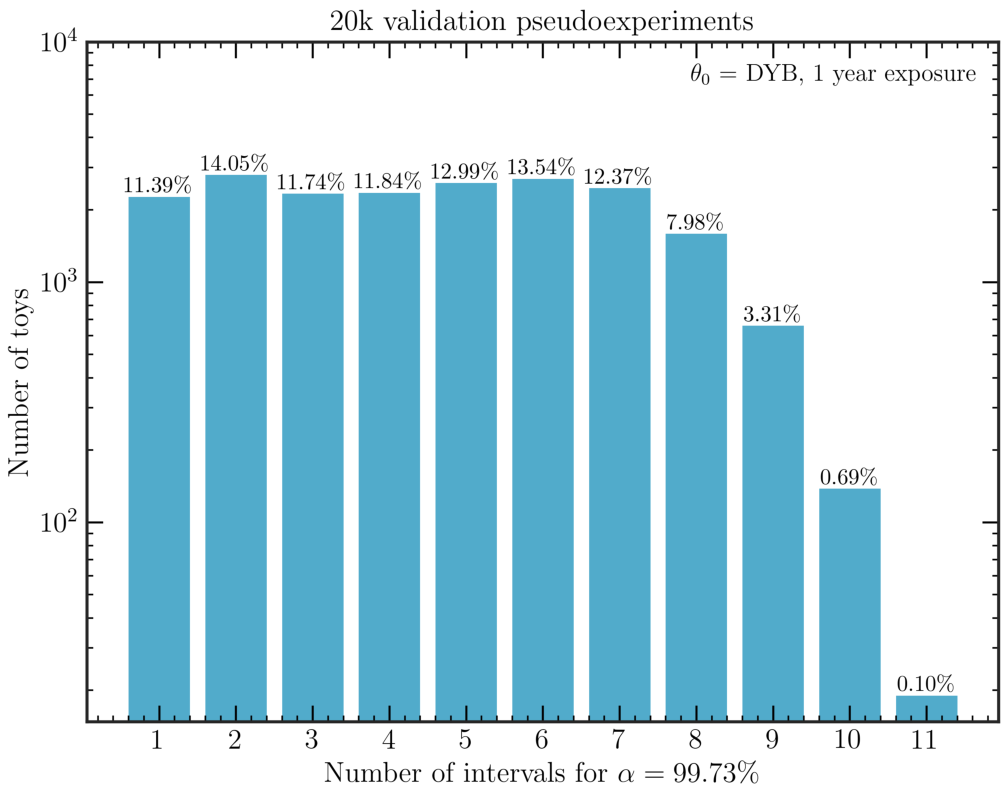
\includegraphics[width=\linewidth]{figs/Section2/vanessa_FC_degeneracy_1y_99.pdf}
    \caption{99.73\% confidence level, $3\sigma$.}
    \label{fig:FC_DYB_1y_deg_99}
  \end{subfigure}
  \caption{Distribution of the number of confidence intervals from 20,000 validation pseudoexperiments at 1-year exposure and with $\theta_0 = \text{DYB}$.}
  \label{fig:FC_degeneracy_1y}
\end{figure}



\subsubsection{$\Delta m^2_{31}$ confidence intervals with FC at low exposure}
To study the behavior of confidence intervals in the low-statistics regime, we carry out a dedicated analysis at 30, 50, and 100 days of exposure, following the same procedure outlined earlier. For each exposure level, we construct parameter grids spanning the physically relevant range of $\Delta m_{31}^2$, generate 5000 pseudoexperiments at each grid point, and determine empirical critical values using the Feldman-Cousins ordering principle.
\autoref{fig:FC_empirical_dist_v} and \autoref{fig:FC_empirical_dist_h} present the empirical test statistic distributions obtained by both analyzers at different exposure levels and at a specific test point.  In both cases, the obtained empirical distributions differ from the theoretical 1 dof $\chi^2$, with much higher critical values compared to Wilks' theorem predictions. \autoref{fig:FC_empirical_dist_v} shows the empirical critical values obtained at different exposure levels, with $c_{68\%} \approx 4.2$ at 50 days and $c_{68\%} \approx 2.8$ at 100 days, both significantly higher than the asymptotic expectation of $\Delta \chi^2 = 1$. Complementary results across a broader exposure range are presented in \autoref{fig:FC_empirical_dist_h}, which shows $\Delta \chi^2_{\text{\rm crit}} = c_{68\%} = 7.05$ at 30 days, 5.63 at 50 days, 4.34 at 100 days, and 1.49 at 1 year.
The discrepancy between the two analyses might be attributed to the difference approaches to nuisance parameter treatment: the implementation of Analyzer 1 uses full profiling over all nuisance parameters for each grid point, while the analysis of Analyzer 2 employs a conditional likelihood approximation where nuisance parameters are fixed to their globally optimized values. The full profiling approach might lead to more conservative critical values since it accounts for the additional uncertainty introduced by optimizing nuisance parameters at each test point, whereas the conditional approach reduces this uncertainty by fixing the nuisance parameters. 


\begin{figure}[ht]
  \centering
  \begin{subfigure}[t]{0.47\textwidth}
    \centering
    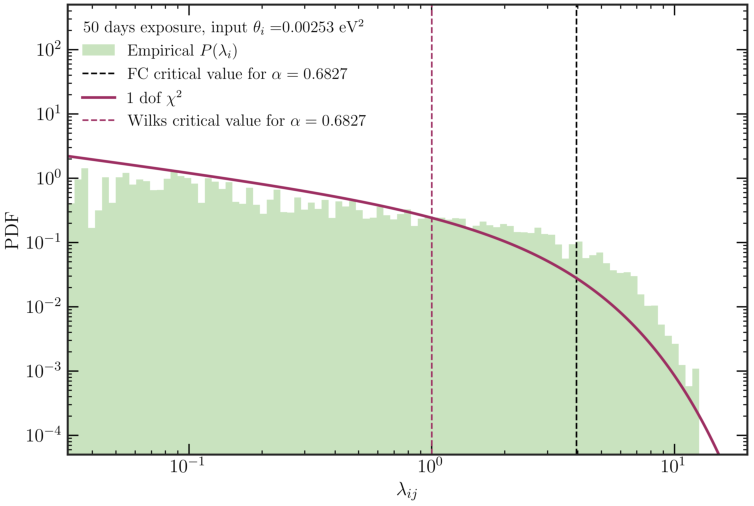
\includegraphics[width=\linewidth]{figs/Section2/vanessa_FC_empirical_dist_50d.pdf}
    \caption{Empirical distribution of test statistic $\lambda_{ij}$ from 5000 toys t 50 days exposure and for $\theta_i = 2.53 \times 10^{-3}$ eV$^2$}
    \label{fig:FC_empirical_dist_50d_v}
  \end{subfigure}
  \hfill
  \begin{subfigure}[t]{0.47\textwidth}
    \centering
    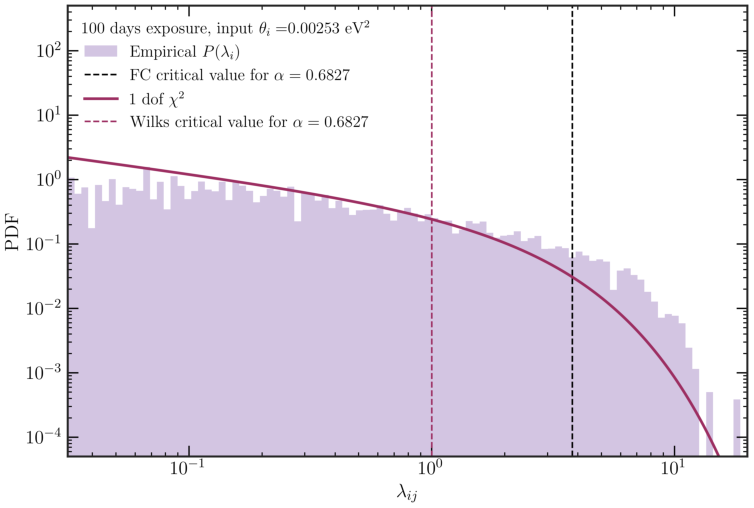
\includegraphics[width=\linewidth]{figs/Section2/vanessa_FC_empirical_dist_100d.pdf}
    \caption{Empirical distribution of test statistic $\lambda_{ij}$ from 5000 toys t 100 days exposure and for $\theta_i = 2.53 \times 10^{-3}$ eV$^2$}
    \label{fig:FC_empirical_dist_100d_v}
  \end{subfigure}
    \caption{Empirical distribution of test statistic $\lambda_{ij}$ from 5000 toys t different exposures.}
  \label{fig:FC_empirical_dist_v}
\end{figure}


\begin{figure}[H]
  \centering 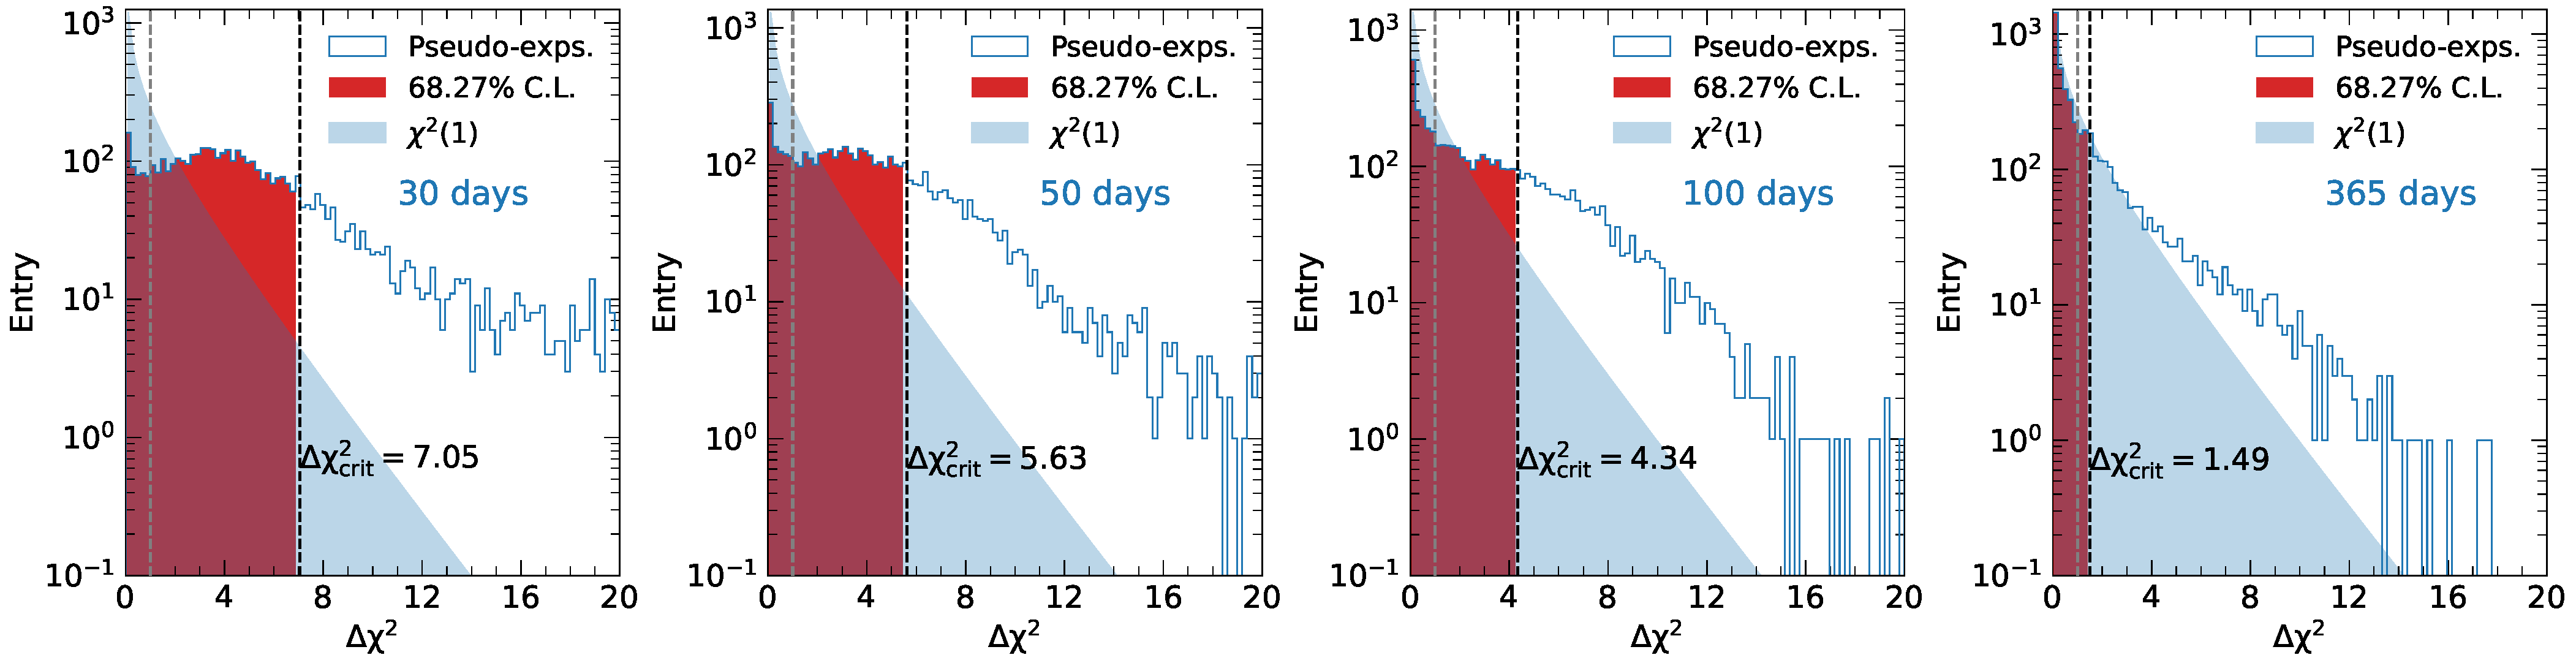
\includegraphics[width=0.96\textwidth]{figs/Section2/han_juno_only_hist_deltachi2_2.5413_2dpull_logV_correct_subplot.pdf}
  \caption{Empirical distribution of test statistic $\Delta\chi^2$ from 5000 toys, assuming a true value of $\Delta m^2_{31}=2.5413\times10^{-3}$ $\rm{eV^2}$ for 4 data-taking durations.} 
  \label{fig:FC_empirical_dist_h}
\end{figure}

20,000 pseudoexperiments with known true value $\theta_0= \text{DYB}$ are generated at 50 and 100 days exposure to check the coverage properties and study the degeneracy of confidence intervals, following the same procedure outlined in the previous paragraph.
\autoref{fig:FC_coverage_low_exposure} compares the coverage of the FC method (blue curves) and Wilks’ theorem (purple curves) for $\theta_0 = \text{DYB}$, for 50 days  (\autoref{fig:FC_coverage_50d}) and 100 days (\autoref{fig:FC_coverage_100d}) exposure.  
The results demonstrate that Wilks' theorem significantly undercovers at low exposure, achieving roughly 20\% effective coverage instead of the intended 68\%. This points to a failure of the asymptotic approximation, since the actual coverage turns out to be less than one-third of the nominal confidence level. FC procedure instead provides very accurate coverage. This highlights the importance of using FC in order to maintain proper statistical inference at low exposures.

\begin{figure}[H]
  \centering
  \begin{subfigure}[t]{0.47\textwidth}
    \centering
    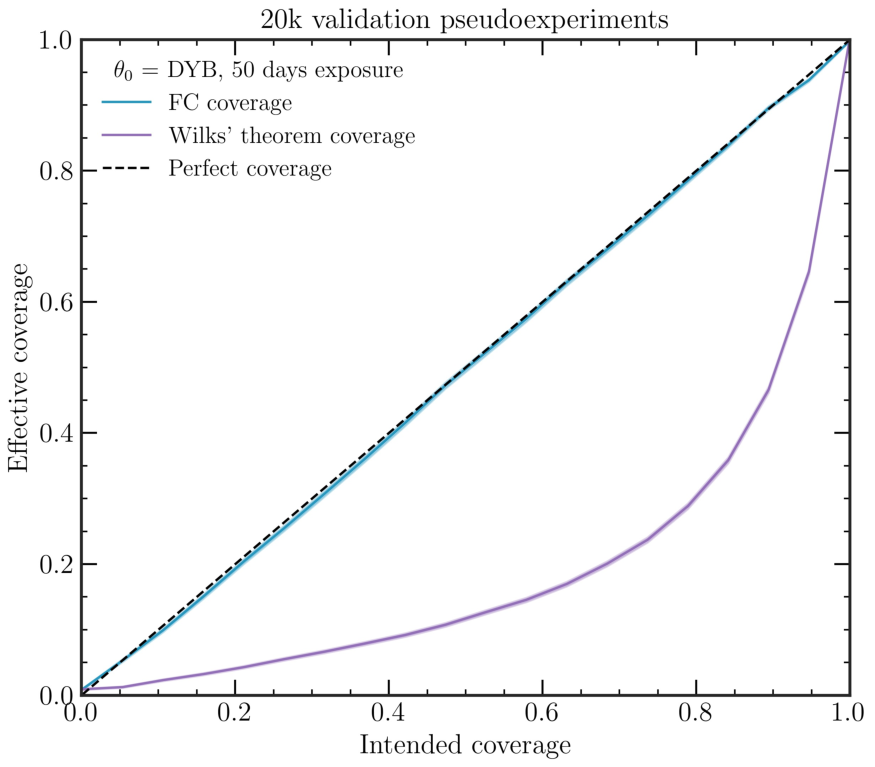
\includegraphics[width=\linewidth]{figs/Section2/vanessa_FC_coverage_50d.pdf}
    \caption{Coverage validation at 50 days exposure}
    \label{fig:FC_coverage_50d}
  \end{subfigure}
  \hfill
  \begin{subfigure}[t]{0.47\textwidth}
    \centering
    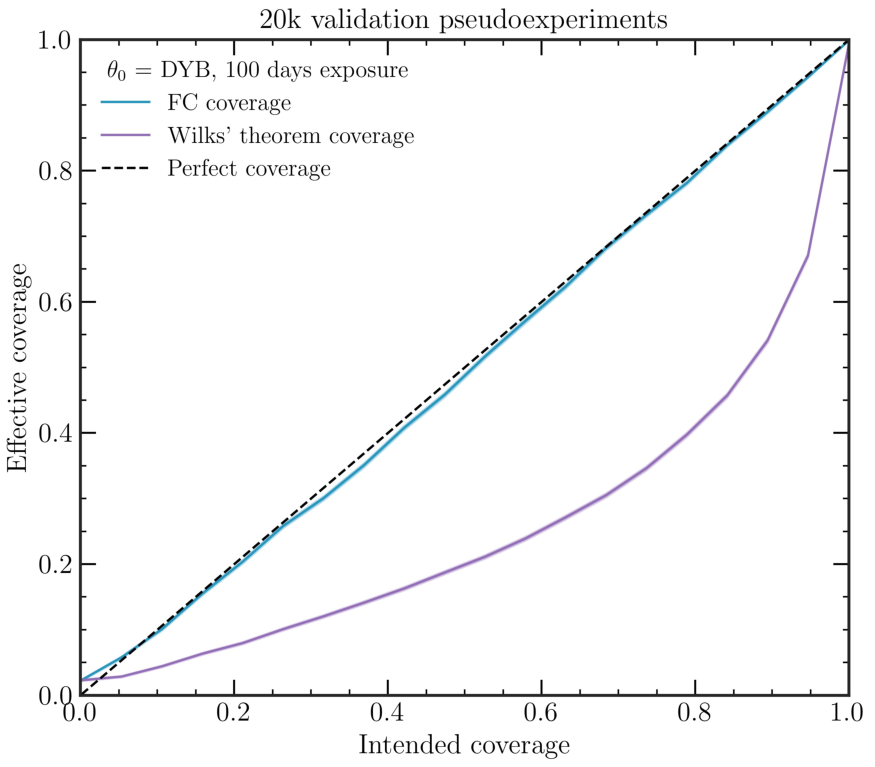
\includegraphics[width=\linewidth]{figs/Section2/vanessa_FC_coverage_100d.pdf}
    \caption{Coverage validation at 100 days exposure}
    \label{fig:FC_coverage_100d}
  \end{subfigure}
  \caption{Coverage validation results at low exposures showing the comparison between FC method (blue) and Wilks' theorem (purple).}
  \label{fig:FC_coverage_low_exposure}
\end{figure}


\begin{figure}[H]
  \centering
  \begin{subfigure}[t]{0.47\textwidth}
    \centering
    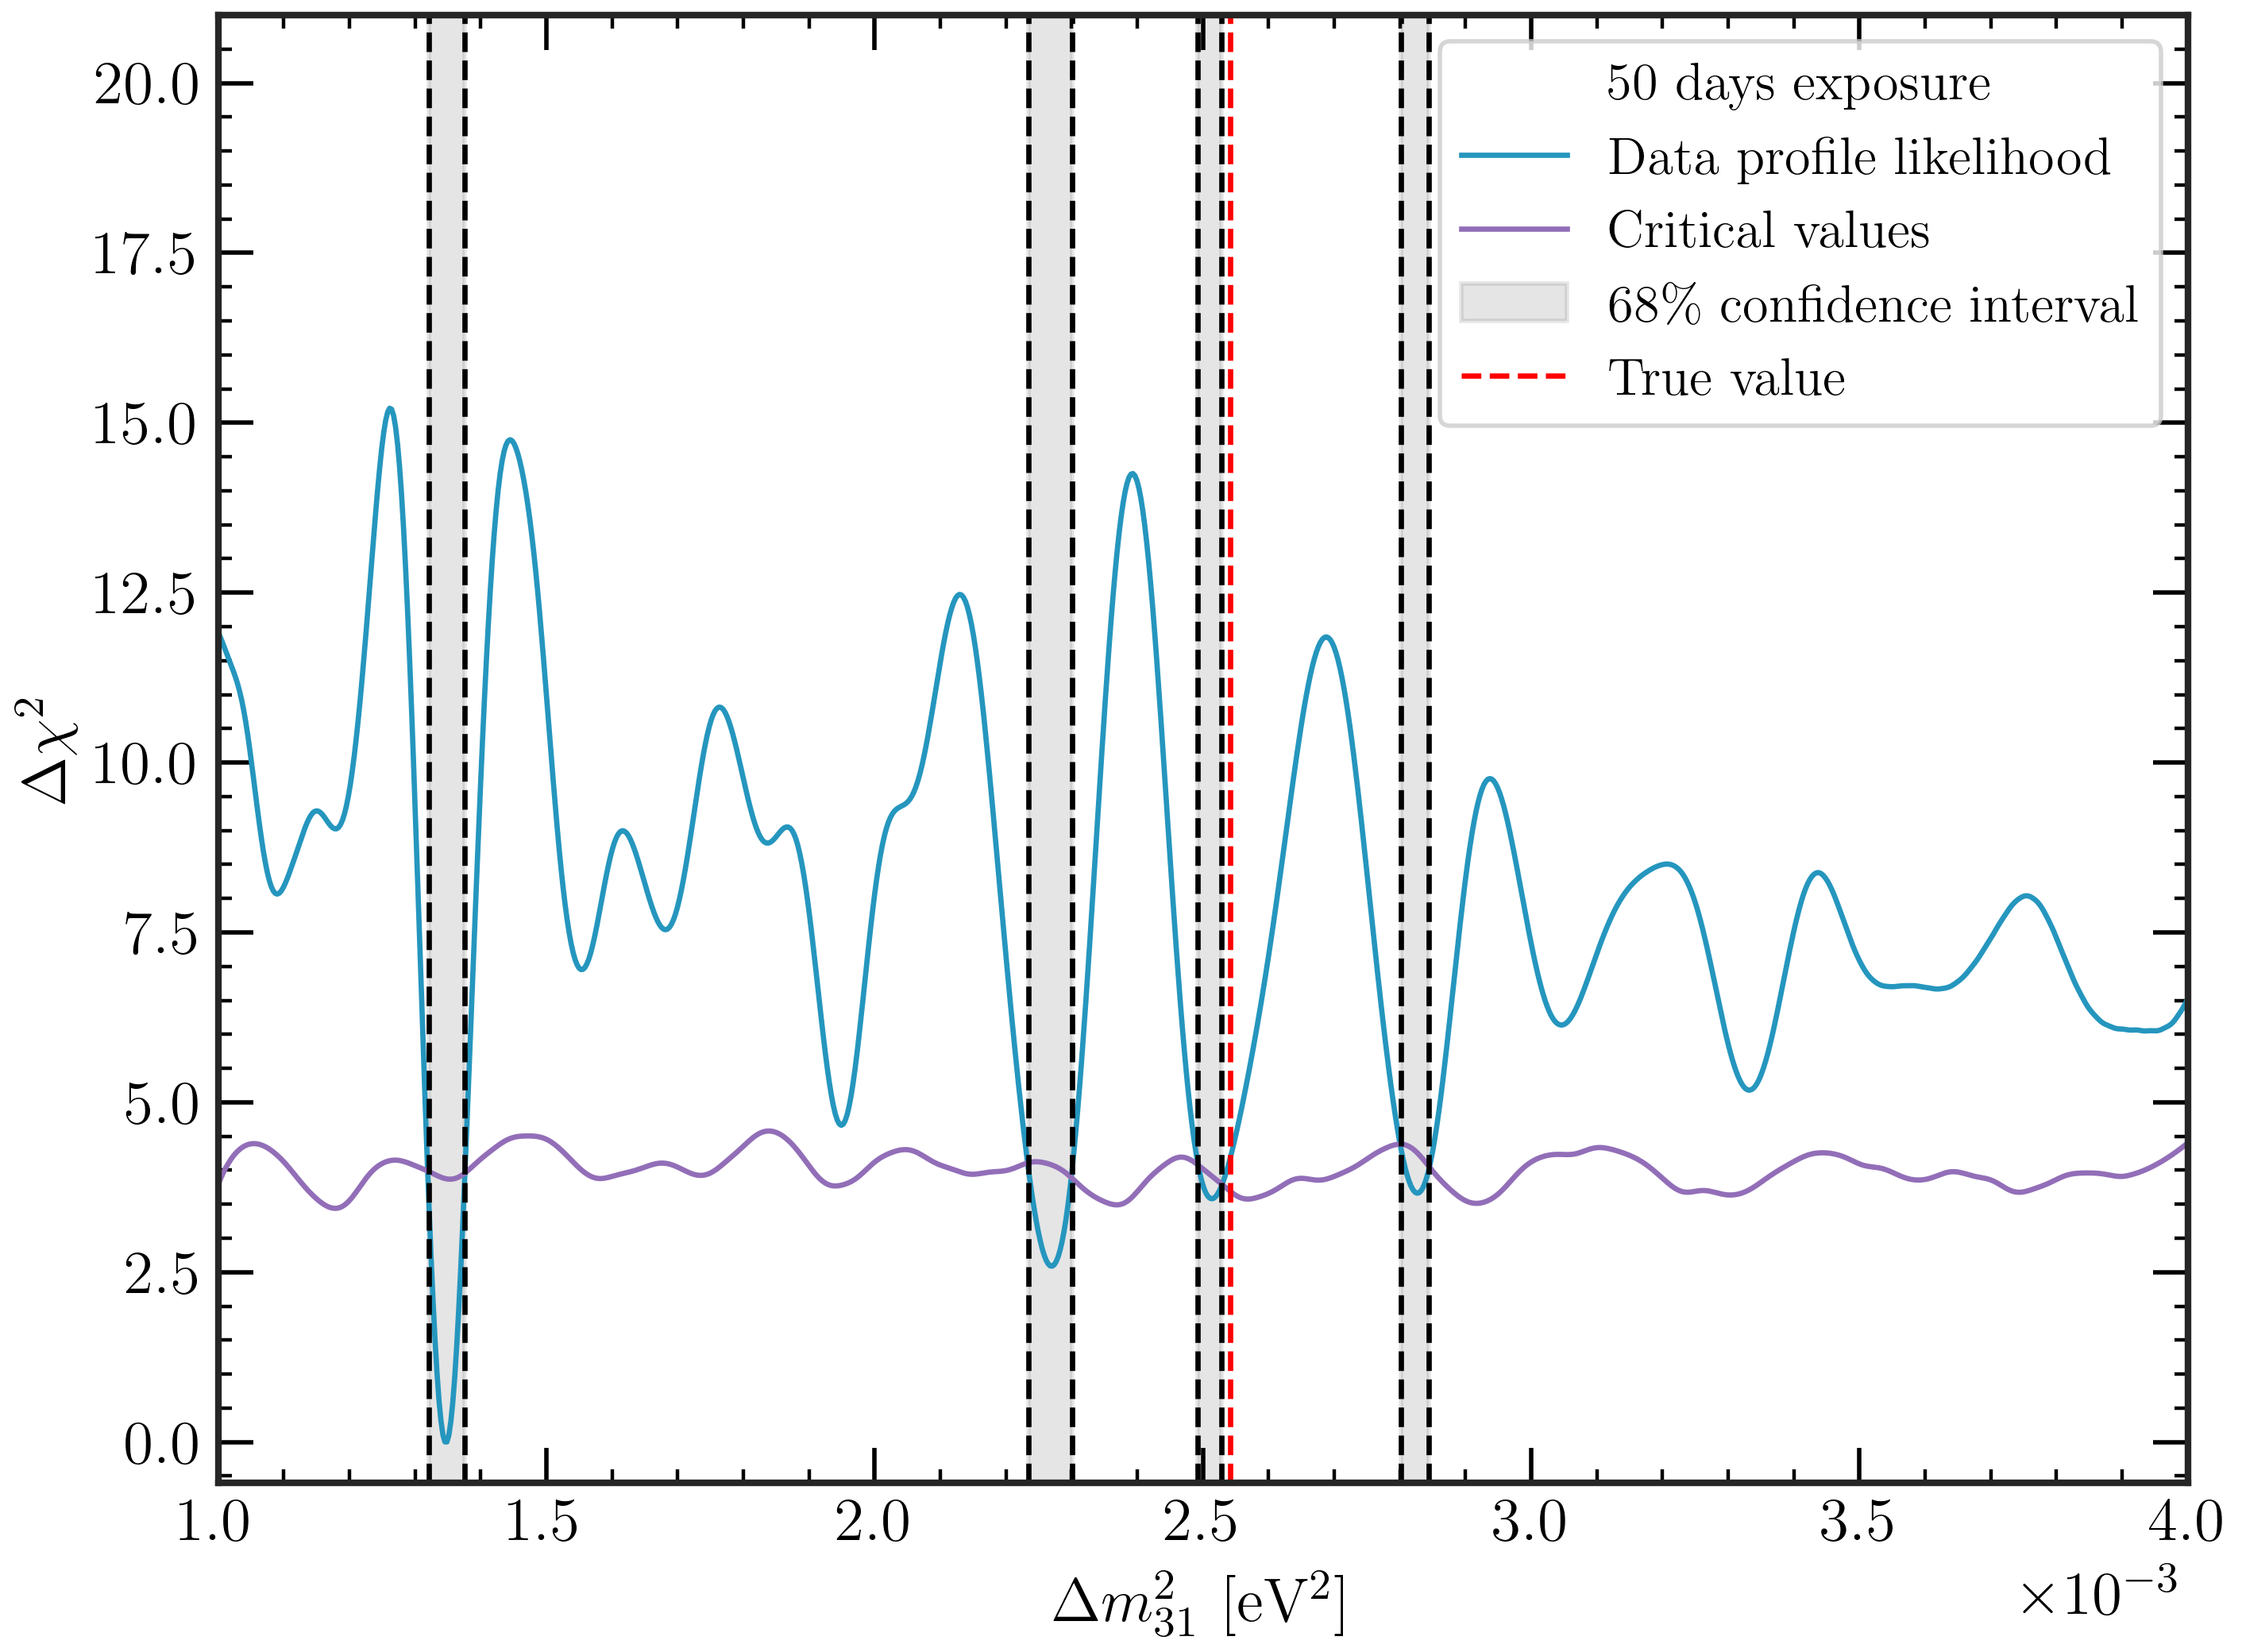
\includegraphics[width=\linewidth]{figs/Section2/FC_profile_toy_196.png}
    \caption{Example of $\Delta\chi^2$ profile and FC critical values at 50 days exposure.}
    \label{fig:FC_profile_50d}
  \end{subfigure}
  \hfill
  \begin{subfigure}[t]{0.47\textwidth}
    \centering
    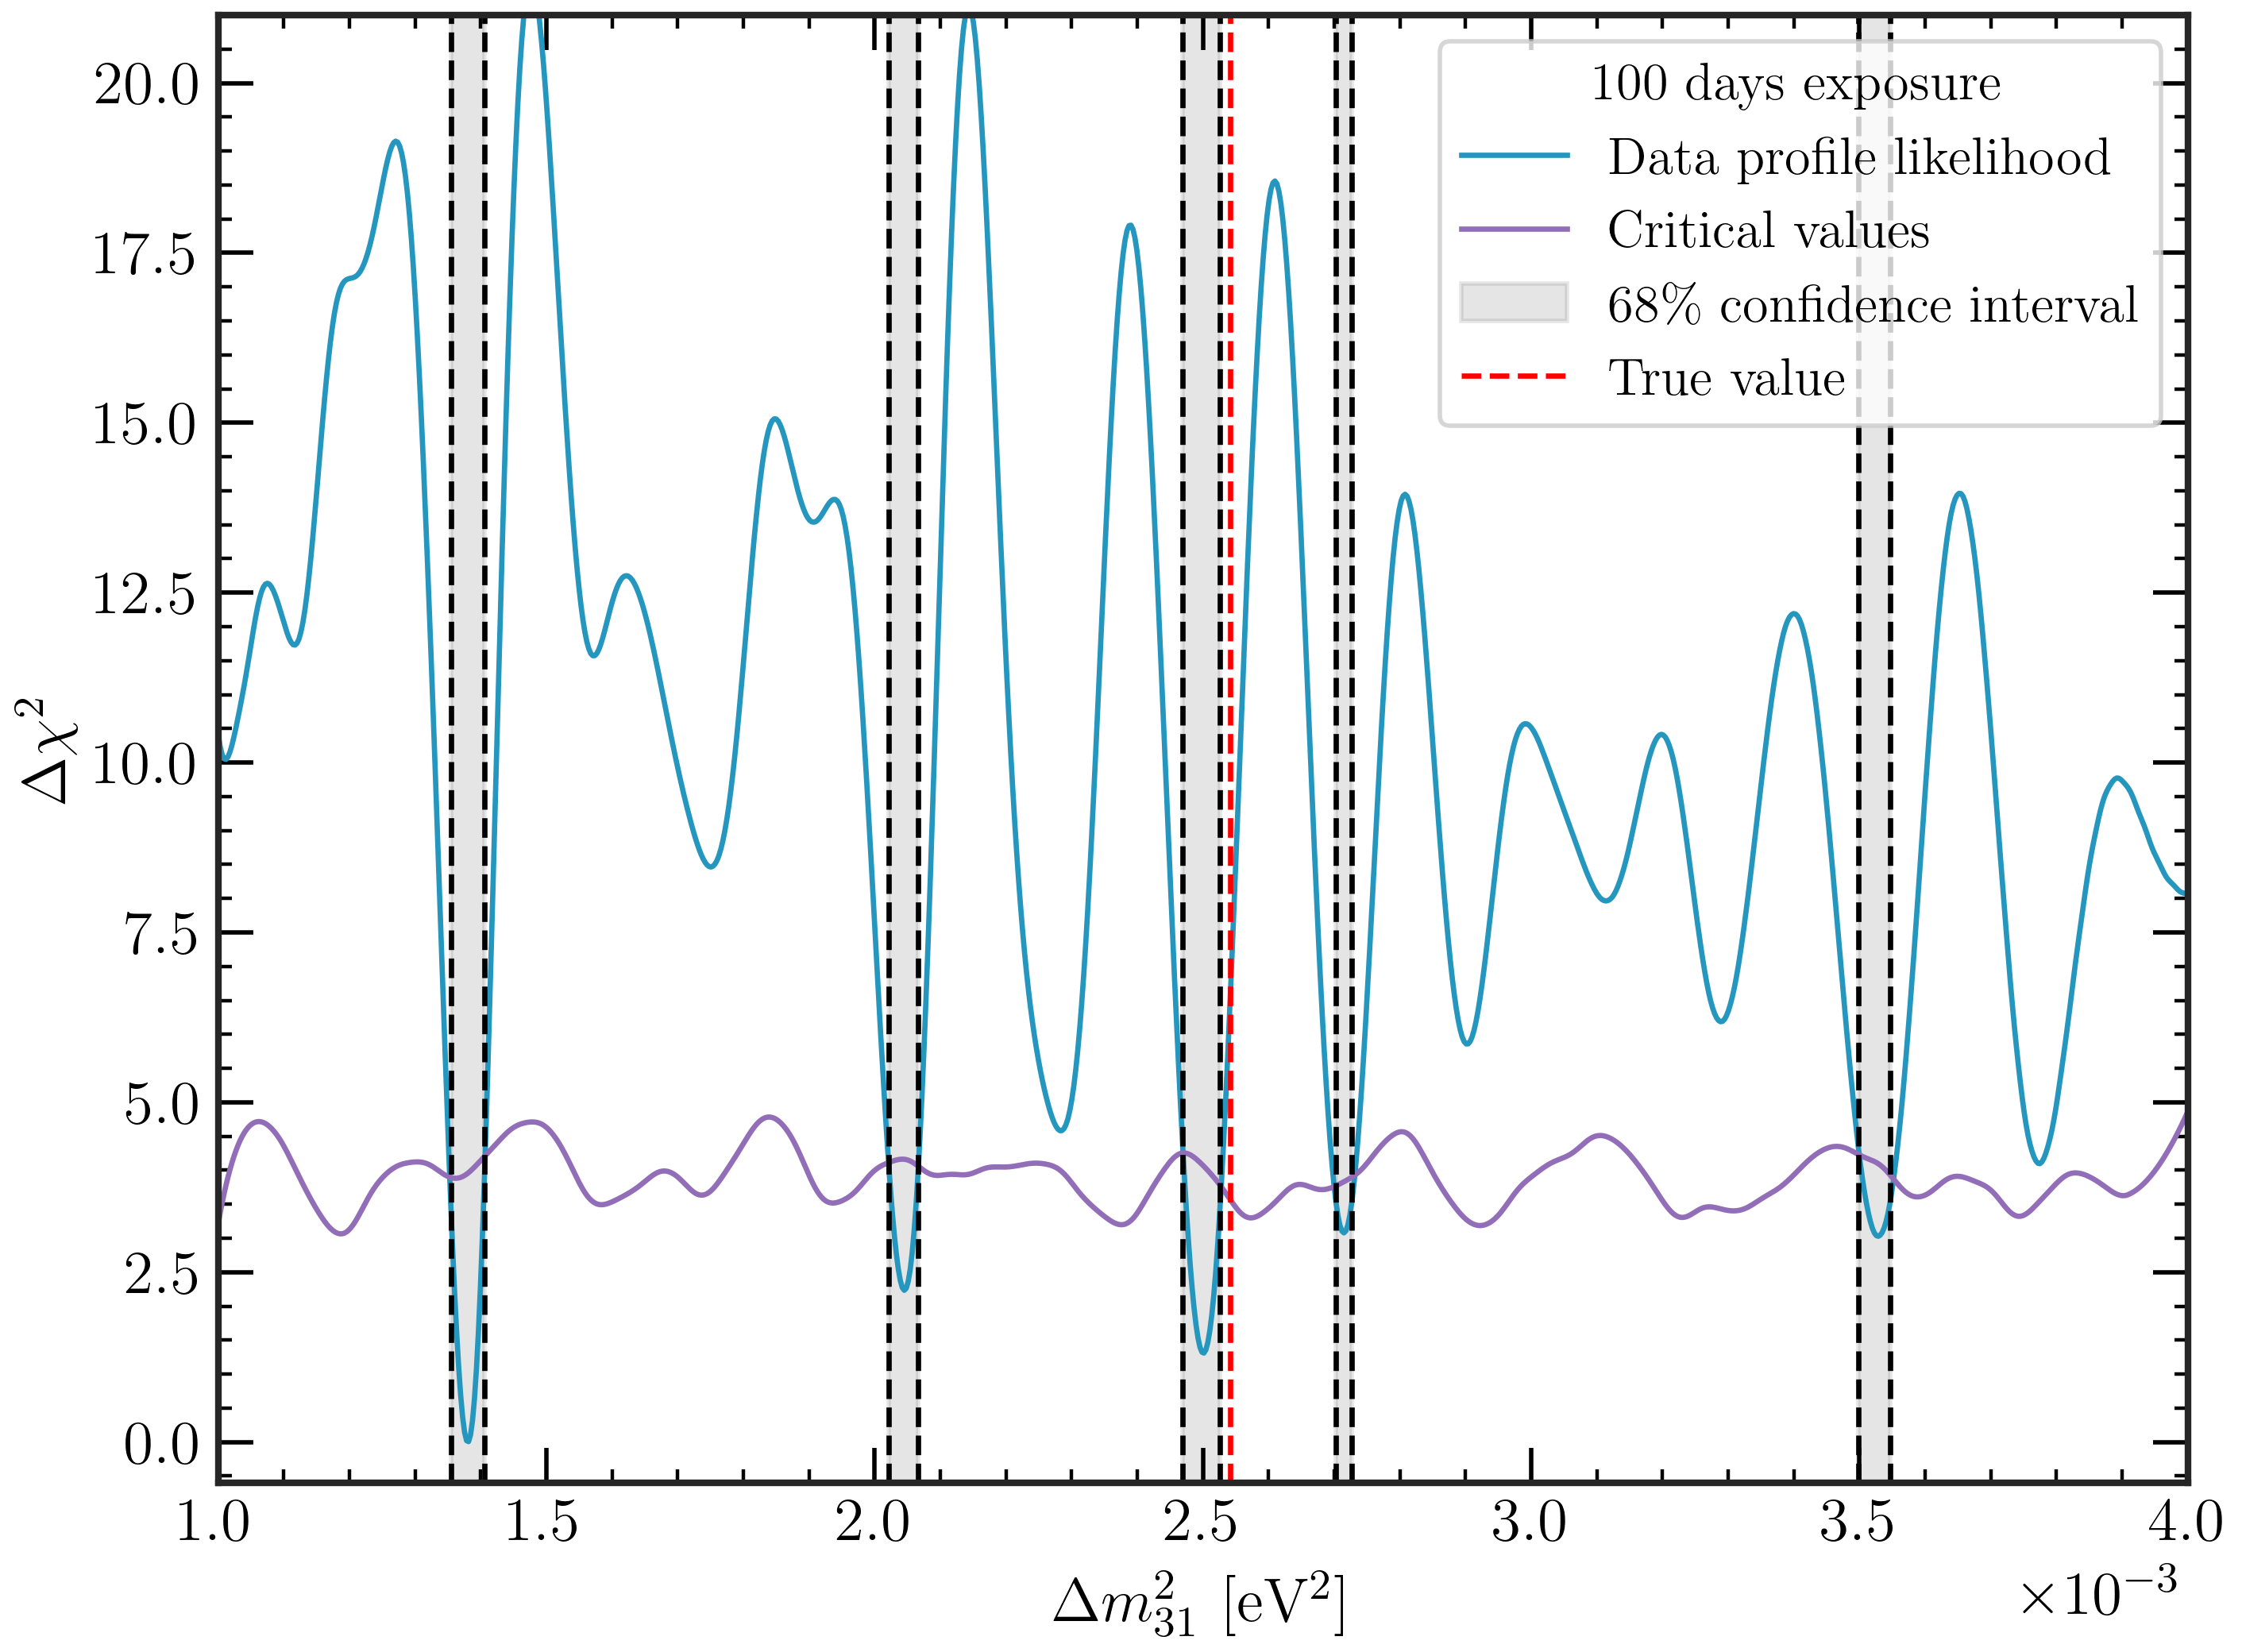
\includegraphics[width=\linewidth]{figs/Section2/FC_profile_toy_123_100d.png}
    \caption{Example of $\Delta\chi^2$ profile and FC critical values at 100 days exposure.}
    \label{fig:FC_profile_100d}
  \end{subfigure}
  \caption{$\Delta\chi^2$ profiles (blue lines), with confidence intervals (gray shaded areas) and critical values (violet lines) for 68.27\% confidence level. Examples for 50 days and 100 days exposure. }
  \label{fig:FC_profiles_50_100}
\end{figure}


\begin{figure} [H]
  \centering 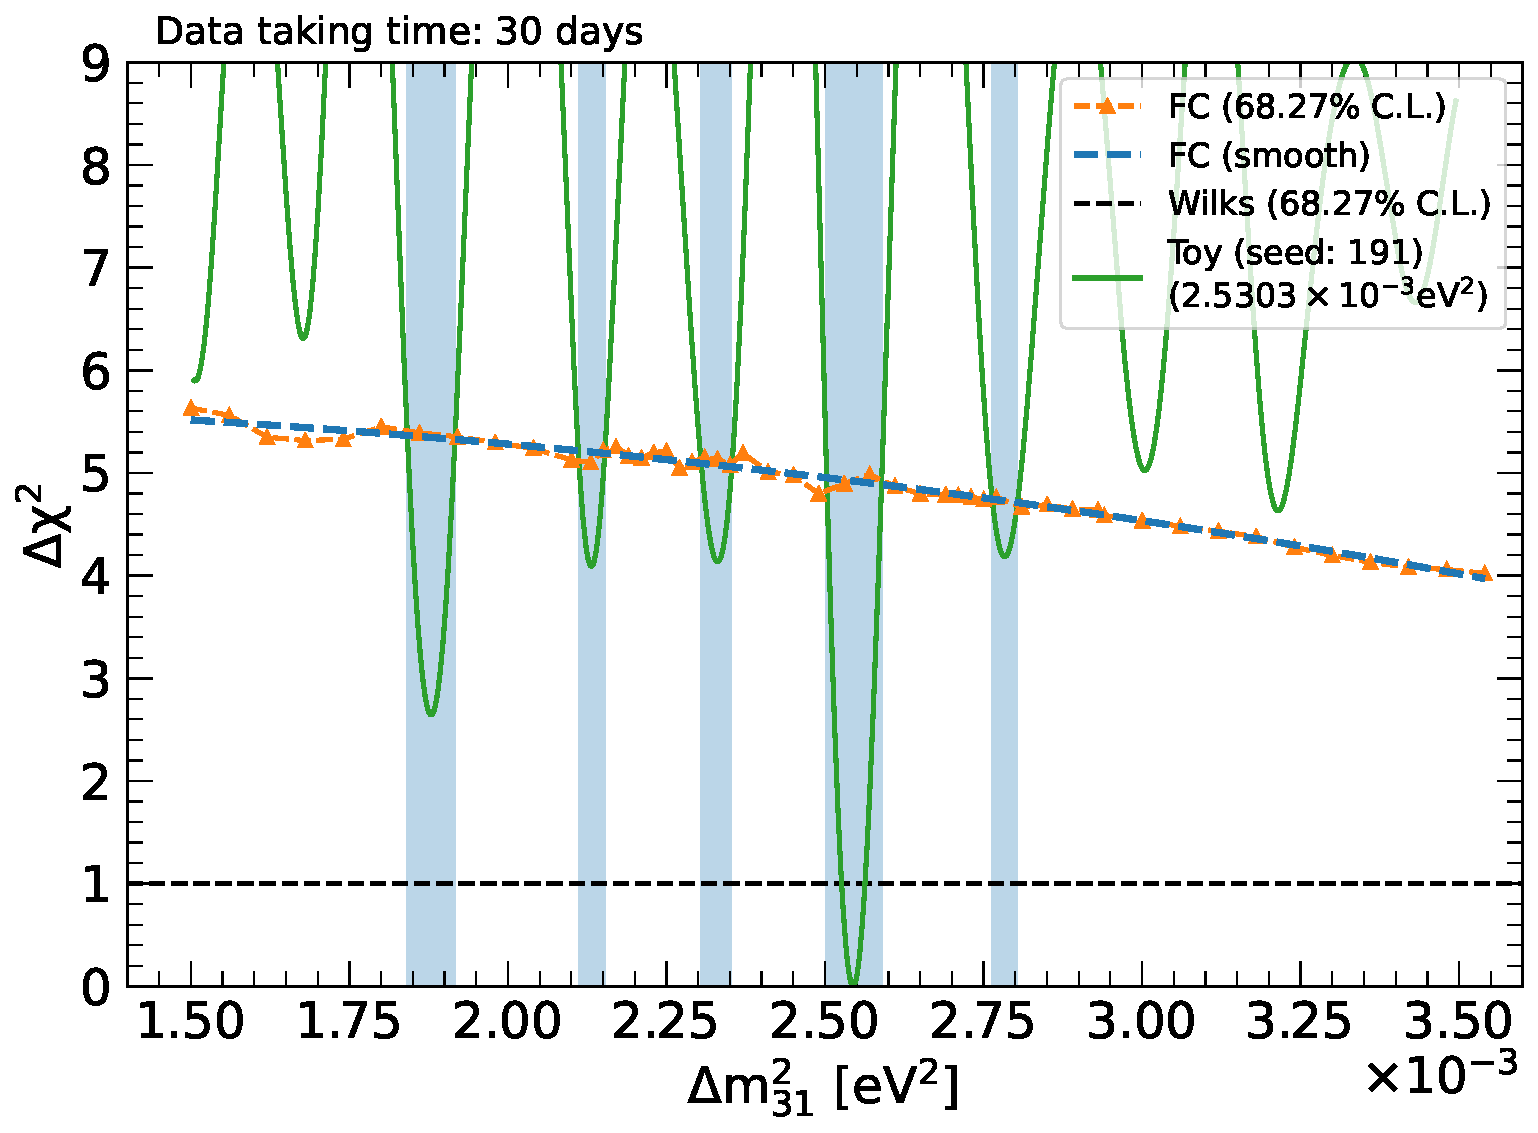
\includegraphics[width=0.8\textwidth]{figs/Section2/han_juno_only_profile_example.pdf}
  \caption{Example of $\Delta\chi^2$ profile (green line) showing confidence intervals (blue spans) and critical values (blue line) for 68.27\% confidence level. Since the critical values are larger than those form Wilks, the probability of having disjointed intervals greatly increases when using FC, i.e, a proper statistical treatment.}
  \label{fig:example_juno_only_profile_30days}
\end{figure}

\begin{figure} [h]
    \centering
    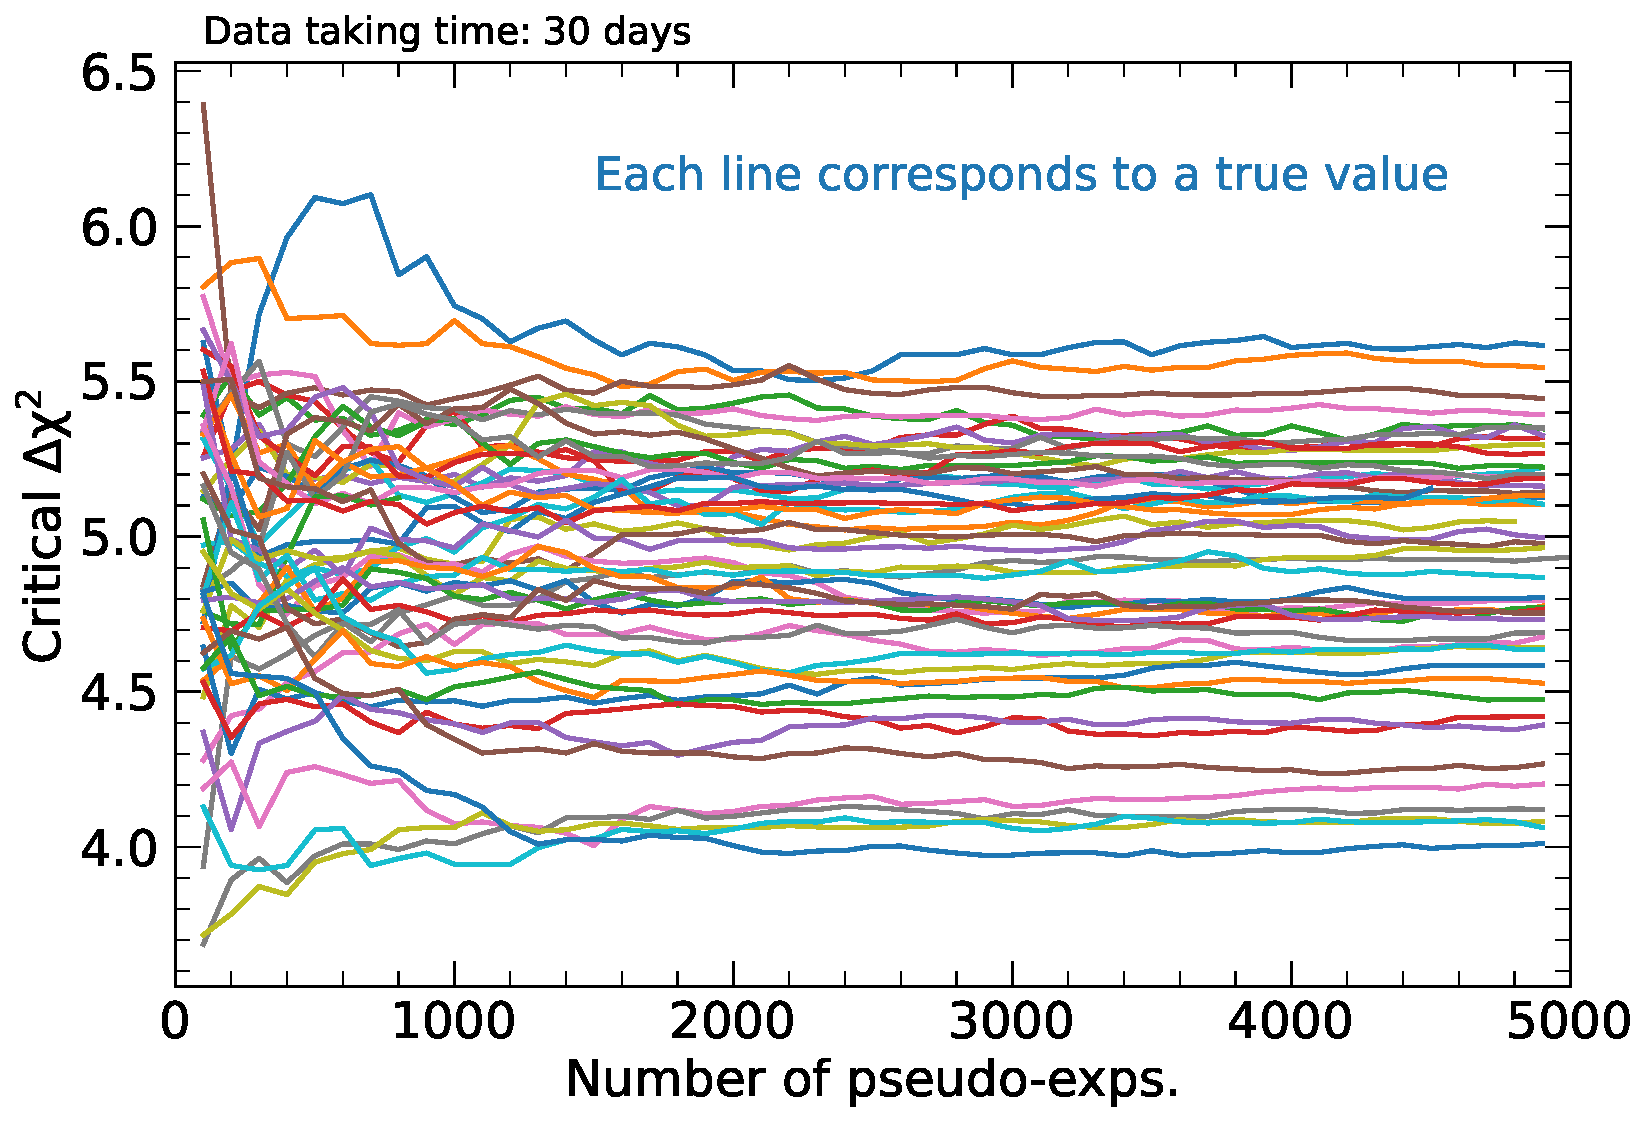
\includegraphics[width=0.8\linewidth]{figs/Section2/han_juno_only_critical_deltachi2_fluctuate_caveat.pdf}
    \caption{Critical value as a function of toy amount}
    \label{fig:crit_val_vs_toy_num}
\end{figure}



\autoref{fig:FC_profiles_50_100} and \autoref{fig:example_juno_only_profile_30days} show examples of $\Delta\chi^2$ profiles and the corresponding critical values for the 68.27\% confidence level at exposures of 100, 50, and 30 days. In all cases, multiple disjoint 68.27\% confidence intervals are observed.
The FC critical values are obtained with empirical distributions assuming different true values. To mitigate the potential impact of statistical fluctuations on critical values, we note from \autoref{fig:crit_val_vs_toy_num} that the critical value fluctuates within about $\pm0.1$ and tends to stabilize as the number of pseudo-experiments increases. 

\autoref{fig:FC_degeneracy_all_68} shows the confidence interval degeneracy for several exposures: 1 year (blue), 100 days (green), and 50 days (violet). Each bar corresponds to a different exposure and the y-axis reports the fraction of toys with a given number of $1\sigma$ confidence intervals. As shown in \autoref{fig:FC_DYB_1y_deg_68}, at 1 year exposure, most cases (roughly $87\%$) have a single interval. These percentage significantly drops at lower exposures. Indeed, at 50 days approximately 97\% of pseudoexperiments result in multiple disjoint confidence intervals.  The fraction of multiple intervals decreases to 87\% at 100 days exposure, but still represents the vast majority of measurements. It is worth noting that, given that the FC critical values are higher than Wilks', we have a higher probability of having disjointed intervals than what is reported in \autoref{sec:2_bad_minima}. 


\begin{figure}[H]
  \centering 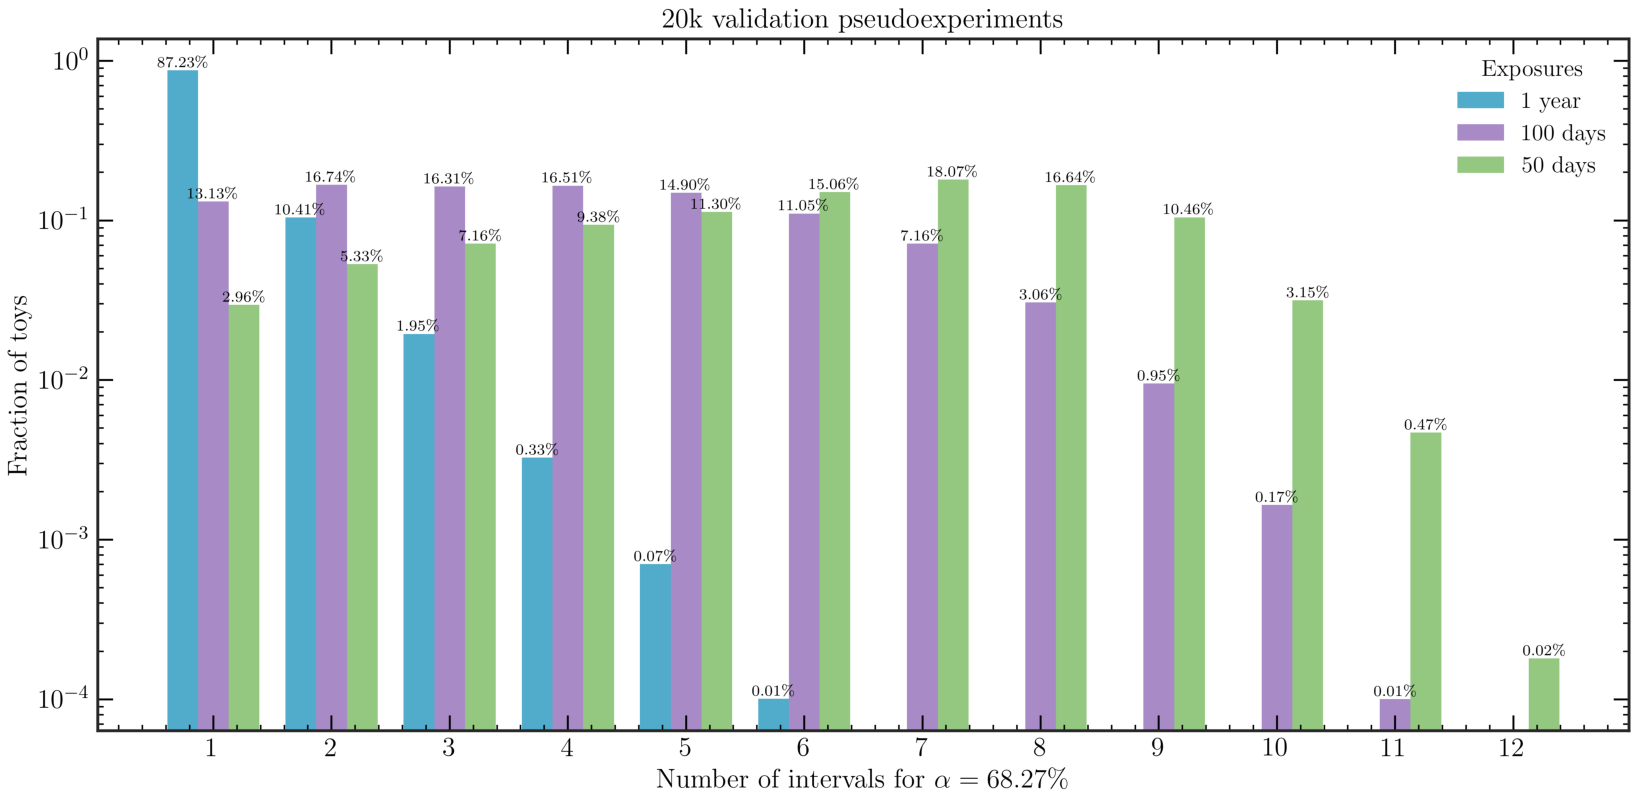
\includegraphics[width=0.9\textwidth]{figs/Section2/vanessa_FC_degeneracy_all_68.pdf}
  \caption{$1\sigma$ confidence interval degeneracy for different exposures: 1 year (blue), 100 days (green), 50 days (violet). }
  \label{fig:FC_degeneracy_all_68}
\end{figure}


\subsubsection{Evolution of critical values with exposure}
\autoref{fig:FC_exposure_h} shows the evolution of the $1\sigma$ confidence level critical value as a function of data-taking time; it shows a gradual transition from the non-asymptotic regime at low exposures to the asymptotic behavior predicted by Wilks' theorem. The critical value approaches the Wilks' theorem prediction of $\Delta\chi^2 = 1$ (black dashed line) but does not reach this value until approximately 500 days of exposure.

\begin{figure}[H]
  \centering 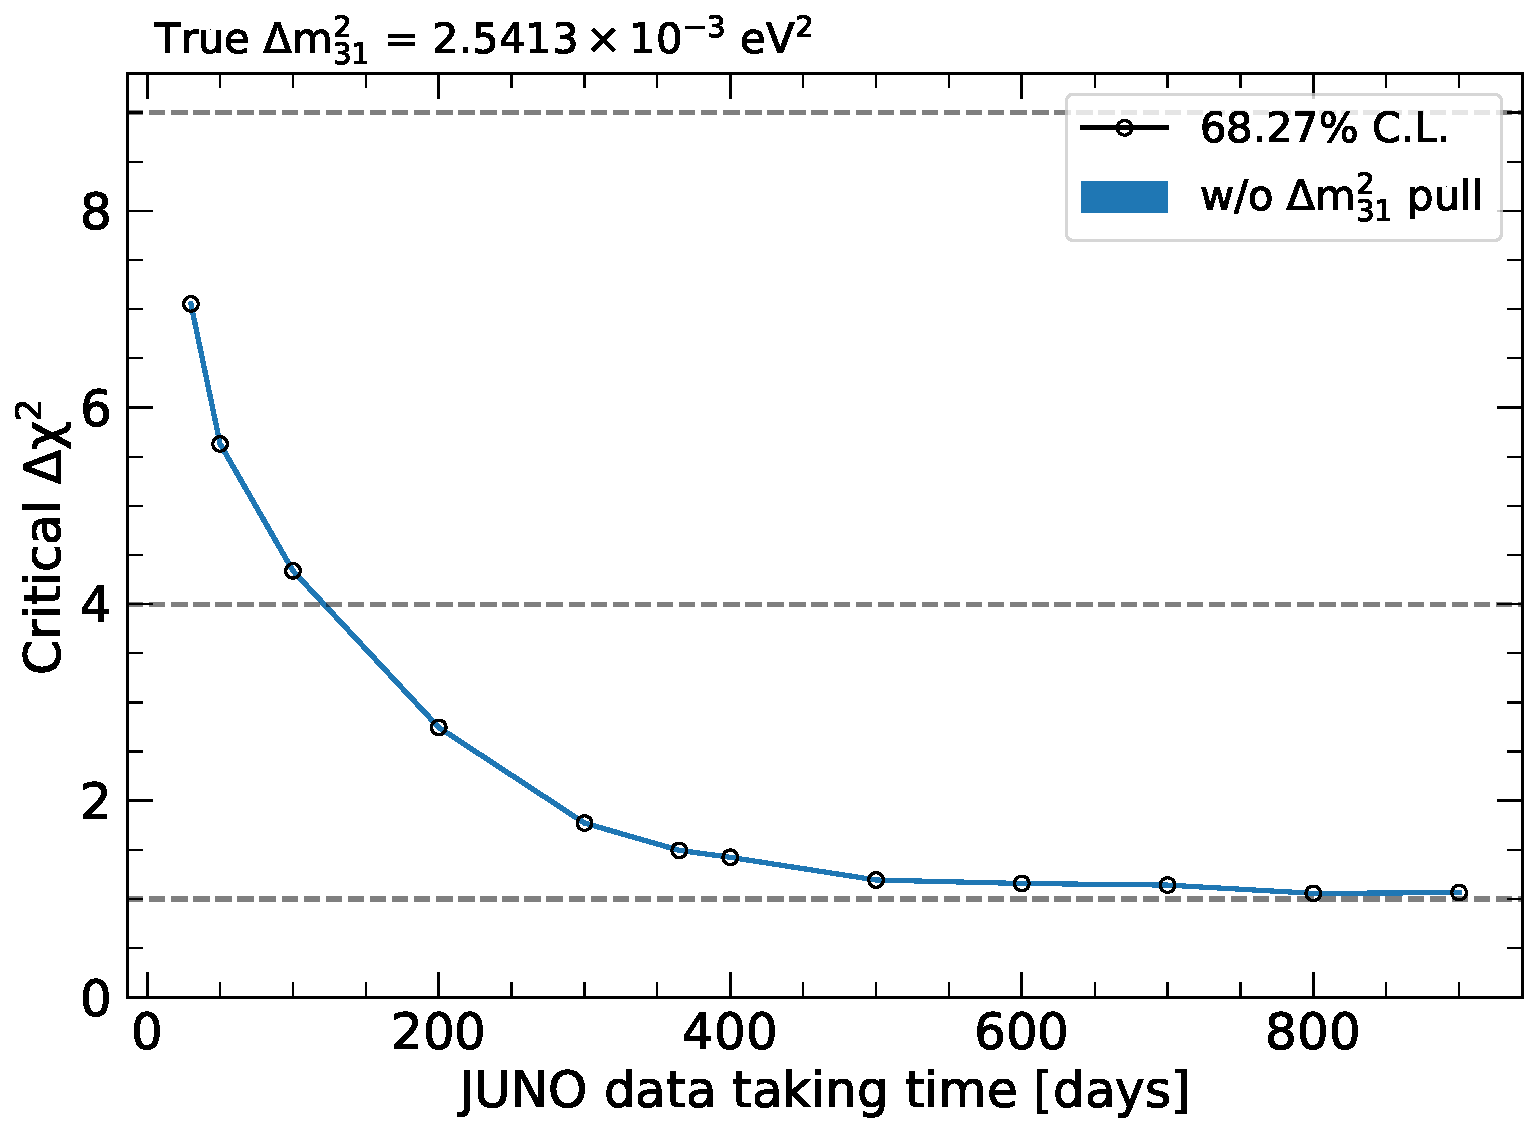
\includegraphics[width=0.7\textwidth]{figs/Section2/han_juno_only_crit_deltachi2_vs_time.pdf}
  \caption{The 68.27\% confidence level critical value ($\Delta\chi^2_{\rm{\rm crit}}$) as a function of JUNO data-taking time.}
  \label{fig:FC_exposure_h}
\end{figure}


\subsection{Dependence on explored $\Delta m^2_{31}$ range}
\begin{figure}[h]
  \begin{subfigure}[t]{0.47\textwidth}
    \centering
    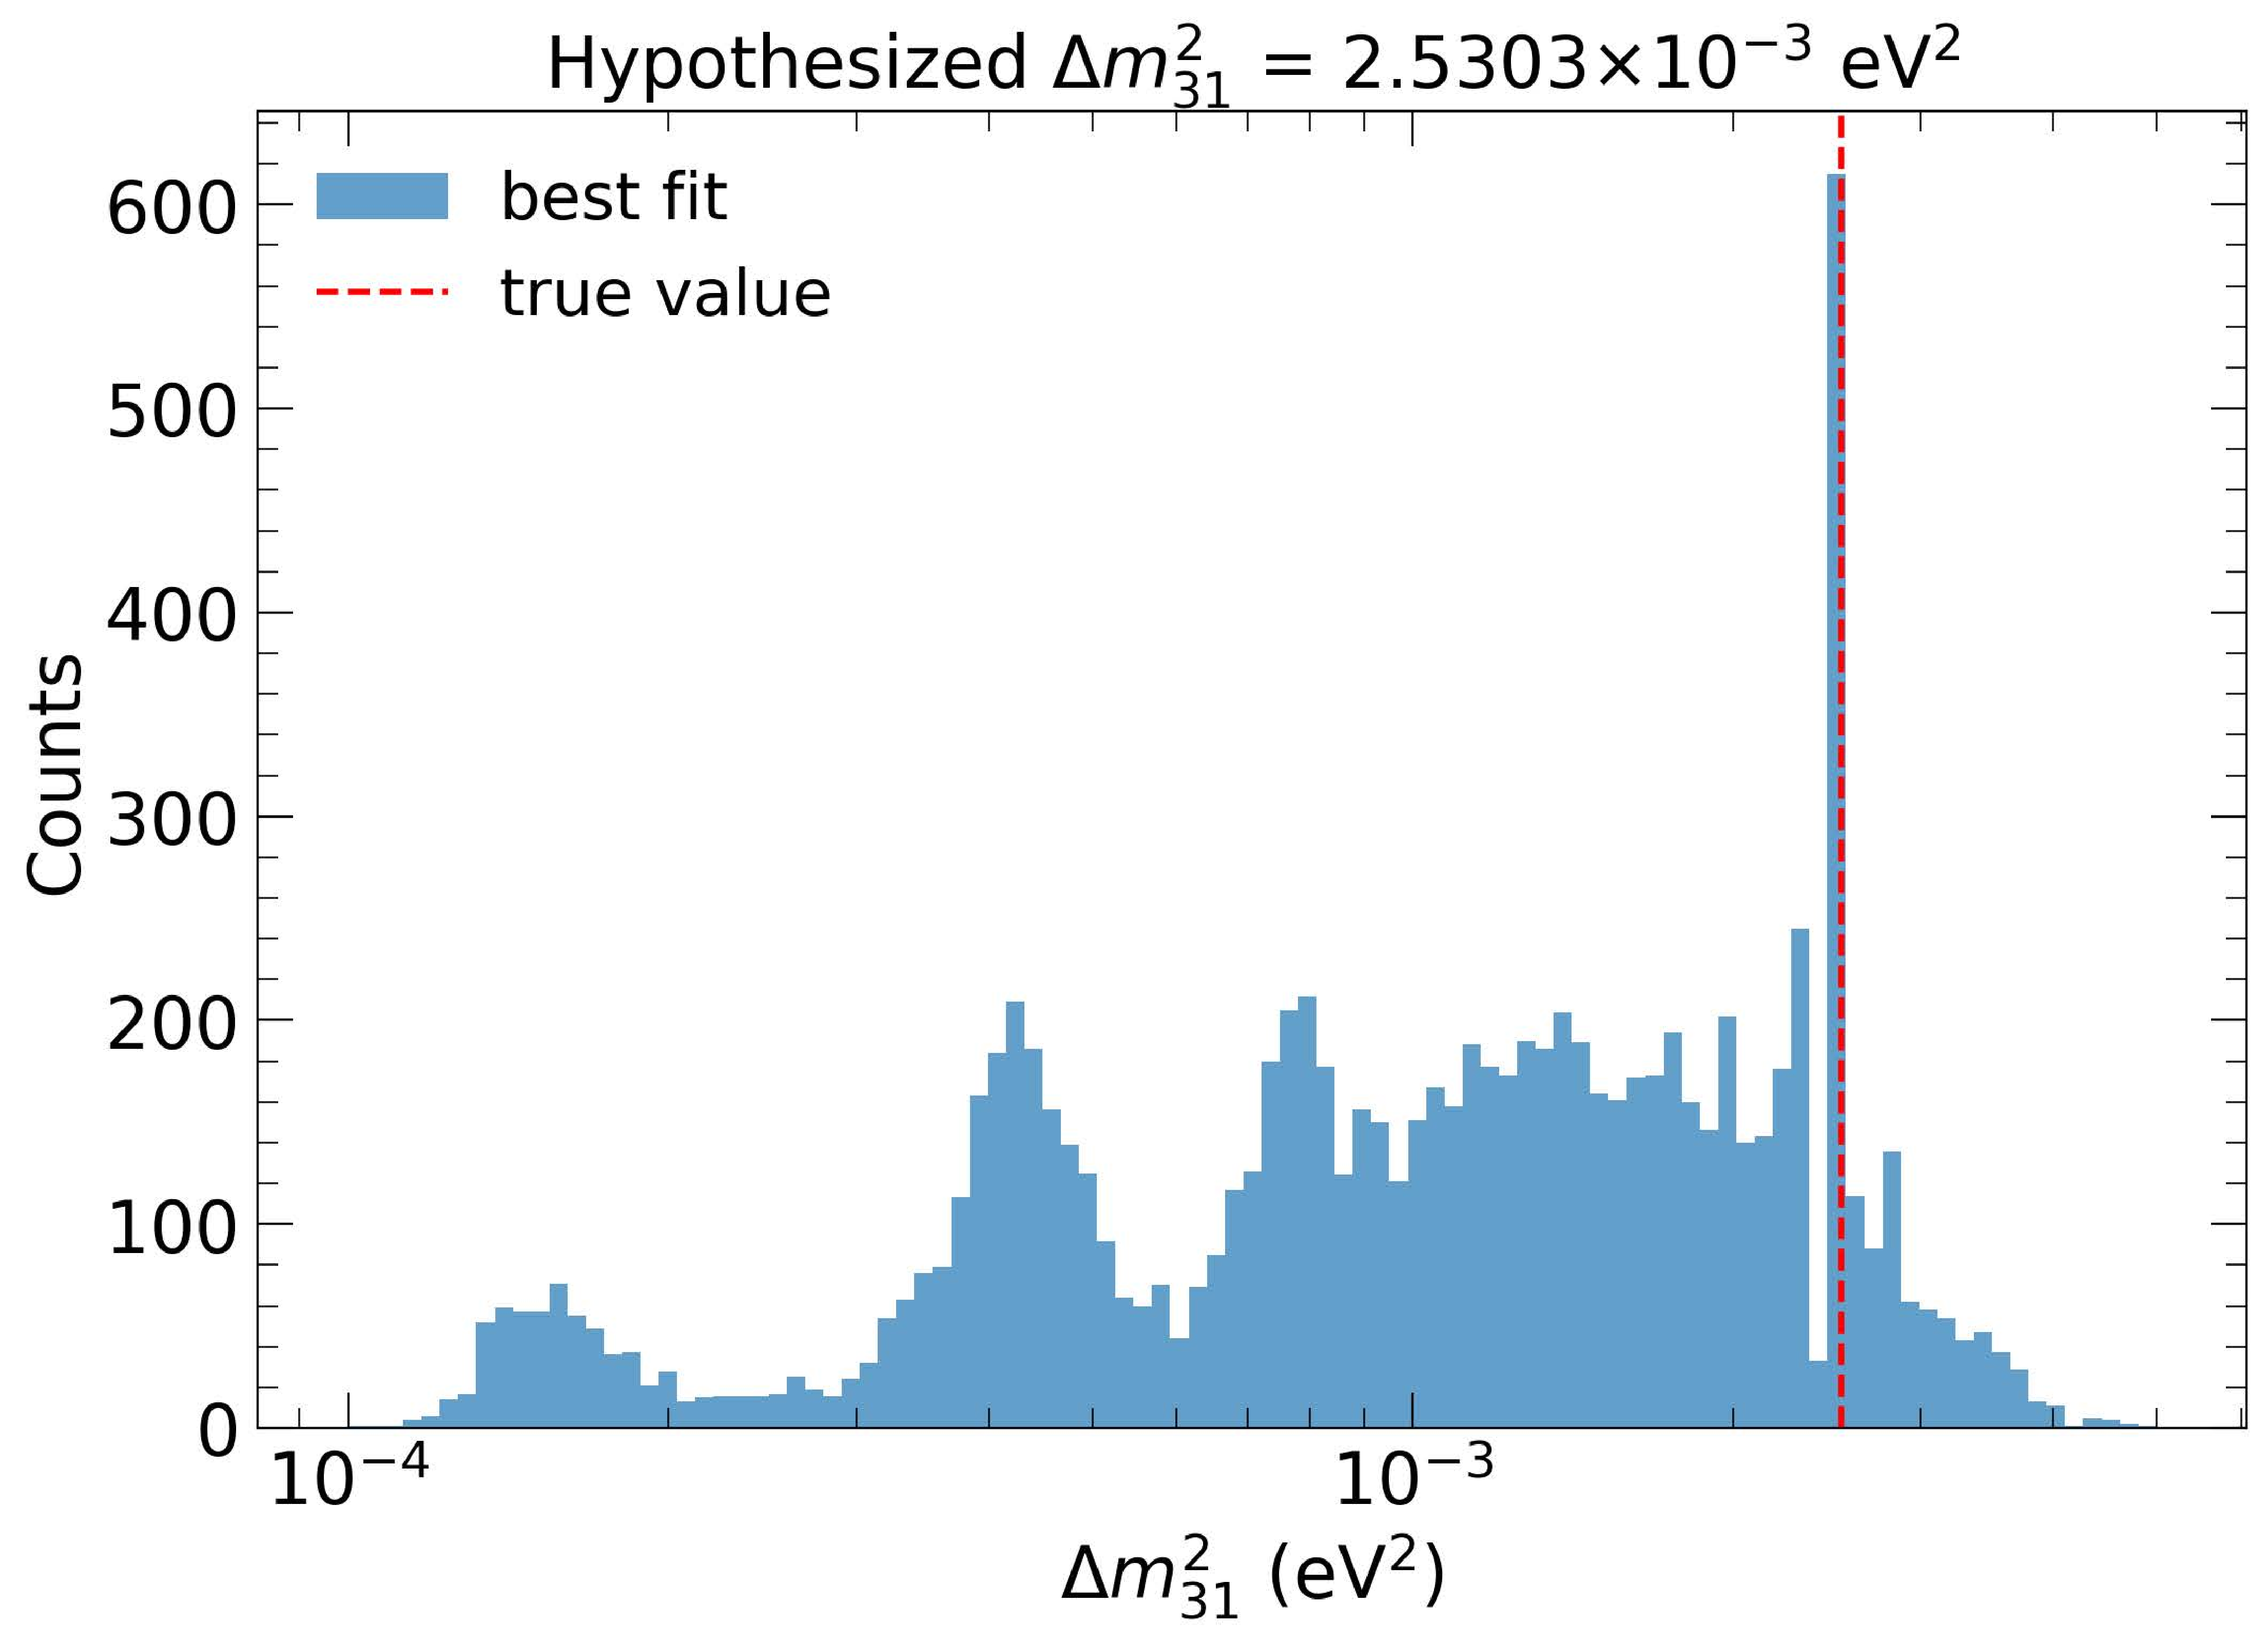
\includegraphics[width=\linewidth]{figs/Section2/Jingqin_dmsq31_bestfit_distribution.pdf}
    \caption{Distribution of Best-Fit $\Delta m^2_{31}$ from Toy MC}
    \label{fig:dmsq31_best_fit_distribution}
  \end{subfigure}
  \hfill
  \begin{subfigure}[t]{0.47\textwidth}
    \centering
    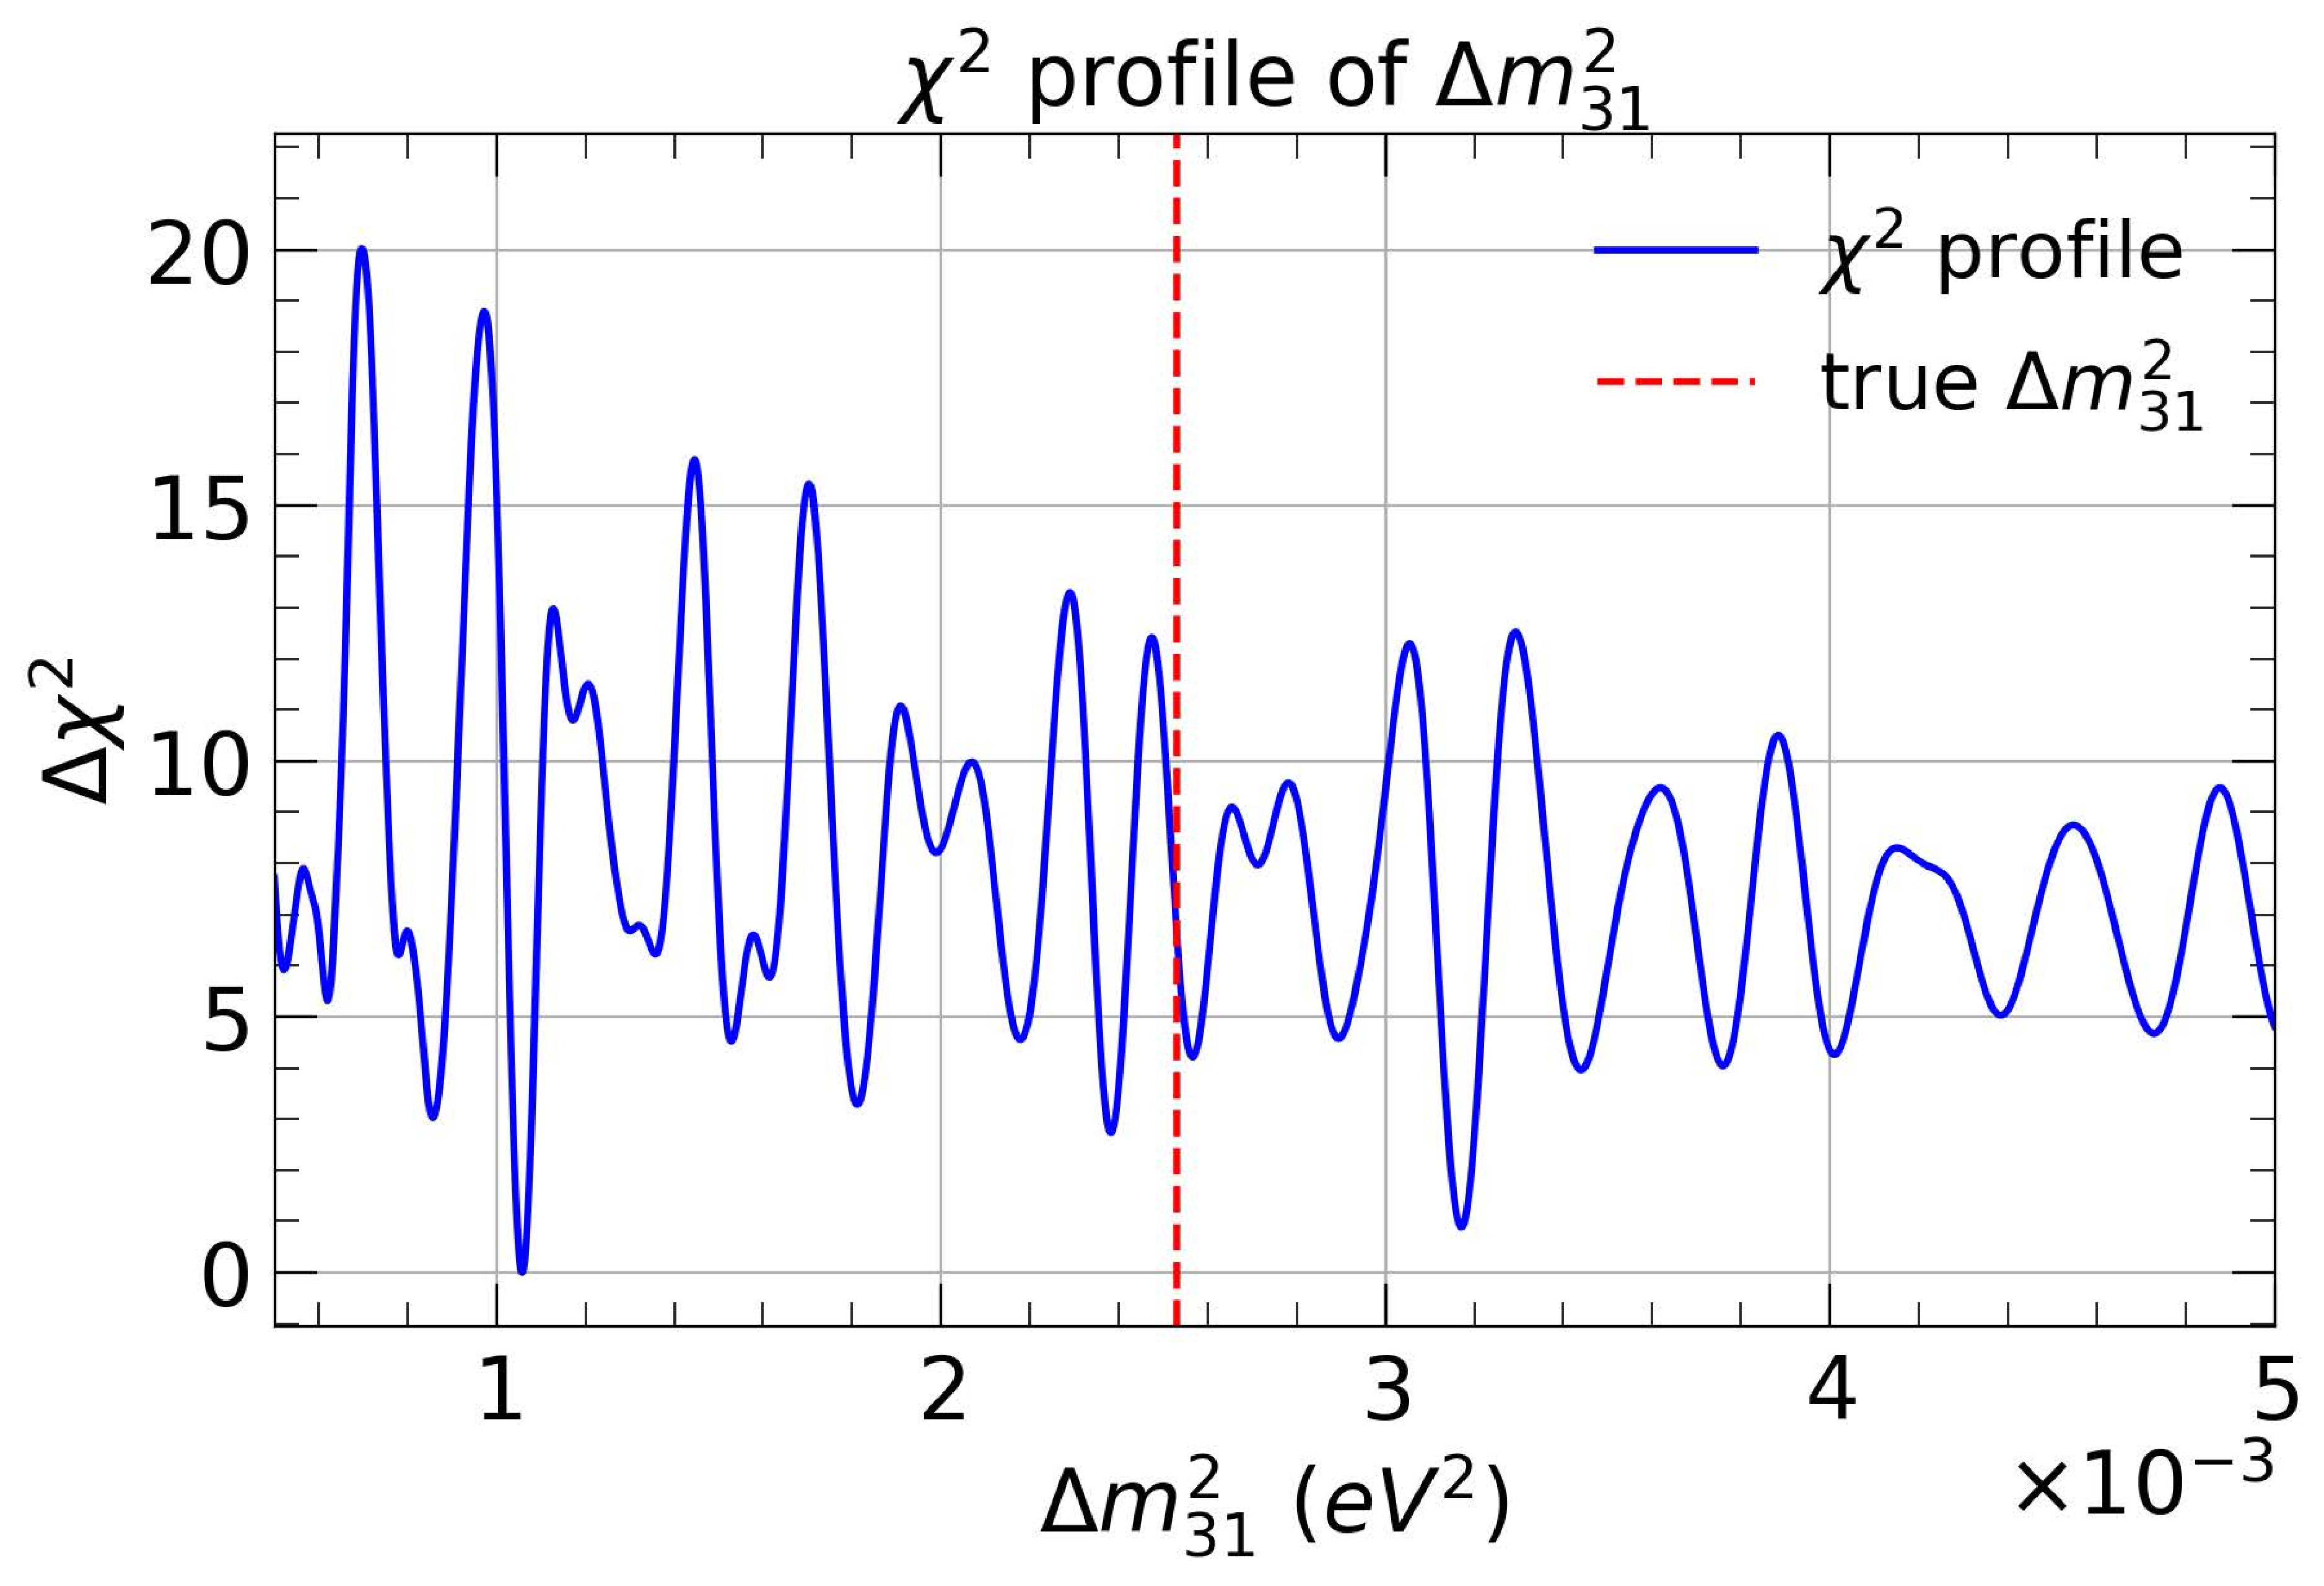
\includegraphics[width=\linewidth]{figs/Section2/Jingqin_toy_data.pdf}
    \caption{$\chi^2$ Profile of $\Delta m^2_{31}$ from a Single Toy Dataset}
    \label{fig:toy_data_profile}
  \end{subfigure}
  \caption{(a)Histogram of best-fit $\Delta m^2_{31}$ values obtained from an ensemble of toy Monte Carlo experiments under 30 days. The horizontal axis shows the best-fit $\Delta m^2_{31}$ (eV$^2$; log scale), and the vertical axis gives the number of best-fit values falling in each bin. The red dashed line marks the true (injected) value. 
(b) $\Delta\chi^2(\Delta m^2_{31})$ profile from a single toy dataset whose global minimum lies far from the true value. The horizontal axis is the scanned $\Delta m^2_{31}$ (eV$^2$); the vertical axis is $\Delta\chi^2$ relative to its minimum. The blue curve exhibits multiple local minima and markedly non-quadratic behavior; the red dashed line denotes the true value.}
  \label{fig:dmsq31_best_fit}
\end{figure}

Under low exposure, \autoref{fig:dmsq31_best_fit} demonstrate that the best-fit values of $\Delta m^2_{31}$ from toy Monte Carlo simulations can deviate substantially from the true value, and the corresponding $\chi^2$ profile for a representative toy is highly non-quadratic and exhibits many local minima. This behavior imply that when constructing the $\Delta \chi^2$ distribution with the Feldman-Cousins method, we must scan the initial guesses for $\Delta m_{31}^2$ over a wide parameter range to ensure the global best fit is found. In practice this requires using broad starting-value intervals (and multiple starting points) during the fit to avoid being trapped in local minima and to guarantee correct coverage in the FC construction.

\begin{figure}[h]
  \begin{subfigure}[t]{0.47\textwidth}
    \centering
    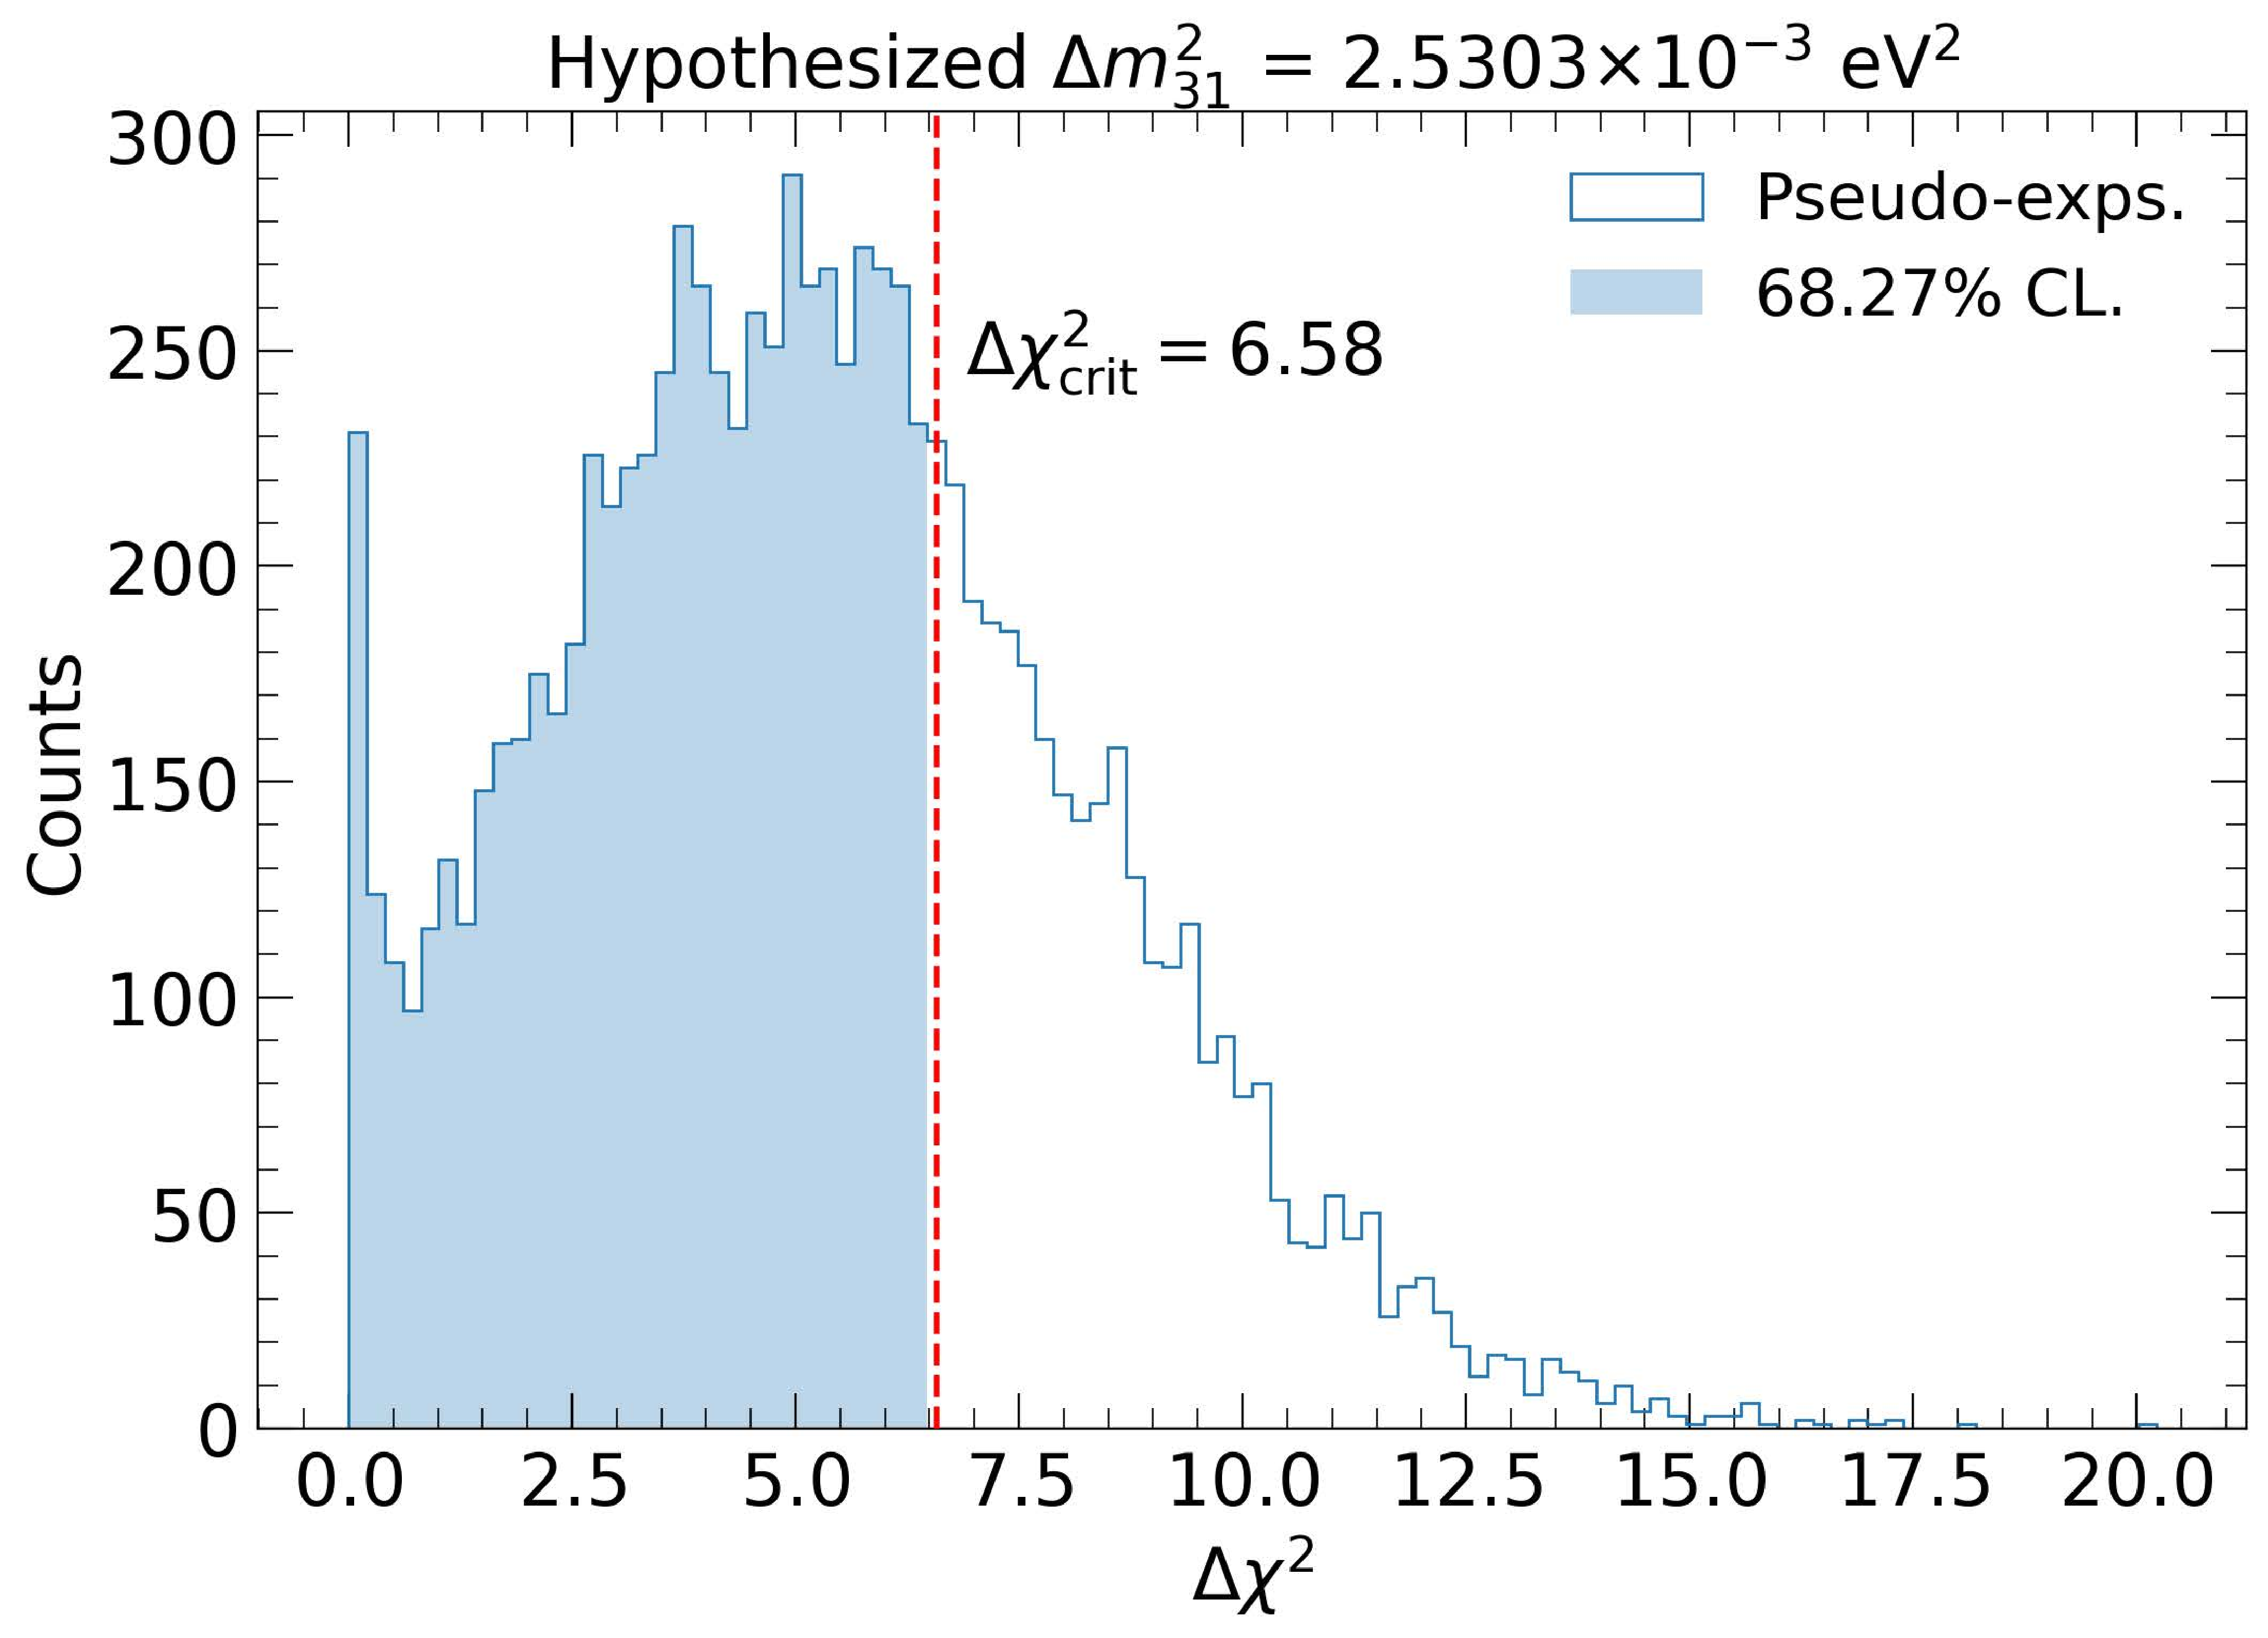
\includegraphics[width=\linewidth]{figs/Section2/Jingqin_big_range_dchi2.pdf}
    \caption{$\Delta m^2_{31} \in [1.0 \times 10^{-4}, 5.0 \times 10^{-3}]$ eV$^2$}
    \label{fig:big_range_dchi2_distribuiton}
  \end{subfigure}
  \hfill
  \begin{subfigure}[t]{0.47\textwidth}
    \centering
    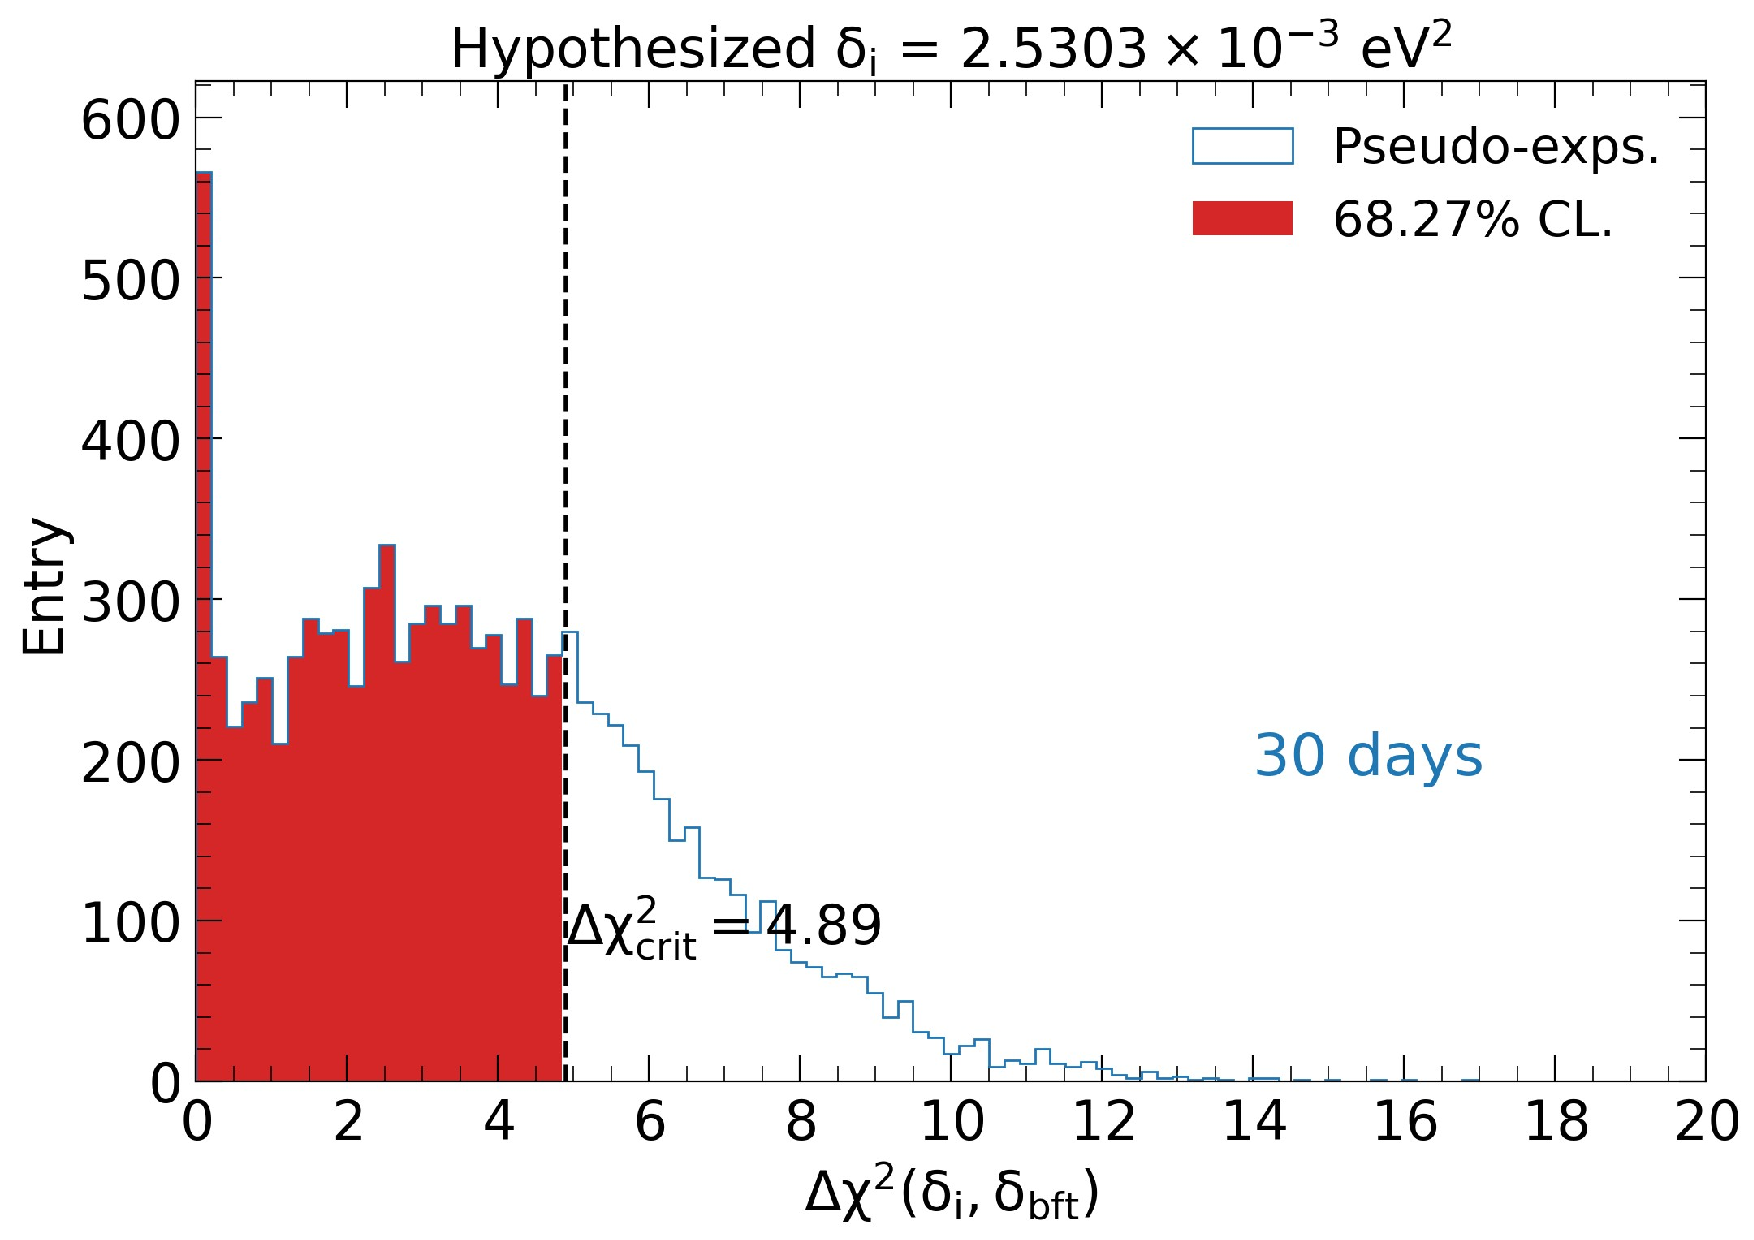
\includegraphics[width=\linewidth]{figs/Section2/Jingqin_small_range_dchi2.pdf}
    \caption{$\Delta m^2_{31} \in [1.5 \times 10^{-3}, 3.5 \times 10^{-3}]$ eV$^2$}
    \label{fig:small_range_dchi2_distribution}
  \end{subfigure}
  \caption{Distribution of the Feldman-Cousins test statistic $\Delta\chi^2$ obtained from pseudo-experiments generated under the hypothesis true value $\Delta m^2_{31} = 2.5303\times10^{-3} \,\mathrm{eV}^2$ (yielding $\Delta\chi^2_{\rm crit}=6.58$). (a) Large scan range: the $\Delta m^2_{31}$ scan was performed over $[1\times10^{-4},\,5\times10^{-3}]\,\mathrm{eV}^2$. (b) Narrow scan range: the $\Delta m^2_{31}$ scan was performed over $[1.5\times10^{-3},\,3.5\times10^{-3}]\,\mathrm{eV}^2$ (yielding $\Delta\chi^2_{\rm crit}=4.89$). The horizontal axis shows the $\Delta\chi^2$ values, and the vertical axis indicates the number of pseudo-experiments yielding a given $\Delta\chi^2$ value. The histogram represents the full distribution from all pseudo-experiments. The shaded blue area marks the central 68.27\% quantile range, corresponding to the one-standard-deviation ($1\sigma$) confidence level in the Feldman–Cousins construction. The vertical dashed line indicates the conventional $\Delta\chi^2 = 1$ threshold assumed under Wilks’ theorem. }
  \label{fig:dmsq31_dchi2_distribution}
\end{figure}

For each pseudo-experiment, we define $\Delta\chi^2$ as the difference between the $\chi^2$ evaluated at the hypothesized value $\Delta m^2_{31}=2.5303\times10^{-3}\,\mathrm{eV}^2$ and the global minimum $\chi^2$ from an unconstrained fit. \autoref{fig:dmsq31_dchi2_distribution} demonstrates that, in this low-statistics regime, the conventional Wilks threshold $(\Delta\chi^2=1)$ substantially underestimates the true uncertainty: the Feldman–Cousins critical value obtained from pseudo-experiments can be much larger. Moreover, the chosen scan interval for $\Delta m^2_{31}$ materially affects the FC critical value. With a narrow scan $[1.5\times10^{-3},\,3.5\times10^{-3}]\,\mathrm{eV}^2$ we find $\Delta\chi^2_{\rm crit}=4.89$, whereas extending the range to $[1.0\times10^{-4},\,5.0\times10^{-3}]\,\mathrm{eV}^2$ raises the critical value to $\Delta\chi^2_{\rm crit}=6.58$. This behavior arises because a too-restricted scan can miss alternative global minima, producing artificially small $\Delta\chi^2$ values for some toys and hence undercoverage. Therefore, when building FC intervals at low exposure one must scan a sufficiently wide parameter range (and use multiple starting points) to ensure the global minimum is found and the resulting confidence intervals have correct coverage.

\subsection{Conclusions of this Section}
The low statistics measurement of $\Delta m^2_{31}$ poses a range of challenges:
\begin{itemize}
    \item Wilks' theorem cannot be used until a certain exposure (order of 2 years) because it produces significant undercoverage. The profiled Feldman-Cousin method, as applied by the NO$\nu$A collaboration~\cite{NOvA:2022wnj} seems to be a viable option to get the right coverage properties while properly accounting for nuisance parameters. It is worth mentioning that applying a full profiled FC procedure requires a large amount of computational power.
    This computational burden becomes particularly severe for the FC procedure, which requires thousands of pseudoexperiments. For final physics results the full profiled FC approach remains the suggested option despite its computational demands.
    \item The FC method provides more conservative confidence intervals compared to Wilks' theorem, with empirical critical values that are 3-7 times larger than asymptotic predictions depending on exposure level. This conservative nature means that the "bad minima" situation described in \autoref{sec:2_bad_minima} becomes even more pronounced when using statistically rigorous methods.
    \item According to our results, there is a very high probability of obtaining disjoint $1\sigma$ confidence intervals during the first months of data taking, with 97\% of measurements at 50 days and 87\% at 100 days exhibiting multiple disconnected confidence regions. This situation improves significantly after one year of data taking, when only 13\% of measurements show interval degeneracy. This timeline coincides with when JUNO will likely have accumulated enough statistics to get a meaningful neutrino mass ordering determination in combination with long-baseline experiments, as will be discussed in the following section. 
    \item Multiple disjoint intervals are still present after one year if considering the $2\sigma$ and $3\sigma$ confidence levels.
    \item Results at low statistics exhibit strong dependence on the chosen range of $\Delta m_{31}^2$ used in our FC studies.  While a large part of the parameter space is excluded based on other experiments measurements, the likelihood function does not go to zero in these regions, leading to artificial parameter degeneracies that can only be resolved with increased exposure. This range dependence means that early JUNO results will be particularly sensitive to the choice of parameter boundaries for $\Delta m_{31}^2$, i.e. the range over which the grid scan is performed to search for the global minimum (for example, $\Delta m^2_{31} \in [1.5 \times 10^{-3},3.5 \times 10^{-3}]\mathrm{~eV}^2$ in Fig.~\ref{fig:dmsq31_dchi2_distribution}), raising the question of what boundaries to use.  

\end{itemize}

\clearpage
\section{Measurement of solar parameters at low exposure}\label{sec:solar_params}
In this section we cover the measurement of solar neutrino oscillation parameters $\Delta m^2_{21}$ and $\sin^2\theta_{12}$ at low statistics. 
The same configuration mentioned in \autoref{sec:coverage} is used to generate toys. In particular, for the following results we use the combined Person-Neyman $\chi^2_{\mathrm{CNP}}$ for Asimov results and $\chi^2_{\mathrm{P}}+\ln(|V|)$  (Pearson + log-correction) for pseudoexperiments. This choice aims at reducing biases in oscillation parameters.

\subsection{Toy MC study}
20,000 pseudo-experiments are generated with nominal value of both oscillation and nuisance parameters, including statistical and systematical fluctuations, for several exposures. 
\autoref{fig:dm2_21_low_stat_BFV} shows the distribution of $\Delta m^2_{21}$ best-fit values for 30, 50, and 100 days exposure. The toy MC results are compared with Asimov results. The blue marker represents the confidence interval obtained using the symmetric 68.27\% integral method. All best-fit values are sorted in ascending order and then the 15.865th percentile and 84.135th percentile of the distribution are calculated. The violet marker and curve are obtained from a fit on an Asimov dataset with the same input values, taking the best fit value and uncertainties provided by the minimization algorithm and assuming perfect Gaussian behavior. 
\autoref{fig:dm2_21_low_stat_BFV} shows excellent agreement between the empirical distributions and the theoretical Gaussian predictions at all tested exposure levels. The violet curves closely follow the histograms, indicating that $\Delta m^2_{21}$ measurements remain well behaved even with limited statistics.

\autoref{fig:s12_low_stat_BFV} shows the distribution of best-fit values for $\sin^2 \theta_{12}$ at 30, 50, and 100 days of exposure. While $\sin^2 \theta_{12}$ behaves similarly to $\Delta m^2_{21}$, a noticeable bias appears at 30 days. However, this bias is already significantly reduced at 50 days. Moreover, as discussed later, alternative binning strategies can help further minimize this effect.

\begin{figure}[ht]
  \centering
  \begin{subfigure}[t]{0.32\textwidth}
    \centering
    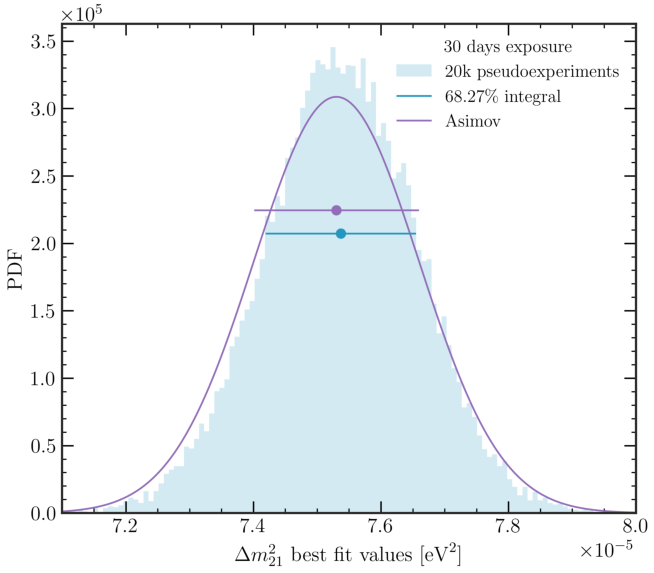
\includegraphics[width=\linewidth]{figs/Section2/vanessa_dm21_30d.pdf}
    \caption{30 days exposure}
    \label{fig:dm2_21_30d}
  \end{subfigure}
  \hfill
  \begin{subfigure}[t]{0.32\textwidth}
    \centering
    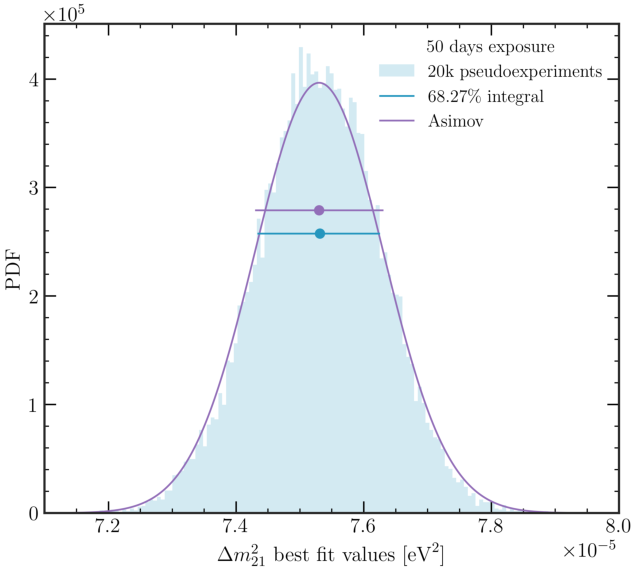
\includegraphics[width=\linewidth]{figs/Section2/vanessa_dm21_50d.pdf}
    \caption{50 days exposure}
    \label{fig:dm2_21_50d}
  \end{subfigure}
\hfill
  \begin{subfigure}[t]{0.32\textwidth}
    \centering
    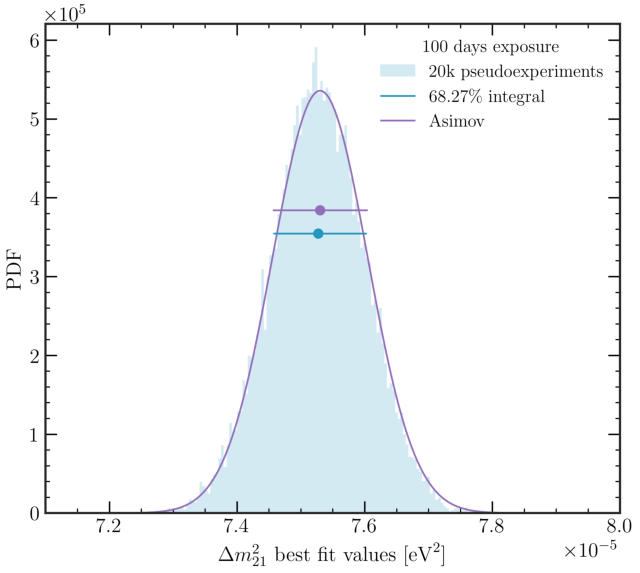
\includegraphics[width=\linewidth]{figs/Section2/vanessa_dm21_100d.pdf}
    \caption{100 days exposure}
    \label{fig:dm2_21_100d}
  \end{subfigure}
  \caption{Distribution of $\Delta m^2_{21}$ best-fit values from 20,000 pseudoexperiments at low exposures.}
  \label{fig:dm2_21_low_stat_BFV}
\end{figure}



\begin{figure}[H]
  \centering
  \begin{subfigure}[t]{0.32\textwidth}
    \centering
    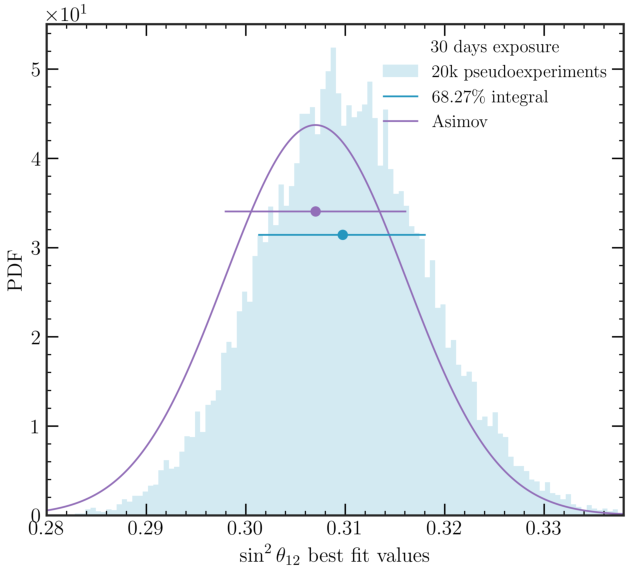
\includegraphics[width=\linewidth]{figs/Section2/vanessa_s12_30d.pdf}
    \caption{30 days exposure.}
    \label{fig:s12_30d}
  \end{subfigure}
  \hfill
  \begin{subfigure}[t]{0.32\textwidth}
    \centering
    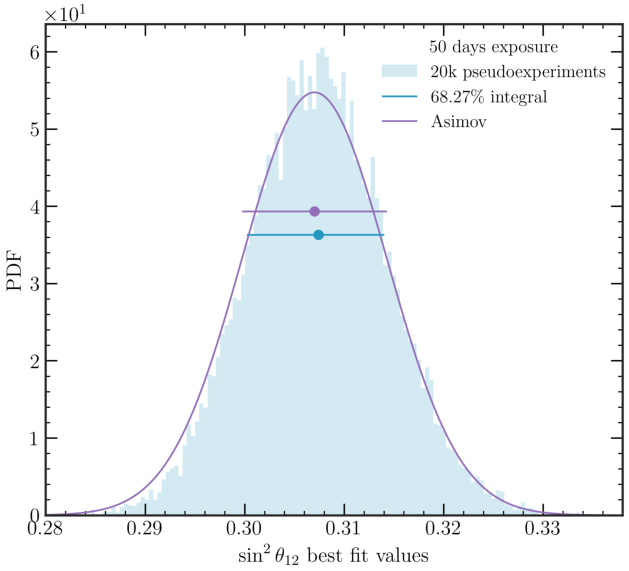
\includegraphics[width=\linewidth]{figs/Section2/vanessa_s12_50d.pdf}
    \caption{50 days exposure.}
    \label{fig:s12_50d}
  \end{subfigure}
\hfill
  \begin{subfigure}[t]{0.32\textwidth}
    \centering
    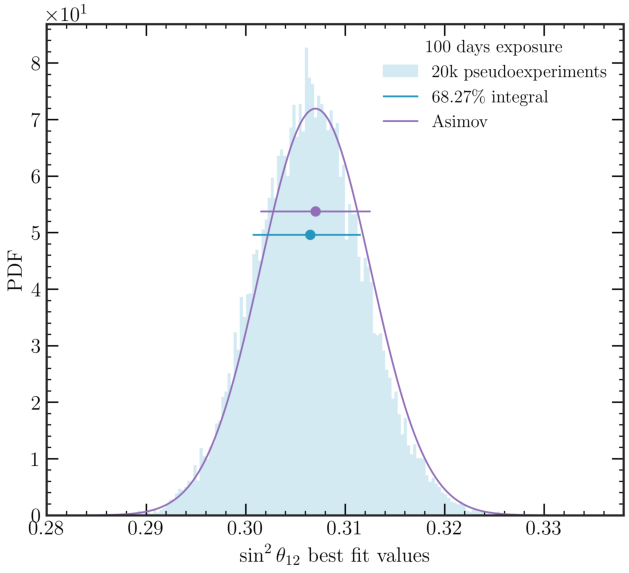
\includegraphics[width=\linewidth]{figs/Section2/vanessa_s12_100d.pdf}
    \caption{100 days exposure.}
    \label{fig:s12_100d}
  \end{subfigure}
  \caption{Distribution of $\sin^2 \theta_{12}$ best-fit values from 20,000 pseudoexperiments at low exposures. }
  \label{fig:s12_low_stat_BFV}
\end{figure}

\subsubsection{Evolution of bias and precision}
When working with low statistics data, some bins in the spectrum may contain very few counts, or even none at all. In such cases, the chi-squared test statistic becomes unreliable. This, in turn, can introduce biases in parameter estimates. A practical way to reduce this bias is to use broader bins either in regions of the spectrum where event counts are expected to be low, or in the full range considered. The effect of changing the bin size is explored in \autoref{sec:binning_solar}. The following results are obtained with the nominal binning, i.e, 20 keV wide bins.

\autoref{fig:solar_low_stat_bias} and \autoref{fig:solar_low_stat_precision} present the temporal evolution of bias and precision for both solar oscillation parameters. 

The bias for each parameter is calculated as the normalized difference between the mean of the best-fit value distribution and the true input value: 
\begin{equation}
    \text{Bias} = \frac{\langle\hat{\theta}\rangle - \theta_{\text{true}}}{\sigma_{\text{68\%}}},
\end{equation}
where $\langle\hat{\theta}\rangle$ represents the mean of the best-fit values from 20,000 pseudoexperiments, $\theta_{\text{true}}$ is the nominal input parameter value, and $\sigma_{\text{68\%}}$ is the uncertainty estimated from the aforementioned distribution. \autoref{fig:solar_low_stat_bias} highlights a difference in bias behavior between the two solar parameters. For $\Delta m^2_{21}$, the bias remains consistently below $0.1\sigma$ across all exposure levels. In contrast, $\sin^2\theta_{12}$ displays a more noticeable bias of approximately $0.3\sigma$ at 30 days, which decreases significantly with increased exposure and becomes minimal by 100 days. 


\autoref{fig:solar_low_stat_precision} shows a fairly good agreement between empirical Toy MC results and theoretical Asimov precision estimates for both solar parameters. The projected JUNO precision allows for a significant improvement over current global constraints reported by NuFit 6.0~\cite{Nufit:2024eli}. Specifically, for $\Delta m^2_{21}$, NuFit quotes a relative uncertainty of about 2.5\%, while JUNO achieves a precision of approximately 1.6\% with just 30 days of exposure. Similarly, for $\sin^2\theta_{12}$, the global fit uncertainty is around 3.9\%, whereas JUNO has a projected precision of about 2.7\% at the same exposure level. It is worth noting that these results are obtained under the assumption of nominal systematic uncertainties, i.e., with excellent knowledge of the nuisance parameters. In practice, such control of systematic uncertainties (specifically, detector response, background estimation, etc.) is unlikely to be achieved with only 50 days of data. For a more realistic scenario, including the impact of looser systematic constraints, we refer to the presentation in Ref.~\cite{docdb:julyCMtfreport} given at the July 2025 collaboration meeting, where the effect of relaxing these assumptions was discussed.

\begin{figure}[ht]
  \centering
  \begin{subfigure}[t]{0.47\textwidth}
    \centering
    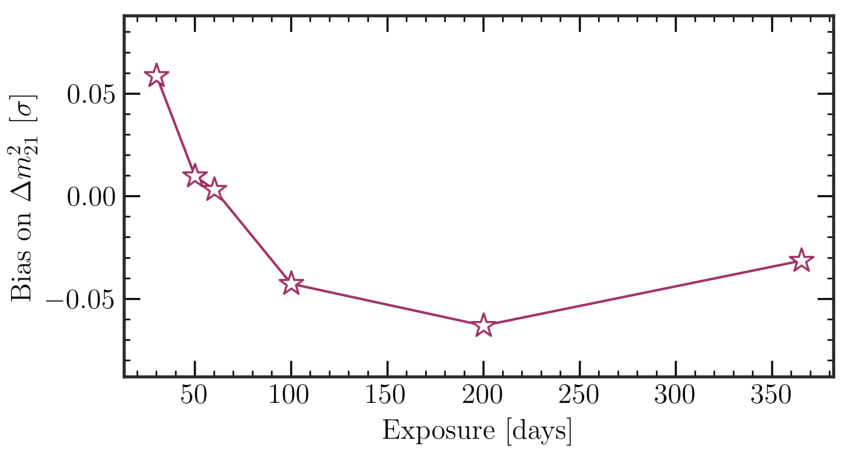
\includegraphics[width=\linewidth]{figs/Section2/vanessa_bias_dm21.pdf}
    \caption{$\Delta m^2_{21}$ bias evolution.}
    \label{fig:dm2_21_bias}
  \end{subfigure}
  \hfill
  \begin{subfigure}[t]{0.47\textwidth}
    \centering
    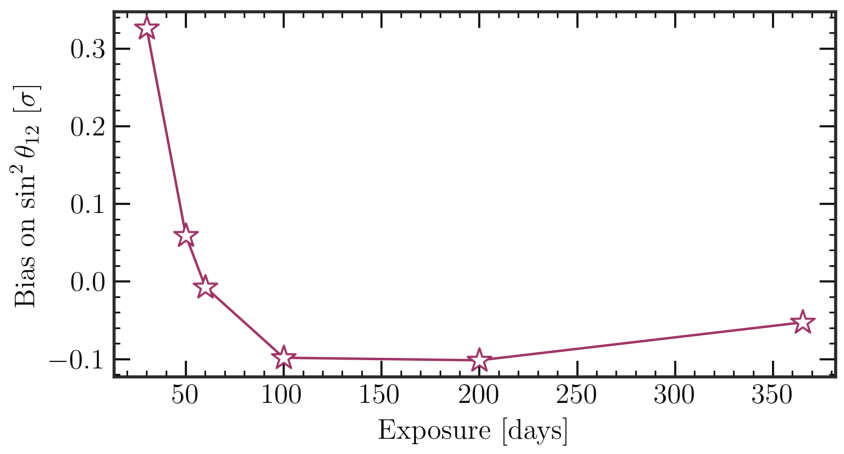
\includegraphics[width=\linewidth]{figs/Section2/vanessa_bias_s12.pdf}
    \caption{$\sin^2\theta_{12}$ bias evolution.}
    \label{fig:s12_bias}
  \end{subfigure}
  \caption{Evolution of bias for solar oscillation parameters as function of exposure time.}
  \label{fig:solar_low_stat_bias}
\end{figure}


\begin{figure}[ht]
  \centering
  \begin{subfigure}[t]{0.47\textwidth}
    \centering
    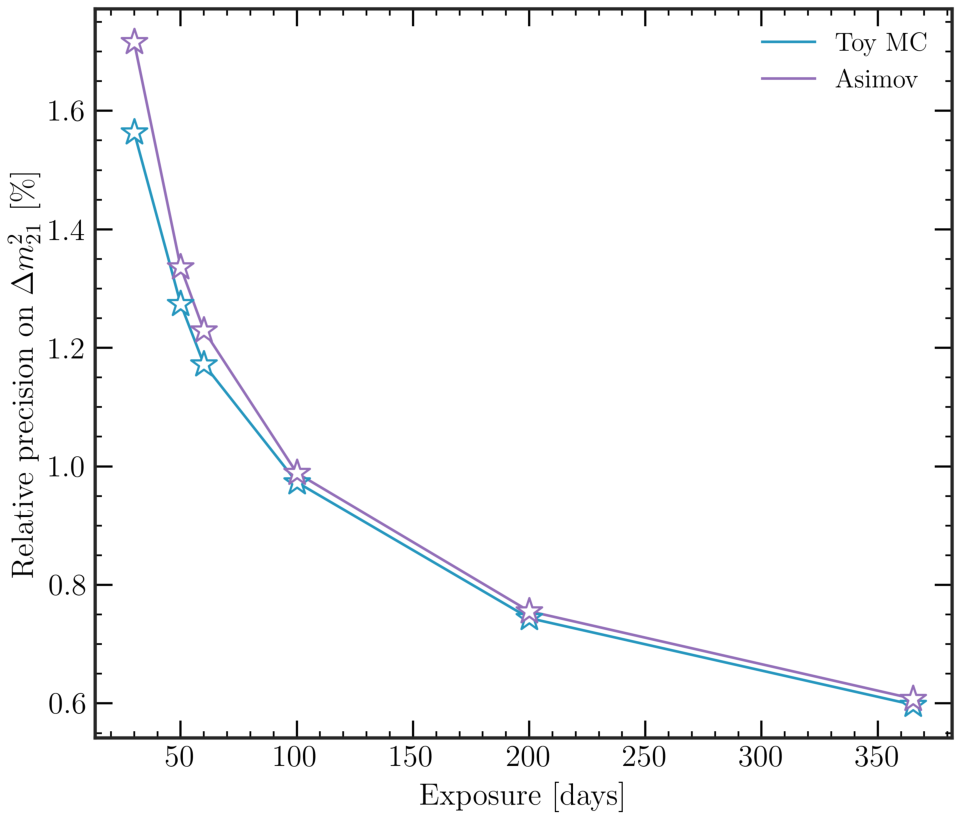
\includegraphics[width=\linewidth]{figs/Section2/vanessa_precision_dm21.pdf}
    \caption{$\Delta m^2_{21}$ precision as a function of exposure.}
    \label{fig:dm2_21_precision}
  \end{subfigure}
  \hfill
  \begin{subfigure}[t]{0.47\textwidth}
    \centering
    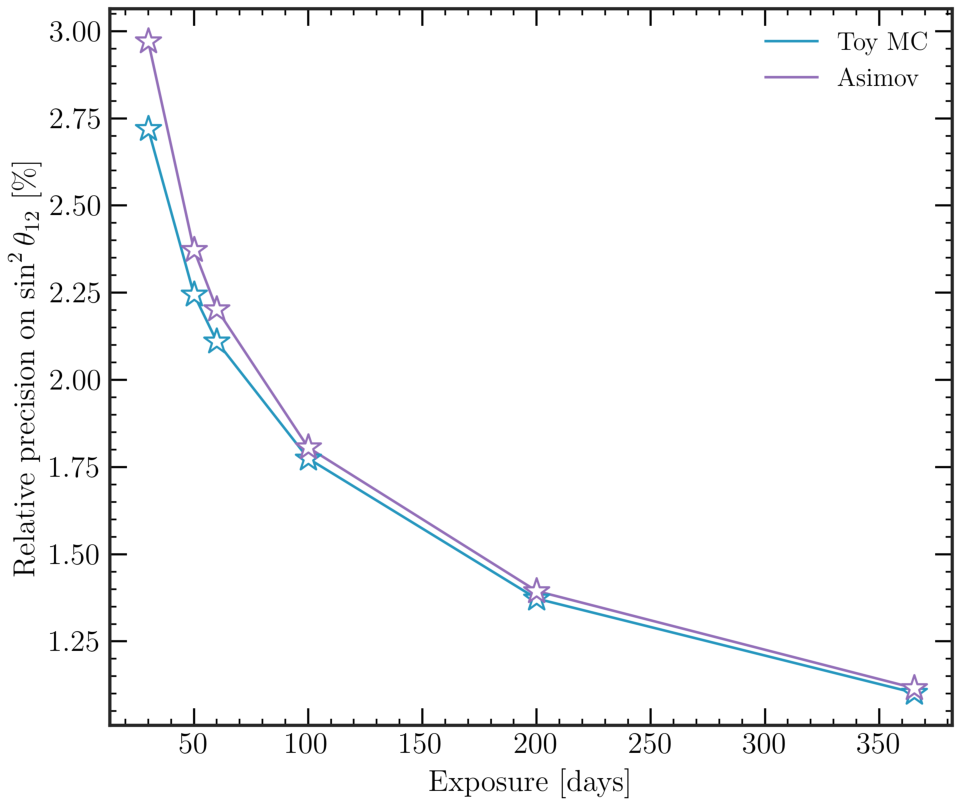
\includegraphics[width=\linewidth]{figs/Section2/vanessa_precision_s12.pdf}
    \caption{$\sin^2\theta_{12}$ precision as a function of exposure. }
    \label{fig:s12_precision}
  \end{subfigure}
  \caption{Evolution of precision for solar oscillation parameters as function of exposure time.}
  \label{fig:solar_low_stat_precision}
\end{figure}

\subsection{Binning strategy}\label{sec:binning_solar}
To investigate and mitigate the observed bias, particularly in $\sin^2\theta_{12}$ measurements at low exposure, an independent analysis was carried out. The study specifically examined how changing binning configurations influence the bias at 30 days of exposure, where the effect is most significant. Three different binning schemes using 10,000 pseudoexperiments are investigated:

\begin{itemize}
    \item \textbf{560 bins} from 0.2 to 12 MeV, matching the nominal binning used in the previous sections. 
    \item \textbf{80 bins} from 0.2 to 12 MeV, i.e., a rebin factor of 7.
    \item \textbf{56 bins} from 0.2 to 12 MeV, i.e., a rebin factor of 10.
\end{itemize}

\autoref{fig:s12_binning} shows the distribution of $\sin^2\theta_{12}$ best-fit values from these studies. The results demonstrate a clear bias reduction as the number of bins decreases.


\begin{figure}[h!]
  \centering
  \begin{subfigure}[t]{0.32\textwidth}
    \centering
    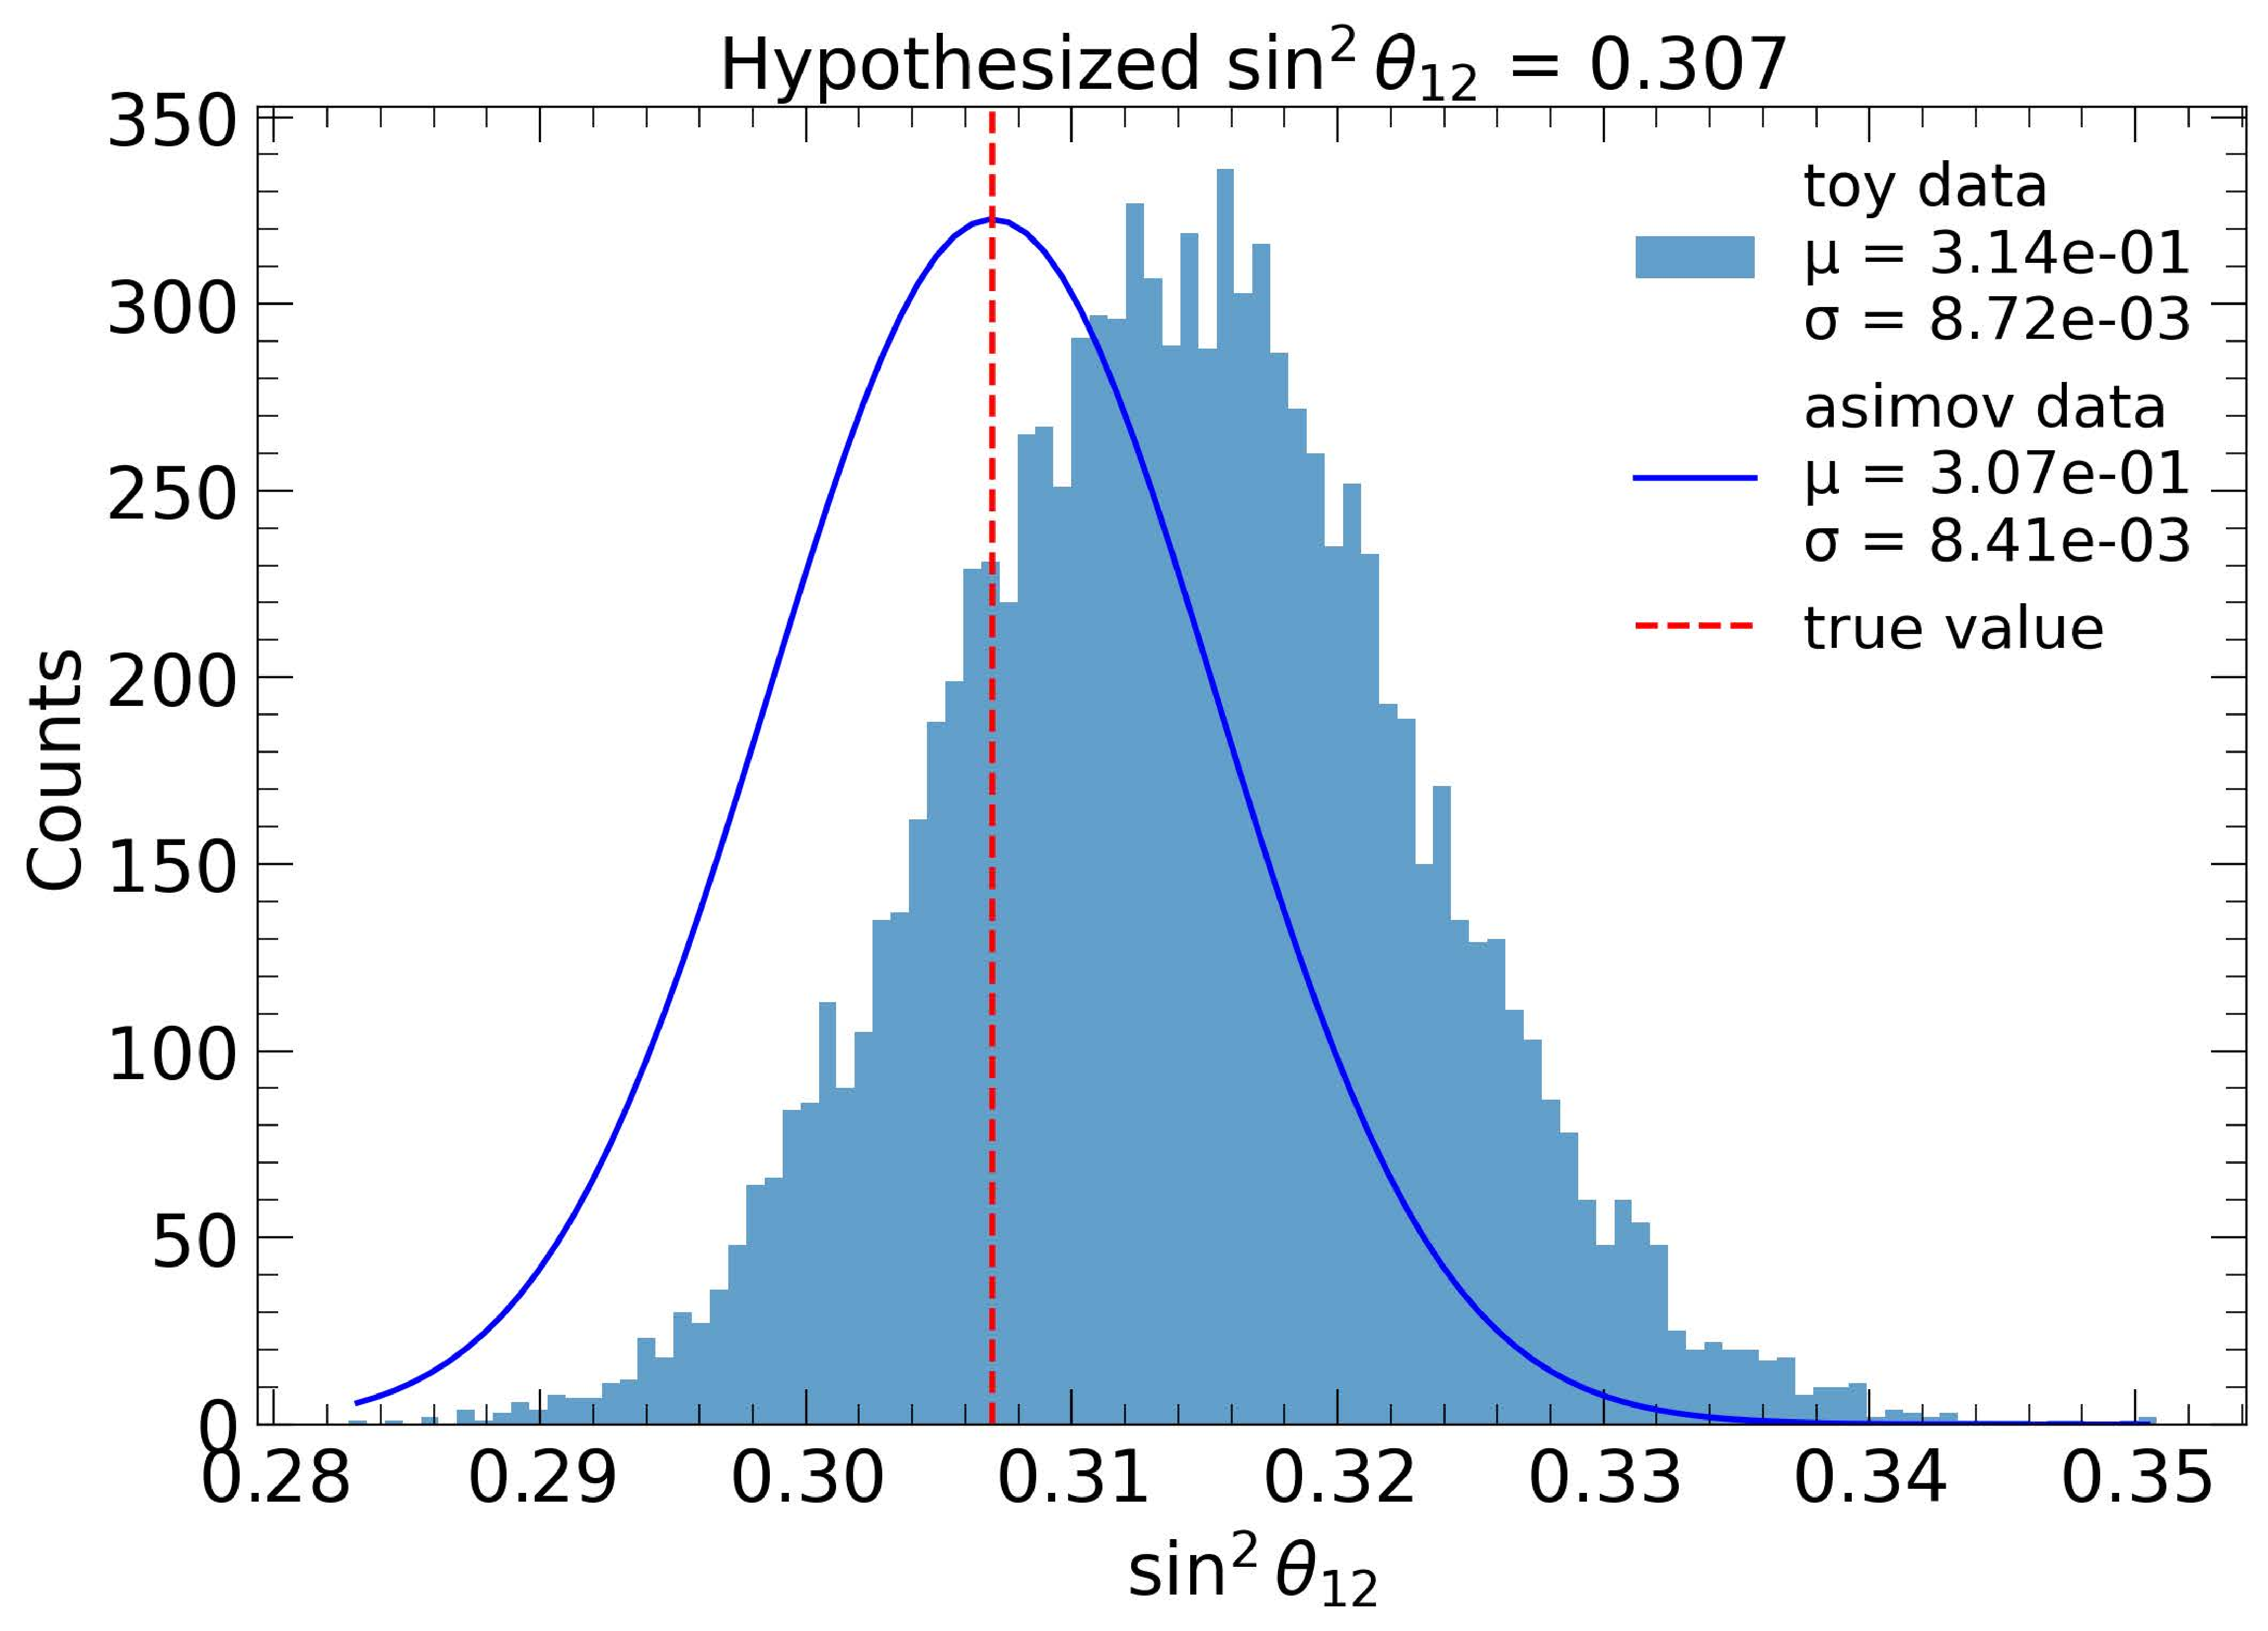
\includegraphics[width=\linewidth]{figs/Section2/Jingqin_sinsq12_bias_560bins.pdf}
    \caption{560 bins.}
    \label{fig:s12_binning_nominal}
  \end{subfigure}
  \hfill
  \begin{subfigure}[t]{0.32\textwidth}
    \centering
    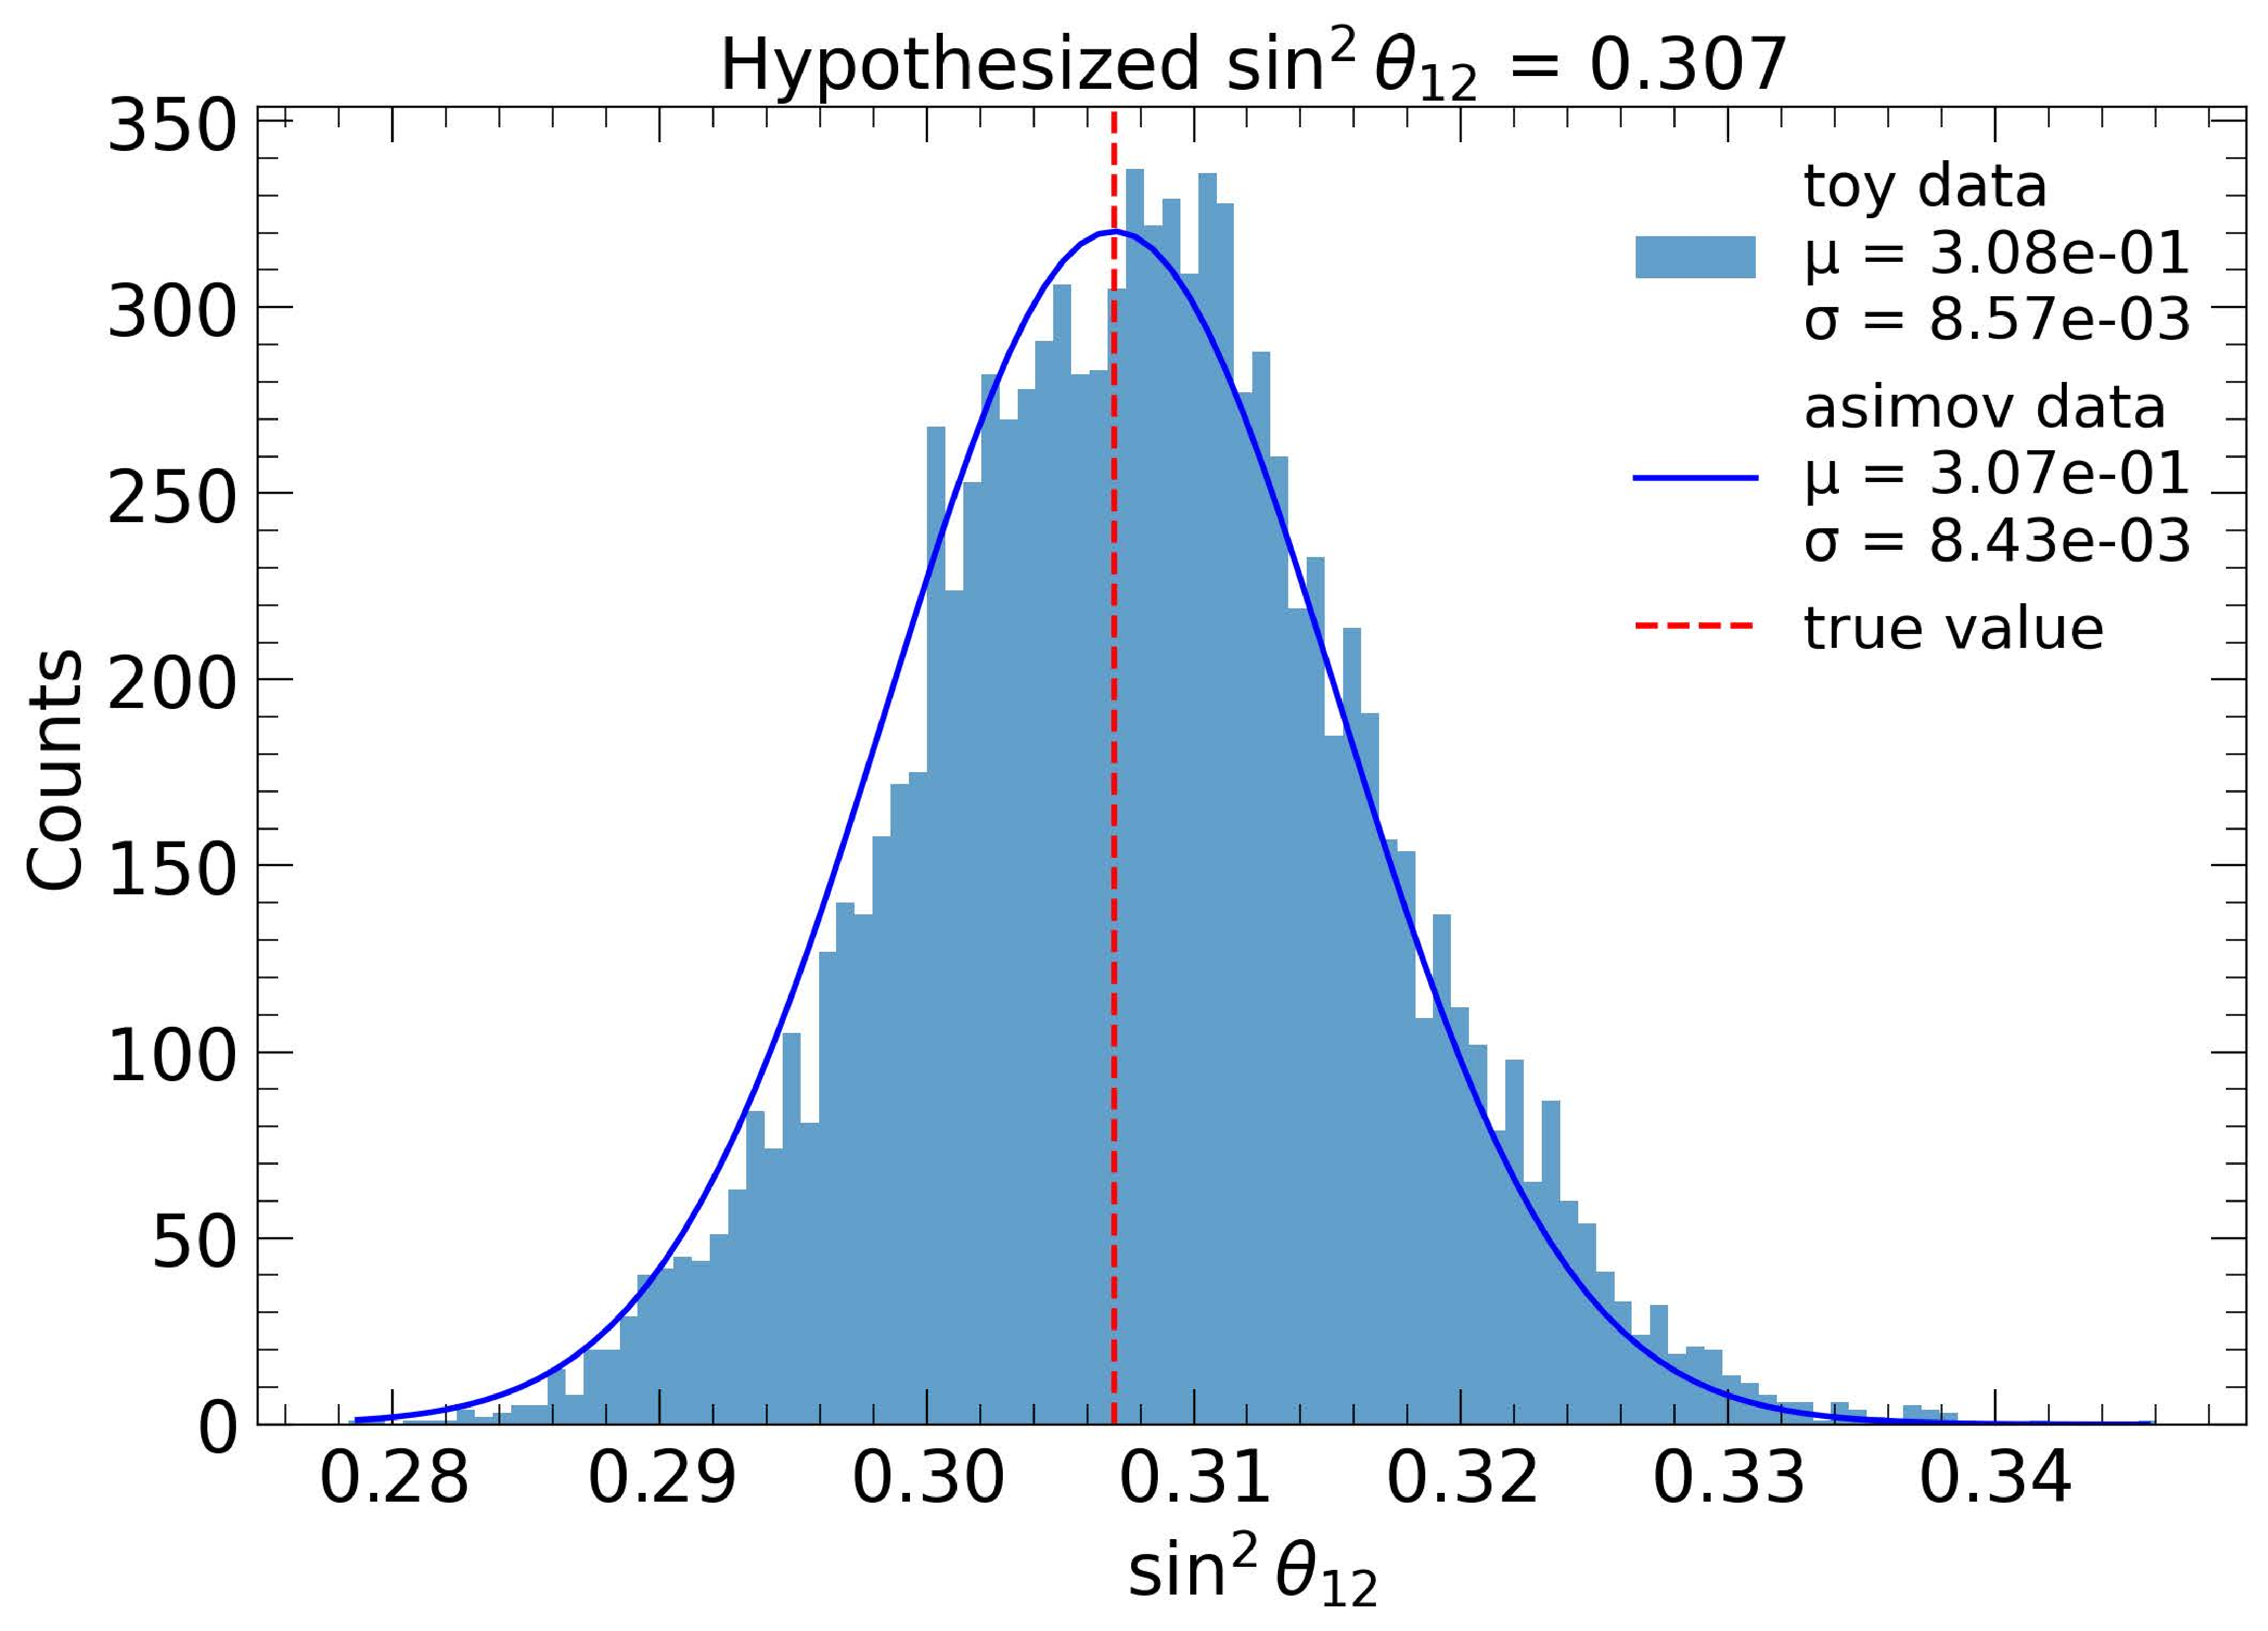
\includegraphics[width=\linewidth]{figs/Section2/Jingqin_sinsq12_bias_80bins.pdf}
    \caption{80 bins.}
    \label{fig:s12_binning_factor7}
  \end{subfigure}
\hfill
  \begin{subfigure}[t]{0.32\textwidth}
    \centering
    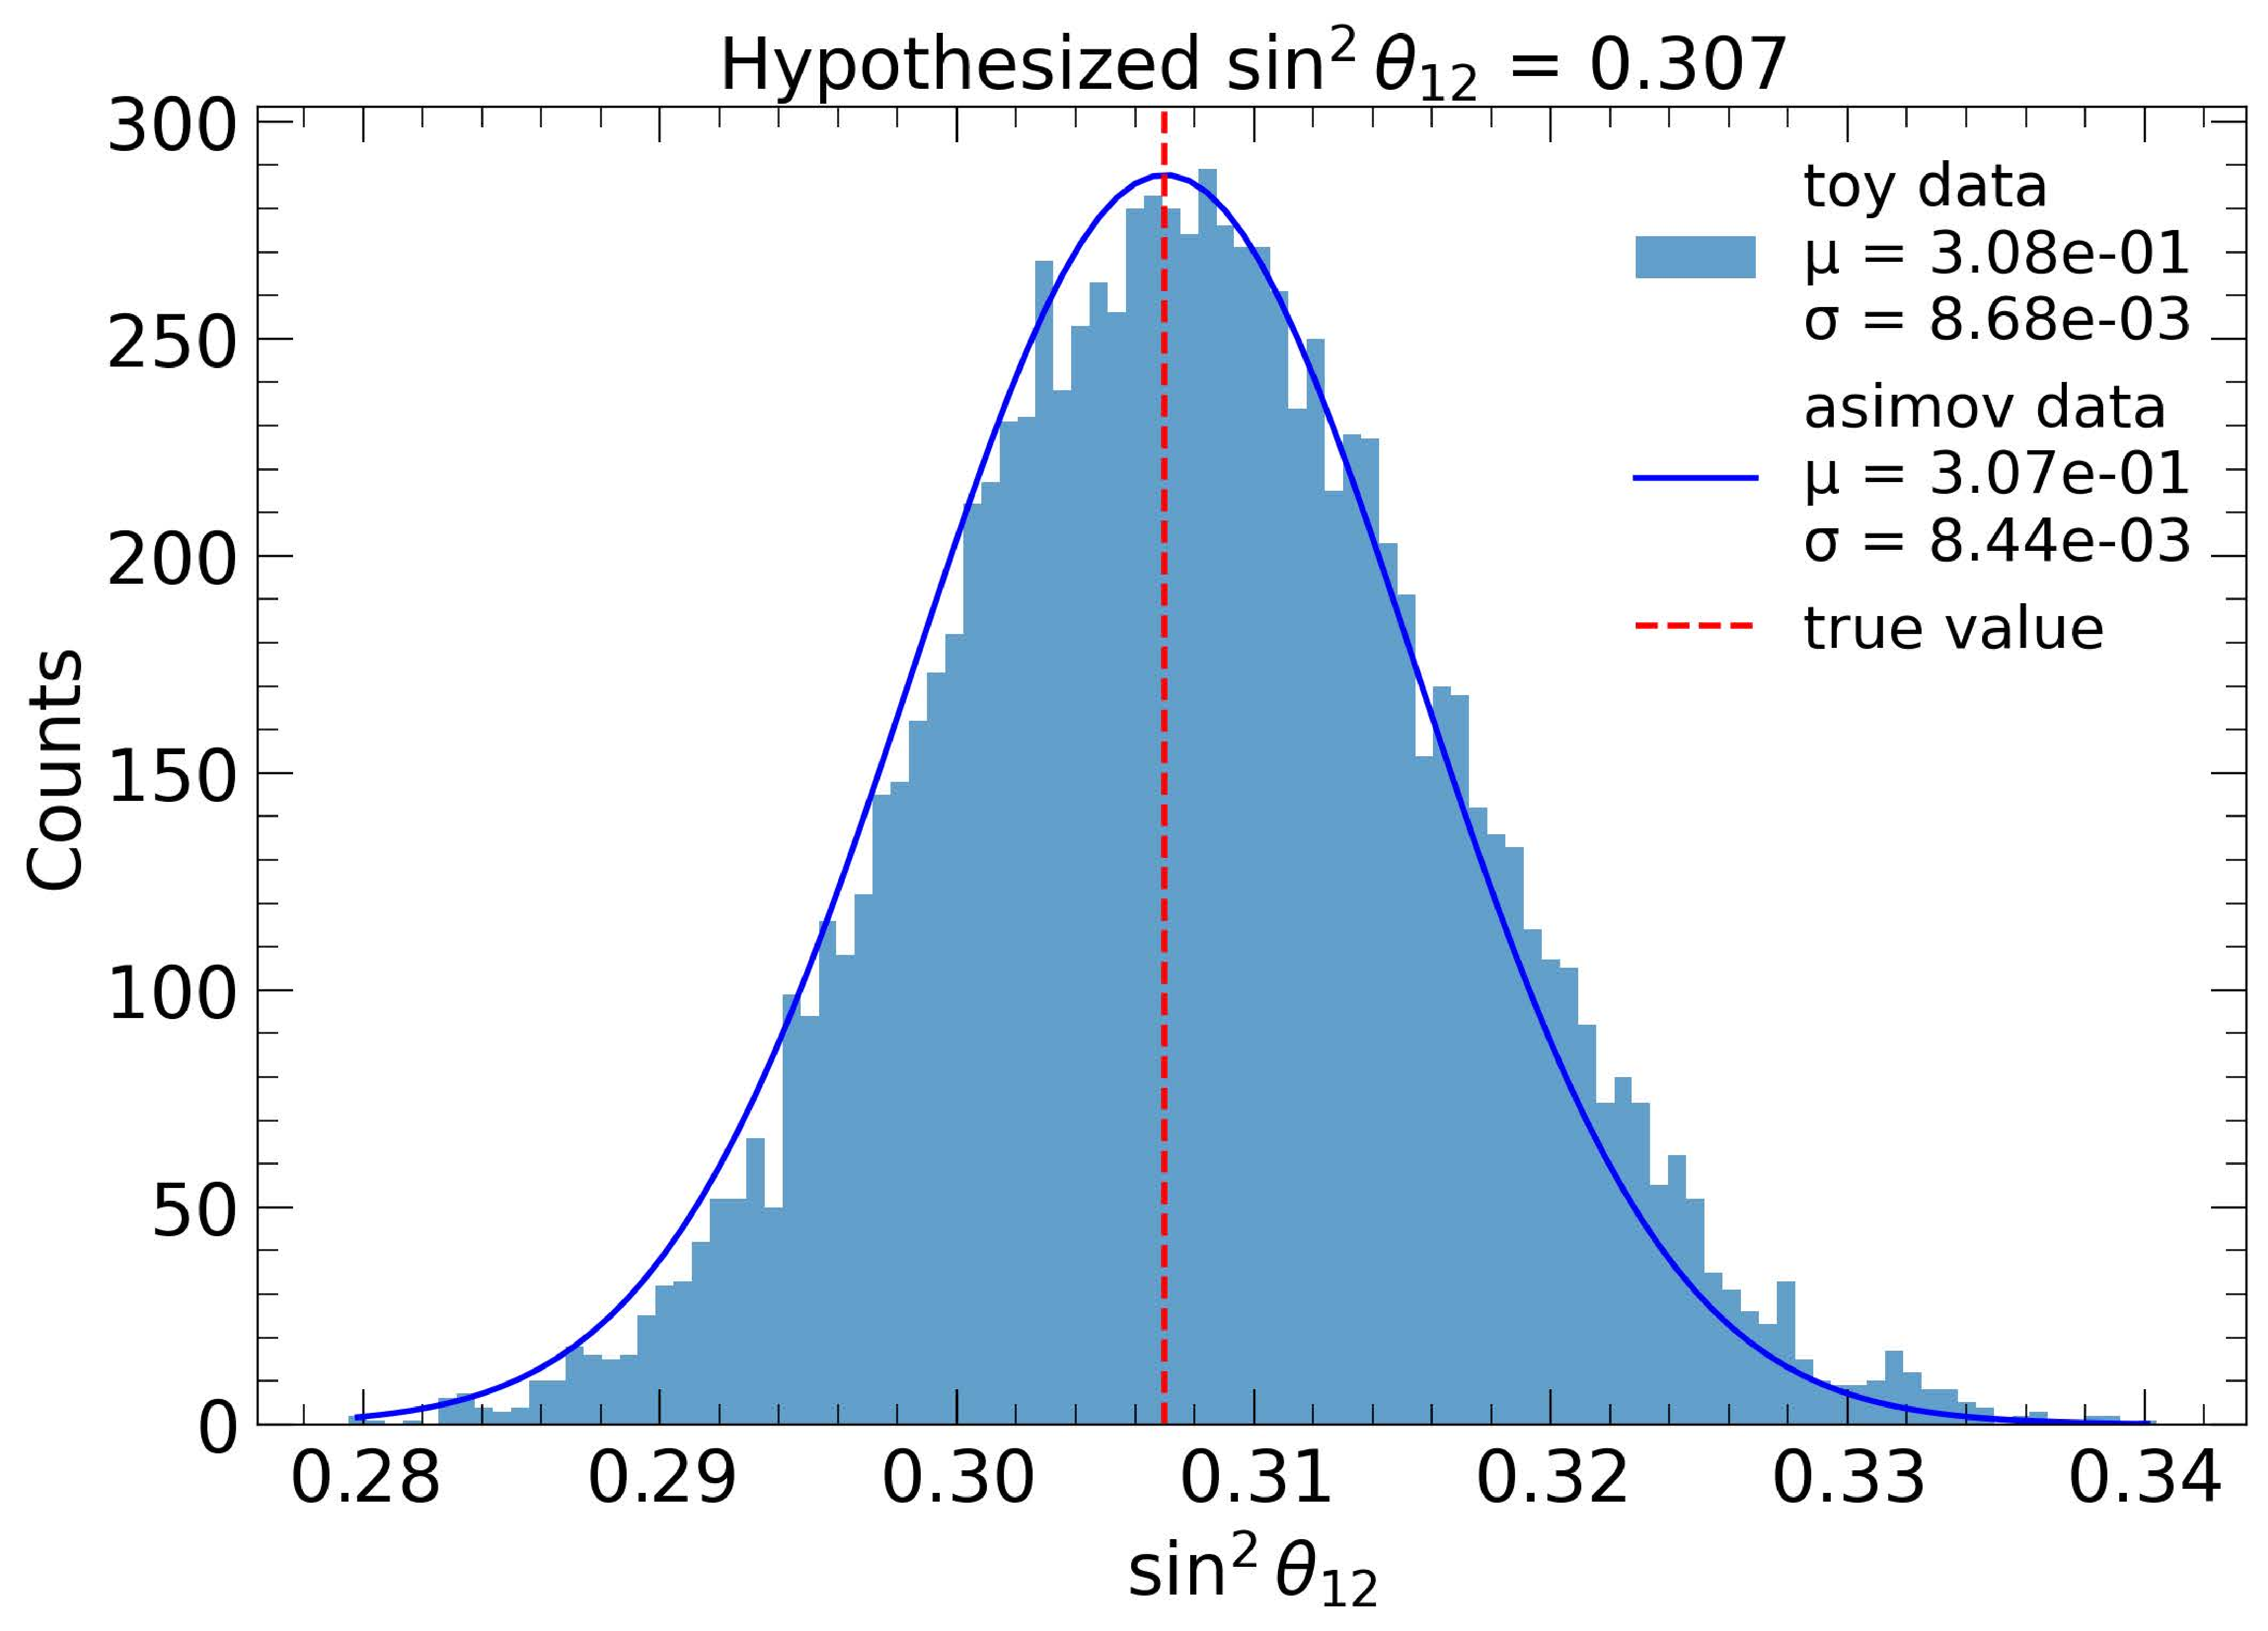
\includegraphics[width=\linewidth]{figs/Section2/Jingqin_sinsq12_bias_56bins.pdf}
    \caption{56 bins.}
    \label{fig:s12_binning_factor10}
  \end{subfigure}
  \caption{Distribution of $\sin \theta_{12}$ best-fit values from 10,000 pseudoexperiments at 30 days exposure and with a different number of bins.}
  \label{fig:s12_binning}
\end{figure}

\autoref{fig:solar_low_stat_bias_bins} shows the evolution of bias as a function of the rebin factor (assuming 560 as the nominal configuration). \autoref{fig:dm2_21_bias_bins} demonstrates that $\Delta m^2_{21}$ at 30 days exposure is largely unbiased, and there is no dependence on the rebin factor. On the other hand, \autoref{fig:s12_bias_bins} shows that $\sin^2\theta_{12}$ exhibits a strong dependence on the binning strategy, with bias decreasing significantly as the rebin factor increases (fewer bins). The bias drops from approximately 0.8$\sigma$ at rebin factor 1 (560 bins) to less than 0.2$\sigma$ at rebin factor 10 (56 bins).

\begin{figure}[h!]
  \centering
  \begin{subfigure}[t]{0.47\textwidth}
    \centering
    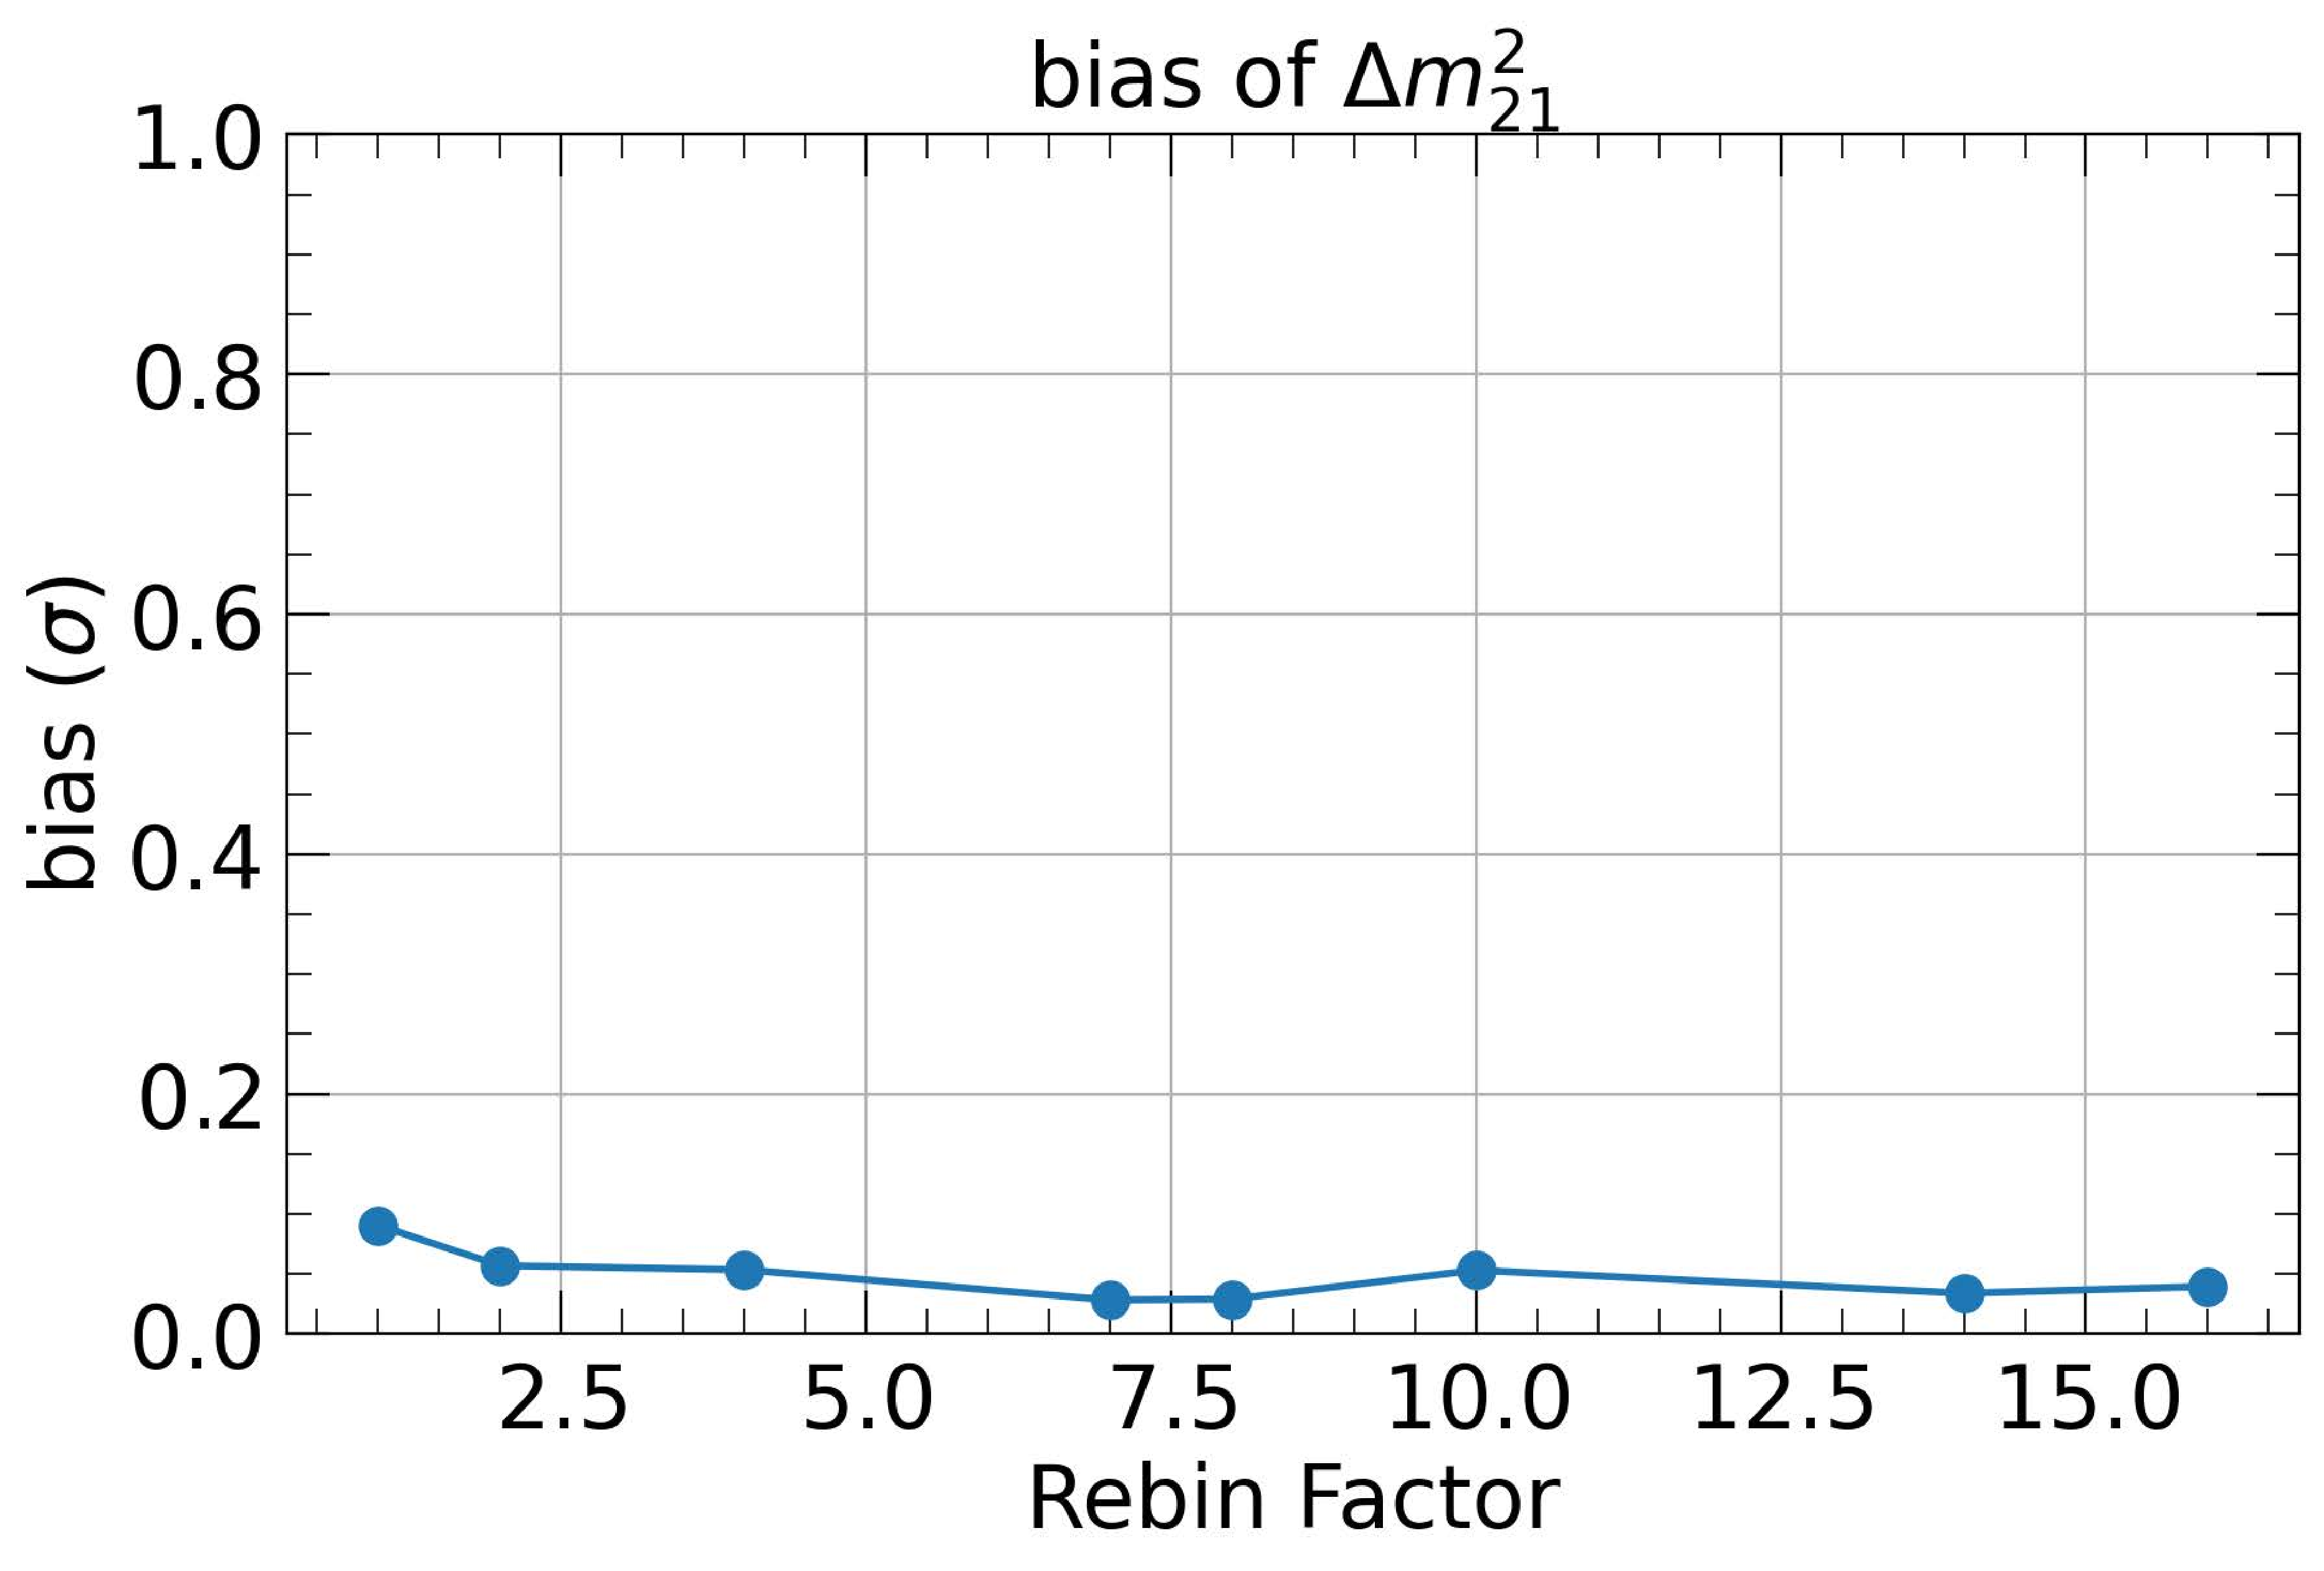
\includegraphics[width=\linewidth]{figs/Section2/Jingqin_dmsq21_bias_dif_bins.pdf}
    \caption{$\Delta m^2_{21}$ bias as a function of the rebin factor.}
    \label{fig:dm2_21_bias_bins}
  \end{subfigure}
  \hfill
  \begin{subfigure}[t]{0.47\textwidth}
    \centering
    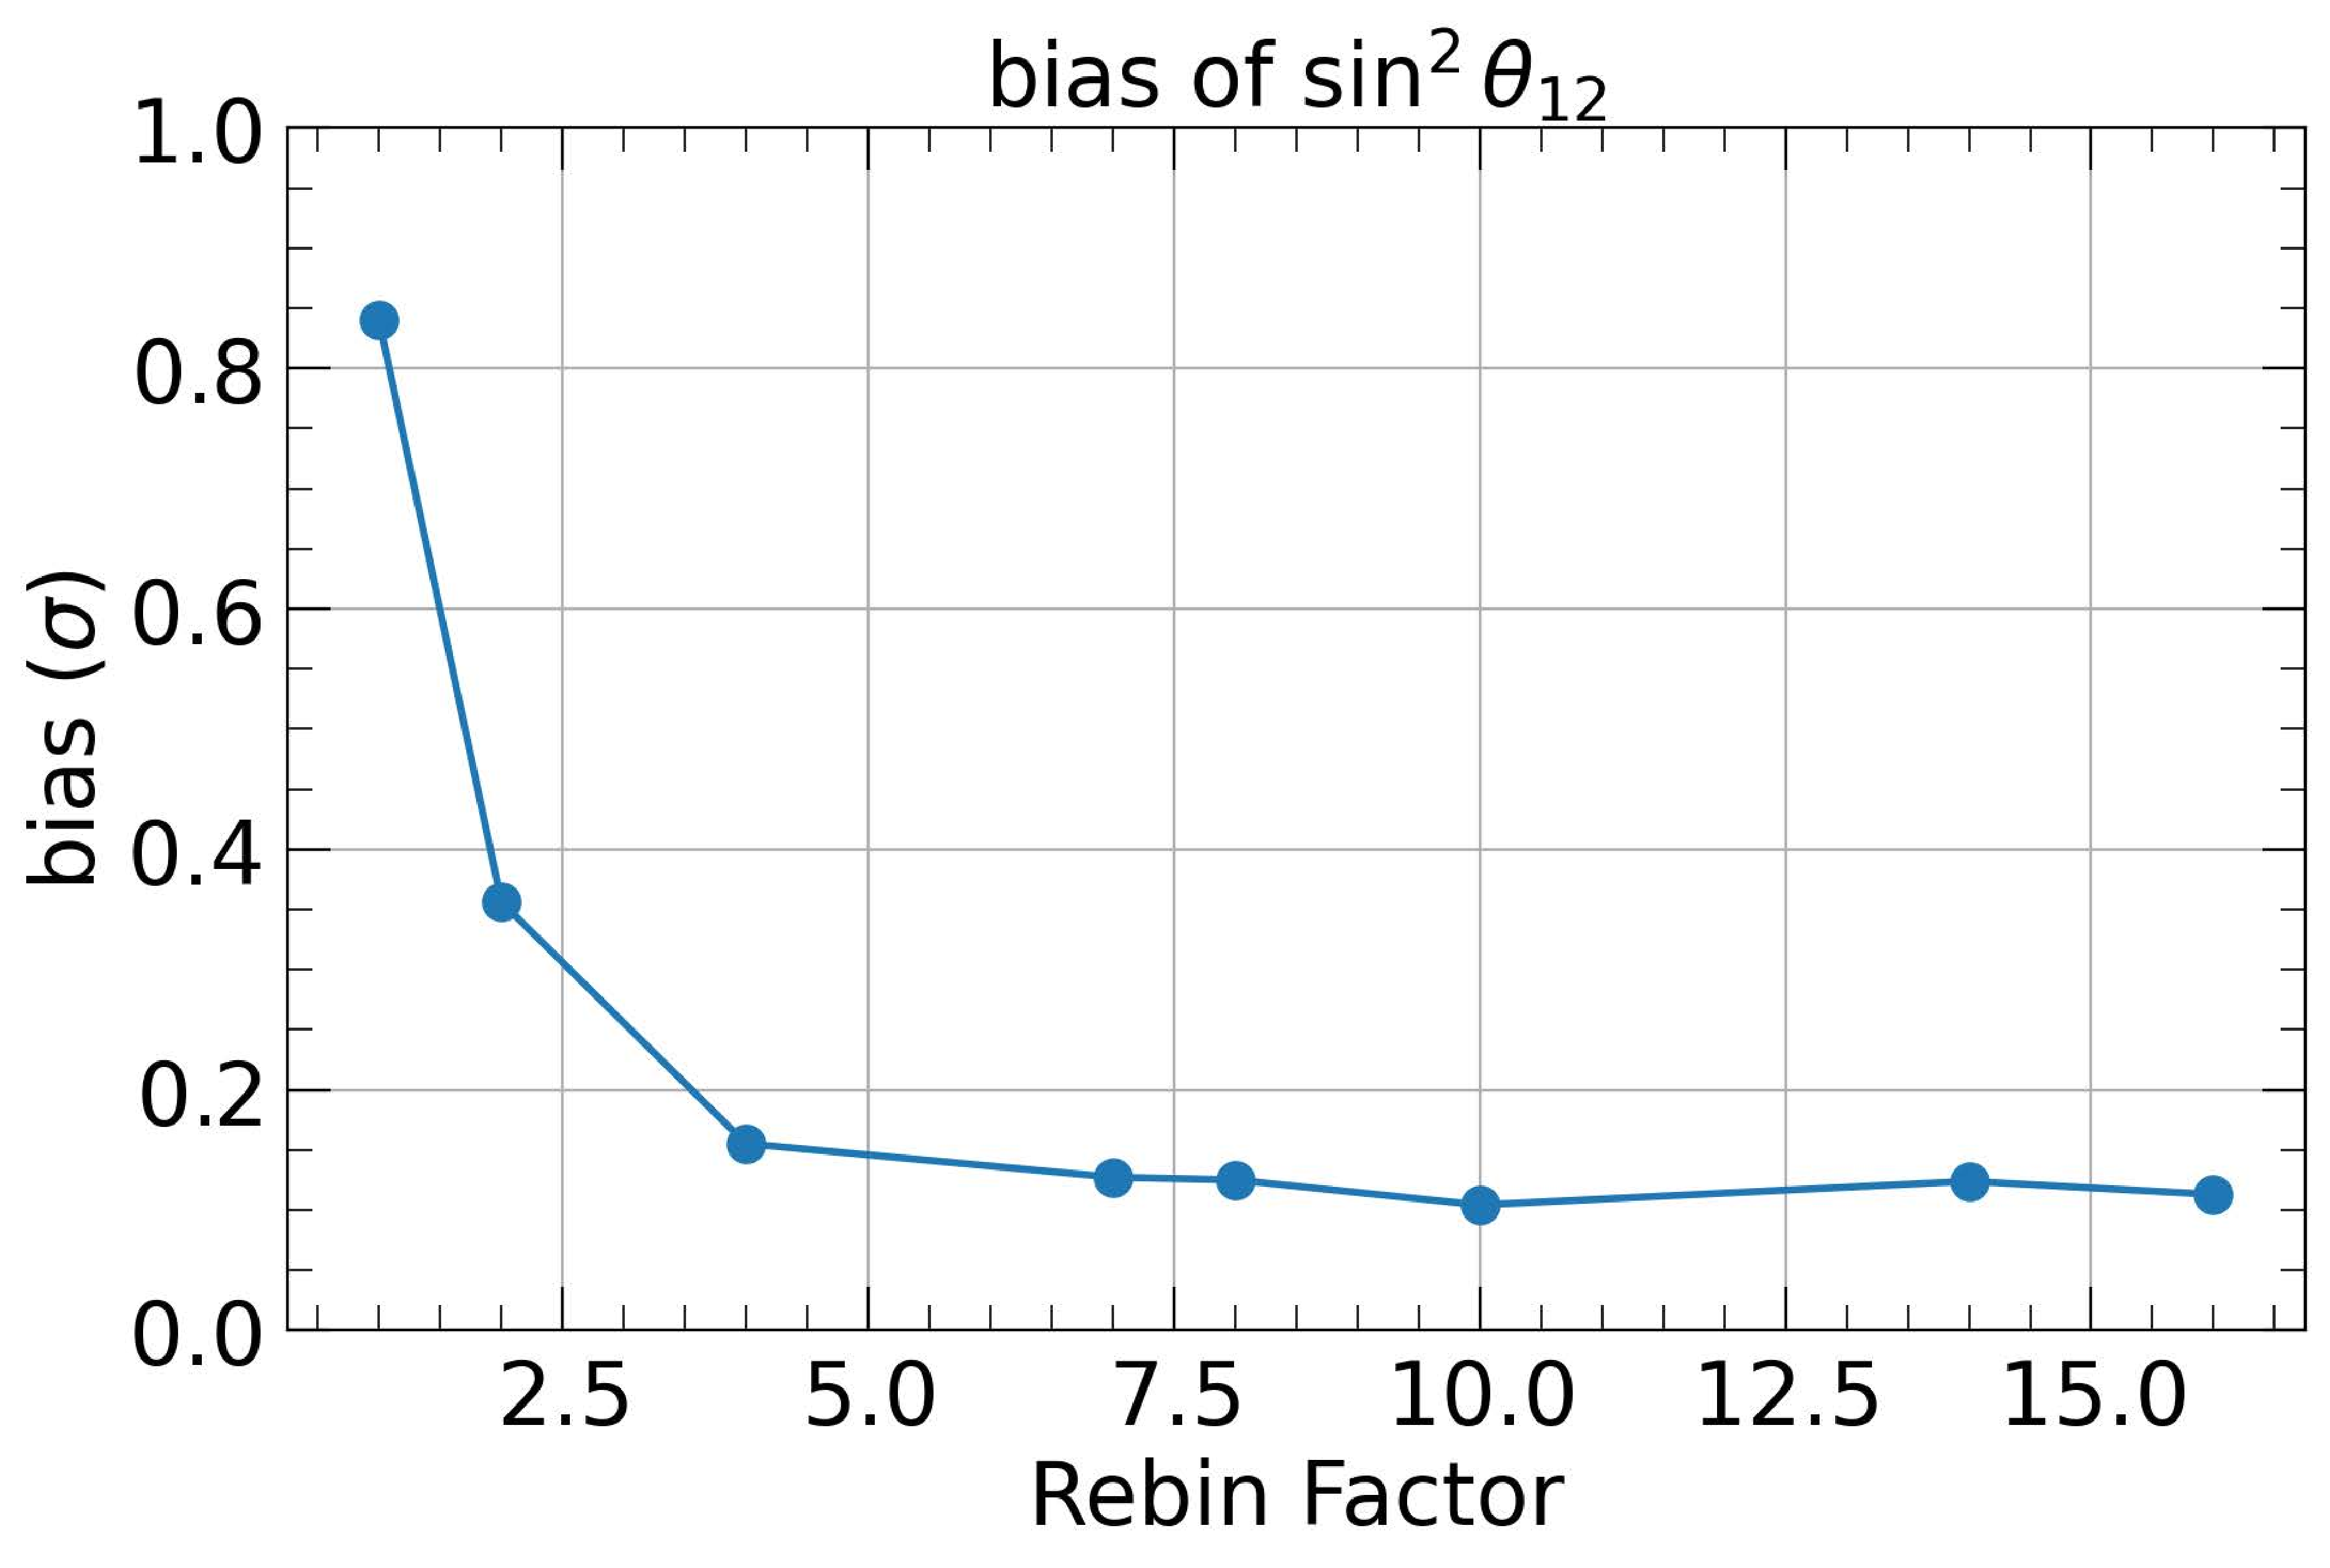
\includegraphics[width=\linewidth]{figs/Section2/Jingqin_sinsq12_bias_dif_bins.pdf}
    \caption{$\sin^2\theta_{12}$ bias as a function of the rebin factor.}
    \label{fig:s12_bias_bins}
  \end{subfigure}
  \caption{Evolution of bias of solar oscillation parameters as function of the rebin factor.}
  \label{fig:solar_low_stat_bias_bins}
\end{figure}



% \subsubsection{Feldman-Cousin test for $\Delta m^2_{21}$}
% {\color{red} Yes or no?}

\subsection{Conclusions of this Section}
The measurement of solar parameters does not appear to pose significant challenges, with both $\Delta m^2_{21}$ and $\sin^2\theta_{12}$ exhibiting well-behaved statistical properties at low exposure. The main results are:
\begin{itemize}
    \item $\Delta m^2_{21}$ shows very small bias (less than 0.1$\sigma$) at all exposure levels and remains unaffected by different binning choices.
    \item $\sin^2\theta_{12}$ shows some bias at very short exposures (30 days), but this can be easily controlled by using fewer, larger energy bins.
    \item With the nominal configuration under study, JUNO can achieve better precision than current global results within the first month of data taking. 
\end{itemize}
Therefore, as long as systematic uncertainties are well controlled through proper detector calibration and background modeling (especially geoneutrinos), JUNO is expected to achieve world-leading measurements of solar oscillation parameters within the first months of operation.


\section{$\Delta m^2_{31}$ Constraints from DYB}\label{sec:dm231constraints}
Studies on JUNO-only $\Delta m^2_{31}$ measurements in \autoref{sec:coverage} have shown that under low statistics, JUNO's measurement of $\Delta m^2_{31}$ is likely to have multiple disjoint intervals and bad minima. A possible mitigation strategy is incorporating an external $\Delta m^2_{31}$ constraint to help exclude the bad minima and reduce the probability of getting disjoint intervals. In this study, we utilize the Daya Bay $\Delta m^2_{31}$ with ~2.3\% precision and assume no correlation between Daya Bay's measured $\Delta m^2_{31}$ and $\rm sin^2\theta_{13}$. The constraint from Daya Bay not only helps JUNO exclude the bad minima to obtain a single interval, but also provides a reactor-only $\Delta m^2_{31}$ measurement for global fit or non-reactor experiments. It is worth noting that besides Daya Bay serving as external constraint, other external constraints with better precision than JUNO's could also be used (e.g. PDG2025). 

\subsection{Statistic and $\Delta m^2_{31}$ pull}
In this section, the statistic is consistently the $\chi^2$ as defined in \autoref{eq:chi_sq}. Similar to implementing external $\rm sin^2\theta_{13}$ constraint, we add an additional pull term, 
\begin{equation}
\chi^2(\Delta m^2_{31}) = \left(\frac{\Delta m^2_{31} - \Delta m^{2,0}_{31}}{\Delta m^{2,0}_{31} \times \sigma(\Delta m^2_{31})}\right)^2
\end{equation}
to constrain $\Delta m^2_{31}$, where the $\sigma(\Delta m^2_{31})$ is the precision of the Daya Bay $\Delta m^2_{31}$ measurement (2.3\%). Since the profile $\Delta\chi^2$ of $\Delta m^2_{31}$ still potentially has local minima under external $\Delta m^2_{31}$ constraint, the Feldman-Cousins method to ensure coverage is necessary. The test statistic remains the likelihood-ratio test statistic $\Delta\chi^2$ as defined in \autoref{eq:lambda_i}. The handling of nuisance parameters and statistical fluctuation in the MC generation is same as described in \autoref{appendix:pseudoexp}. The only noticed is the additional sampling of the central value $\Delta m^{2,0}_{31}$ for the $\Delta m^2_{31}$ pull term. For each JUNO toy MC, a new $\Delta m^{2,0}_{31}$ is sampled from a Gaussian distribution centered at the true $\Delta m^2_{31}$ with a 2.3\% precision, such that each JUNO toy corresponds to a different $\Delta m^{2,0}_{31}$ to simulate different Daya Bay pseudo-experience measurements. The distribution of $\Delta\chi^2$ from fitting all toys is used to correct the critical $\Delta\chi^2_{\rm crit}$ at different confidence levels.

\subsection{FC-based $\Delta m^2_{31}$ sensitivity}
Under low statistics, we took JUNO 50 days and 100 days of data taking time as examples, and scanned 50 uniformly distributed values within the range of $[2, 3] \times 10^{-3}\rm\ eV^2$ as the assumed true $\Delta m^2_{31}$ for hypothesis test. For each combination of data taking time and true $\Delta m^2_{31}$ value, we generate 5000 JUNO toys, which is sufficient to extract the $\Delta\chi^2_{\rm crit}$ corresponding to $1\sigma~(68.27\%)$.
\autoref{fig:juno_dyb_pull_deltachi2_dist} shows the $\Delta\chi^2$ distributions from fit of all toys given one certain true value for 50-days and 100-days data. Compared to the $\chi^2$ distribution with 1 degree of freedom, the $\Delta\chi^2$ distribution has a slightly long tail, leading to a $\Delta\chi^2_{\rm crit}$ for $1\sigma$ slightly larger than 1 expected by Wilks' theorem.
\begin{figure}[h]
  \begin{subfigure}[t]{0.47\textwidth}
    \centering
    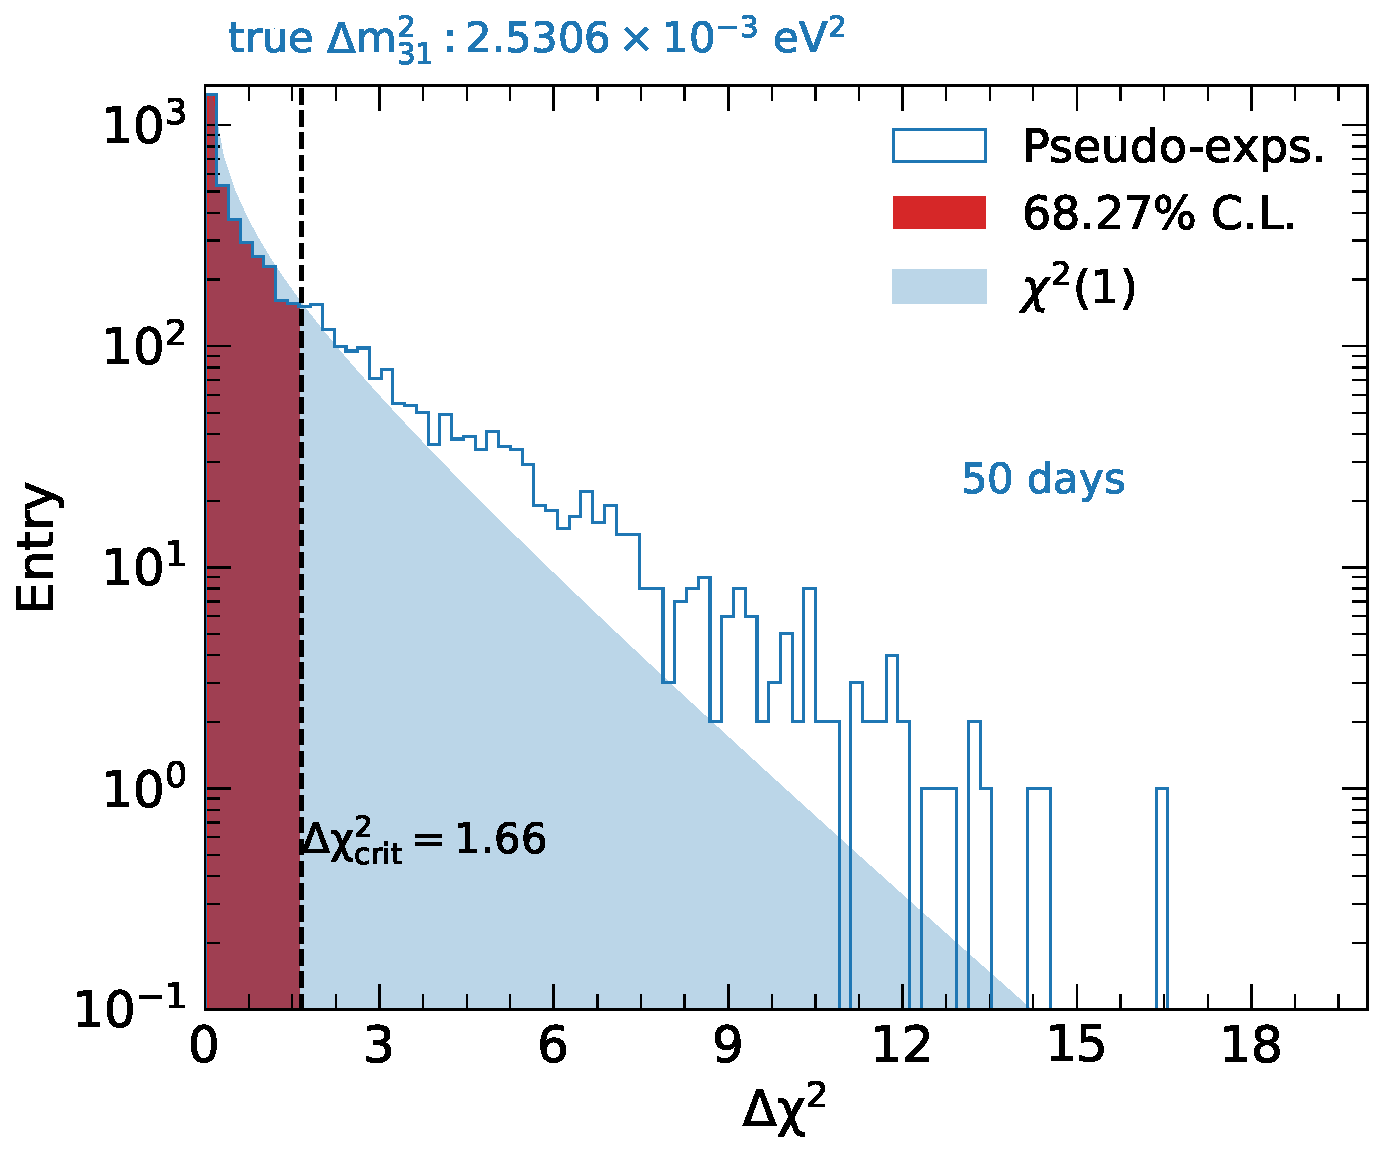
\includegraphics[width=\linewidth]{figs/Section2/han_juno_dybpull_hist_deltachi2_50days_2dpull_logV_correct_subplot.pdf}
    \caption{50 days}
    \label{fig:juno_dyb_pull_50d_deltachi2}
  \end{subfigure}
  \hfill
  \begin{subfigure}[t]{0.47\textwidth}
    \centering
    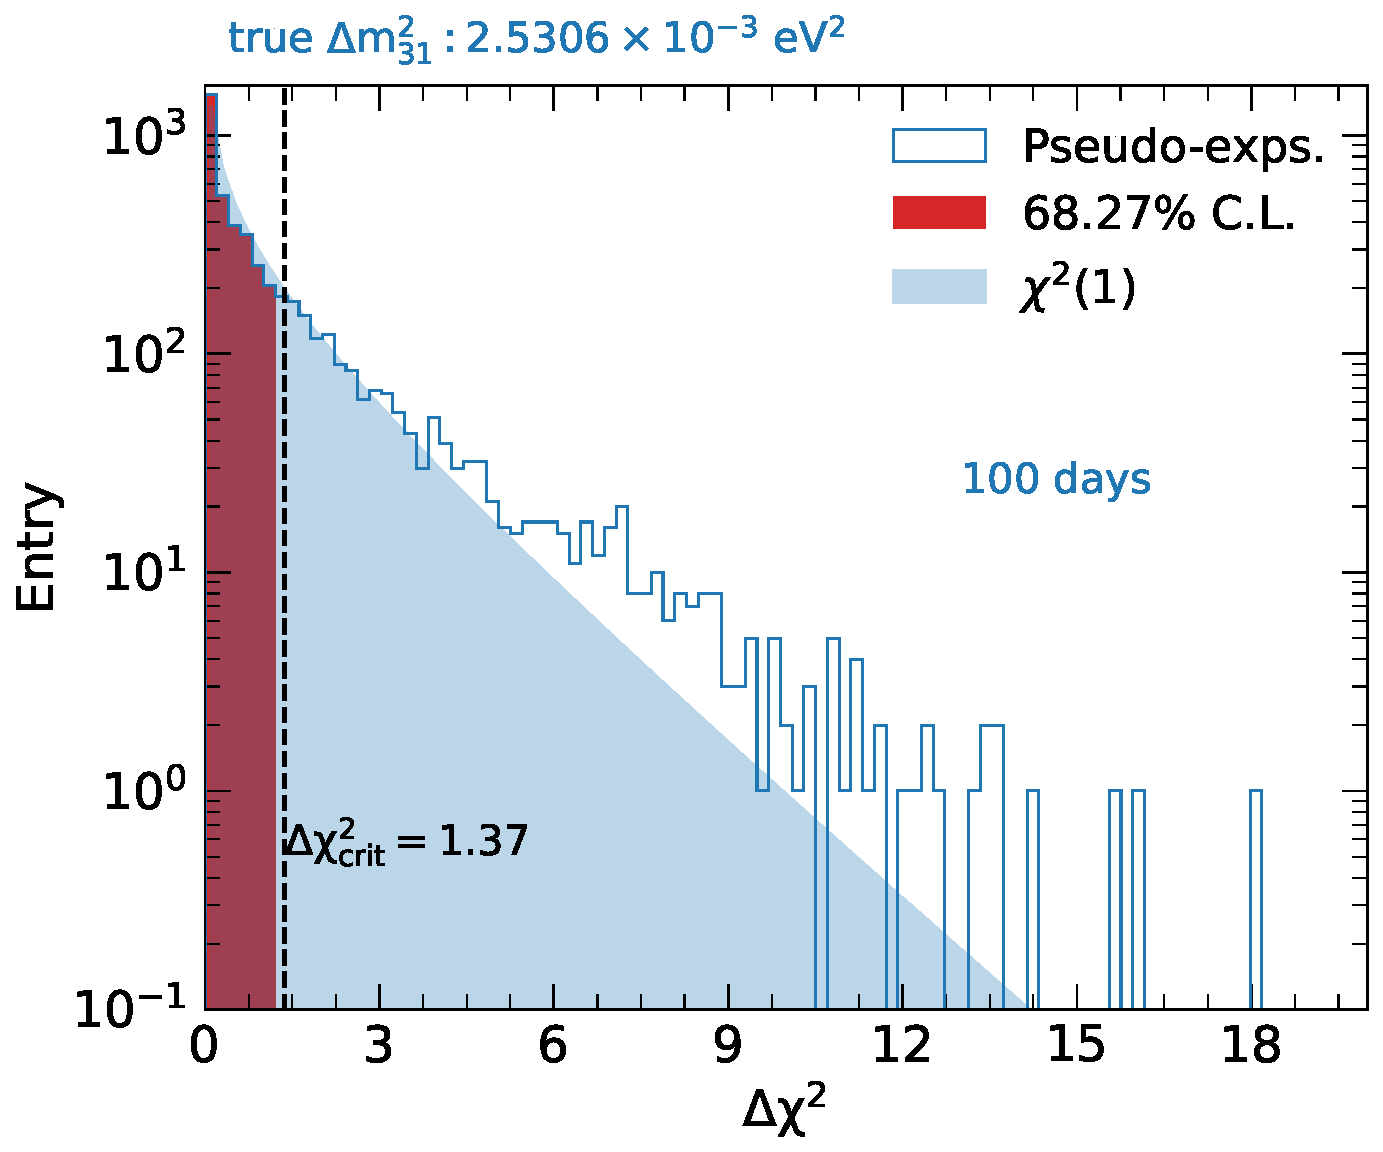
\includegraphics[width=\linewidth]{figs/Section2/han_juno_dybpull_hist_deltachi2_100days_2dpull_logV_correct_subplot.pdf}
    \caption{100 days}
    \label{fig:juno_dyb_pull_100d_deltachi2}
  \end{subfigure}
  \caption{The $\Delta\chi^2$ distribution and the corresponding $\Delta\chi^2_{\rm crit}$, assuming a certain true $\Delta m^2_{31}=2.53\times10^{-3}$ $\rm{eV^2}$.}
  \label{fig:juno_dyb_pull_deltachi2_dist}
\end{figure}
Given a JUNO dataset, $\Delta m^2_{31}$ values satisfying $\Delta\chi^2 < \Delta\chi^2_{\rm crit}$ are included in the confidence interval which may be disjoint islands. To describe the $\Delta m^2_{31}$ sensitivity, we define the precision as $\sigma_{\rm width}/(2\times\Delta m^{2,\rm bft}_{31}$), here $\sigma_{\rm width}$ is the total width of the confidence interval and $\Delta m^{2,\rm bft}_{31}$ is the best-fit value. In order to evaluate the FC-based sensitivity of $\Delta m^2_{31}$, we additionally generate 5000 validation toys and sample the $\Delta m^{2,0}_{31}$ assuming the best-fit $\Delta m^2_{31}$ under normal ordering from the Daya Bay as the true value. \autoref{fig:juno_dyb_pull_toy_example} illustrates a validation toy example. Statistical fluctuation induced fluctuation in the critical line (orange dashed line); after smoothing, $\Delta\chi^2_{\rm crit}$ slightly depends on the true $\Delta m^2_{31}$ value. The green solid line is the profiled $\Delta\chi^2$ of $\Delta m^2_{31}$ under the $\Delta m^2_{31}$ constraint, and the $1\sigma$ confidence interval (blue span) is obtained using the corrected $\Delta\chi^2_{\rm crit}$.
\begin{figure}[h]
    \centering
    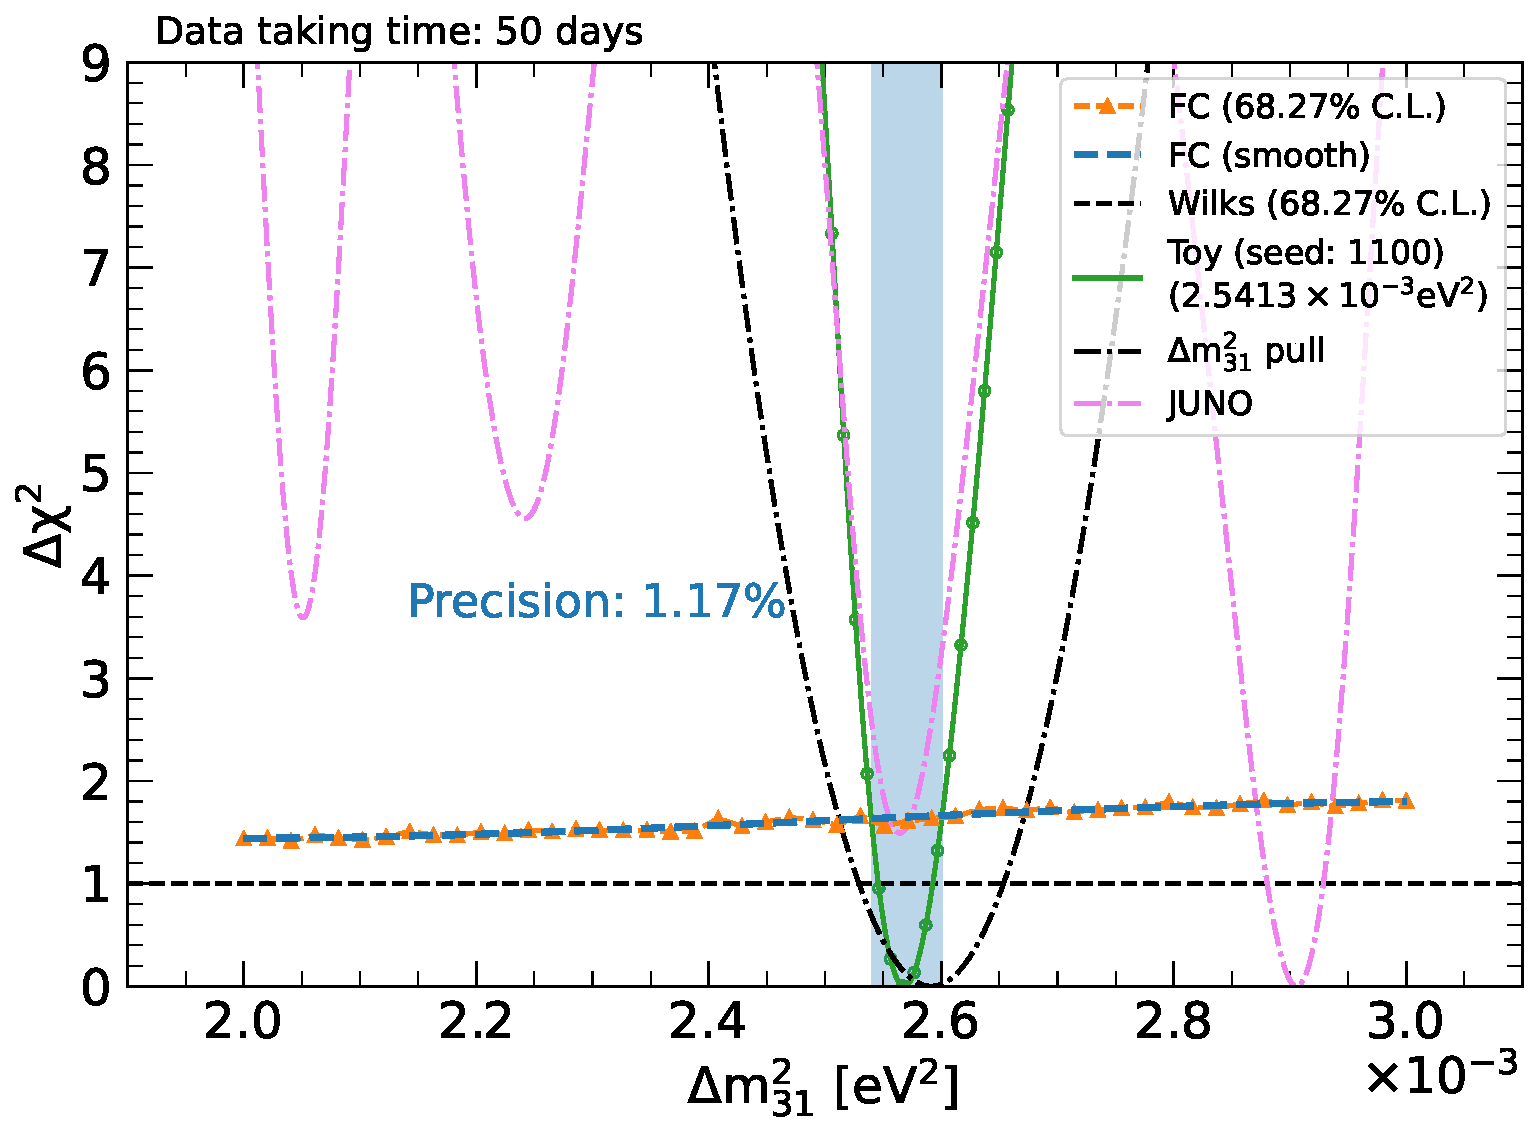
\includegraphics[width=0.6\linewidth]{figs/Section2/han_juno_dybpull_profile_example.pdf}
    \caption{A toy example of precision estimation using the corrected $\Delta\chi^2_{\rm crit}$}
    \label{fig:juno_dyb_pull_toy_example}
\end{figure}
It's obvious that the interval width is larger than that given by Wilks' theorem. With the best-fit value and confidence interval, the $\Delta m^2_{31}$ precision for this toy experiment is easily estimated. As shown in the left panel of \autoref{fig:juno_dyb_pull_num_pre_50d} for 50 days of data-taking, after estimating the confidence intervals for 5000 validation toys, we found that only a small fraction (9.7\%) of toys have $1\sigma$ confidence interval composed of two disjoint islands, while most toys, as expected, have a single interval with other bad minima excluded. The right panel of \autoref{fig:juno_dyb_pull_num_pre_50d} shows the distribution of $\Delta m^2_{31}$ precision and the median precision is used to describe the FC-based $\Delta m^2_{31}$ sensitivity. Compared with \autoref{fig:juno_dyb_pull_num_pre_100d} for 100 days of data-taking, the probability of obtaining disjoint islands decreases to 5.6\%.
\begin{figure}[h]
    \centering
    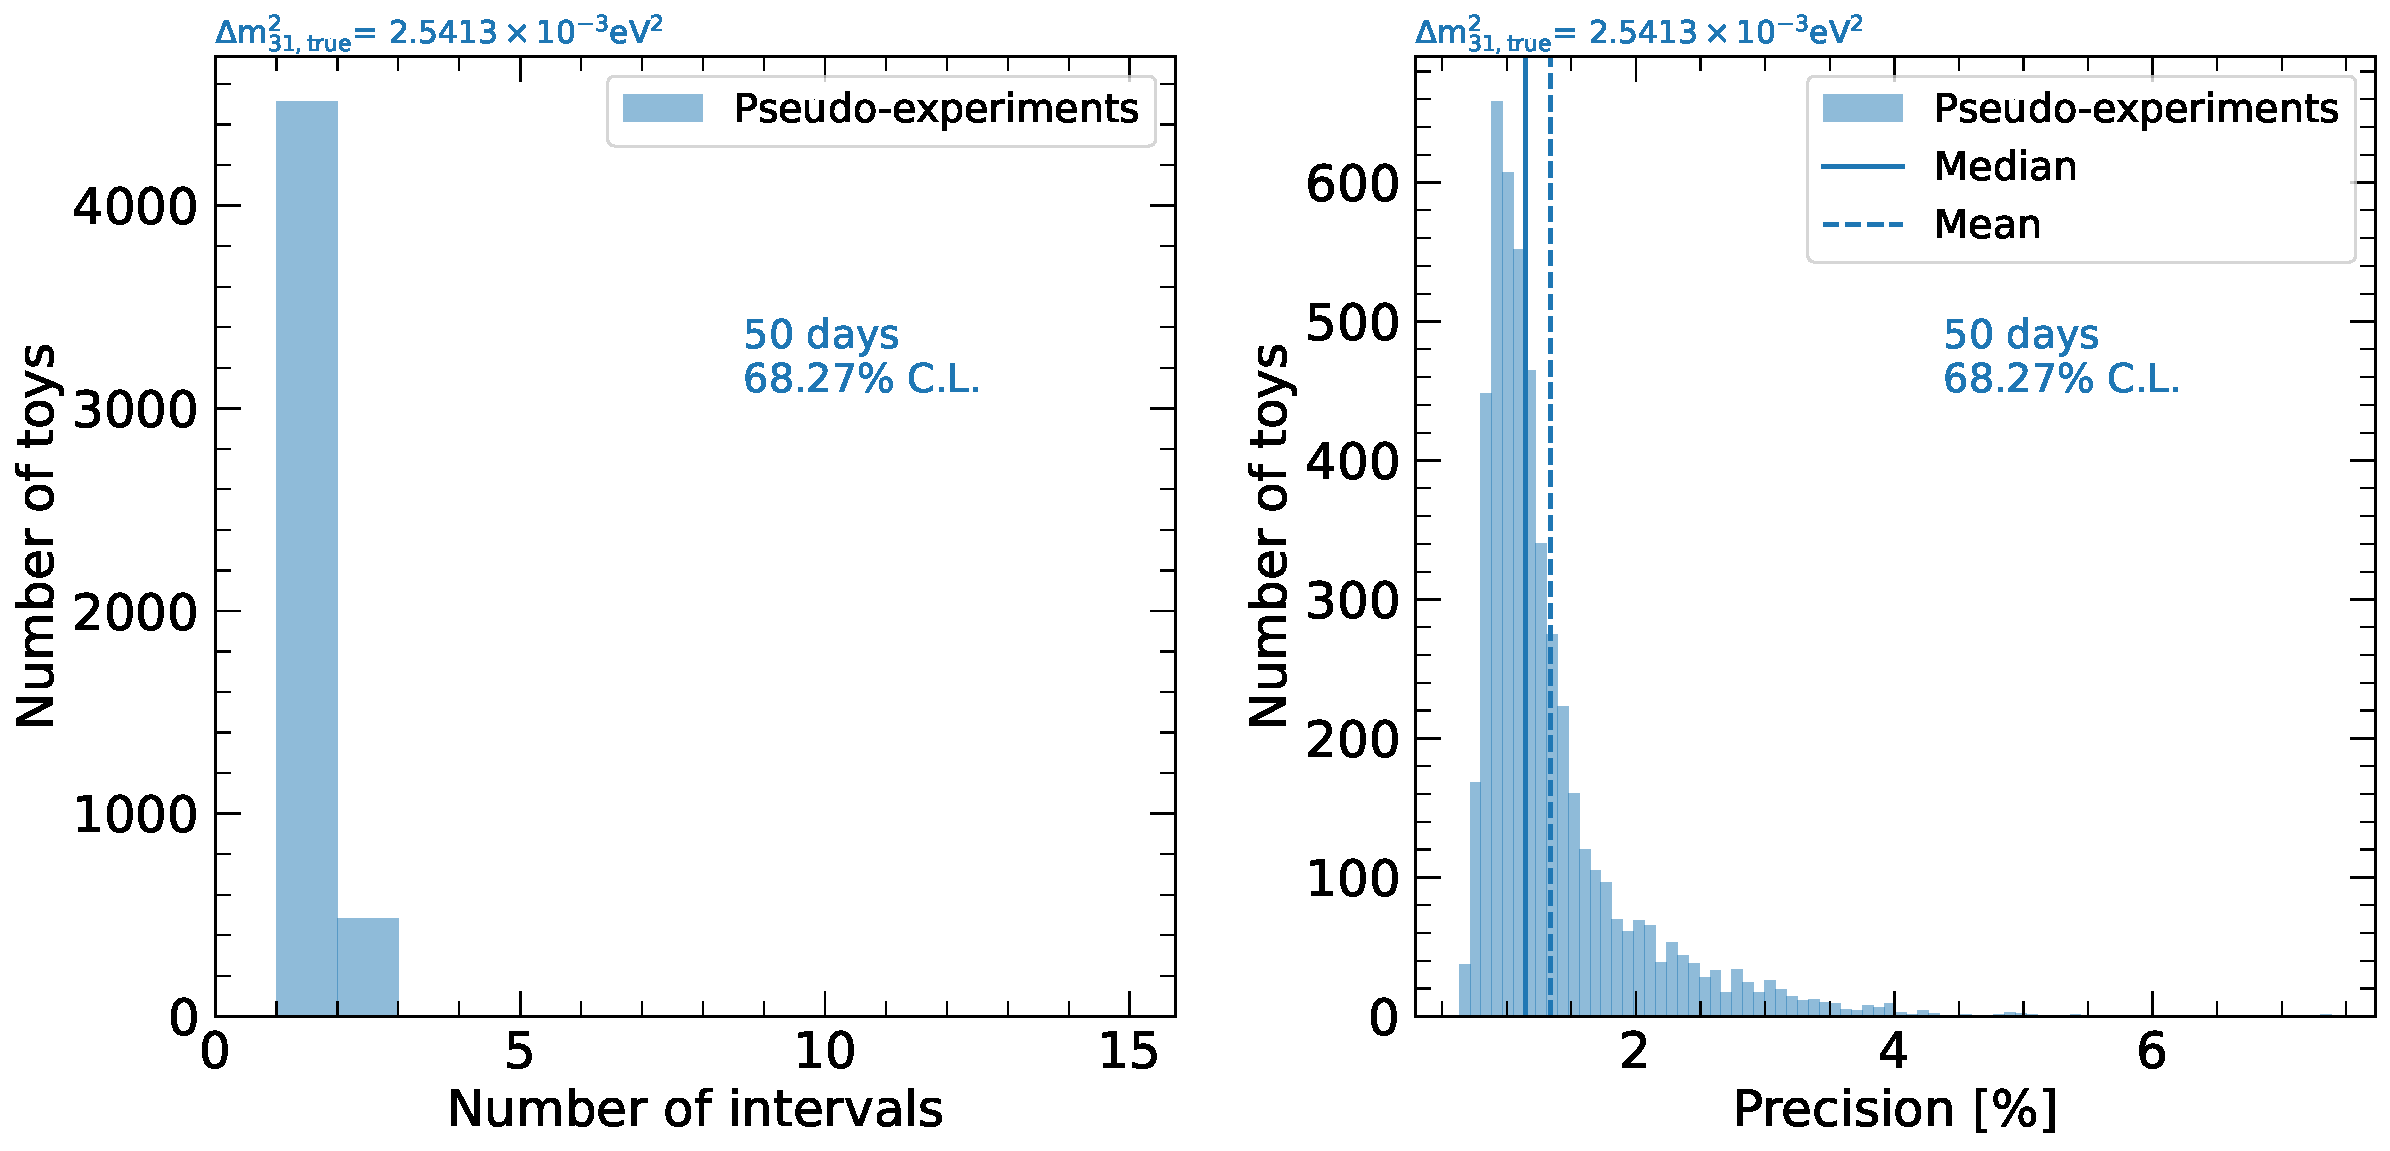
\includegraphics[width=0.8\linewidth]{figs/Section2/han_juno_dybpull_num_intervals_precision_50day.pdf}
    \caption{Distribution of the number of disjoint intervals for 68.27\% confidence level, and the distribution of the precision for 50 days of data-taking time. True $\Delta m^2_{31}$ is taken as Daya Bay measurement.}
    \label{fig:juno_dyb_pull_num_pre_50d}
\end{figure}
\begin{figure}[h]
    \centering
    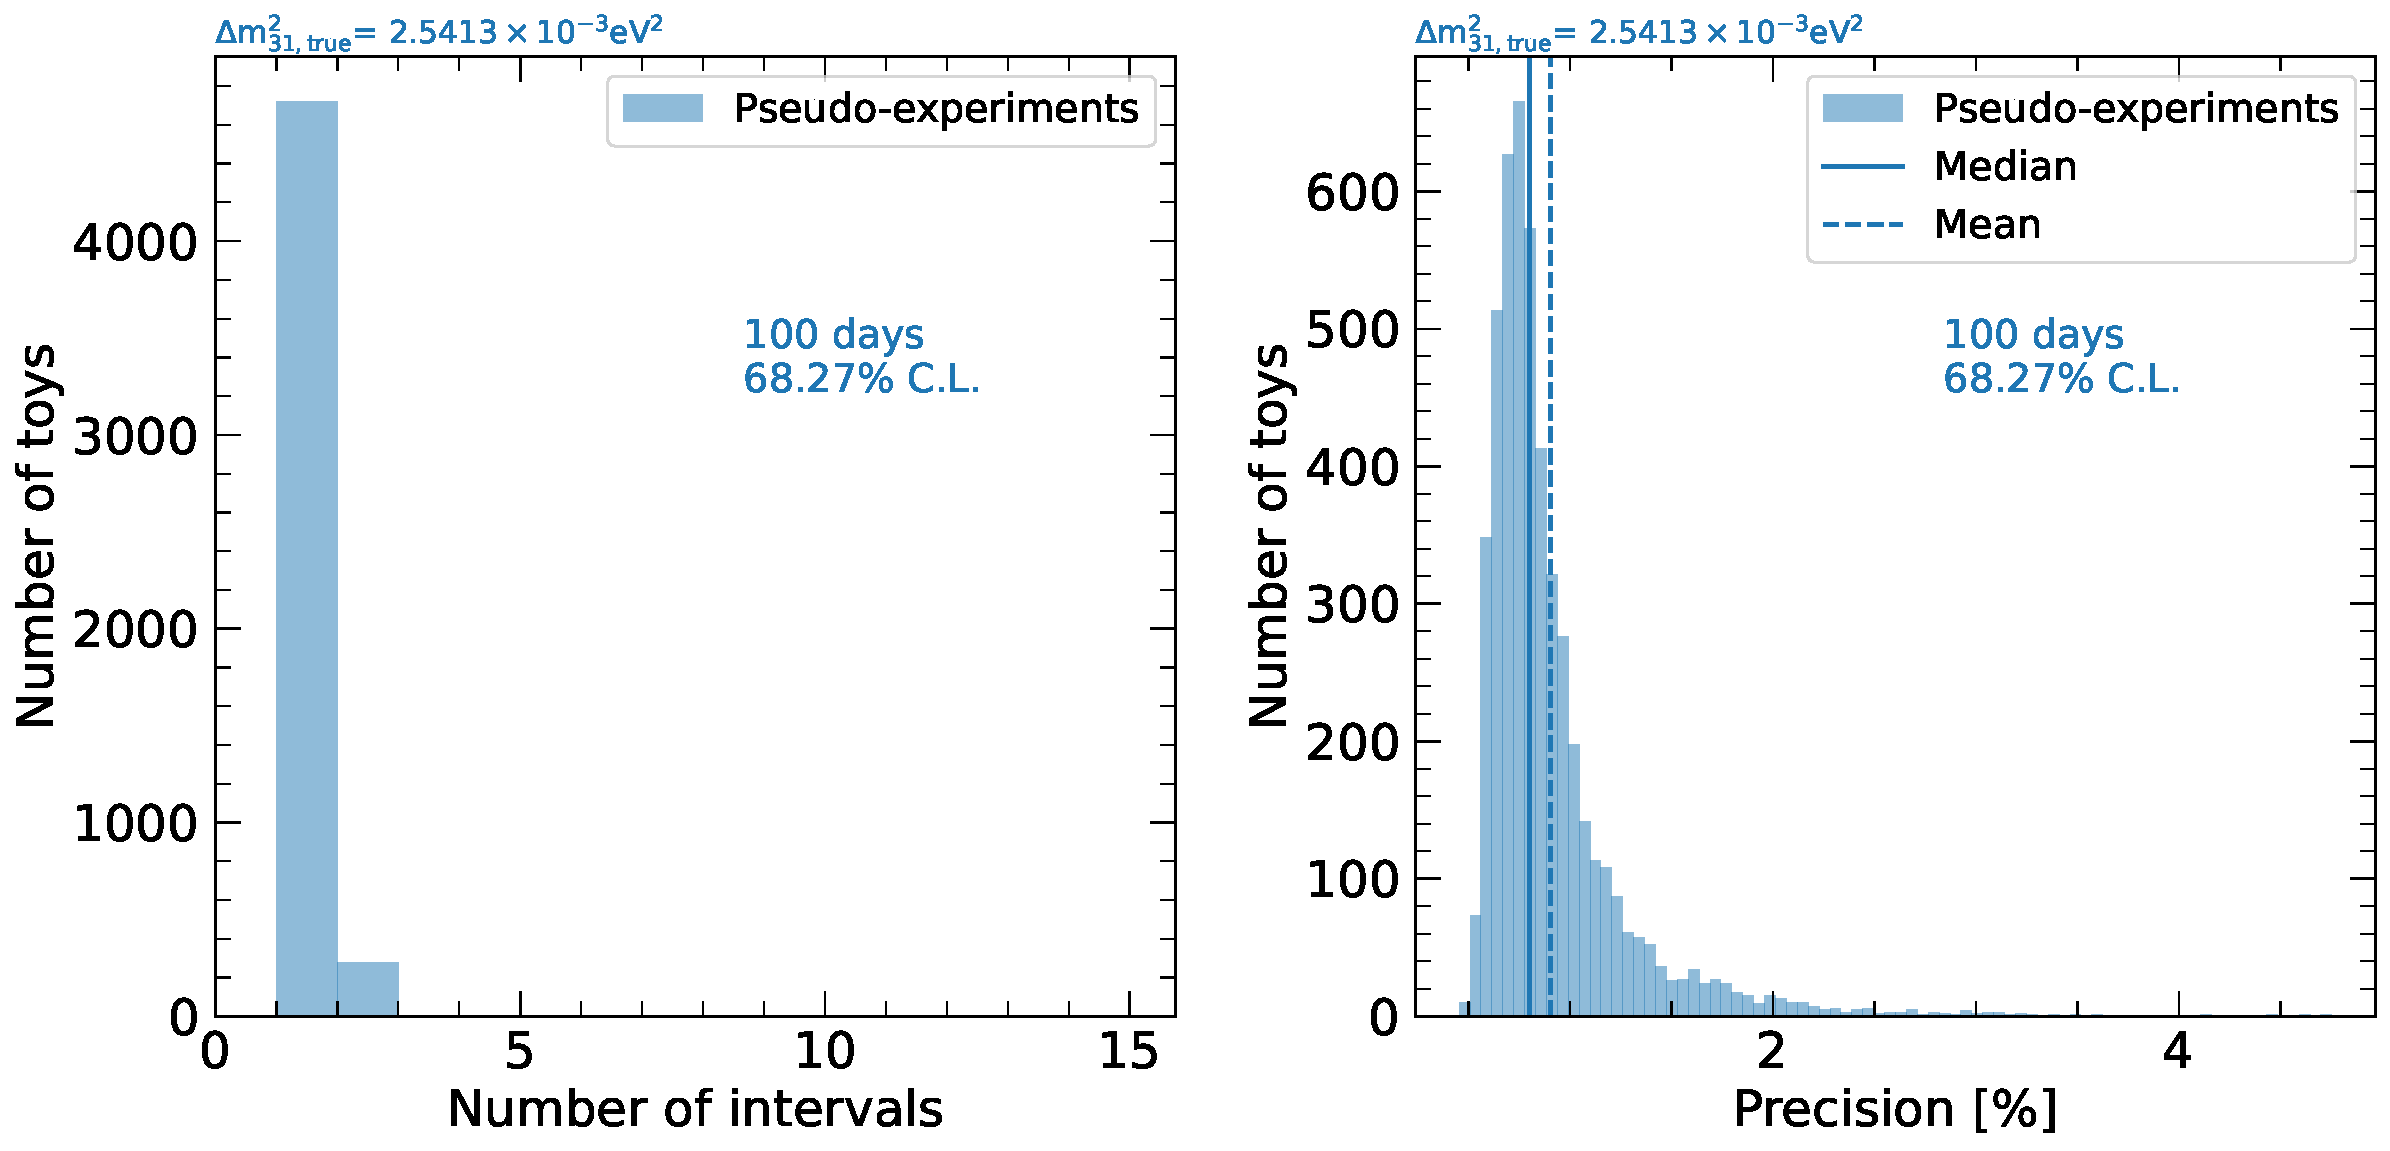
\includegraphics[width=0.8\linewidth]{figs/Section2/han_juno_dybpull_num_intervals_precision_100day.pdf}
    \caption{Distribution of the number of disjoint intervals for 68.27\% confidence level, and the distribution of the precision for 100 days of data-taking time. True $\Delta m^2_{31}$ is taken as Daya Bay measurement.}
    \label{fig:juno_dyb_pull_num_pre_100d}
\end{figure}
The $\Delta m^2_{31}$ sensitivity is 1.14\% for 50-days JUNO statistics which is comparable with global fit, and 0.80\% for 100-days statistics. It should be noted that the sensitivity value is consistent with the results of previous studies on precision measurements. However, poor precision is still possible due to the long tail in the distribution. As shown in \autoref{fig:juno_dyb_pull_poor_pre_toy}, the toys with poor precision are characterized by the fact that even under the $\Delta m^2_{31}$ constraint, the profile is not quadratic, leading to wide or disjoint confidence intervals. 
% (Put the figure of 100-day data case in the appendix?)

\begin{figure}[h]
  \centering
  \begin{subfigure}[t]{0.47\textwidth}
    \centering
    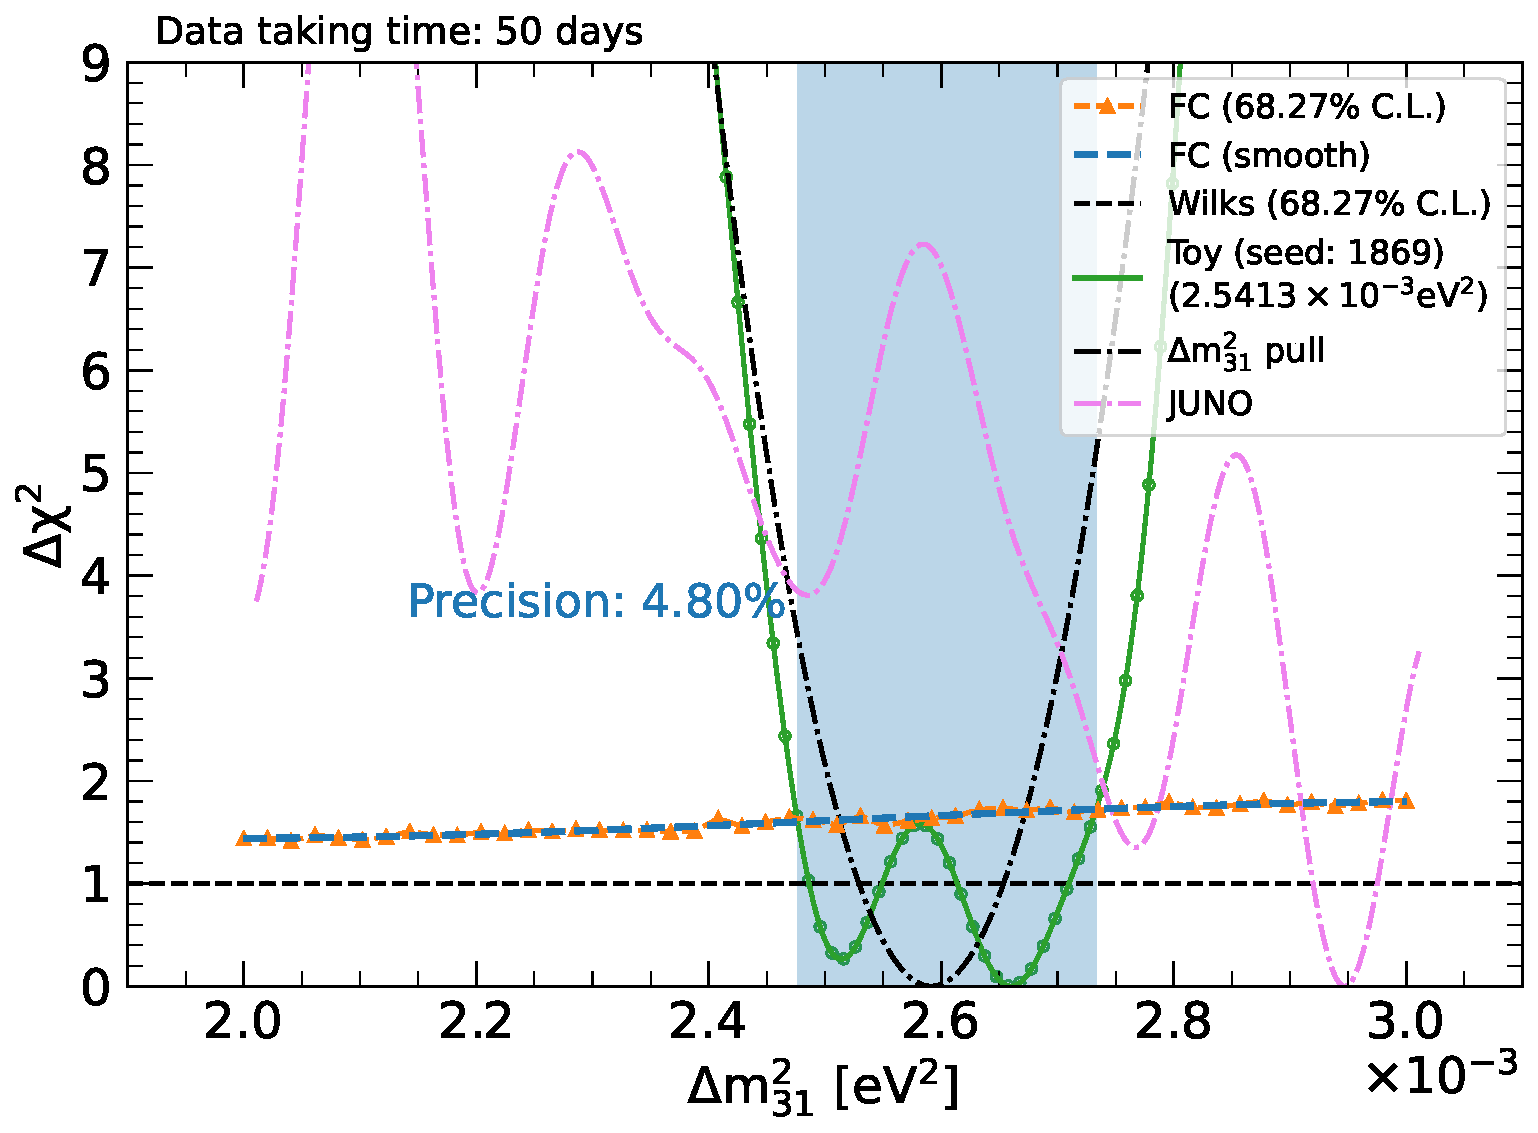
\includegraphics[width=\linewidth]{figs/Section2/han_juno_dybpull_profile_example_poor_pre_1.pdf}
    \caption{}
    \label{fig:l1}
  \end{subfigure}
  \hfill
  \begin{subfigure}[t]{0.47\textwidth}
    \centering
    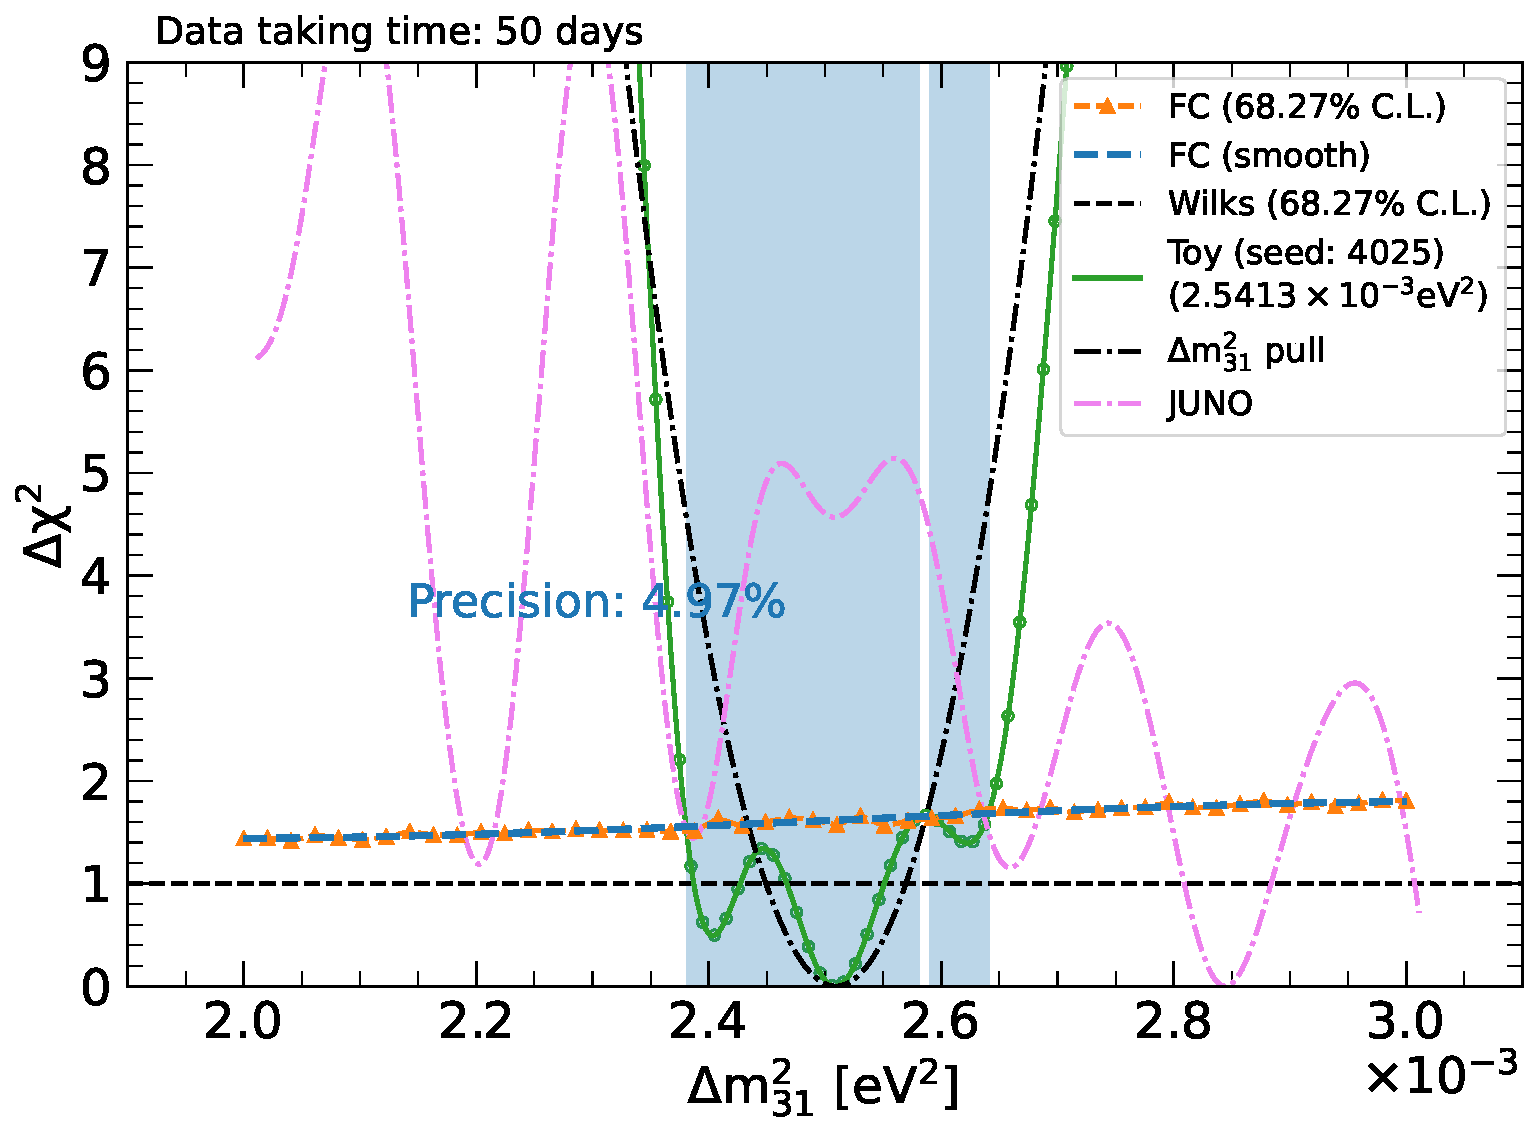
\includegraphics[width=\linewidth]{figs/Section2/han_juno_dybpull_profile_example_poor_pre_2.pdf}
    \caption{}
    \label{fig:l2}
  \end{subfigure}
  \caption{Exceptional toy samples exhibiting poor precision.}
  \label{fig:juno_dyb_pull_poor_pre_toy}
\end{figure}

% \begin{itemize}
%     \item Figure A: distribution of $\Delta\chi^2$ and the corresponding $\Delta\chi^2_{\rm crit}$ for different true $\Delta m^2_{31}$

%     \item Figure B: a toy example of precision estimation using the corrected $\Delta\chi^2_{\rm crit}$

%     \item Figure C: distribution of the number of islands for $1\sigma$ confidence interval, and distribution of the precision

%     \item Figure D: exceptional toy samples exhibiting poor precision.
% \end{itemize}

\subsection{Impact of true $\Delta m^2_{31}$ variation}
In the sensitivity study described in 2.4.2, we not only generate JUNO validation toys to simulate fluctuation in JUNO data but also sample $\Delta m^{2,0}_{31}$ to simulate fluctuations in Daya Bay data. However, in real data analysis, the Daya Bay $\Delta m^2_{31}$ measurement is a fixed result, and the only consideration is how JUNO data fluctuates. Since the true value of $\Delta m^2_{31}$ is unknown, we chose three true values ($\Delta m^{2,\rm{DYB}}_{31}$, $\Delta m^{2,\rm{DYB}}_{31} \pm 3\sigma(\Delta m^{2,\rm{DYB}}_{31})$) to investigate the impact of the true value on $\Delta m^2_{31}$ measurement under Daya Bay constraint. Taking 50-days and 100-days data as examples, 5000 JUNO toys are generated for each true value, and $\Delta m^{2,0}_{31}$ is fixed at the Daya Bay measurement for different toys. Using the profiled $\Delta\chi^2$ from fit and the previously corrected $\Delta\chi^2_{\text{\rm crit}}$, we easily derives the $\Delta m^2_{31}$ precision for each toy. \autoref{tab:frac_interval_pre_50d} and \autoref{tab:frac_interval_pre_100d} show that as the true value deviates from the Daya Bay measurement, the probability of obtaining disjoint confidence intervals increases, and the median precision is worsen.
\begin{table}[!ht]
    \centering
    \begin{tabular}{c|cc|c}
    \toprule
      $\Delta m^2_{31,\rm{true}}$ & Single & Multiple & Median precision \\
    \midrule
      DYB & 96.7\% & 3.3\% & 1.11\% \\
      DYB-3$\sigma$ & 84.0\% & 16.0\% & 1.27\% \\
      DYB+3$\sigma$ & 84.6\% & 15.4\% & 1.29\% \\
    \bottomrule
    \end{tabular}
    \caption{The fraction of toys where have single interval or multiple intervals, and the median precision for 50-days data.}
    \label{tab:frac_interval_pre_50d}
\end{table}

\begin{table}[!ht]
    \centering
    \begin{tabular}{c|cc|c}
    \toprule
      $\Delta m^2_{31,\rm{true}}$ & Single & Multiple & Median precision \\
    \midrule
      DYB & 98.6\% & 1.4\% & 0.79\% \\
      DYB-3$\sigma$ & 81.5\% & 18.5\% & 0.94\% \\
      DYB+3$\sigma$ & 83.1\% & 16.9\% & 0.94\% \\
    \bottomrule
    \end{tabular}
    \caption{The fraction of toys where have single interval or multiple intervals, and the median precision for 100-days data.}
    \label{tab:frac_interval_pre_100d}
\end{table}
% \begin{itemize}
%     \item Table A: show the fraction of toys where have single interval or multiple intervals, and the median precision for 50-days/100-days data
% \end{itemize}

\subsection{Conclusion of this Section}
\begin{itemize}
    \item Under the Daya Bay constraint, in most cases we get 1 interval and precision that is comparable or better to current global precision of 1.1\%. 
    \item The probability of obtaining disjoint confidence intervals increases as the true value of $\Delta m^2_{31}$ deviates further from the Daya Bay central value.
\end{itemize}


\section{Reactor Antineutrino Flux Constraints from Daya Bay}\label{sec:dybconstraints}

\subsection{Motivation}
The Daya Bay experiment has collected a large dataset of over 5.5 million electron antineutrino
events. This high-statistics data can help JUNO by providing constraints on the initial reactor
antineutrino spectrum.

Although the TAO detector was designed for this task, it is unlikely to be used in JUNO’s first
analysis of reactor antineutrino oscillations. There are two main reasons: first, it is difficult to
achieve a good level of understanding of TAO and JUNO in a short time; second, TAO will likely not
have a reactor-off period, which is important for accurate background estimation.

There are two possible strategies for using Daya Bay as a constraint on the antineutrino spectrum:
\begin{enumerate}
  \item \textbf{Independent JUNO fit with bin-to-bin uncertainty:} \\ In this
    approach, Daya Bay’s published spectrum is used as an external input. The associated bin-to-bin
    uncertainty is added to the total JUNO covariance matrix, expressed as $V = V_{\text{JUNO}} +
    V_{\text{b2b}}$. However, this method has limitations. Daya Bay provides its results in relatively
    wide energy bins, making it difficult to translate uncertainties to JUNO’s finer binning in a
    model-independent way. A mismatch in binning schemes may result in underestimated uncertainties.
  \item \textbf{Combined JUNO and Daya Bay fit:} \\ A more robust approach is to perform a joint
    analysis using data from both detectors with a shared antineutrino model. Daya Bay, acting as a
    near detector, is not affected by oscillation effects and can naturally constrain the
    unoscillated spectrum. This method builds on previous experience with combined fits of
    JUNO+TAO and provides a more consistent and reliable framework.
\end{enumerate}

The goal of this study is to explore the performance of a combined JUNO and Daya Bay analysis,
focusing on method 2, where Daya Bay data are used only to constrain the spectral shape of reactor
antineutrinos, without contributing any information about $\Delta m^2_{31}$. We consider this method to be the most appropriate approach, as it avoids overestimating the constraining power of Daya Bay on the initial antineutrino spectrum. A detailed comparison of the results obtained with different methods is presented in the Table \ref{tab:junodyb_asimov}, where we also demonstrate that the bin-to-bin approach is overly optimistic.

\subsection{Daya Bay Model}

\subsubsection{Adaptation of the TAO Model to Daya Bay}
The Daya Bay model used in this study was adapted from an existing model developed for the TAO
detector\footnote{Daya Bay is planning to publish all their collected data along with a full model of the experiment. This will include a function that calculates the $\chi^2$ of Daya Bay given a set of parameters, which we can use directly in our fitters. Once available, we intend to replace our adapted model with the official Daya Bay framework.}. This approach allowed us to reuse and modify a well-understood framework while tailoring
it to the specific characteristics of Daya Bay. While not ideal, this method serves to give us a preliminary sense of what can be achieved with a combined JUNO and Daya Bay analysis.

The adaptation involved the following steps:

\begin{enumerate}
  \item \textbf{Energy resolution adjustment:}  The TAO energy resolution of 2\% at
  1~MeV was replaced with Daya Bay’s resolution of 8.5\% at 1~MeV.

  \item \textbf{Substitution of the Liquid Scintillator Non-Linearity curve:}  The TAO LSNL curve
    was replaced with Daya Bay’s one.

  \item \textbf{Rebinning to match Daya Bay's energy spectrum:}  The binning of the final prompt
    energy spectrum was adjusted from TAO’s fine 340-bin structure to Daya Bay’s 141-bin structure:

    TAO binning (340 bins): \hfill $0.8, 0.94_{+20}, ..., 7.44_{+40}, ..., 7.80_{+100}, ..., 8.20, 12.00 \ [\text{MeV}_\text{+keV}]$

    Daya Bay binning (141 bins): \hfill $0.7, 1_{+50}, ..., 8 \ [\text{MeV}_\text{+keV}]$

    This change ensures compatibility with published Daya Bay spectral data and uncertainties.

  \item \textbf{Exclusion of TAO-specific systematics:}  All uncertainties related exclusively to
    TAO—such as its energy scale, detector normalization, and backgrounds—were removed.

  \item \textbf{Retention of common reactor-related systematics:} In this analysis, JUNO and Daya
    Bay shares information about TS1 and TS2 reactors. It means, that reactor-related uncertainties
    (e.g., thermal powers, fission fractions, spent nuclear fuel, non-equilibrium effects) were not
    removed. However, for higher precision in future studies, these sources have to be treated
    carefully or decoupled.

  \item \textbf{Use of Daya Bay’s published relative covariance matrix:} To
    account for Daya Bay's systematic uncertainties, the covariance matrix
    $V_{ij}$ from Daya Bay’s publication (Figure \ref{fig:dyb_cov_mat})
    \cite{DayaBay:2021dqj} was converted to a relative form using
    \begin{equation}
      Q_{ij} = \frac{V_{ij}}{d_i d_j}
    \end{equation}
    where $d_i$ represents the published prompt energy spectrum (Figure
    \ref{fig:dyb_prompt_spectrum}). This approach allows scaling the model without dependence on the
    absolute number of events.

    \begin{figure}[H]
      \centering
      \begin{subfigure}[t]{0.49\textwidth}
        \centering
        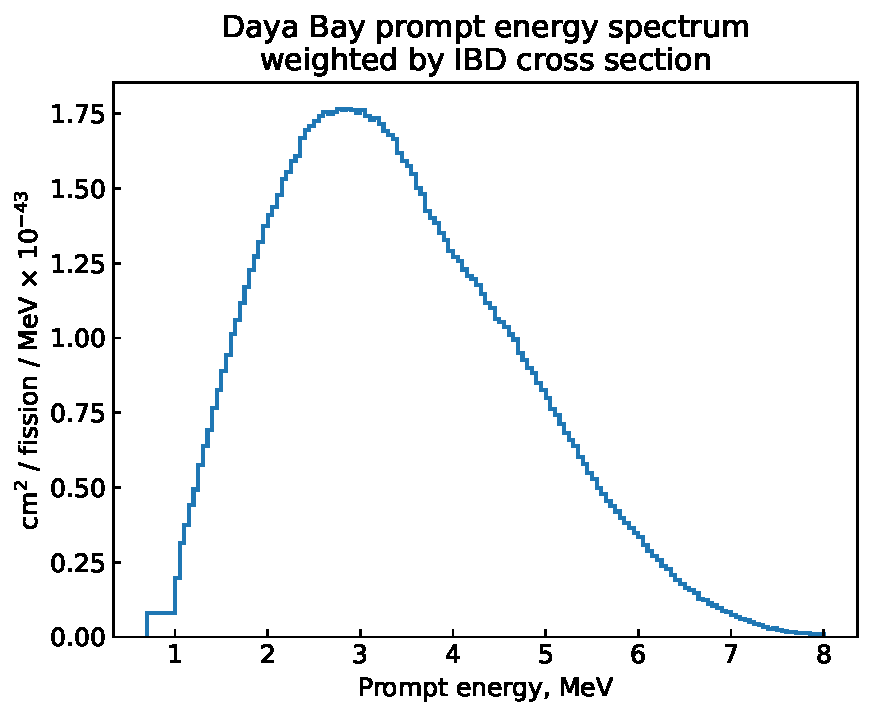
\includegraphics[width=\linewidth]{figs/Section2/dmitry_dyb_prompt_spectrum.pdf}
        \caption{Prompt energy spectrum}
        \label{fig:dyb_prompt_spectrum}
      \end{subfigure}
      \hfill
      \begin{subfigure}[t]{0.49\textwidth}
        \centering
        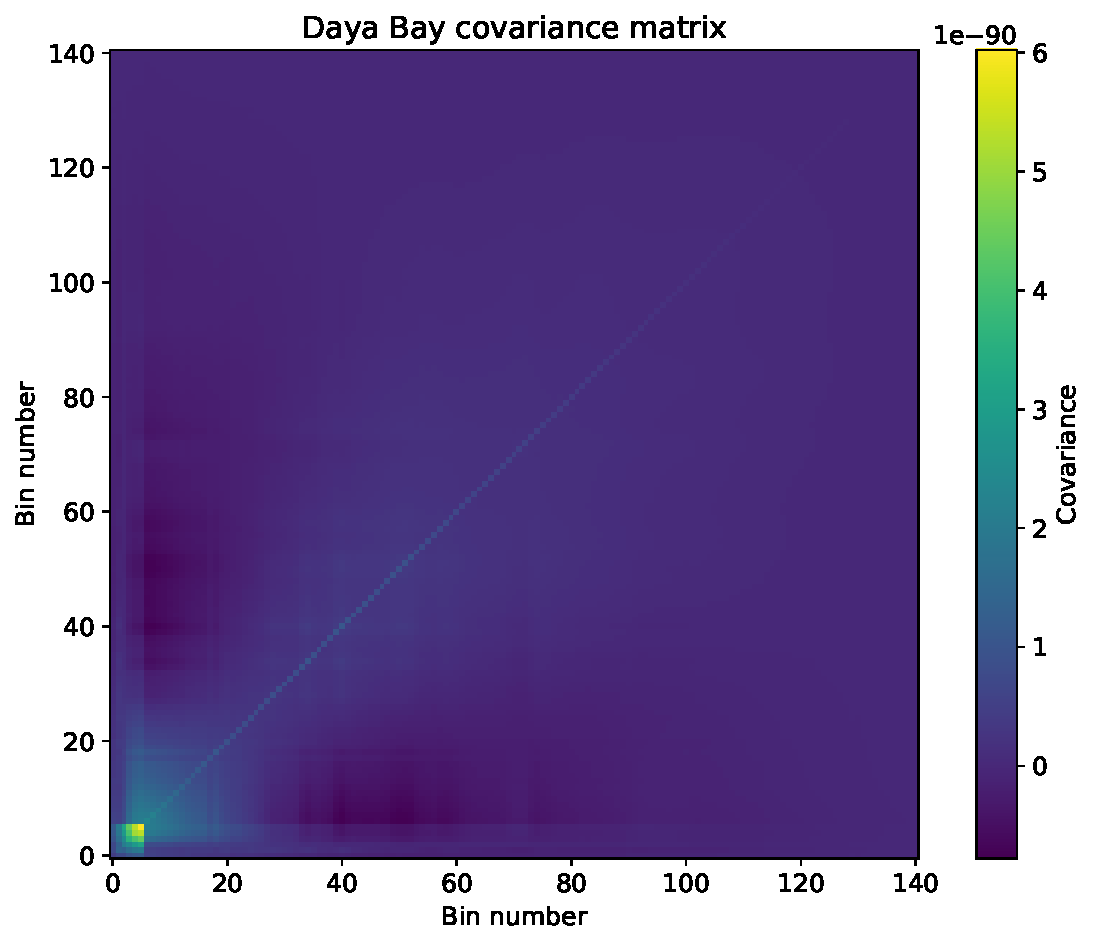
\includegraphics[width=\linewidth]{figs/Section2/dmitry_dyb_cov_mat.pdf}
        \caption{Covariance matrix}
        \label{fig:dyb_cov_mat}
      \end{subfigure}
      \caption{Daya Bay inputs}
      \label{fig:dyb_inputs}
    \end{figure}

  \item \textbf{Construction of a $\chi^2$ term for Daya Bay:}  The Daya Bay contribution to the
    total $\chi^2$ was constructed using the relative covariance matrix:
    \begin{equation}
      \chi^2_{\text{DYB}} = \sum_{i,j}^{141} \left(\frac{x_i}{\mu_i} - 1\right) Q_{ij}^{-1}
      \left(\frac{x_j}{\mu_j} - 1\right)
    \end{equation}
    where $x_i$ and $\mu_i$ are the observed and expected number of events in bin $i$.

  \item \textbf{Total $\chi^2$ for the combined fit:}  The total $\chi^2$ used in the combined fit
    includes JUNO, Daya Bay, and pull terms:
    \begin{equation}
      \chi^2 = \chi^2_{\text{JUNO}} + \chi^2_{\text{DYB}} + \chi^2_{\text{pulls}},
    \end{equation}


\end{enumerate}

It is also worth noting that the current model does not account for positron energy losses near the
Inner Acrylic Vessel (IAV), an effect present in Daya Bay. While this omission is assumed to have a
small impact at this stage, it should be addressed for more precise future analyses.

\subsubsection{Selection of Antineutrino Spectrum Model}
In a combined JUNO+Daya Bay analysis, both detectors must share the same underlying reactor
antineutrino spectrum model to allow Daya Bay to constrain its shape. To enable this, the
$\bar{\nu}_e$ spectrum is divided into segments whose normalization parameters are varied during
minimization.

Choosing the appropriate segmentation is crucial. On one hand, the segments must not be too small
because otherwise Daya Bay won't be able to resolve them due to strong correlations. Ideally, the
segments should be as wide as about 1.5$\sigma$ energy resolution width at given energy (see
Figure~\ref{fig:dyb_segments}). Given Daya Bay's energy resolution $\sigma$ of 8.5\% at 1 MeV, this
sets a lower limit on segment widths to $> 100$~keV across most of the spectrum.
\begin{figure}[H]
  \centering 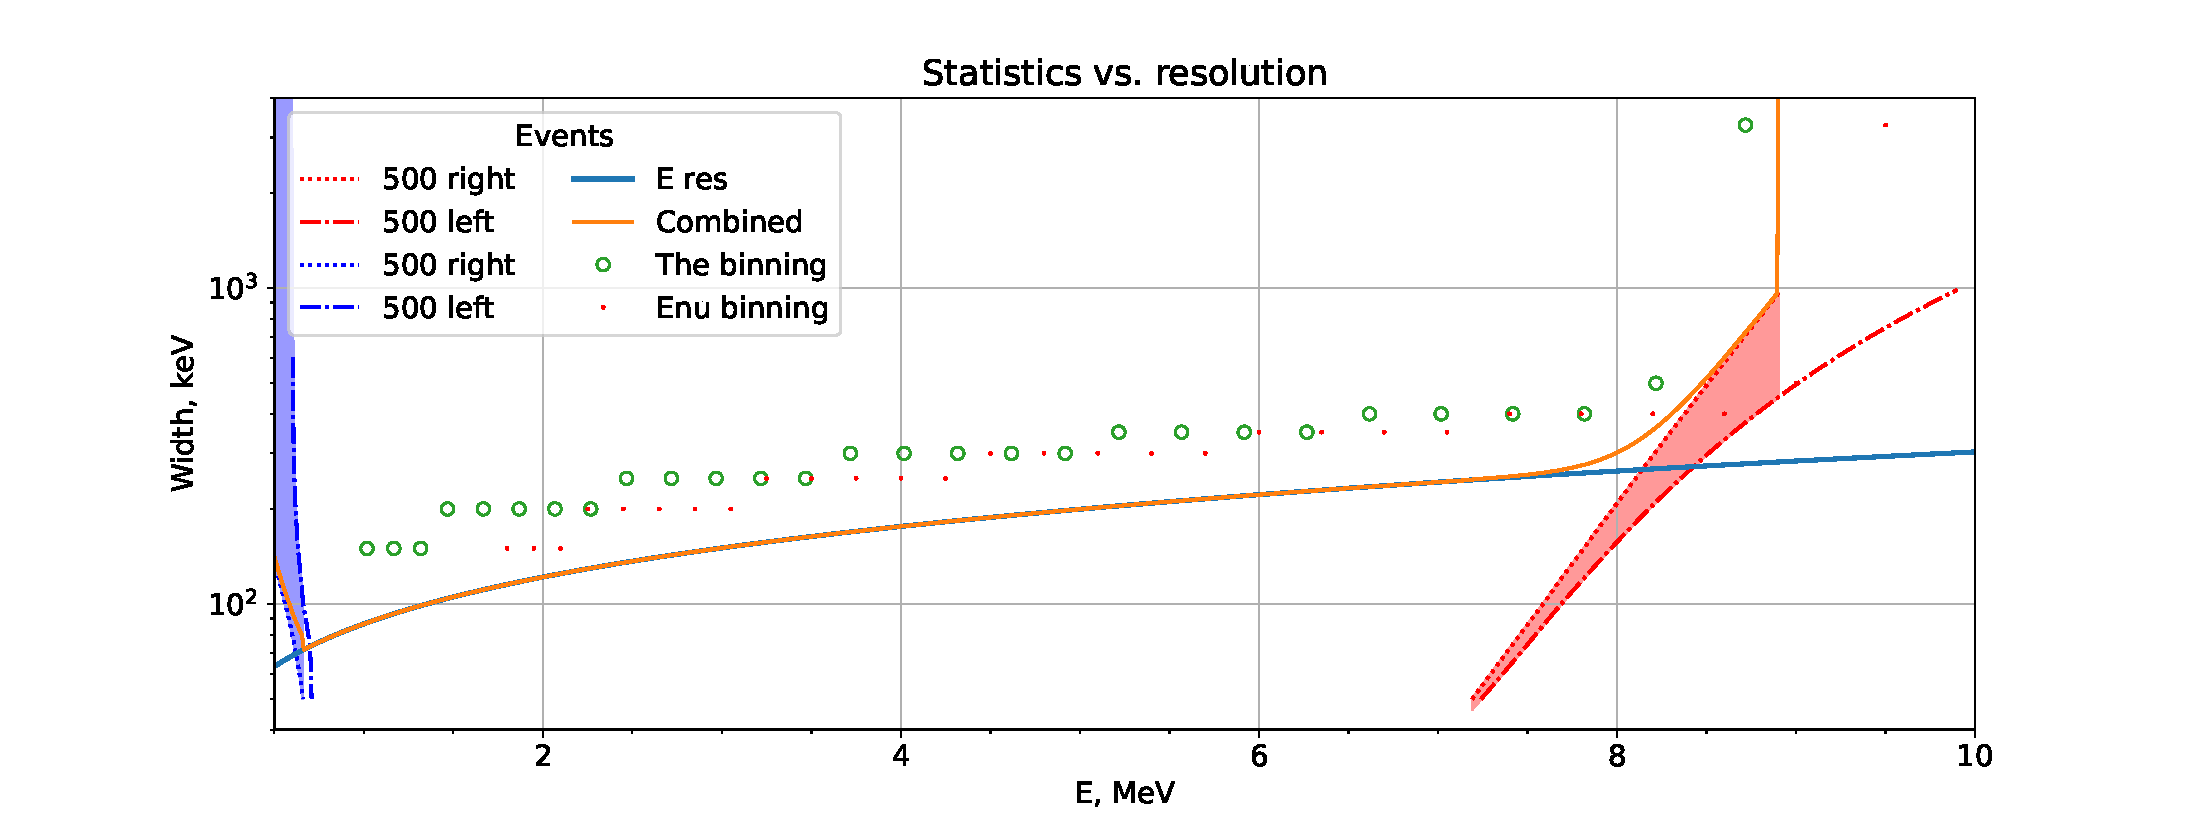
\includegraphics[width=0.99\textwidth]{figs/Section2/dmitry_dyb_segs.pdf}
  \caption{1.5$\sigma$ segmentation for Daya Bay energy resolution case.}
  \label{fig:dyb_segments}
\end{figure}

At the same time, accurate measurement of $\Delta m^2_{31}$ in JUNO requires resolving fine
oscillation pattern in the prompt energy spectrum. If the segment widths and the associated
detector binning are too large, they fail to capture these fast variations and result in degraded
sensitivity.

To balance these constraints, this study uses a segmentation scheme where the antineutrino spectrum
segments are matched to JUNO’s final prompt energy binning. Uniform bin widths of 100~keV in the
energy region from 1 to 7~MeV were chosen:
\newline\newline
JUNO final binning (68 bins): \hfill $0.8, 1_{+100}, ..., 7_{+300}, ..., 8.2, 12 \ [\text{MeV}_\text{+keV}]$
\newline\newline
which is a compromise between Daya Bay’s resolution limit and JUNO’s oscillation sensitivity.

This choice is rather empirical and not highly optimized.
Figure~\ref{fig:dm31_binning_vs_sensitivity} shows the relative uncertainty on $\Delta m^2_{31}$ as
a function of JUNO’s bin width, assuming the antineutrino spectrum is fixed (or perfectly known). As
the bins become wider, the sensitivity decreases. Conversely, using significantly finer bins would
require correspondingly finer segmentation, which Daya Bay cannot resolve reliably.
\begin{figure}[H]
  \centering 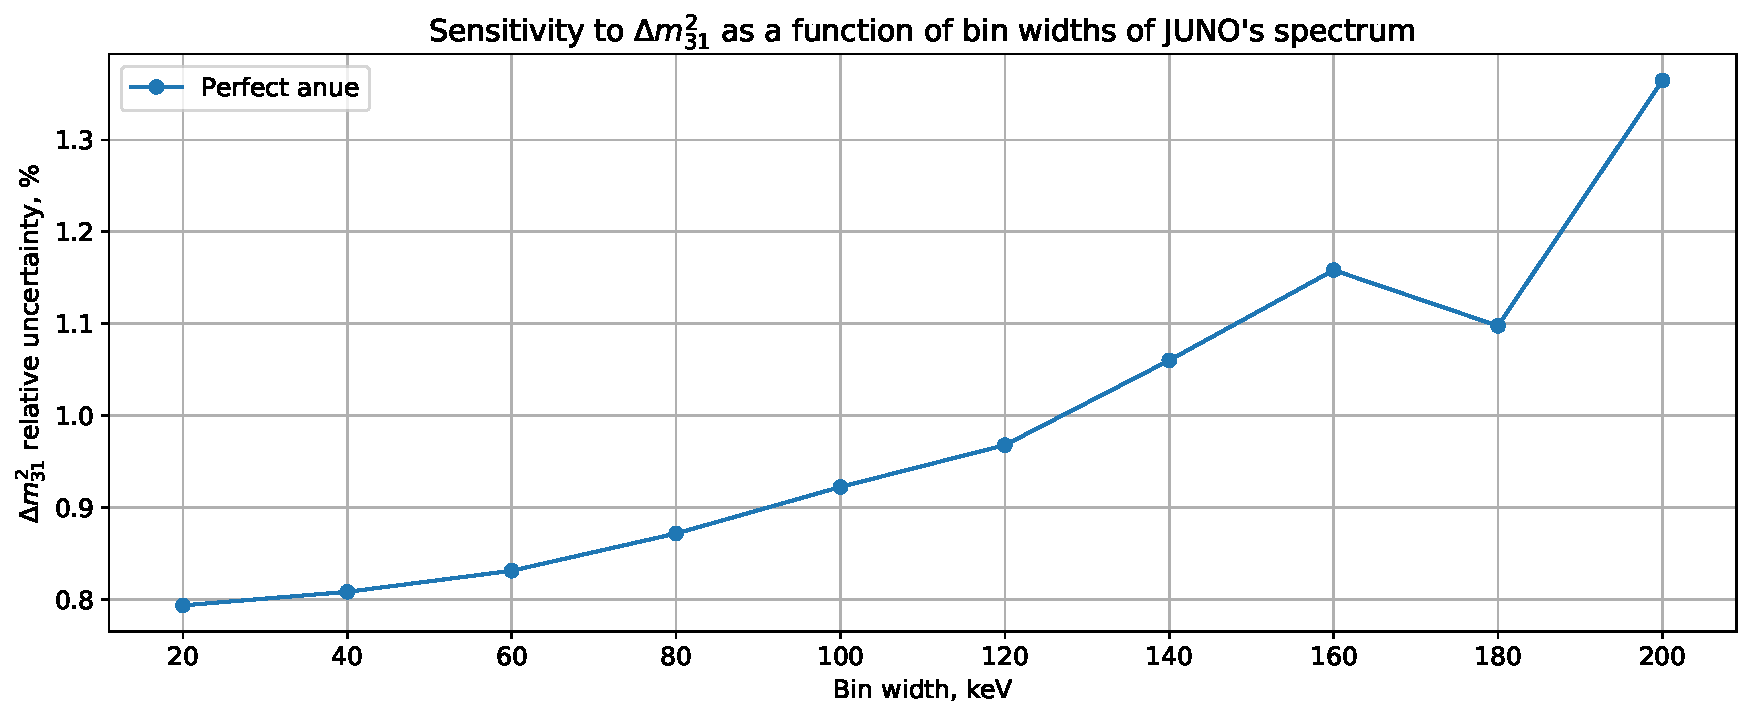
\includegraphics[width=0.99\textwidth]{figs/Section2/dmitry_dm31_binning_impact.pdf}
  \caption{JUNO's final binning impact on sensitivity to $\Delta m^2_{31}$}
  \label{fig:dm31_binning_vs_sensitivity}
\end{figure}

\subsection{Analysis Results}

\subsubsection{Asimov Study}
To evaluate baseline performance, we first estimate the relative uncertainties on oscillation
parameters using Asimov dataset. While we acknowledge that Asimov sensitivities may be unreliable in the low-statistics regime, especially for $\Delta m^2_{31}$, they still give a useful idea of how much the sensitivity might improve or degrade when using Daya Bay constraints instead of TAO. To explore this, we compare the JUNO+Daya Bay model with other approaches: JUNO+TAO, JUNO with bin-to-bin (b2b) antineutrino spectrum shape uncertainty, and JUNO with a fixed antineutrino spectrum. This helps us better understand how different assumptions affect the overall performance.

Table~\ref{tab:junodyb_asimov} shows comparison of JUNO+Daya Bay performance with other models.
Several features are worth highlighting:
\begin{itemize}
  \item \textbf{JUNO + DYB shows competitive performance:} \\
    Although Daya Bay has lower energy resolution compared to TAO, the combined JUNO+Daya Bay
    analysis achieves decent sensitivity to $\Delta m^2_{31}$ and performs better for $\Delta
    m^2_{21}$ and $\sin^2 2\theta_{12}$. This is mainly due to Daya Bay’s large data statistics
    (over 3.5 million IBD events) and its well-controlled systematics, particularly its smaller absolute efficiency uncertainty (1.2\%), which directly impacts the precision of rate-sensitive parameters. TAO’s superior energy resolution benefits spectral shape measurements, but its larger normalization uncertainty (10\%) limits its impact on parameters sensitive to overall event rates.

  \item \textbf{Bin-to-bin models are overly optimistic:} \\
    Both JUNO+ b2b Daya Bay and JUNO+b2b TAO models yield very similar precision on all oscillation
    parameters. However, these results are too optimistic, as they do not properly account for the
    realistic freedom in the reactor antineutrino spectrum shape and possible correlations between
    bins. As such, they underestimate the true systematic uncertainty, especially for $\Delta
    m^2_{31}$.

  \item \textbf{Fixed spectrum is an idealized scenario:} \\
    The configuration with a fixed reactor spectrum shows the best possible precision, but it is not
    achievable in practice. It serves as a lower bound on the sensitivity. Interestingly, the
    results from b2b models are nearly identical to this fixed-spectrum case, which confirms that
    they are too optimistic.
\end{itemize}

\begin{table}[H]
  \centering
  \caption{Relative uncertainties on oscillation parameters for 100 days of JUNO data taking time
  (Asimov case). JUNO+DYB and JUNO+TAO have the same antineutrino spectrum segmentation. All models
  have the same JUNO's final binning.}
  \label{tab:junodyb_asimov}
  \begin{tabular}{lccc} \toprule
    Configuration & $\Delta m^2_{31}$ (\%) & $\Delta m^2_{21}$ (\%) & $\sin^2 2\theta_{12}$ (\%) \\
    \midrule
    JUNO + DYB                 & 1.13 & 0.98 & 0.99 \\
    JUNO + TAO                 & 0.97 & 1.08 & 1.38 \\
    JUNO + b2b TAO             & 0.94 & 0.96 & 0.98 \\
    JUNO + b2b DYB             & 0.94 & 0.96 & 0.98 \\
    JUNO (fixed $\bar{\nu}_e$) & 0.93 & 0.96 & 0.98 \\
    \bottomrule
  \end{tabular}
\end{table}
®
This analysis highlights Daya Bay’s pragmatic strength: while energy resolution is modest compared
to TAO, its statistical power and well-controlled systematics make it a viable and stable constraint
for early-phase JUNO studies.

\subsubsection{ToyMC Study}
To evaluate the statistical performance of the JUNO+Daya Bay combined analysis and validate the
reliability of interval estimation, a Toy Monte Carlo (ToyMC) study was performed. The simulation
includes 5000 pseudo-experiments, each corresponding to 100 days of JUNO data taking time. In each
toy, all nuisance parameters (except the antineutrino spectrum segments) are randomized using
Gaussian distribution. Statistical and bin-to-bin fluctuations are then applied using the full
covariance matrix. The resulting pseudo experiments are used to extract the $\chi^2$ profile of
$\Delta m^2_{31}$, assuming a true value of $2.5413 \times 10^{-3}~\text{eV}^2$.

The 1$\sigma$ confidence intervals are obtained under the assumption of Wilks' theorem, using a critical threshold of $\Delta \chi^2=1$. The distribution of interval types observed in the toy experiments is shown in Figure~\ref{fig:interval_classification}. Several important features are evident:
\begin{itemize}
  \item In only 12.50\% of toys, a single 1$\sigma$ interval is found that both covers the true value
    and is narrower than the Asimov interval.
  \item A significant fraction (68.41\%) of toys result in either multiple intervals or a single
    interval that does not cover the true value.
  \item In particular, 35.7\% of toys yield a single interval that misses the true value, and 31.19\%
    produce multiple intervals with no coverage.
  \item The overall coverage rate, defined as the fraction of toys with at least one interval
    covering the true $\Delta m^2_{31}$, is only 31.59\%.
\end{itemize}

% TODO: replace jpg picture with pdf
\begin{figure}[H]
  \centering
  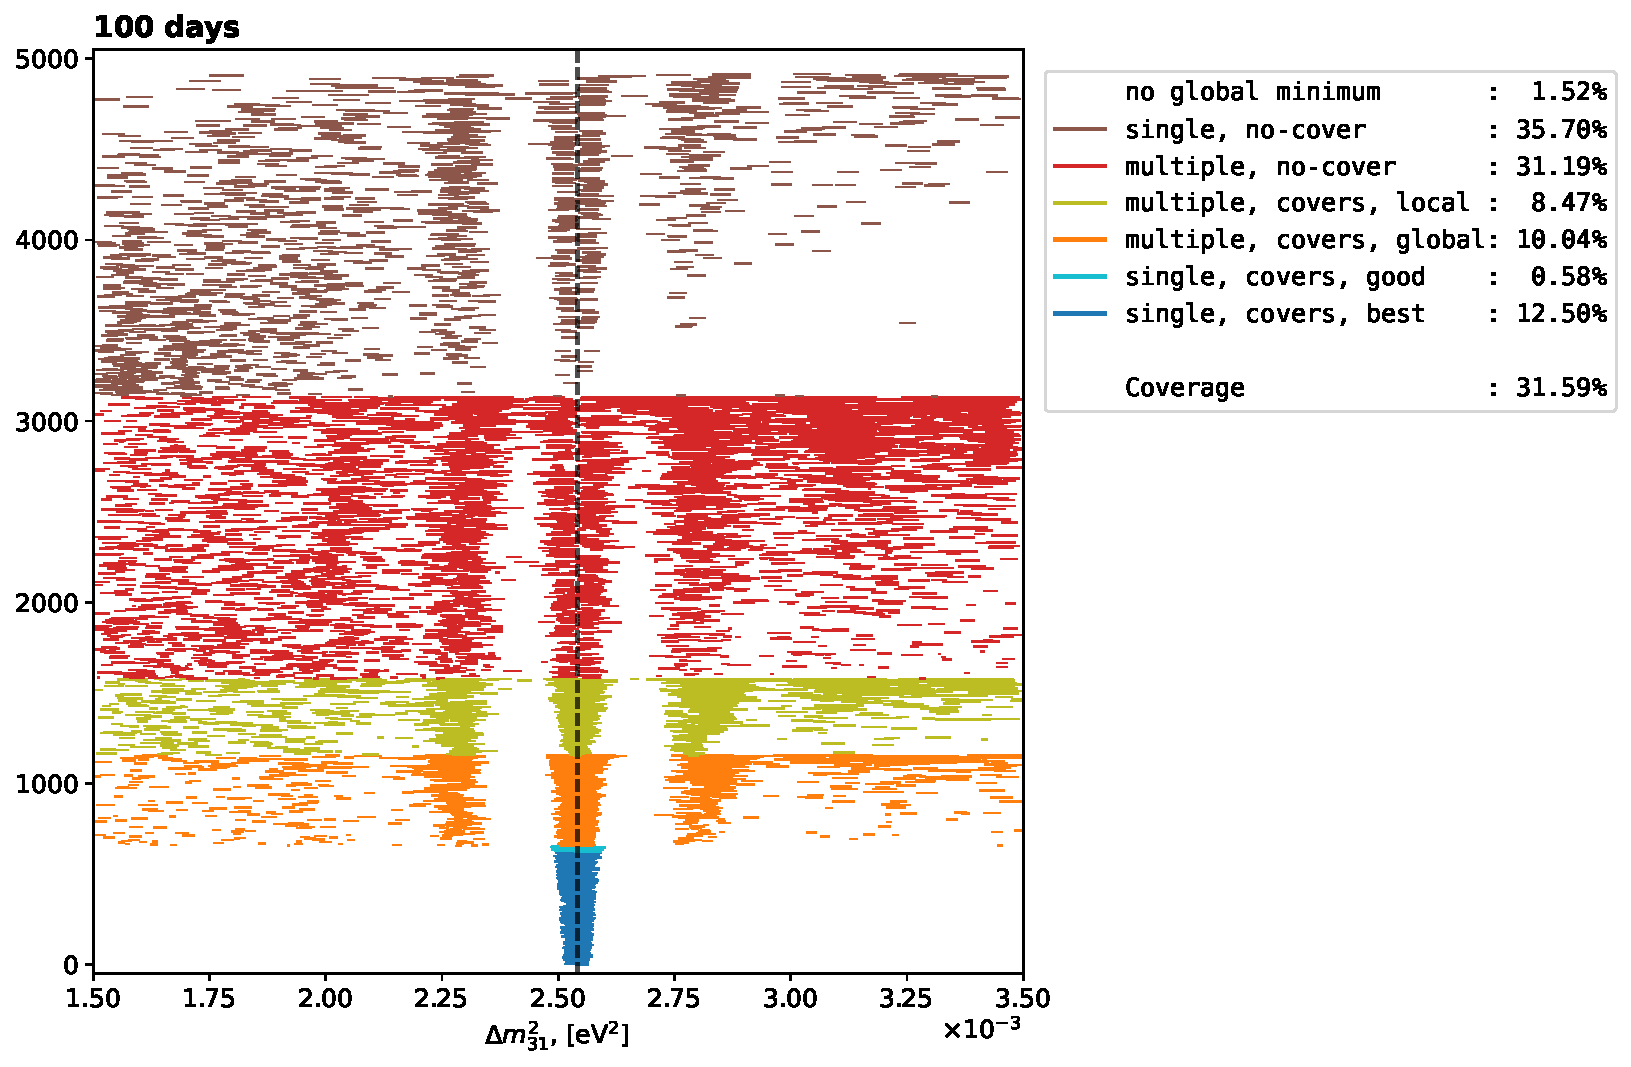
\includegraphics[width=0.95\linewidth]{figs/Section2/dmitry_junodyb_intervals.pdf}
  \caption{Classification of 1$\sigma$ intervals in 5000 ToyMC experiments obtained with JUNO+Daya
  Bay model.}
  \label{fig:interval_classification}
\end{figure}

\subsection{Conclusions of this Section}
This study shows that Daya Bay data can be effectively used to constrain the reactor antineutrino
spectrum in JUNO’s first oscillation analysis. Since TAO data are unlikely to be available in time,
Daya Bay provides a viable input for early measurements. Although the JUNO+Daya Bay configuration
yields slightly worse sensitivity to $\Delta m^2_{31}$ compared to JUNO+TAO, it achieves comparable
or better precision for other parameters, such as $\Delta m^2_{21}$ and $\sin^2 2\theta_{12}$, due
to Daya Bay’s high statistics and well-controlled detector normalization.

ToyMC studies indicate that confidence intervals defined using the $\Delta\chi^2 = 1$ approximation
tend to underestimate true uncertainties. This highlights the need for a more robust statistical
treatment, such as the Feldman–Cousins approach.

Looking ahead, a combined analysis incorporating JUNO, TAO, and Daya Bay data may offer improved
sensitivity by leveraging complementary strengths. In such a configuration, Daya Bay can help
constrain the initial antineutrino spectrum shape, which, together with TAO’s fine energy
resolution, can enhance overall sensitivity to all oscillation parameters.

% \begin{itemize}
%     \item Brief introduction: remind that toy generation is the same as previous sections.
%     \item Main results
%     \begin{itemize}
%     \item Show that $\Delta m^2_{21}$ and $\sin^2 \theta_{12}$ best fit distributions are gaussian or equivalently that $\Delta\chi^2$ profiles are $\sim$ parabolic even at (very) low exposure (30-50 days). 
%     \item Precision and bias studies, comparison between different cost functions.
%     \end{itemize}
%     \item Conclusions
%     \begin{itemize}
%     \item There are no evident show-shoppers for a low-stats measurement of solar parameters
%     \end{itemize}

% \end{itemize}



\section{Impact on the NMO Determinations of Other Experiments}\label{sec:nmoimpact}

%\item Brief intro to motivation of inspecting potential boost on LBL NMO from JUNO constraints%(several sentence,reference)
\subsection{Motivation} %(Junjie)
As discussed in Stephen J. Parke's paper~\cite{Parke:2024xre}, the potential of resolving mass ordering at 3$\sigma$ confidence level is exciting when combining the atmospheric mass splitting from the muon neutrino disappearance channels of long baseline experiments, i.e. T2K and NOvA in particular, with JUNO unprecedented precision from the electron anti-neutrino channel using only one year of data taking. Thus, it is necessary to evaluate the boost on mass ordering determination for long baseline experiments from JUNO's results as an external constraint. In the following sub-sections, we present the modeling and results from two different methods and end with a discussion on the result differences and caveats.
%model 搭建长基线模型（怎么复现实验结果）
%\item Description of approximation to LBL experiment models (T2K: Rongping and Junjie, NOvA: Rongping);
\subsection{Approximated modeling of LBL}

%%%%%%%%%%%%%%%
% 1. Spectrum-oriented method (Rongping)
%     1.1 Brief description of the method with the key formula (can use T2K as an example)
%     1.2 Show plots (comparison of spectrum/chi2/etc. between published data of LBL and the method) [Both T2K and NOvA]
%
% 2. GLoBES method (Junjie)
%     2.1 Biref intro to GLoBES
%     2.2 Show plots
%%%%%%%%%%%%%%
In this sub-section, we mainly focus on the approximation of T2K (and NOvA in one of the methods) using two methods. A beam of (anti-)muon neutrinos is produced at J-PARC and travels 295~km to be detected at the water Cherenkov detector Super-Kamiokande (SK). A magnetic horn is designed to change the direction of the  magnetic field that focuses the mesons that produce the (anti-)neutrino beams. Thus, T2K is able to switch between neutrino mode and anti-neutrino mode, which is usually referred to as FHC (Forward Horn Current) and RHC (Reverse Horn Current). $\nu_{\mu}$($\bar{\nu}_{\mu}$) disappearance channels are sensitive to atmospheric mass splitting $|\Delta m_{32}^2|$. Similar to T2K, the far detector of NOvA aims to detect the $\nu_e$($\bar{\nu}_e$) appearance and $\nu_{\mu}$($\bar{\nu}_{\mu}$) disappearance channels from the $\nu_{\mu}$($\bar{\nu}_{\mu}$) beams produced at NuMI. 

\subsubsection{Spectrum-oriented method}
This section introduces how to reproduce the results of T2K and NOvA, so that the spectrum is as consistent as possible with the officially released spectrum, and at the same time, the fitting results are as consistent as possible with the officially announced results.

Firstly , there is the replication process of the T2K experiment.The T2K has two modes, $\nu$-mode  and $\bar{\nu}$-mode. Each mode can produce two signals, $\mu$-like and $e$-like. The interaction types involved in each signal are shown in \autoref{tab:t2k_samples}. The reproduction of this experiment is mainly based on the following formula.
\begin{equation}
S_{\text{predict}} = N \cdot \sum_{E_\nu \text{ bin}} \mathrm{F}(E_\nu) \mathrm{P}_{\alpha\beta}(E_\nu) \mathrm{Xsec}(E_\nu) \epsilon(E_\nu) R(E_{\text{rec}}, E_\nu) \epsilon_{\text{ND}}(E_{\text{rec}})
\end{equation}

\begin{itemize}
    \item $N$ is a constant factor used to normalize the predicted event rate such that the total number of events in the reproduced spectrum matches the total number observed in the T2K experiment.
    \item $\mathrm{F}(E_\nu)$ is the outgoing neutrino flux.
    \item $\mathrm{P}_{\alpha\beta}(E_\nu)$ is the oscillation probability.
    \item $\mathrm{Xsec}(E_\nu)$ is the cross section.
    \item $\epsilon(E_\nu)$ is the selection efficiency  
    \item $R(E_{\text{rec}}, E_\nu)$ is the energy smearing matrix with Gaussian distribution:  
    \[
    R(E_{\text{rec}}, E_\nu) = \frac{1}{\sqrt{2\pi}\sigma} \exp\left(-\frac{(E_{\text{rec}} - \text{scale} \cdot E_\nu)^2}{2\sigma^2}\right)
    \]  
    \[
    \sigma = a\sqrt{E_\nu} + b %\ (\text{further tuning about } a,b,\text{scale is expected})
    \]  
    \item $\epsilon_{\text{ND}}(E_{\text{rec}})$ is the constraints of the near detector on flux and cross-section.    
\end{itemize}

In the above formula, $N$, $\epsilon(E_\nu)$, $R(E_{\text{rec}}, E_\nu)$, $\epsilon_{\text{ND}}(E_{\text{rec}})$ are channel dependence.  


\begin{table}[!htp]
\centering
\begin{tabular}{|c|c|c|}
\hline
 & $\mu$-like & $e$-like \\%\multirow{2}{*}{$\nu$-mode} 
\hline
& $CCQE$ & $CCQE$ \\
\cline{2-3} 
          $\nu$-mode                  & $CC1\pi$ & $CC1\pi$ \\
\hline
$\bar{\nu}$-mode & $CCQE$ & $CCQE$ \\
\hline
\end{tabular}
\caption{Table of Event Types in the T2K Experiment}
\label{tab:t2k_samples}
\end{table}

The expected spectrum derived from the above formula and the officially released spectrum are shown in \autoref{fig:spec_t2k_zrp}. From this figure, it can be observed that the reproduced expected spectrum is in good agreement with the official energy spectrum.
\begin{figure}[H]
    \centering
    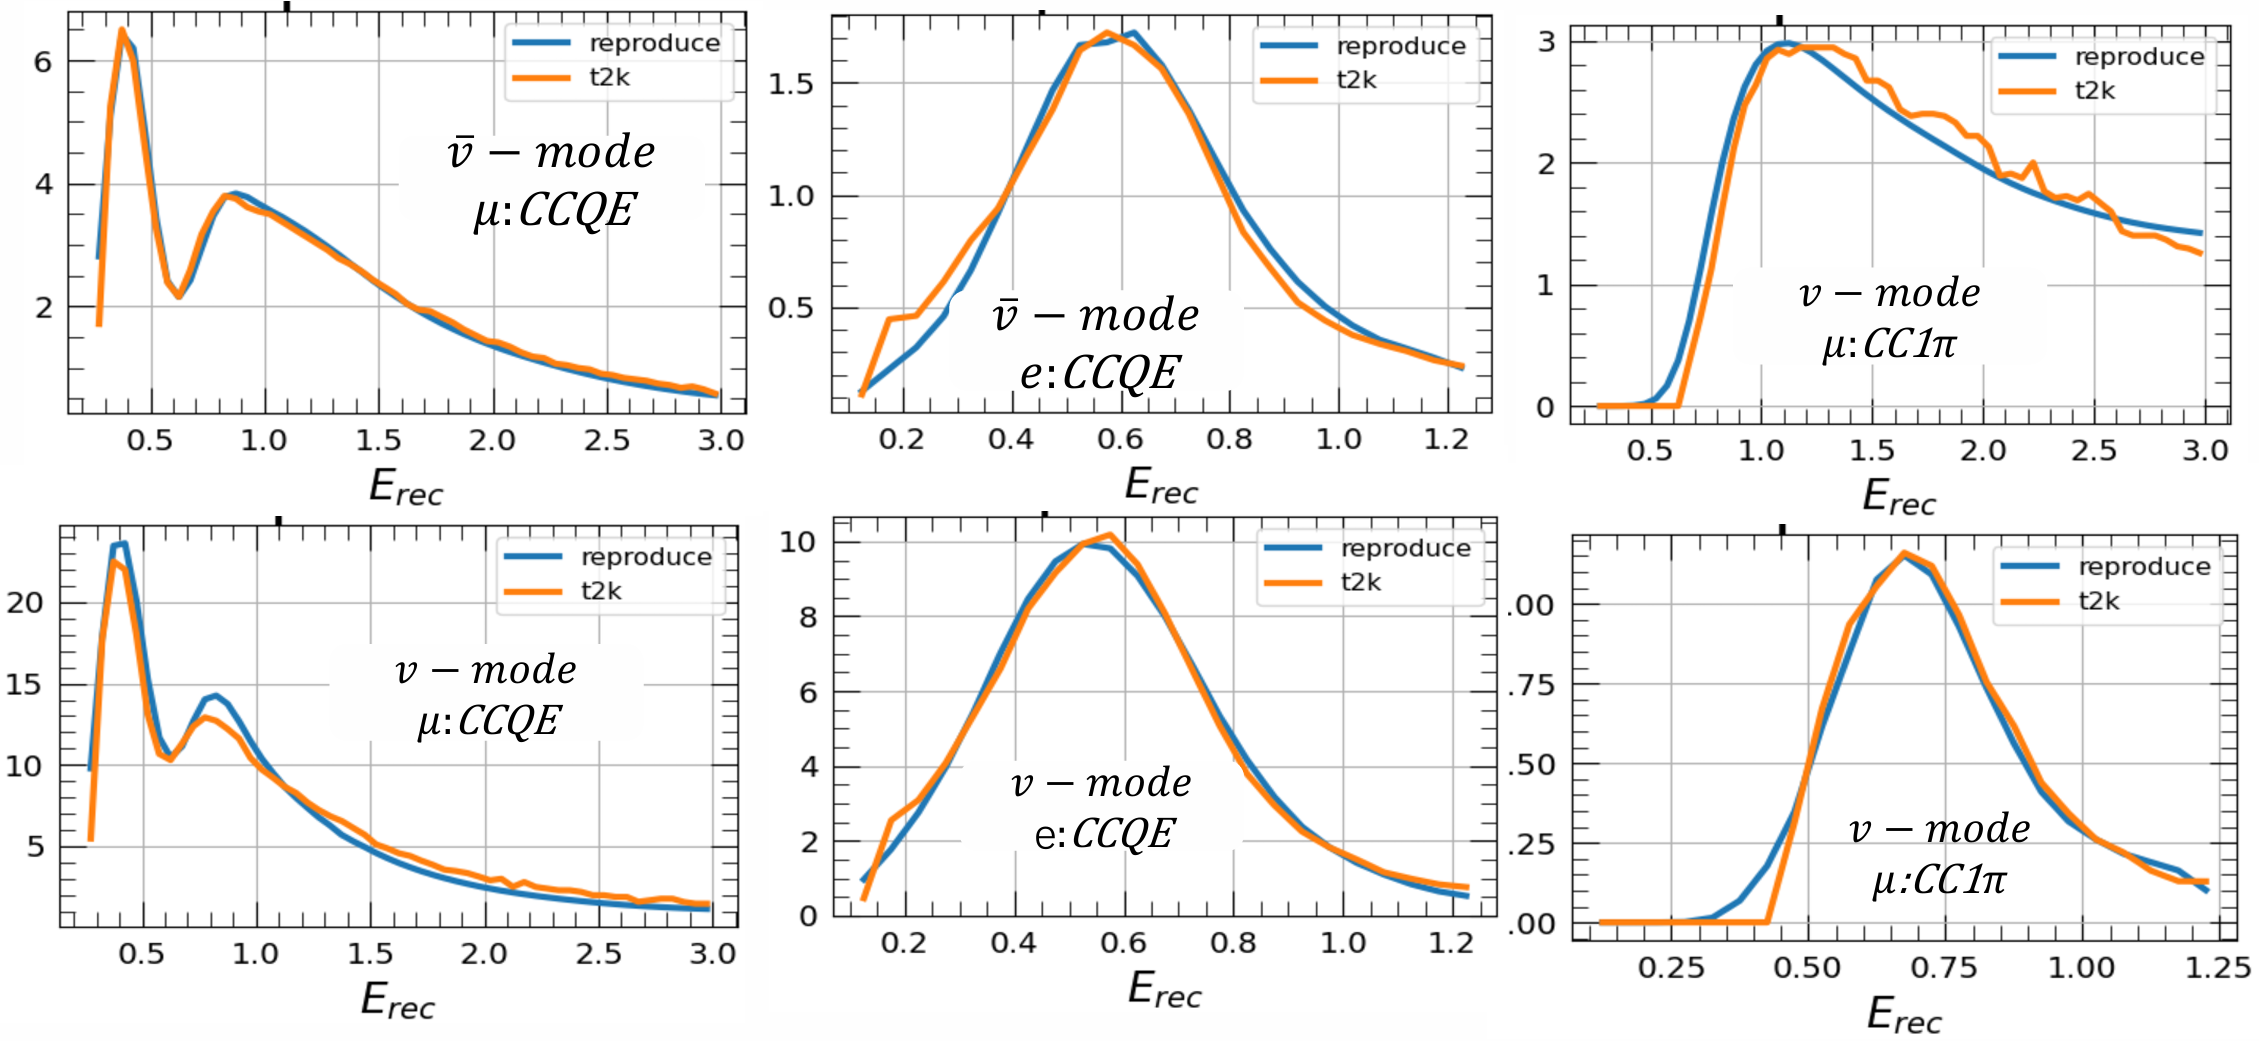
\includegraphics[width=0.8\linewidth]{figs//Section2//section2.6_Rongping_Junjie/spec_t2k_zrp.png}
    \caption{Expected spectra of T2K. The blue line represents the reproduced energy spectrum, and the orange line represents the officially released energy spectrum. }
    \label{fig:spec_t2k_zrp}
\end{figure}

The next step is to establish a minimization function to fit and obtain the optimal values and errors of the oscillation parameters. After introducing spectral shape and event rate uncertainty, the minimization function can be written as :
\begin{equation}
    \chi^2 = 2 \cdot \sum_{i} \sum_{\text{bin}} \left( sig_i - obs_i + obs_i \cdot \ln\left( \frac{obs_i}{sig_i} \right) \right) + \text{pull terms}
    \end{equation}
    where 
    \[
    sig_i = pre_i \cdot (1 + \alpha_{i,\text{bin shape}}) \cdot (1 + \alpha_{i,\text{rate}}) + bkg_i
    \]
\begin{itemize}
    \item $i=1,2\ldots,6$ means six samples  
    \item shape uncertainty is from post fit with ND constraints, it's bin-to-bin uncorrelated  
\end{itemize}
It should be noted that the function incorporates the reactor constraint $\theta_{13}$ (PDG 2024~\cite{ParticleDataGroup:2024cfk}), and we determine the confidence level (C.L.) using Wilks' theorem, whereas T2K employs the Feldman-Cousins method for C.L. determination. The fit results are listed in Table~\ref{tab:t2k_params}, it can be seen that the difference in \(\delta_{CP}\) between the reproduced and official results is \(0.2\sigma\), the difference in \(\Delta m^2_{32}\) is \(0.6\sigma\), and the difference in \(\sin^2\theta_{23}\) is \(0.025\).
\begin{table}[!ht]
\centering
\begin{tabular}{cccc}
\toprule
 & Reproduce & neutrino 2024 & Difference \\
\midrule
$\delta_{CP}$ 
  & $-1.96_{-0.73}^{+1.07}$ 
  & $-2.08_{-0.61}^{+1.33}$ 
  & $0.2\sigma$ ($\sigma=0.61$) \\

$\Delta m^2_{32}$ 
  & $2.496_{-0.033}^{+0.038} \times 10^{-3}\,\text{eV}^2$ 
  & $2.521_{-0.050}^{+0.037} \times 10^{-3}\,\text{eV}^2$ 
  & $0.68\sigma$ ($\sigma=0.037$) \\

$\sin^2\theta_{23}$ 
  & $0.543_{-0.085}^{+0.032}$ ($90\%$) 
  & $0.568_{-0.125}^{+0.024}$ ($90\%$) 
  & $0.025$ \\
\bottomrule
\end{tabular}
\caption{Comparison of fitted oscillation parameters between the approximated model and T2K's results from Neutrino 2024.}
\label{tab:t2k_params}
\end{table}

\subsubsection{GLoBES-based method}
%GLoBES: probably give some application examples...
General Long Baseline Experiment Simulator (GLoBES)~\cite{Huber:2004ka} is an open source package for researchers to simulate long baseline and reactor neutrino experiments. It allows users to define the neutrino fluxes, cross sections, signal and background compositions in samples and detector systematics. For oscillation calculations and $\Delta \chi^2$ extractions, GLoBES has both the built-in functions and flexibility for users to define their own calculations. More detailed information can be found in the official website~\cite{Huber:2004ka}.
%Dump plots here for GLoBES-T2K spectra and chi2 comparisons
In this GLoBES-based method, we aimed to approximate the data spectra released in T2K 2020 oscillation analysis (ref.) (T2K OA2020). The FHC 1R e-like, RHC 1R e-like, FHC 1R $\mu$-like and RHC 1R $\mu$-like. "1R" refers to the Cherenkov ring produced by the outgoing lepton, i.e. electron or muon. "e($\mu$)-like" refers to the ring PID determined by the reconstructed algorithm. For simplicity, we only focused on the above-mentioned four single ring samples in GLoBES-method. The data spectra and (anti-)neutrino fluxes are obtained from the published data set in the T2K OA2020 (ref). Cross section look-up tables are extracted from (ref).  Only charged current quasi-elastic (CCQE), charged current non quasi-elastic (CCnonQE) and neutral current (NC) are considered. The same detection efficiencies of different compositions in each sample are used as (ref). A set of co-efficiencies that account for the other systematics were fine-tuned by comparing to the data spectra. \autoref{t2kjuno_junjie:spectra_comparison} shows the comparison between the T2K OA2020 spectra and the re-production of the GLoBES-based method for both mass orderings.
\begin{figure}[H]
    \centering
    \begin{subfigure}[t]{0.22\textwidth}
    \centering
    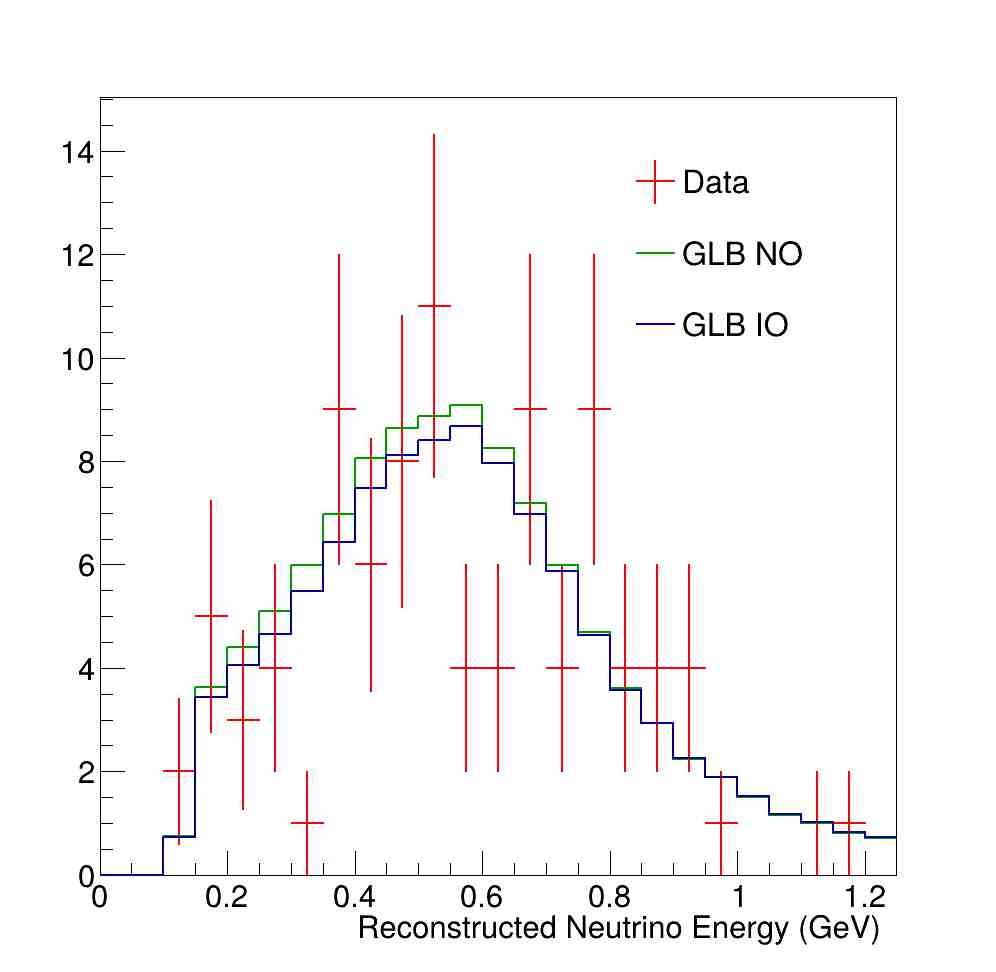
\includegraphics[width=\linewidth]{figs/Section2/section2.6_Rongping_Junjie/globes_t2k_fhc1re.jpg}
    \caption{FHC 1R e-like sample}
    \end{subfigure}
    \begin{subfigure}[t]{0.22\textwidth}
    \centering
    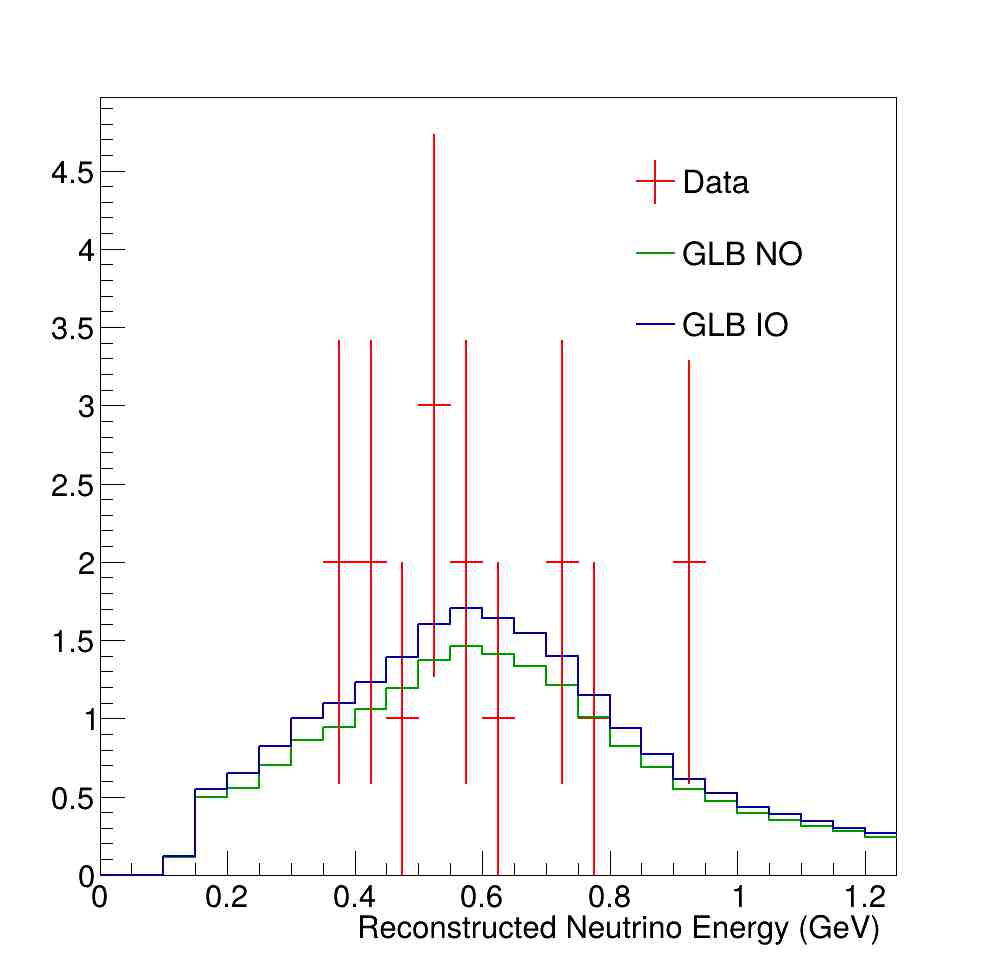
\includegraphics[width=\linewidth]{figs/Section2/section2.6_Rongping_Junjie/globes_t2k_rhc1re.jpg}
    \caption{RHC 1R e-like sample}
    \end{subfigure}
    \begin{subfigure}[t]{0.22\textwidth}
    \centering
    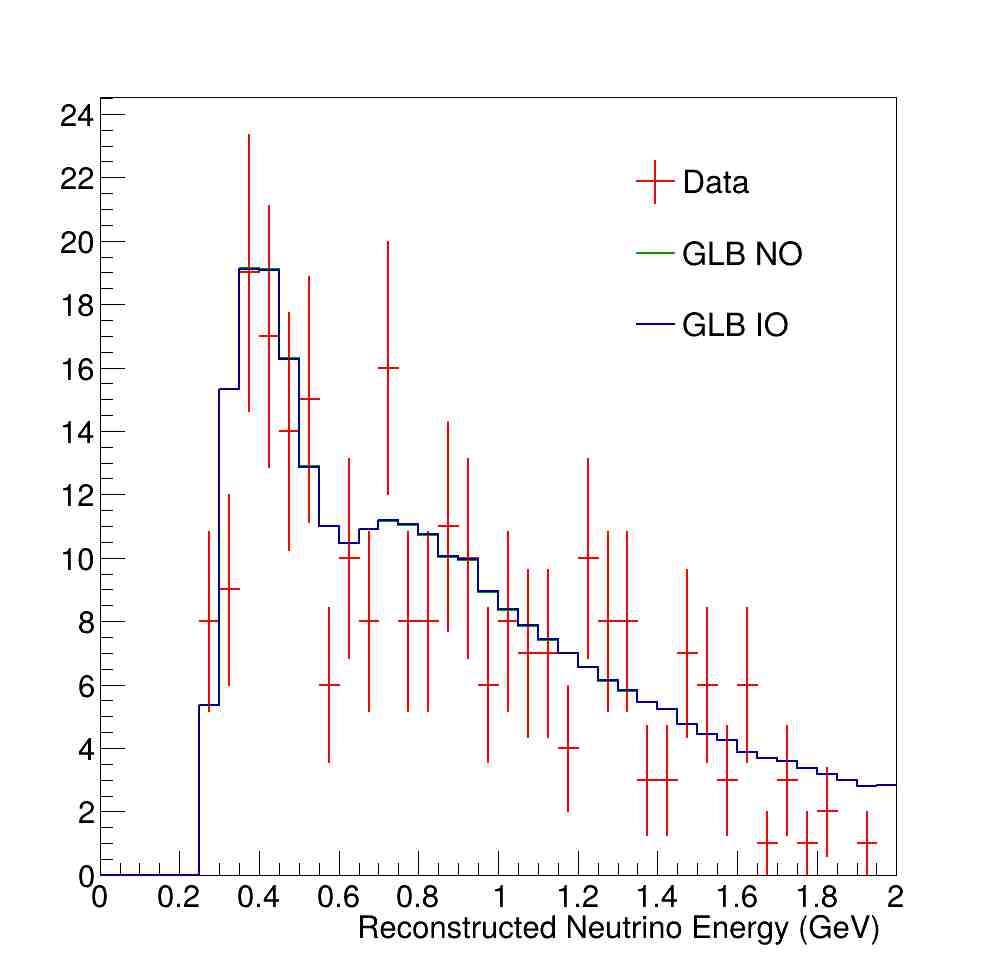
\includegraphics[width=\linewidth]{figs/Section2/section2.6_Rongping_Junjie/globes_t2k_fhc1rmu.jpg}
    \caption{FHC 1R $\mu$-like}
    \end{subfigure}
    \begin{subfigure}[t]{0.22\textwidth}
    \centering
    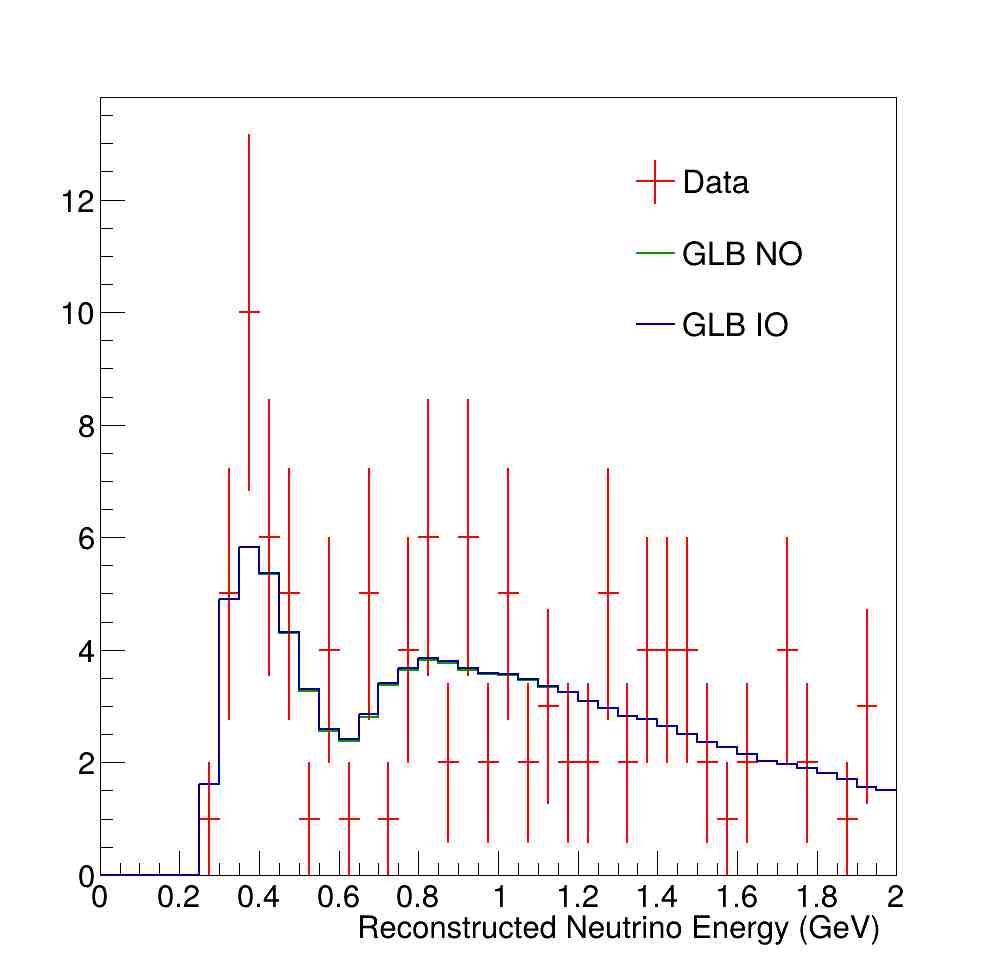
\includegraphics[width=\linewidth]{figs/Section2/section2.6_Rongping_Junjie/globes_t2k_rhc1rmu.jpg}
    \caption{RHC 1R $\mu$-like}
    \end{subfigure}
    \caption{Sample spectra comparison of four target samples between GLoBES-T2K and T2K published data. Red data points are from T2K official oscillation analysis in 2020 (ref). Both normal and inverted ordering assumptions are plotted for GLoBES-based method.}
    \label{t2kjuno_junjie:spectra_comparison}
\end{figure}

Besides the spectra comparison, the comparison of $\Delta\chi^2$ for the oscillation parameters of interest is also plotted, see \autoref{t2kjuno_junjie:chi2_comparison}. Though not perfect agreement, but good agreement is achieved around the minimum $\Delta\chi^2$ area. 

\begin{figure}[H]
    \centering
    \begin{subfigure}[t]{0.22\textwidth}
        \centering
        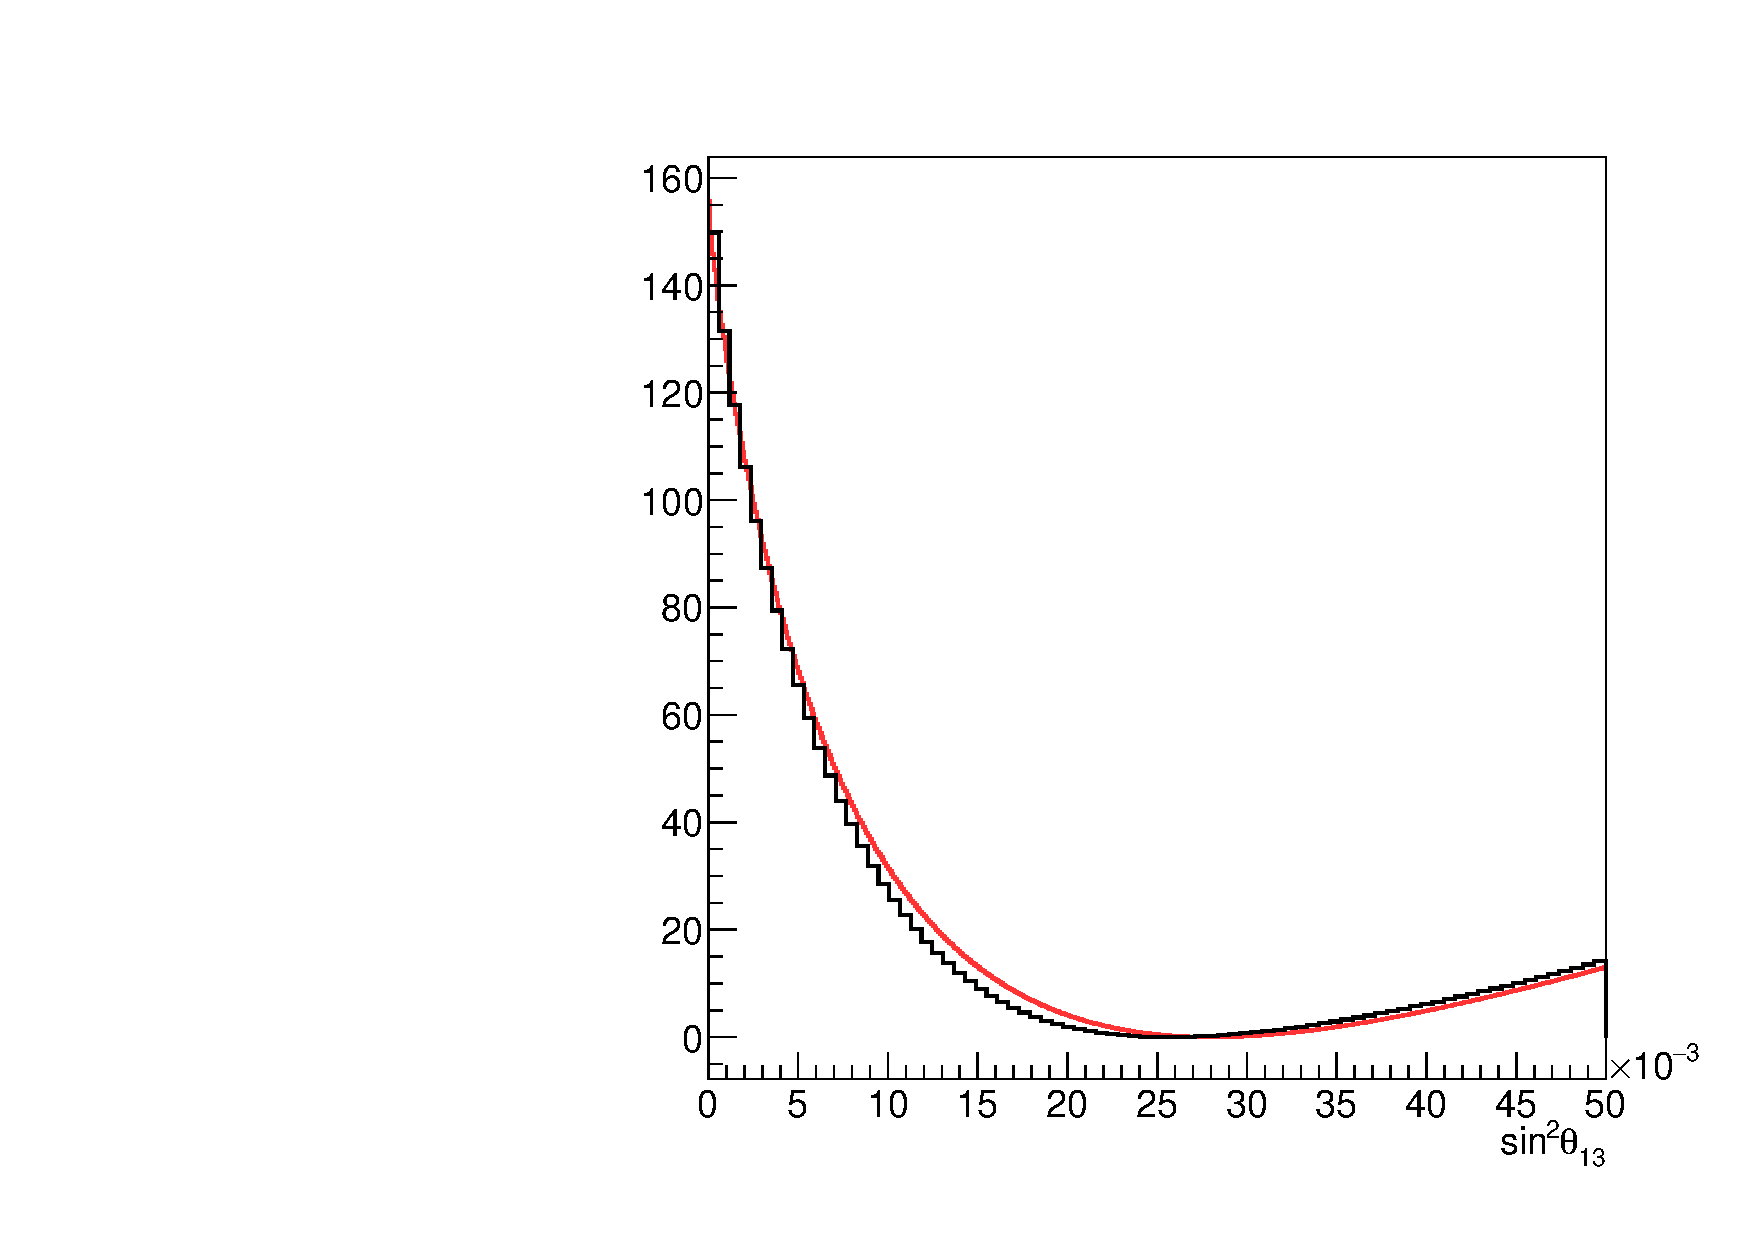
\includegraphics[width=\linewidth]{figs/Section2/section2.6_Rongping_Junjie/globes_t2k_chi2_th13_comparison_no.pdf}
        \caption{$\Delta\chi^2$ of $\sin{\theta_{13}}^2$}
    \end{subfigure}
    \begin{subfigure}[t]{0.22\textwidth}
        \centering
        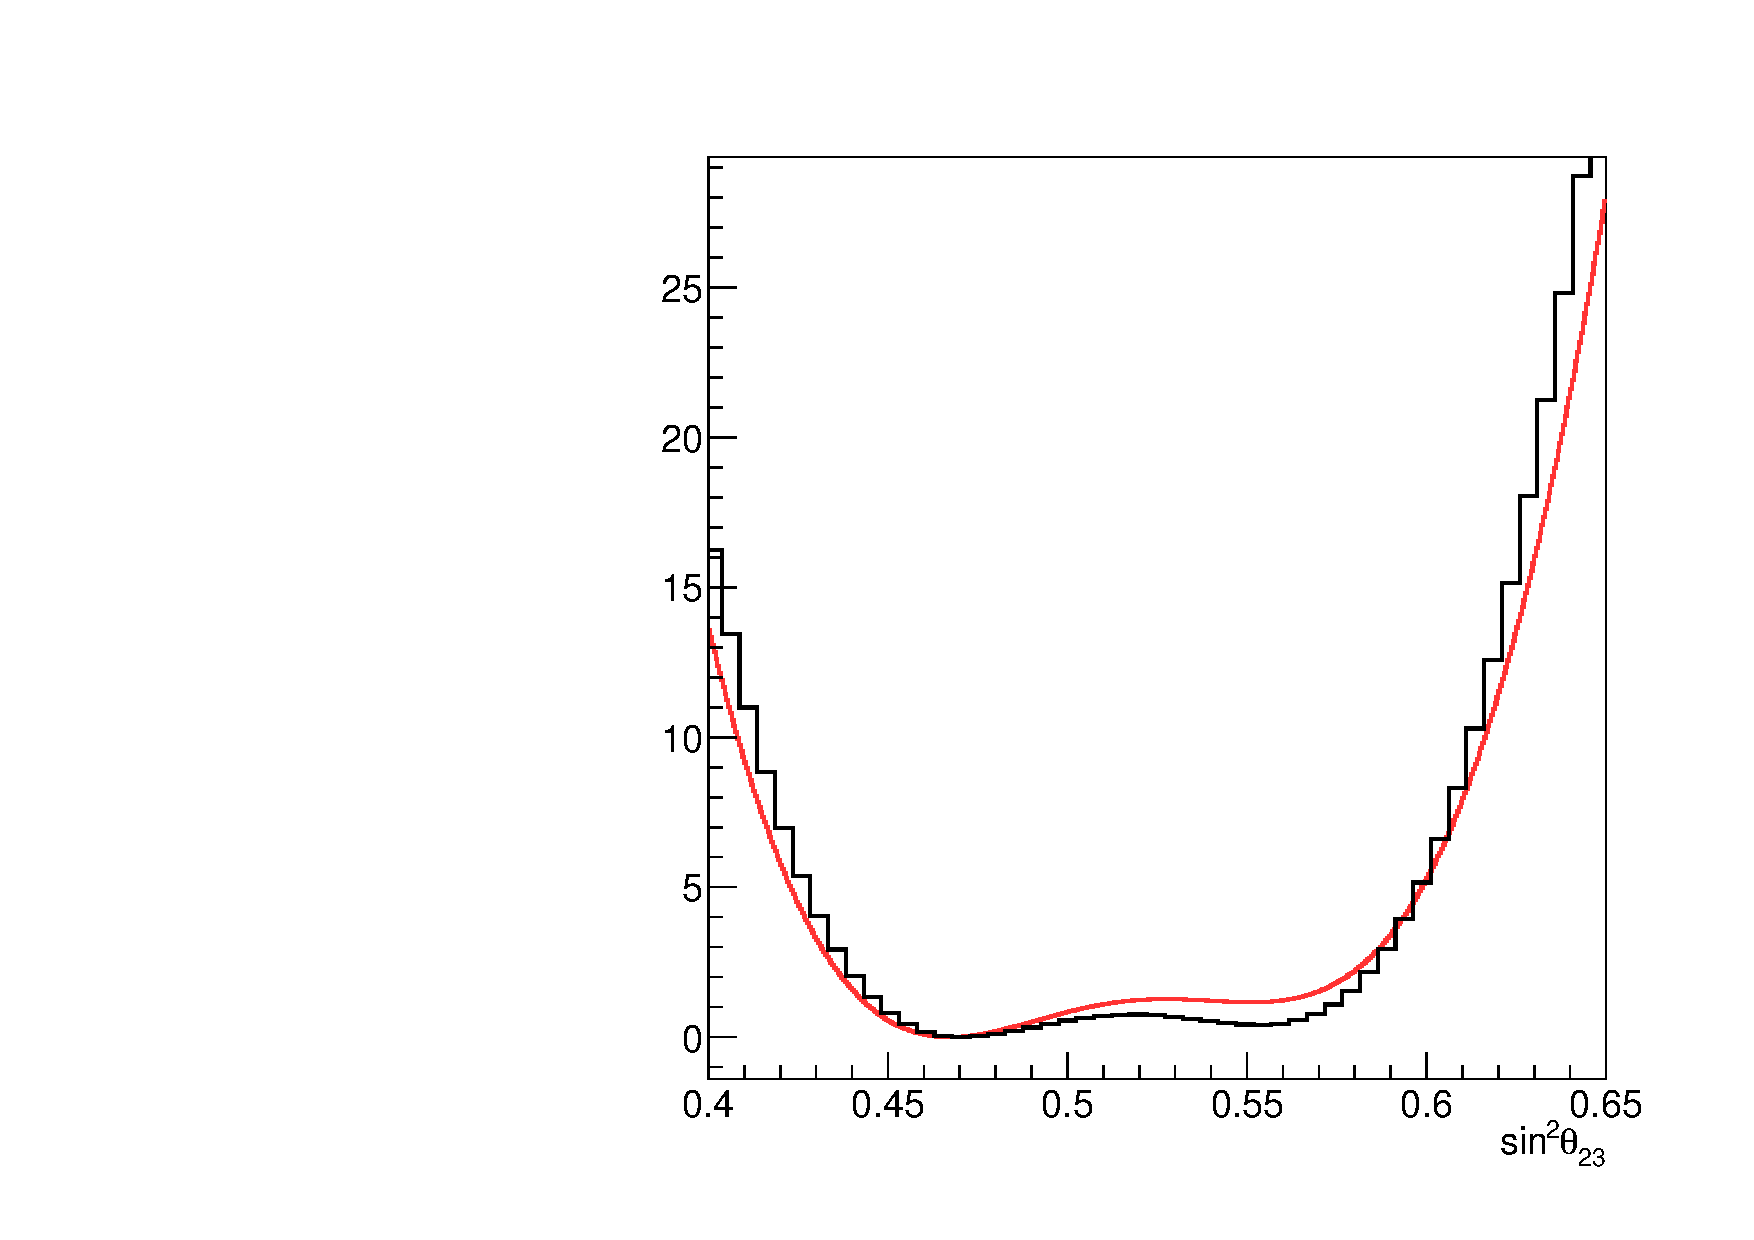
\includegraphics[width=\linewidth]{figs/Section2/section2.6_Rongping_Junjie/globes_t2k_chi2_th23_comparison_no.pdf}
        \caption{$\Delta\chi^2$ of $\sin{\theta_{23}}^2$}
    \end{subfigure}
    \begin{subfigure}[t]{0.22\textwidth}
        \centering
        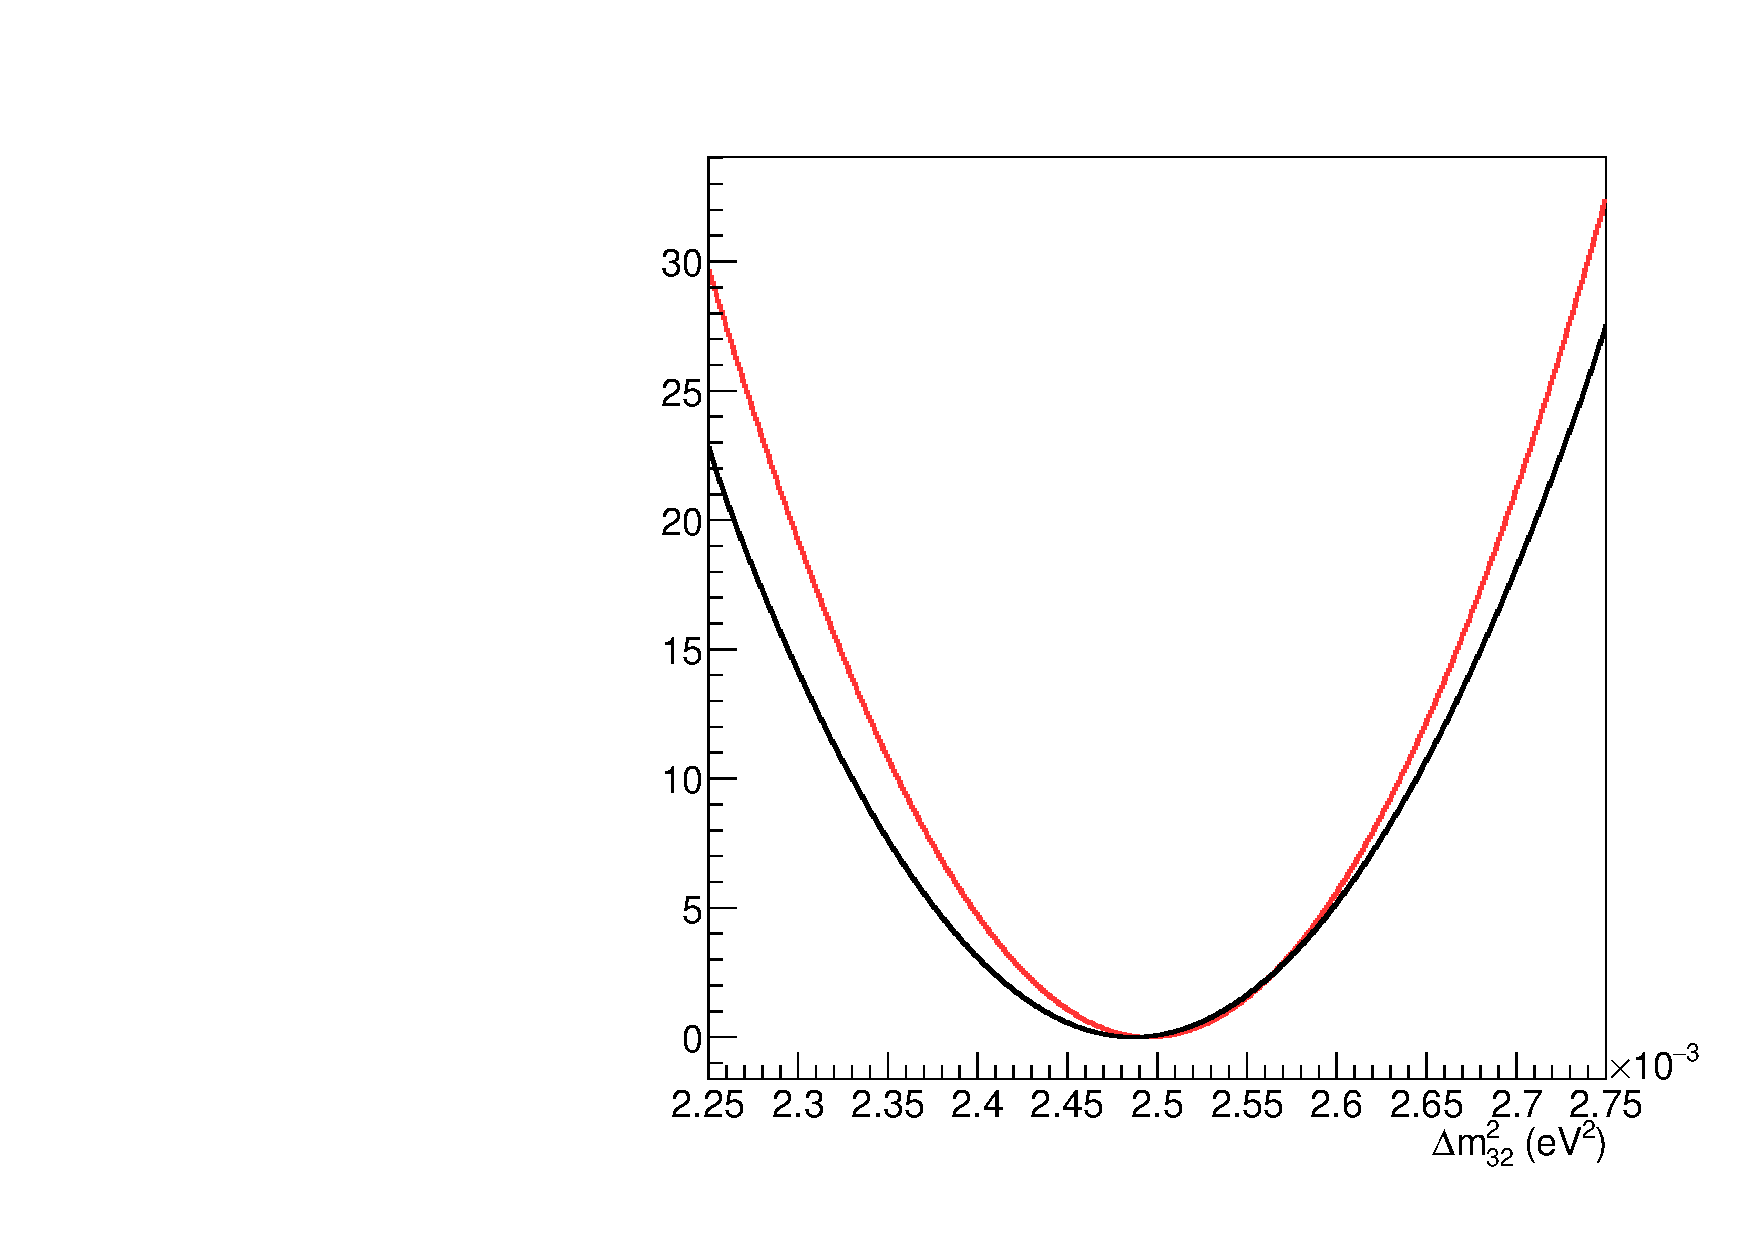
\includegraphics[width=\linewidth]{figs/Section2/section2.6_Rongping_Junjie/globes_t2k_chi2_dm2_comparison_no.pdf}
        \caption{$\Delta\chi^2$ of $\Delta m_{32}^2$}
    \end{subfigure}
    \begin{subfigure}[t]{0.22\textwidth}
        \centering
        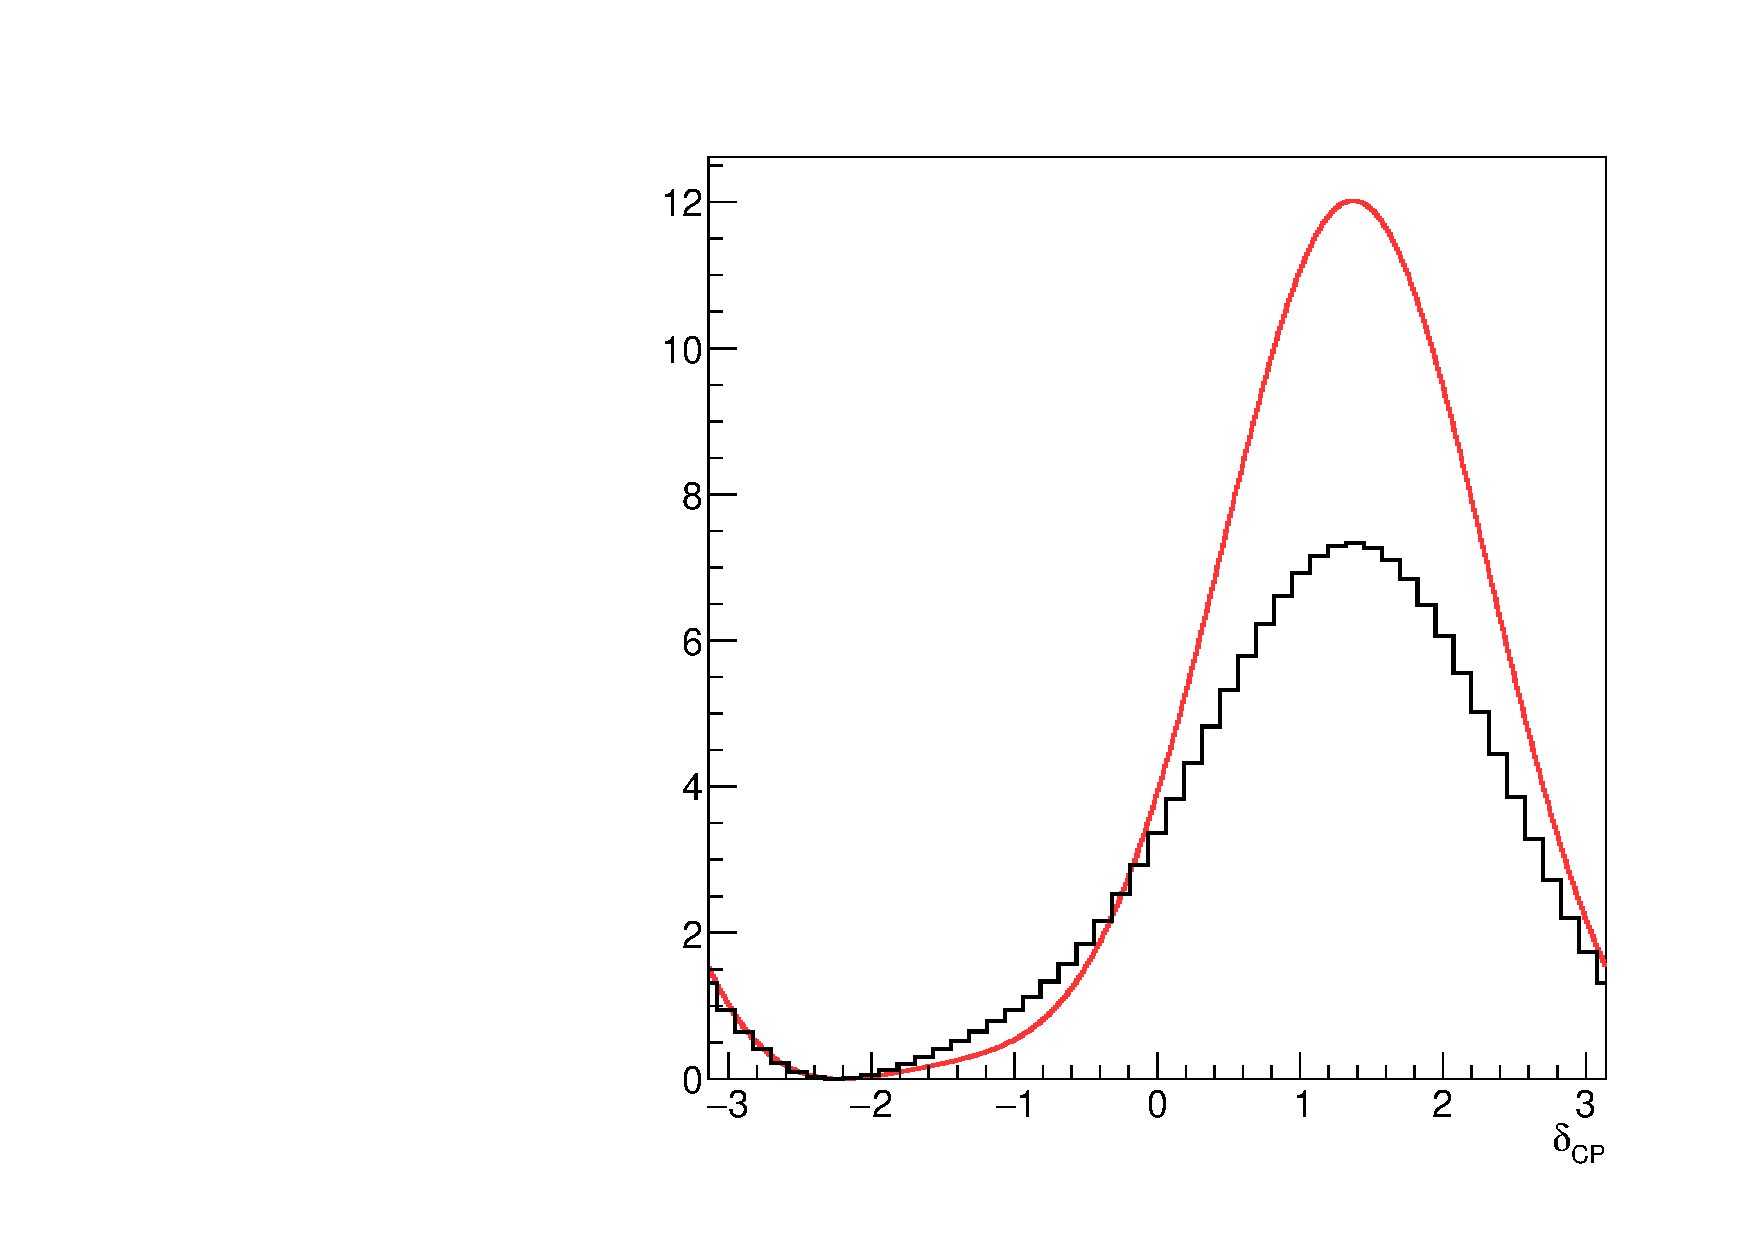
\includegraphics[width=\linewidth]{figs/Section2/section2.6_Rongping_Junjie/globes_t2k_chi2_dcp_comparison_no.pdf}
        \caption{$\Delta\chi^2$ of $\delta_{CP}$}
    \end{subfigure}
    \caption{Comparison of 1D $\Delta\chi^2$ map between GLoBES-T2K (red lines) and T2K published data (black lines) (ref) for oscillation parameters of interest, assuming normal ordering.}
    \label{t2kjuno_junjie:chi2_comparison}
\end{figure}

%LBL fitter+juno external constraints 
%result：juno结果对LBL的NMO 灵敏度的影响
%\item Prediction of potential impact on LBL NMO from JUNO results using the approximated models;
\subsection{Prediction of potential impact}
%%%%%%%%%%%%%%%
%  ONLY FOCUS ON NMO SENSITIVITY
% 1. Spectrum-oriented method (Rongping)
%     1.0 Brief description of how to implement JUNO constraint in the approximated T2K model
%     1.1 Impact from different JUNO DAQ time
%     1.2 Impact of different best-fit values
%
% 2. GLoBES method (Junjie)
%     2.1 Same as 1.1.0
%     2.2 Impact of JUNO's sensitivity and best-fit values on the 'joint' T2K+JUNO NMO sensitivity
%%%%%%%%%%%%%%%
\subsubsection{Spectrum-oriented method}
The spectrum-oriented method can be used to predict the impact of JUNO results as an external constraint on the mass ordering sensitivity of LBL experiments. The method was applied to study different scenarios for both T2K Asimov data and real data. For JUNO results presented in this method, an external constraint on $\theta_{13}$ is applied. For the Asimov T2K case, \autoref{fig:asimov_t2k_zrp} shows a big boost ($\Delta\chi^2=5$) on NMO sensitivity that T2K could get using JUNO (100 days of data taking) as an external constraint. For simplicity, the true values of oscillation parameters are set to PDG2024~\cite{ParticleDataGroup:2024cfk} for both T2K and JUNO. Furthermore, the impact of JUNO DAQ time on the boost is investigated and presented in \autoref{fig:NMO_of_T2k_zrp}. A rapid gain of the boost is observed within the first 100 days of JUNO data taking. But one should note that all the data is Asimov for both T2K and JUNO here, and a strict assumption is put ahead that T2K and JUNO have the same best-fit values on their own. For a more realistic case, \autoref{fig:data_t2k_zrp} displays the potential boosts on T2K-only NMO sensitivity assuming both normal mass ordering (left) and inverted mass ordering (right) using the spectrum-oriented method on real T2K data (ref). Similar to the Asimov case in \autoref{fig:asimov_t2k_zrp}, PDG2024~\cite{ParticleDataGroup:2024cfk} was chosen to be the best-fit values in JUNO 100 days measurements. The boosts in this case become more complicated as it can be either lower (see \autoref{fig:data_t2k_zrp_no}) or higher (see \autoref{fig:data_t2k_zrp_io}) than the T2K-only case. Note that in this case, the best-fit values do not align between T2K-only and JUNO-only. 

\begin{figure}[H]
    \centering
    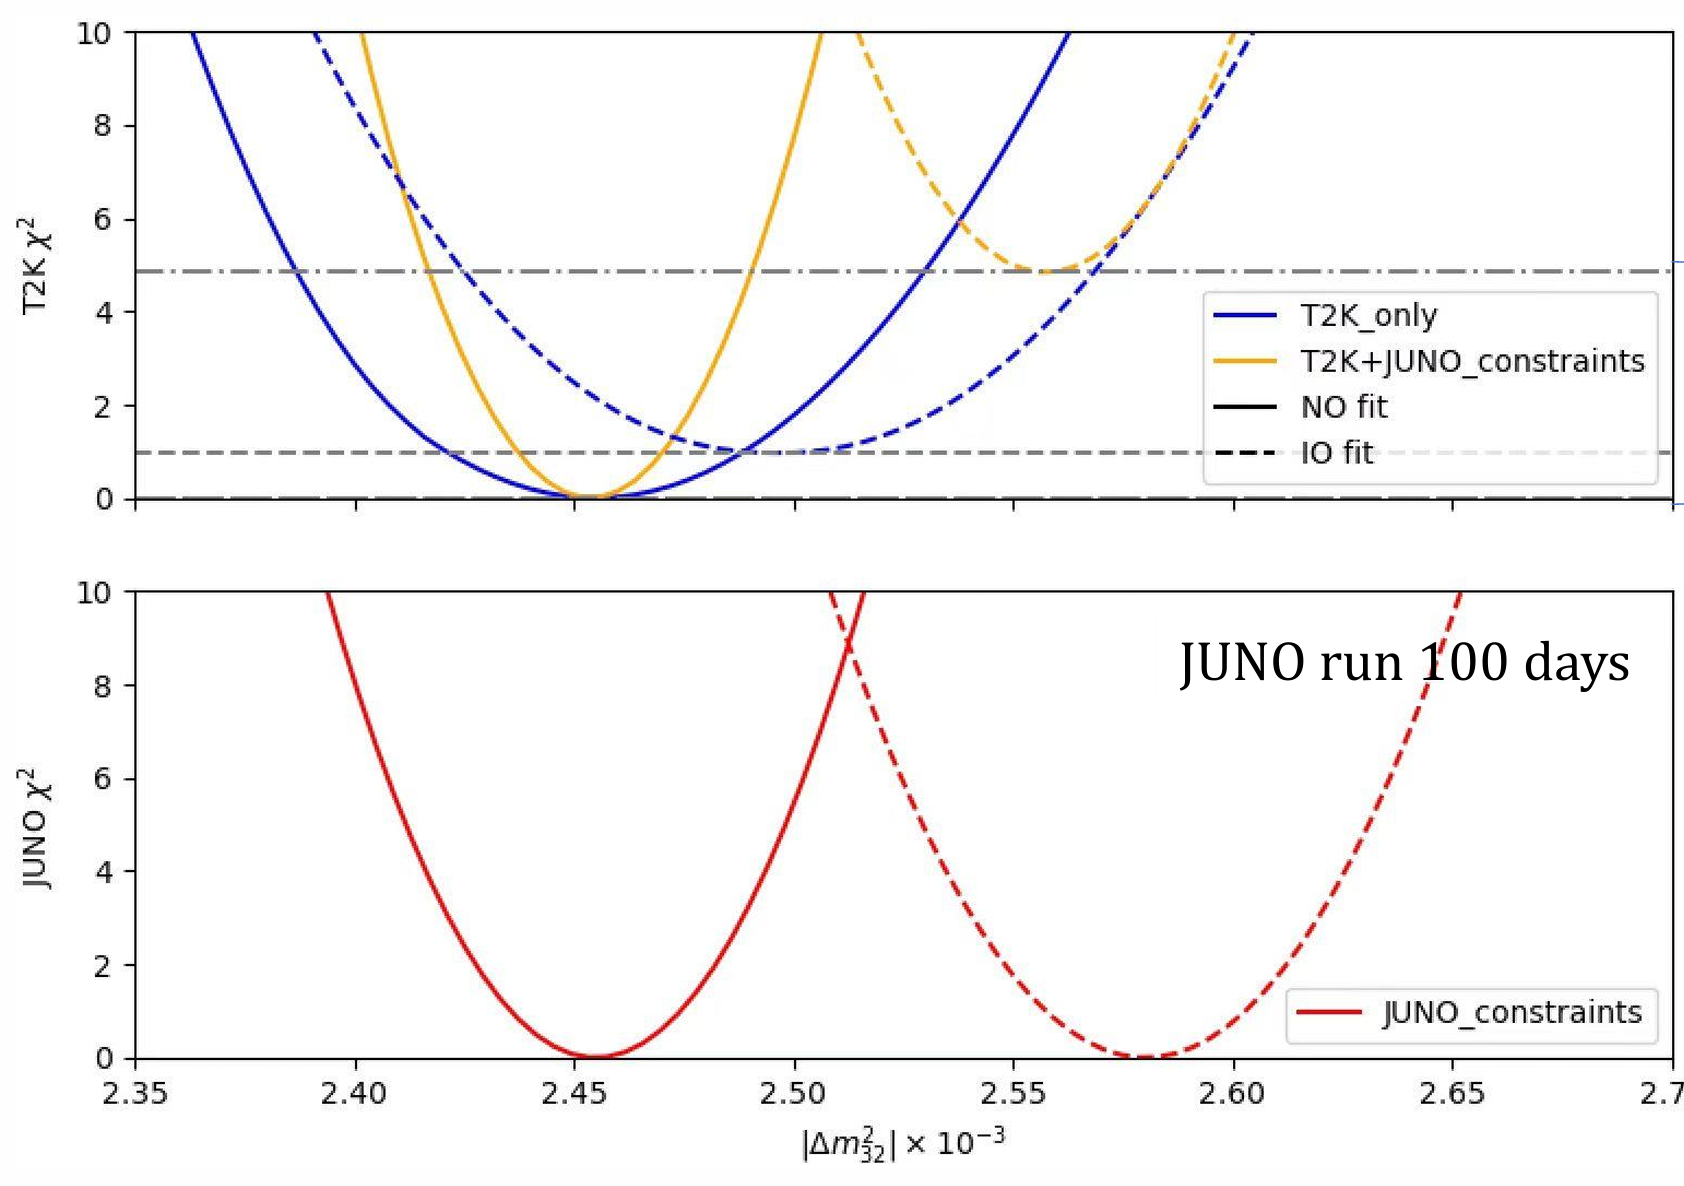
\includegraphics[width=0.45\linewidth]{figs//Section2//section2.6_Rongping_Junjie/asimov_chi2.png}
    \caption{Lower panel: $\chi^2$ of atmospheric mass splitting for JUNO 100 days of data taking, assuming normal mass ordering and the true value is set to PDG2024~\cite{ParticleDataGroup:2024cfk}. Upper panel: boost on Asimov T2K NMO sensitivity from JUNO constraint (yellow contours) compared to Asimov T2K-only case (blue contours), assuming normal mass ordering and the true value is set to PDG2024~\cite{ParticleDataGroup:2024cfk}. Note that the upper panel atmospheric mass splitting scale is different from the lower panel which will be improved soon.}
    \label{fig:asimov_t2k_zrp}
\end{figure}

\begin{figure}[H]
    \centering
    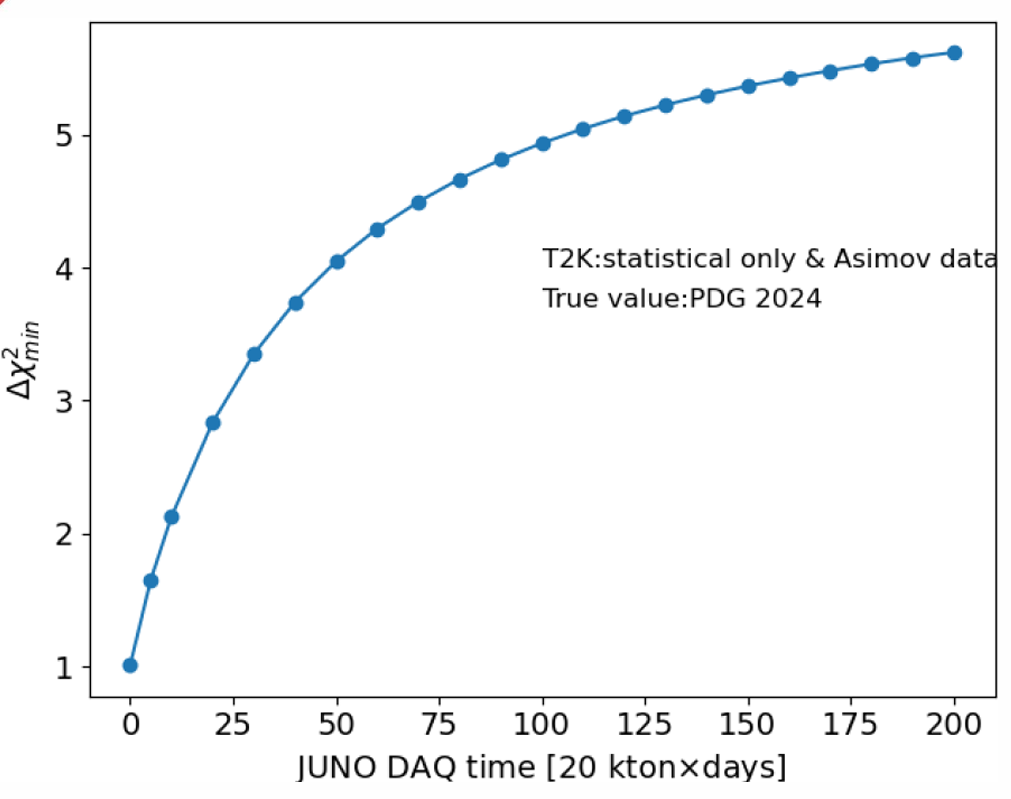
\includegraphics[width=0.45\linewidth]{figs//Section2//section2.6_Rongping_Junjie/t2k_asimov_nmo_sen_zrp.png}
    \caption{NMO sensitivity of Asimov T2K analysis with JUNO as an external constraint for different JUNO DAQ times. The Asimov T2K analysis is produced using the spectrum-oriented method. Normal mass ordering is assumed and true values are set to be PDG2024~\cite{ParticleDataGroup:2024cfk} for both T2K and JUNO.}
    \label{fig:NMO_of_T2k_zrp}
\end{figure}

\begin{figure}[H]
    \centering
    \begin{subfigure}[t]{0.45\textwidth}
        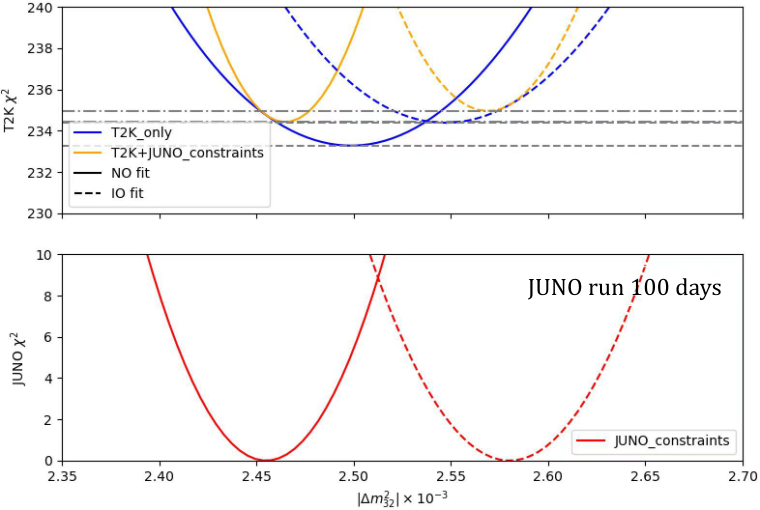
\includegraphics[width=\linewidth]{figs/Section2/section2.6_Rongping_Junjie/t2krealdt_junocon_diffbf_no.png}
    \caption{Normal mass ordering assumption for JUNO}
    \label{fig:data_t2k_zrp_no}
    \end{subfigure}
    \begin{subfigure}[t]{0.45\textwidth}
        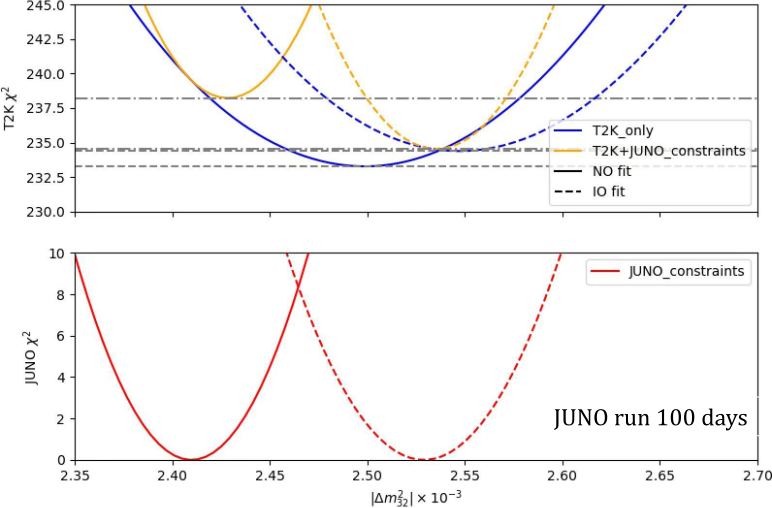
\includegraphics[width=\linewidth]{figs/Section2/section2.6_Rongping_Junjie/t2krealdt_junocon_diffbf_io.png}
    \caption{Inverted mass ordering assumption for JUNO}
    \label{fig:data_t2k_zrp_io}
    \end{subfigure}
    \caption{Lower panel: $\chi^2$ of atmospheric mass splitting for JUNO 100 days of data taking, assuming normal (left) and inverted mass ordering (right) and corresponding true values as PDG2024~\cite{ParticleDataGroup:2024cfk}. Upper panel: boost on T2K NMO sensitivity from JUNO constraint (yellow contours) compared to T2K-only case (blue contours) (ref), assuming normal (left) and inverted mass ordering (right). Note that the upper panel atmospheric mass splitting scale is different from the lower panel which will be improved soon.}
    \label{fig:data_t2k_zrp}
\end{figure}

\subsubsection{GLoBES-based method}
Using the established GLoBES-based T2K model, we tried to double check the conclusion derived in Stephen's study~\cite{Parke:2024xre}. Note that, different from the spectrum-oriented method, all the T2K data used in this method is from T2K OA2020 (ref) instead of T2K OA2024 (ref). As a reminder, the $\Delta\chi_{min}^2$ is defined as,
\begin{equation}
\Delta \chi^2\left(\Delta m_{31}^2 \mid_\mathrm{JUNO}^\mathrm{NO}, \sigma_{\mathrm{JUNO}}\right)_{\min }=\left.\chi_{\mathrm{IO}}^2\right|_{\min }-\left.\chi_{\mathrm{NO}}^2\right|_{\min}
\end{equation}
where $\chi_{\mathrm{NO}}^2$ and $\chi_{\mathrm{IO}}^2$ are defined as,
\begin{equation}
\begin{aligned}
\chi_{\mathrm{NO}}^2\left(\Delta m_{31}^2, \sigma_{\mathrm{JUNO}}\right) & =\chi_{\mathrm{NO}}^2\left(\Delta m_{31}^2, \sigma_{\mathrm{JUNO}}\right)_{\mathrm{JUNO}}+\chi_{\mathrm{NO}}^2\left(\Delta m_{31}^2\right)_{\mathrm{T2K}} \\
\chi_{\mathrm{IO}}^2\left(\left|\Delta m_{32}^2\right|, \sigma_{\mathrm{JUNO}}\right) & =\chi_{\mathrm{IO}}^2\left(\left|\Delta m_{32}^2\right|, \sigma_{\mathrm{JUNO}}\right)_{\mathrm{JUNO}}+\chi_{\mathrm{IO}}^2\left(\left|\Delta m_{32}^2\right|\right)_{\mathrm{T2K}}
\end{aligned}
\end{equation}
Different from the simplified $\chi^2$ approximation for LBL (T2K in our case) in Stephen's study~\cite{Parke:2024xre}, we used the full $\chi^2$ based on the GLoBES approximated T2K model in the above formulas, with the same approximation of JUNO's constraint as Stephen. Marginalization was performed over all systematics for each fit. Four different precisions of JUNO's measurement on the atmospheric mass splitting were selected (i.e. 0.2\%, 0.8\%, 1.3\%, and 3\%) while scanning through the best-fit value of $\Delta m_{31}^2$ in NO fit. The combined $\Delta\chi^2_\mathrm{min}$ is thus obtained as \autoref{t2kjuno_junjie:sens_boost} shows. The value of $\Delta m_{31}^2$ where four color lines intersect is when JUNO's atmospheric mass splitting best-fit value aligns with that of T2K. From \autoref{t2kjuno_junjie:sens_boost}, with improving precision on JUNO's atmospheric mass splitting measurement, the boost on T2K NMO sensitivity becomes greater given the same best-fit value. However, comparing with Stephen's study~\cite{Parke:2024xre}, the boost is not as remarkable as it was predicted in the paper. This can be explained as Stephen used a simplified and combined $\chi^2$ from T2K and NOvA together, which has a better constraint power on the atmospheric mass splitting than T2K alone.
\begin{figure}[H]
    \centering
    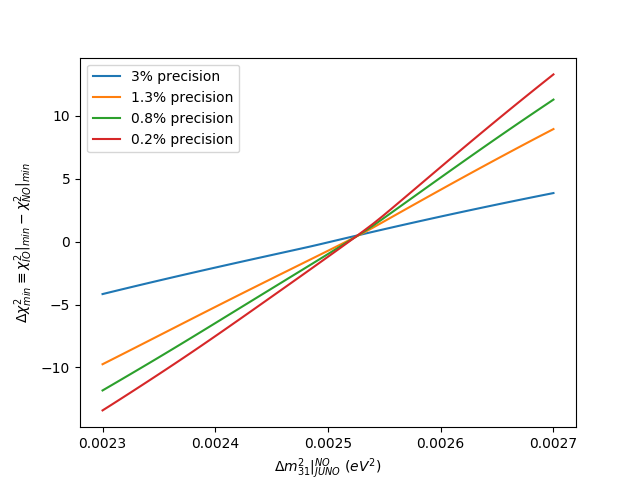
\includegraphics[width=0.5\linewidth]{figs/Section2/section2.6_Rongping_Junjie/globes_t2k_joint_juno_nmo_sens.png}
    \caption{Boosts on T2K NMO sensitivity assuming different precisions from JUNO.}
    \label{t2kjuno_junjie:sens_boost}
\end{figure}

\subsubsection{Discussion}
From the above description of the results from the two methods, we can have a preliminary conclusion that the extra boost gained from JUNO result as an external constraint on T2K-only analysis depends on how different the best-fit values from T2K and JUNO real data and the true value are, as well as JUNO's measurement precision. Due to time constraint, the above two methods have not been applied to the same investigation and thus it is difficult to draw a consistent conclusion based on the presented results.




\section{Summary}
This report presented some of the challenges involved in making a low-statistics ($\lesssim 1$ year) measurement of $\Delta m^2_{31}$ in JUNO. Statistical fluctuations can produce $\Delta\chi^2$ profiles that differ drastically from those obtained using Asimov data sets. Such fluctuations may lead to bad minima, meaning absolute minima that do not correspond to the true value used to generate the data set, as well as to multiple disjoint confidence intervals rather than the single, contiguous one normally expected for a measurement of this kind.

Moreover, the coverage obtained using the standard procedure based on Wilks' theorem, where confidence intervals are defined as regions within a constant value of $\Delta \chi^2$ (such as $\Delta \chi^2=1$ for the $1\sigma$ contour), was shown to be inadequate. This necessitates the implementation of an alternative approach, such as Feldman–Cousins, in which confidence intervals are derived from large ensembles of pseudo-experiments that include both statistical and systematic fluctuations. This, in turn, significantly increases the complexity and computational demands of the analysis.

It was demonstrated that these challenges affect almost exclusively the measurement of $\Delta m^2_{31}$ and not the solar parameters $\Delta m^2_{21}$ and $\sin^2\theta_{12}$, although care must still be taken to avoid biases associated with low-statistics bins. While not insurmountable, these challenges must be properly addressed to ensure an accurate determination of $\Delta m^2_{31}$. All this implies that the published $\Delta m^2_{31}$ sensitivities of Ref.~\cite{JUNO:2022osc}, which are based on Asimov data sets, have some limitations in that they do not capture all relevant statistical effects. In particular, low-statistics measurements of $\Delta m^2_{31}$ will not produce a single confidence interval matching the precision of the Asimov sensitivities with high probability. However, they remain largely accurate for larger exposures, corresponding to approximately one year of data or more.

This report also explored a potential mitigation strategy to avoid the occurrence of multiple disjoint intervals, which involves applying an external constraint on $\Delta m^2_{31}$. In this work, we examined the option of using a constraint from the Daya Bay experiment, although others could be used in principle. In this case, the external information helps the JUNO fit focus on the correct minimum, thereby drastically reducing the probability of obtaining multiple intervals. The drawback is that it makes the JUNO result dependent on external constraints.

The use of Daya Bay data to constrain the reactor antineutrino spectral shape was also explored, motivated by the fact that TAO data will likely not be available for the first low-statistics measurement of the oscillation parameters. This study presented a viable approach for incorporating the Daya Bay information through a joint fit with JUNO, starting from a common reactor antineutrino model that is allowed to vary. It was found that a precision comparable to that achievable with TAO can be obtained, with only a modest degradation in sensitivity observed for $\Delta m^2_{31}$. 

Finally, the potential impact of a low-statistics JUNO measurement of $\Delta m^2_{31}$ on the mass ordering determination of ongoing long-baseline accelerator experiments was also investigated. As expected, the extent of this impact depends primarily on the best-fit value and the precision achieved by JUNO for $\Delta m^2_{31}$. In some scenarios, the improvement can be substantial, potentially enabling a $3\sigma$ determination of the mass ordering.

\printbibliography[heading=bibintoc]

\newpage

\begin{appendices}
\section{Fitting Techniques}
\label{app:fit}


To perform a fit, a classical approach is to maximize a likelihood derived from the probability to observe the distribution to fit in the available sample, given the PDF from which it is assumed to be drawn.

In the case of a binned distribution, assuming that the dataset is sufficiently large to ensure an asymptotic behavior and assuming the effect of systematic uncertainties is also gaussian, the above-mentioned probability is approximated by a multidimensional gaussian distribution, as is the likelihood:
\begin{equation}
\label{eq:likelihoodMultiGauss}
	{\cal L} \equiv \mathcal{P}= \frac{1}{\sqrt{(2\pi)^N|V|}}e^{-\frac{1}{2}\left(  \boldsymbol{x-\mu(\theta,\eta)}  \right)^TV^{-1}\left(  \boldsymbol{x-\mu(\theta,\eta)}  \right)  }
\end{equation}
where $N$ is the number of bins, \textit{\textbf{x}} the vector containing the number of entries in each bin in the data,   $\mathbf{\mu}$  the vector containing the predictions based on the modeled PDF of the energy distribution, $\mathbf{\theta}$ the oscillation parameters, $\mathbf{\eta}$ the vector containing the nuisance parameters and $V$ the covariance matrix, made of a component accounting for statistical fluctuations and another one accounting for systematic uncertainties, $V = V_{stat}+V_{syst}$. 

Replacing the maximization of ${\cal L}$ by the minimization of $-2ln\mathcal{L}$ implies to minimize:
\begin{equation}
	\chi^2\equiv-2ln\mathcal{L}=\left(\boldsymbol{x-\mu(\theta,\eta)}\right)^T\cdot \boldsymbol V^{-1}\cdot \left(\boldsymbol{x-\mu(\theta,\eta)}\right)+ln|V|,
	\label{eq:chi_sq}
\end{equation}

The frameworks used to produce the results presented in this note minimize several versions of this test statistics. They differ in the way they treat $V_{stat}$ and in the way they treat the systematic uncertainties. 


The $V_{stat}$ matrix is a diagonal matrix which elements are an evaluation of the uncertainty on the number of entries in each bin. It's equivalent to evaluate the expectation value of this number according to the Poisson statistics. In the Neyman approach, the observations \textit{\textbf{x}} are used, while the Pearson approach uses the predictions $\mathbf{\mu}(\theta,\eta)$. Both approaches neglect the dependence of $ln|V|$ on $\mathbf{\theta}$ and $\mathbf{\eta}$ , removing it from their formulation. They are both known to potentially bias the evaluation of the $\mathbf{\theta}$ parameters resulting from the fit. In~\cite{Ji_2020}, a combined Neyman Pearson test statistics was introduced, where 
\begin{equation}
	V_{stat} = \frac{1}{3}V_{stat}^{Neyman}+\frac{2}{3}V_{stat}^{Pearson}
\end{equation}
It allows, to an extent which depends on the specifics of the fit under consideration, to reduce the bias. The respective biases affecting the Pearson and Neyman approaches compensating each other. We will call this test statistic $\chi^2_{CNP}$. Some studies observed that in certain conditions a bias (particularly on $sin^2\theta_{12}$) remains when using $\chi^2_{CNP}$. It can be solved by using the Pearson approach {\it without} neglecting $ln|V|$, i.e. by being consistent with the probability law data are assumed to be drawn from. We call the corresponding test statistics $\chi^2_{Pearson+lnV}$ .


The systematic uncertainties are accounted for either via the $V_{syst}$ part of the covariance matrix or by letting nuisance parameters vary during minimization. This variation is constrained according to prior evaluations of these parameters. Assuming for these evaluations a gaussian behavior (and therefore that gaussians multiply the right hand side of 
Eq.~\ref{eq:likelihoodMultiGauss}) pull terms arise in the test statistics: 
\begin{equation}
	\chi^2 =\left(\boldsymbol{x-\mu(\theta,\eta)}\right)^T\cdot \boldsymbol V^{-1}\cdot \left(\boldsymbol{x-\mu(\theta,\eta)}\right) + ln|V| + \sum_{i}\left(\frac{\eta_{i}-\bar{\eta}_i}{\sigma_{i}}\right)^{2},
	\label{eq:chi_sq}
\end{equation}
where $\bar{\eta}_i$'s are the prior preferred values of the nuisance parameters and $\sigma_i$'s
the uncertainties on this prior knowledge and where we assume no correlations among $\eta_i$'s. Although it's possible in principle to treat all systematic effects via nuisance parameters, it's often easier or more practical to still treat some of them via $V_{syst}$.

The studies presented in this note have been carried out using 4 frameworks: ORSA, GNA, IHEP and AveNue. Results from all of them are discussed in Sections~\ref{sec:LowStatMeas} and~\ref{sec:NMOwithLBL}. 
Table~\ref{tab:Framewk_options} specifies the test statistics used by each framework and the methods adopted to incorporate statistical effects.

\begin{table}[h]
\centering
\begin{tabular}{lccc|cc}
\toprule
Framework & $\chi^2_{CNP}$ & $\chi^2_{Pearson}$ & $\chi^2_{Pearson+lnV}$ & $V_{syst}$ & Nuisance \\
\midrule
ORSA      & asimov  & -      & pseudosamples & spectrum b2b  & All others \\
AveNue    & -       & asimov & pseudosamples &    All        &  \\
IHEP      & asimov  & -      & pseudosamples & spectrum b2b   & All others\\
GNA       & asimov  & -      & pseudosamples &  spectrum b2b   & All others \\
\bottomrule
\end{tabular}
\caption{Test statistics used by each framework and the methods adopted to incorporate statistical effects. Here,the terms "Asimov" and "pseudosamples" designate the cases where fits to an Asimov sample or to pseudosamples are performed. The right part of the table explains which systematic effects are treated via the covariance matrix and which are treated via nuisance parameters.}
\label{tab:Framewk_options}
\end{table}

In addition to the Gaussian-based approximations discussed above, the Poisson-based test statistic is also widely used, especially when dealing with small event counts or in cases where the Gaussian approximation may not be valid. This approach starts from the exact Poisson likelihood, which reflects the probability of observing a certain number of counts in each bin given the expected value.
For each bin $i$, the Poisson probability of observing $x_i$ events given the predicted count $\mu_i$ is

$$P(x_i \mid \mu_i) = \frac{\mu_i^{x_i} e^{-\mu_i}}{x_i!}.$$
For a binned dataset with independent Poisson-distributed entries, the log-likelihood can be written as:

\begin{equation}  
\label{eq:poisson_like}  
\ln \mathcal{L}_{Poisson} = \sum_{i} \left( x_i \ln \mu_i(\theta, \eta) - \mu_i(\theta, \eta) - \ln x_i! \right),  
\end{equation}

where $x_i$ is the observed count in bin $i$, and $\mu_i(\theta, \eta)$ is the predicted count depending on oscillation parameters $\theta$ and nuisance parameters $\eta$.

Dropping the constant term $\ln x_i!$, which does not depend on the fit parameters, and defining a test statistic based on the negative log-likelihood gives the so-called Poisson $\chi^2$:

\begin{equation}  
\chi^2_{Poisson} = 2 \sum_{i} \left( \mu_i(\theta, \eta) - x_i + x_i \ln \frac{x_i}{\mu_i(\theta, \eta)} \right),  
\label{eq:chi2_poisson}  
\end{equation}

This test statistic does not rely on the Gaussian approximation and is particularly useful in low-statistics low exposure. When systematic uncertainties are included, they are typically handled through nuisance parameters with pull terms added in the $\chi^2$ function Eq.~\ref{eq:chi2_poisson}:

\begin{equation}  
\chi^2 = \chi^2_{Poisson} + \sum_{i}\left(\frac{\eta_{i}-\bar{\eta}_i}{\sigma_{i}}\right)^2.  
\end{equation}

This approach ensures full consistency with the Poisson probability law from which the observed data are drawn, and avoids the potential biases arising from approximating the statistical uncertainty using Gaussian distributions.

At IHEP, the Poisson-based fitter has been fully developed and validated. It is now ready for application in the first physics publication based on low-exposure data.

\section{Pseudo-Experiment Generation}\label{appendix:pseudoexp}

Most of the analyses presented in this note are based on a large number pseudo experiments, each consisting of fitting a toy energy distribution, randomly drawn from a model of this distribution. The values of the parameters the model depends on, as well as the uncertainties up to which they are expected to be known -- that are necessary to determine the fluctuations between toy distributions -- are close to those assumed in JUNO’s recent NMO sensitivity paper~\cite{JUNO:2024jaw}. There are few updates are worth mentioning: 
\begin{itemize}
    \item The reference values of $\Delta m^2_{21}$, $\sin^2(\theta_{12})$ and $\sin^2(\theta_{13})$ are taken from the 2024 issue of the PDG (instead of 2020) and that for $\Delta m^2_{31}$ is set to Daya Bay 's measurement (save for AveNuE). 
    \item  The antineutrino spectrum bin-to-bin shape uncertainty is assumed to be provided by TAO's spectrum,  scaling its statistical part according to the exposure. In particular, this replaces the combined JUNO+TAO fit presented in~\cite{JUNO:2024jaw}. 
\end{itemize}

In addition to statistical fluctuations, the pseudosamples used in the studies  presented in this document also incorporate 
the fluctuations needed to account  for systematic uncertainties. The Avenue framework proceeds in two steps to produce a pseudosample:
\begin{itemize}
    \item First, it distorts the PDF computed with the nominal values of the parameters involved in this theoretical model of the energy distribution. Each component is adjusted by adding a random shift vector, $\vec{\delta \mu}$, to the prediction vector, $\vec{\mu}(\theta,\eta)$  (see section~\ref{app:fit}). The elements of this vector are drawn from an N-dimensional Gaussian distribution, whose covariance matrix is the systematic component ($V_{syst}$) of the covariance matrix used in the $\chi^2$ minimized by the fit. To simplify this problem into a series of independent one-dimensional Gaussian draws, despite the correlations among the  $\delta\mu_i$’s, a Cholesky decomposition is carried out.
    \item Second, the toy energy distribution with statistical fluctuations is generated: the number of entries in each bin is drawn from a Poisson distribution with an expectation of  $\mu_i+\delta \mu_i$.
\end{itemize}
The studies based on the other frameworks proceed in three steps:
\begin{itemize}
    \item First, random values of the PDF’s parameters treated as nuisance parameters are drawn from the multidimensional Gaussian that encompasses the prior knowledge of them. 
    \item Second, the PDF of the energy distribution is computed using these values.
    \item Finally, a pseudo sample is drawn from this PDF to incorporate statistical fluctuations.
\end{itemize}



\end{appendices}

\end{document}
